\appendix

\section{Additional Results for Different Harmonic Configurations}

This appendix presents comprehensive results for all tested harmonic configurations, demonstrating the non-monotonic relationship between harmonic count and solution accuracy. Each configuration was trained using the identical two-phase optimization strategy described in the main text.

\subsection{Three-Dimensional Solution Visualizations}

\begin{figure}[H]
    \centering
    \begin{subfigure}[b]{0.48\textwidth}
        \centering
        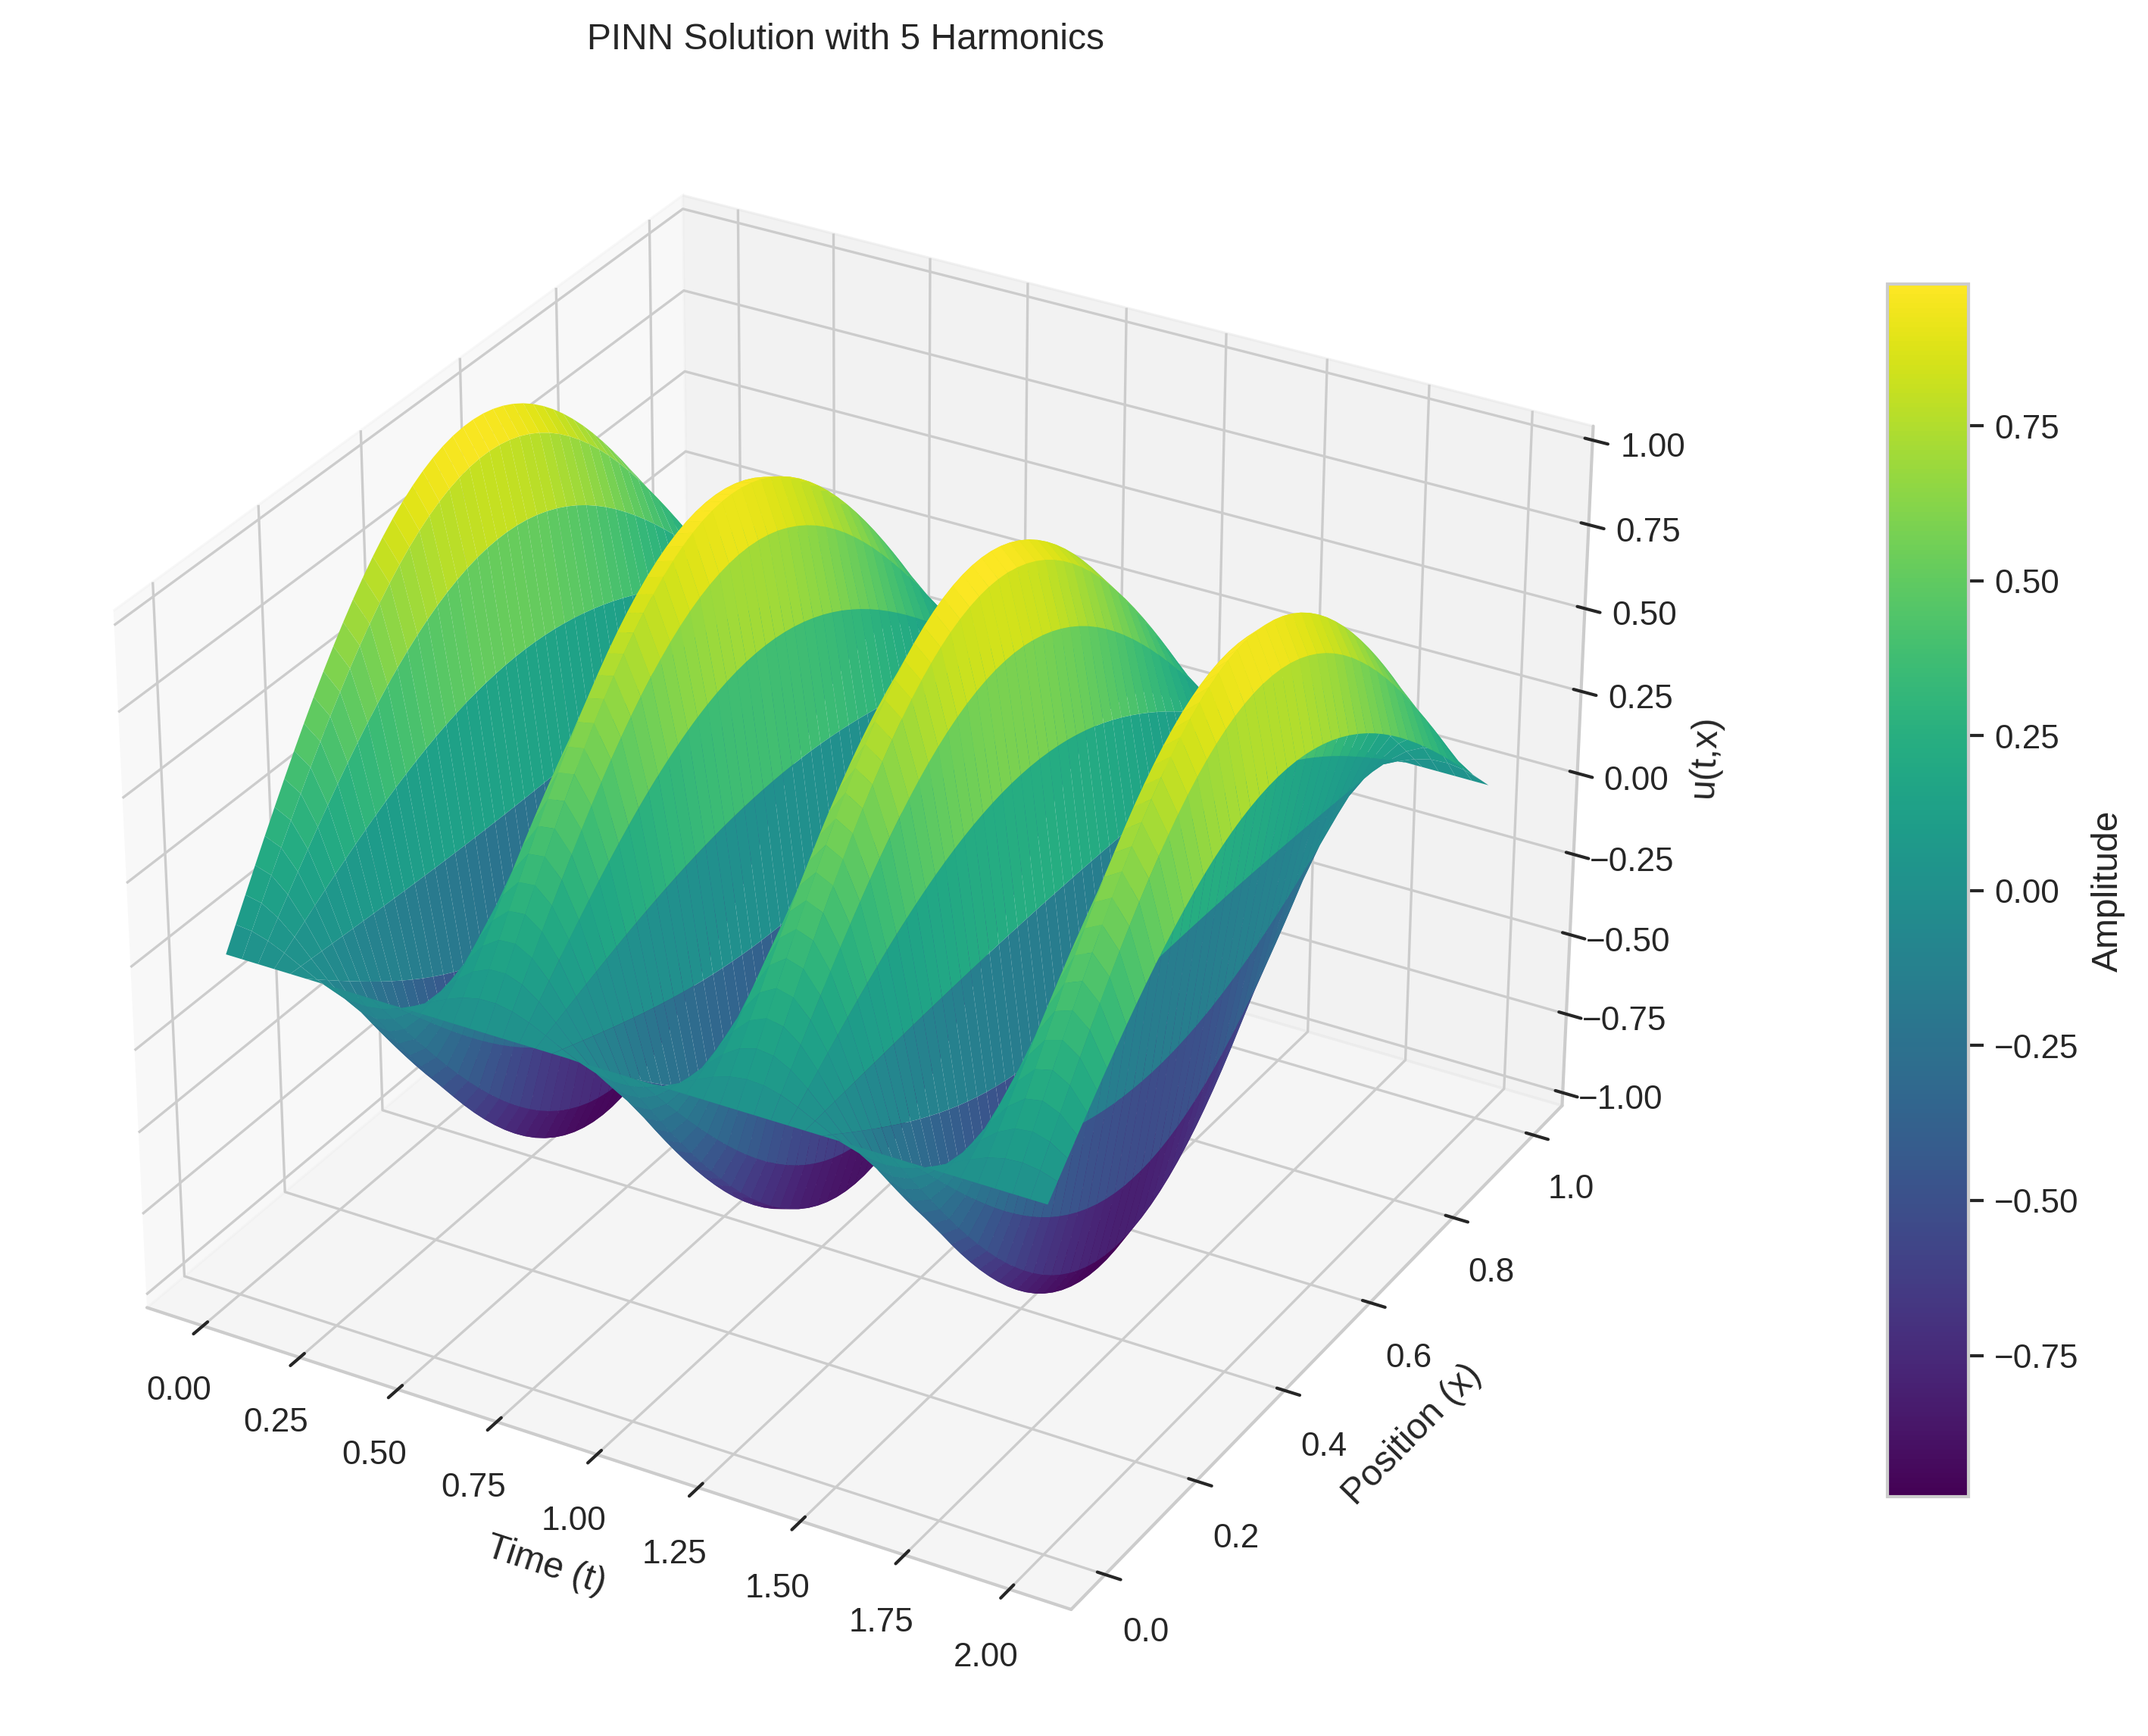
\includegraphics[width=\textwidth]{figures/3d_comparison_pinn_solution_5h.png}
        \caption{5 harmonics}
        \label{fig:3d_5h}
    \end{subfigure}
    \hfill
    \begin{subfigure}[b]{0.48\textwidth}
        \centering
        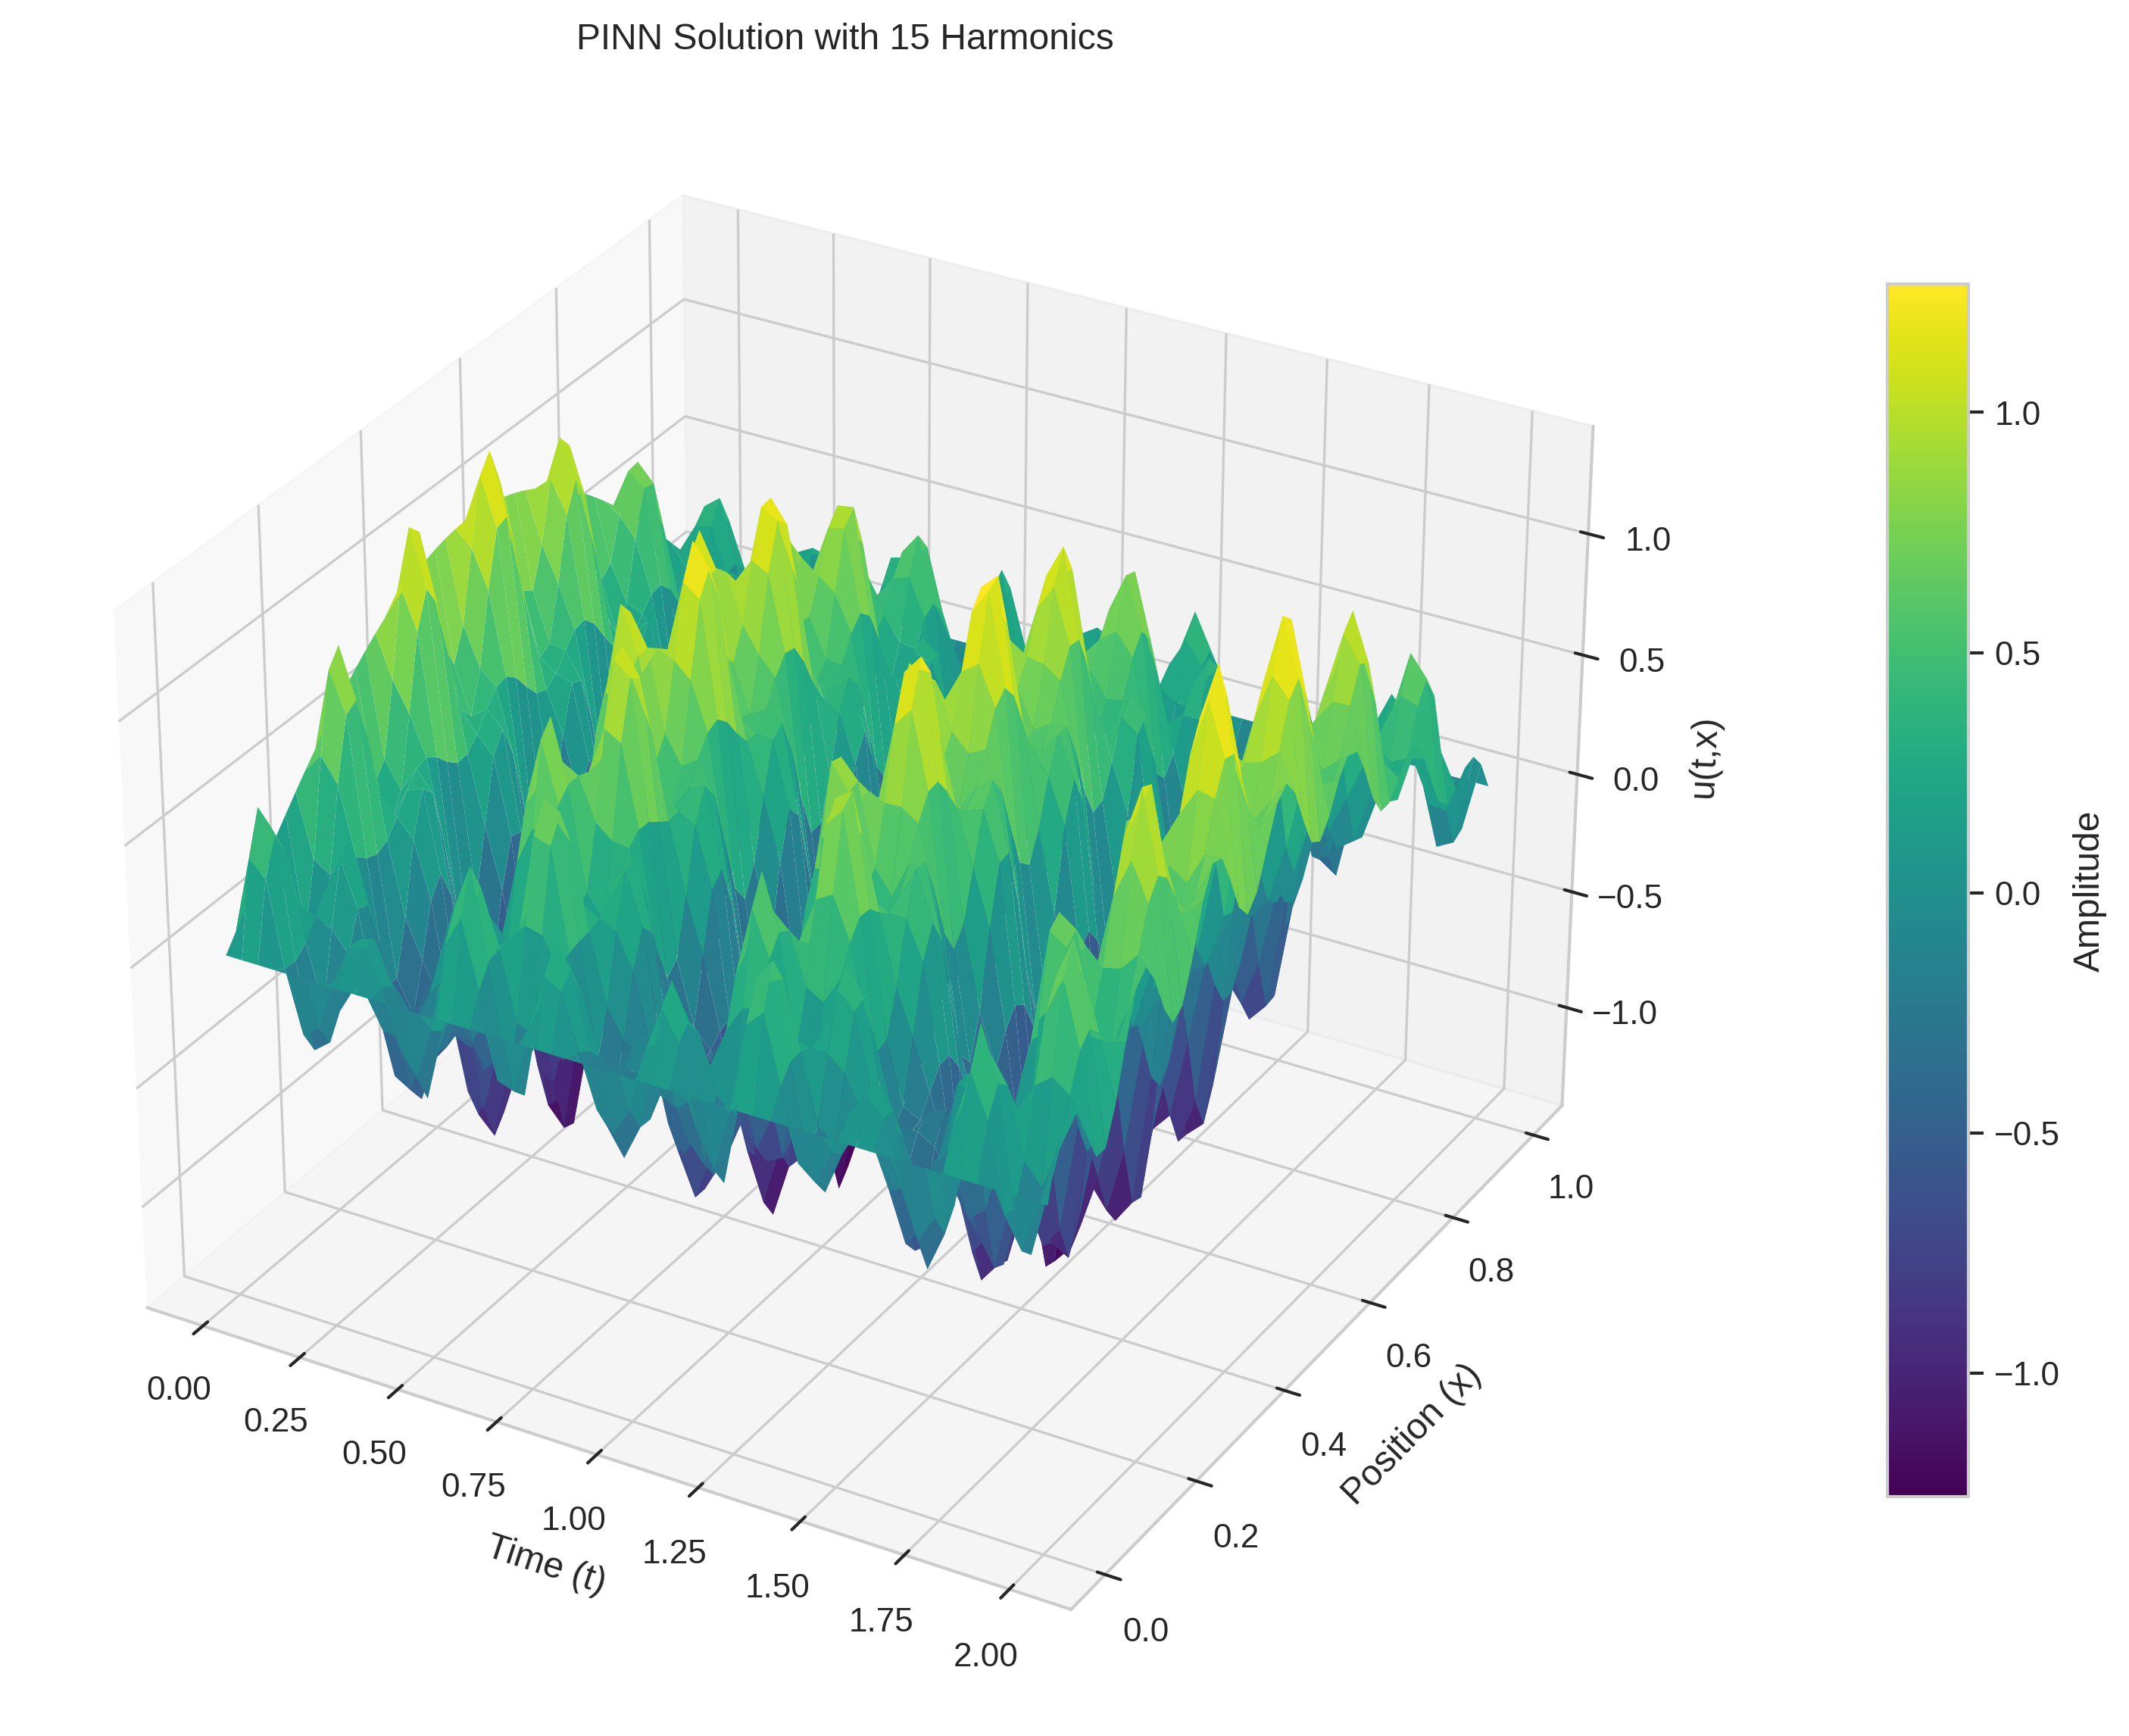
\includegraphics[width=\textwidth]{figures/3d_comparison_pinn_solution_15h.png}
        \caption{15 harmonics}
        \label{fig:3d_15h}
    \end{subfigure}
    \caption{Three-dimensional solution profiles for 5 and 15 harmonics, showing the dramatic degradation in accuracy beyond the optimal configuration.}
    \label{fig:3d_comparison}
\end{figure}

\begin{figure}[H]
    \centering
    \begin{subfigure}[b]{0.48\textwidth}
        \centering
        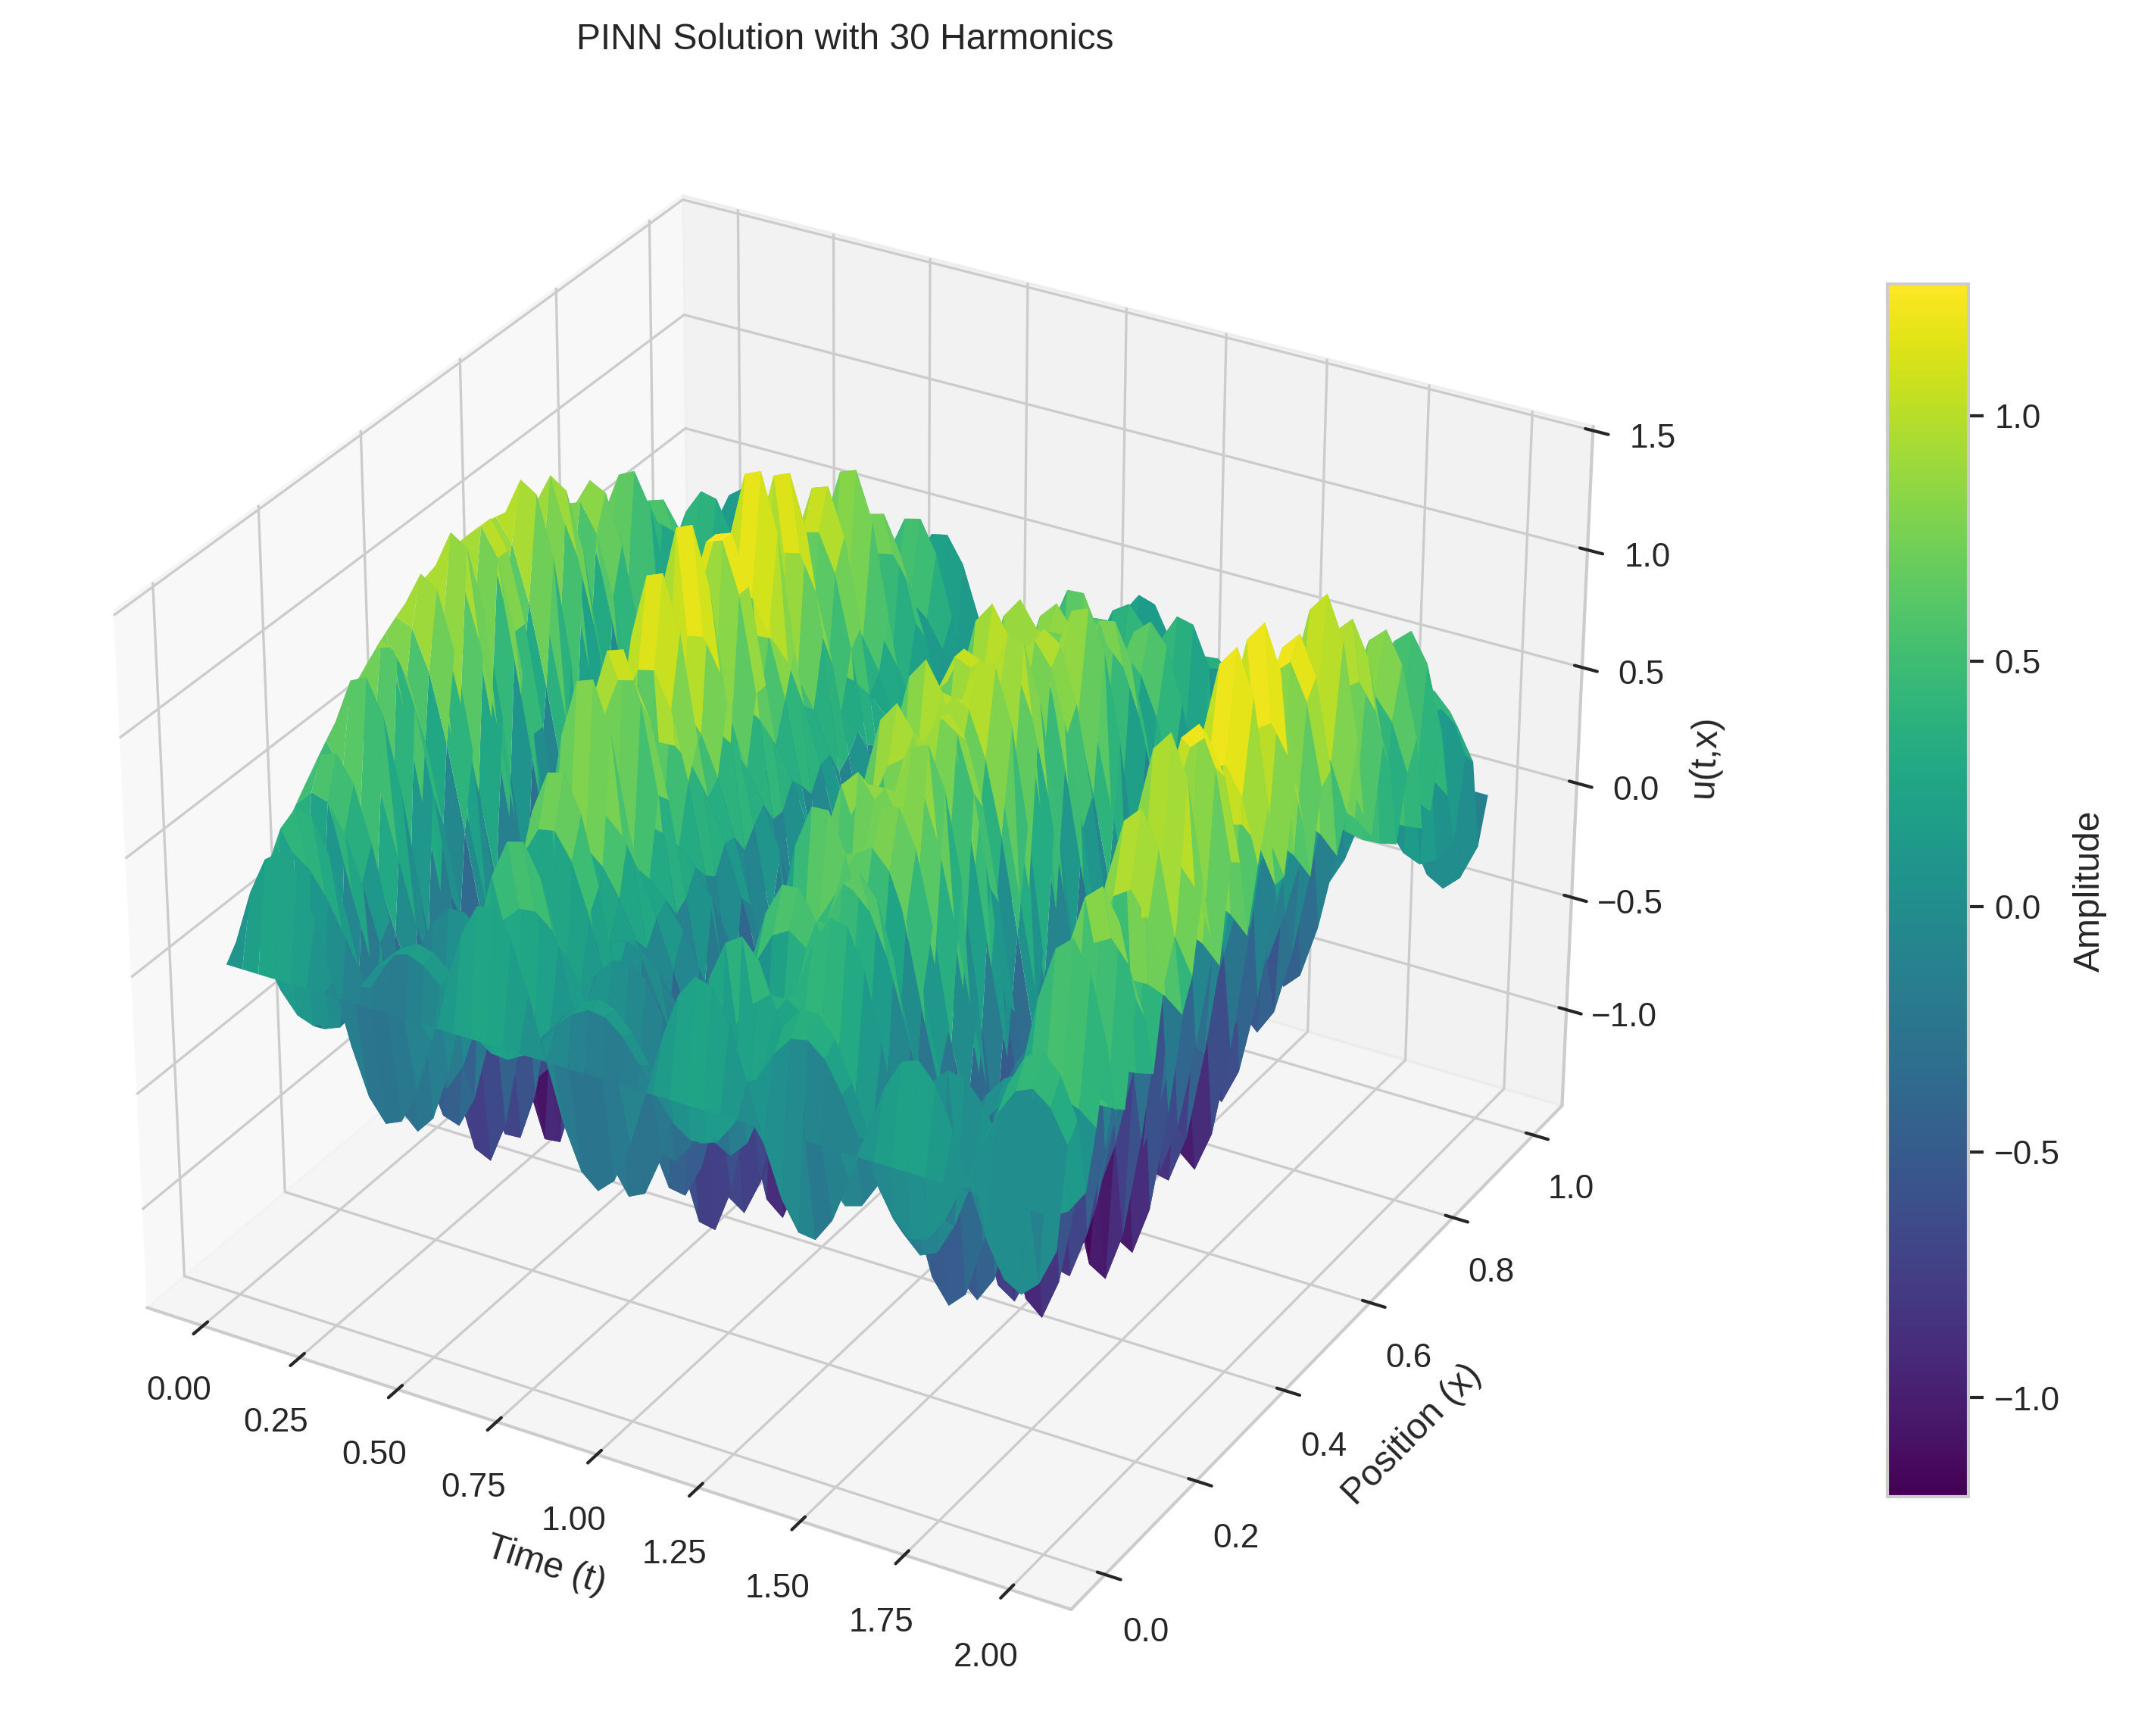
\includegraphics[width=\textwidth]{figures/3d_comparison_pinn_solution_30h.png}
        \caption{30 harmonics}
        \label{fig:3d_30h}
    \end{subfigure}
    \hfill
    \begin{subfigure}[b]{0.48\textwidth}
        \centering
        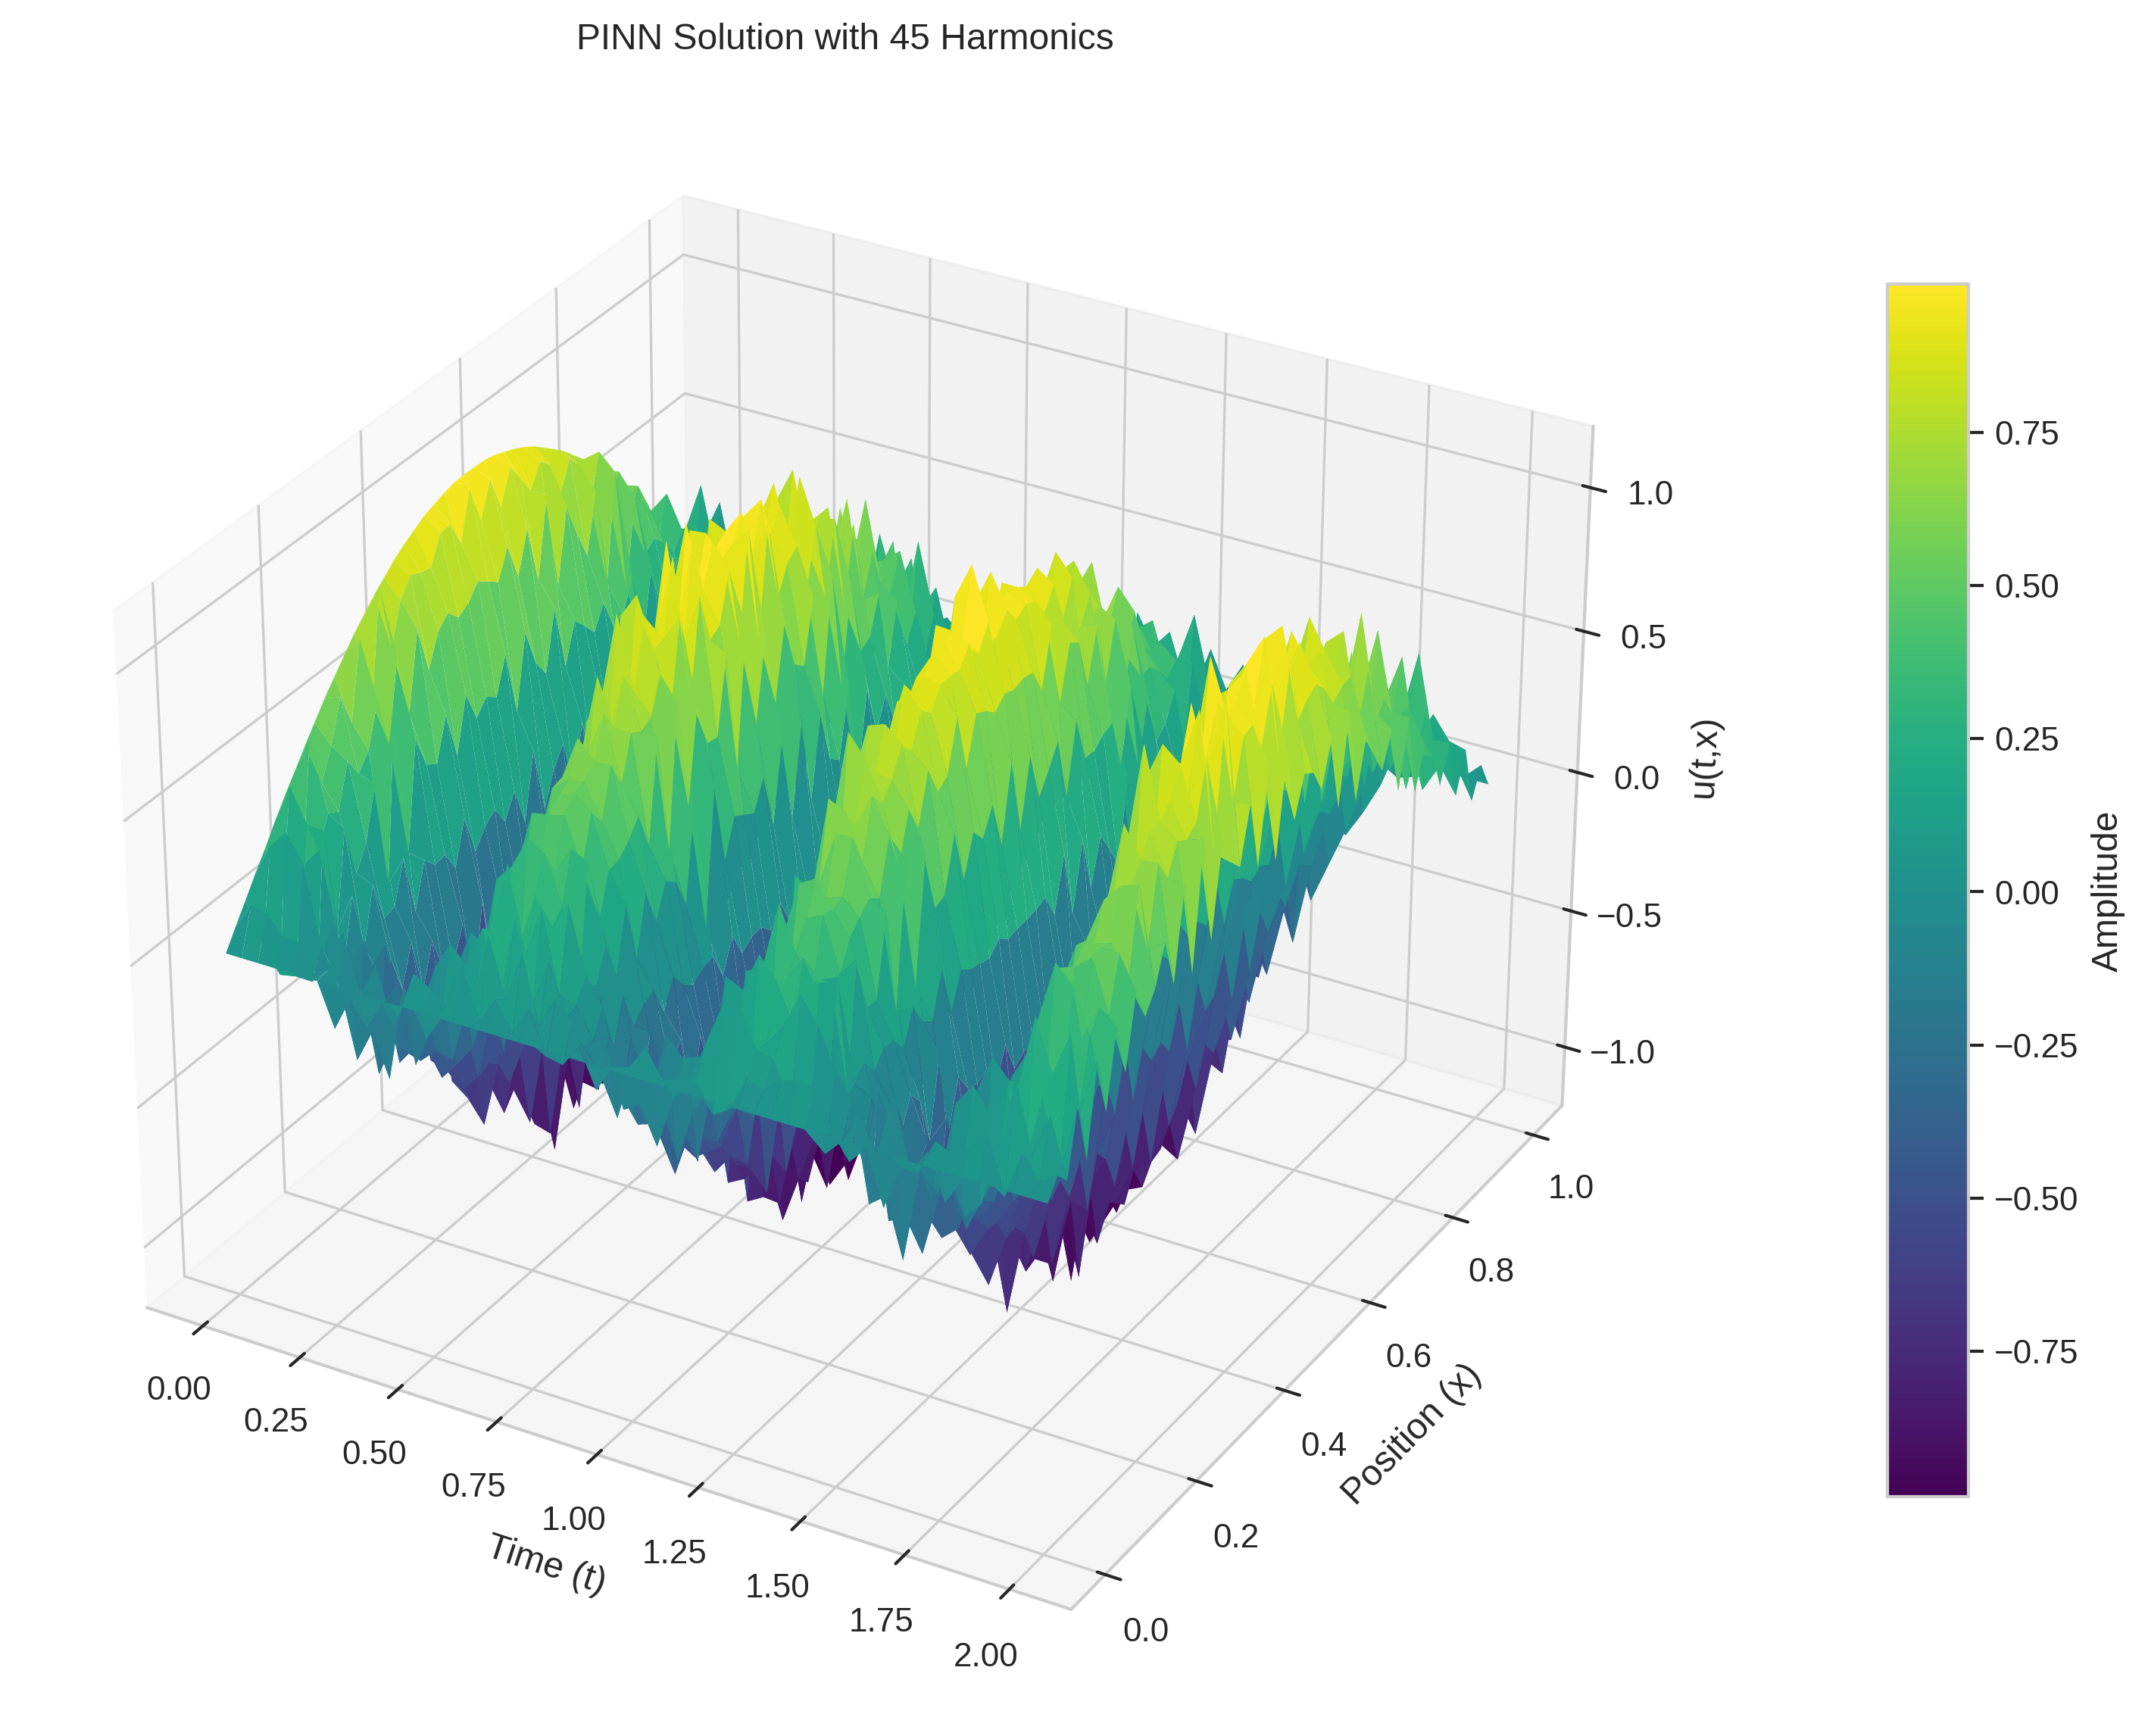
\includegraphics[width=\textwidth]{figures/3d_comparison_pinn_solution_45h.png}
        \caption{45 harmonics}
        \label{fig:3d_45h}
    \end{subfigure}
    \caption{Higher harmonic configurations (30 and 45) demonstrate significant accuracy degradation due to optimization challenges in high-dimensional parameter spaces.}
    \label{fig:3d_high_harmonics}
\end{figure}

\subsection{Error Distribution Analysis}

\begin{figure}[H]
    \centering
    \begin{subfigure}[b]{0.32\textwidth}
        \centering
        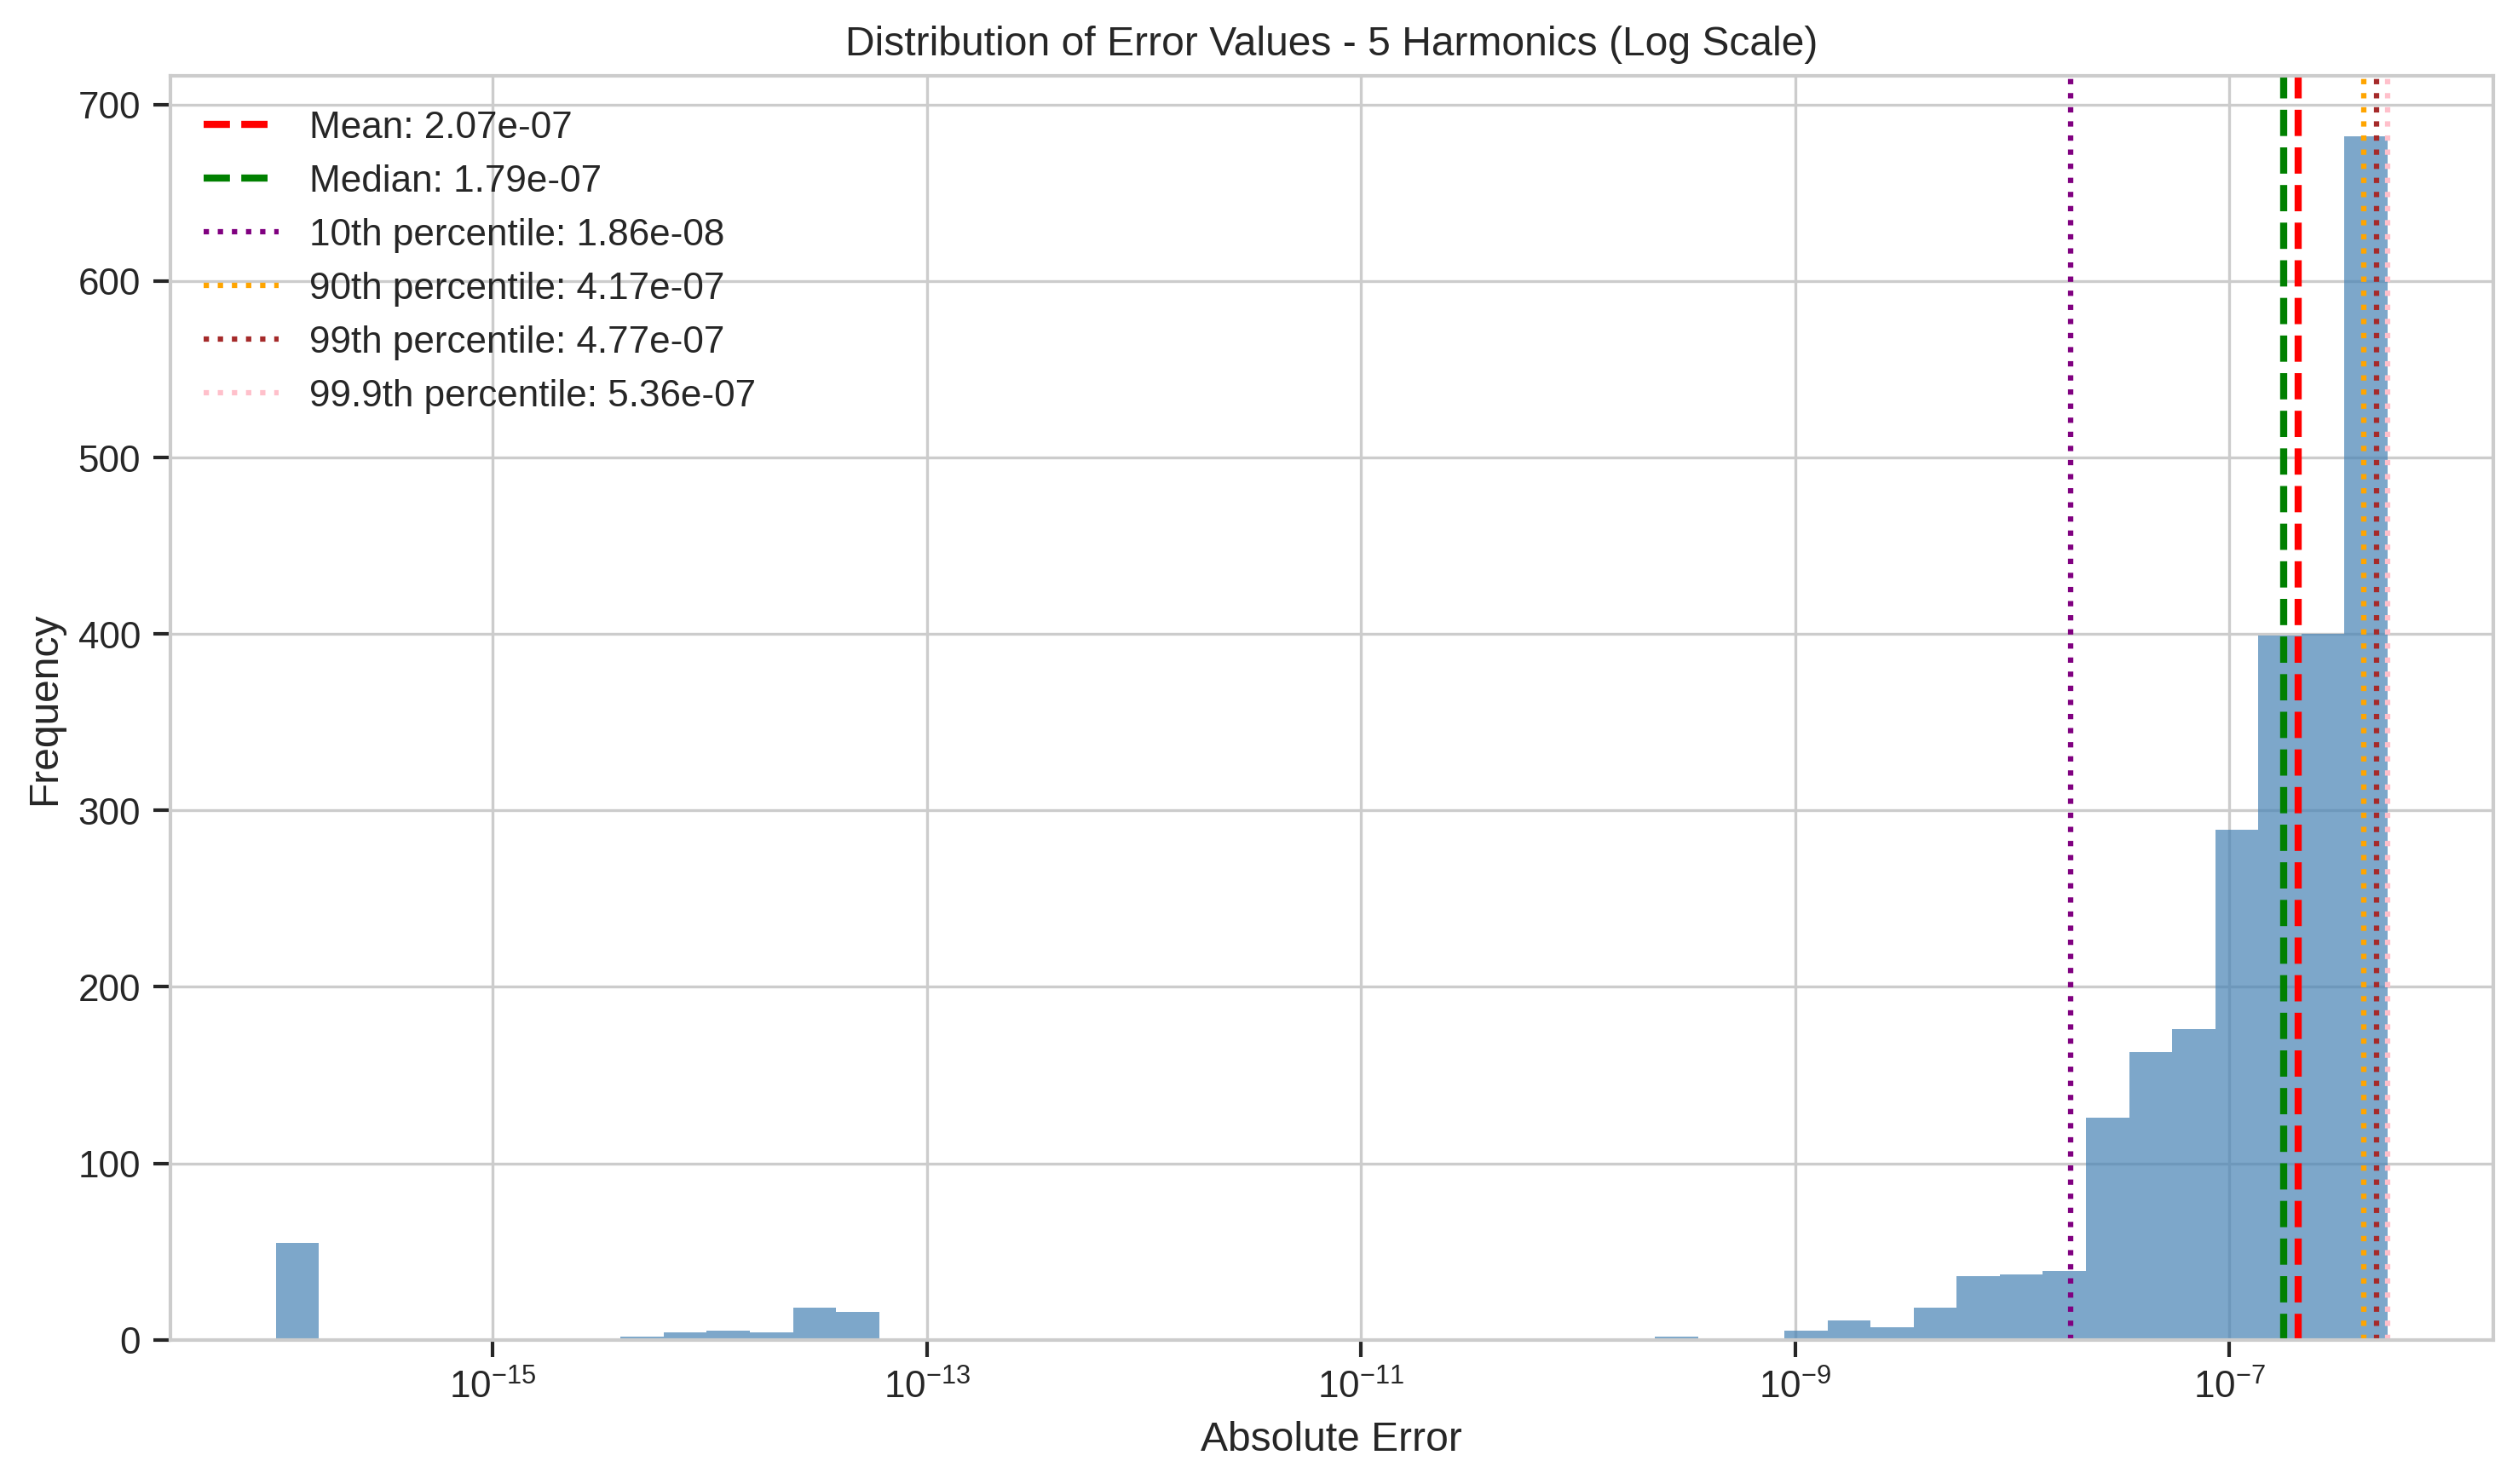
\includegraphics[width=\textwidth]{figures/error_distribution_5h.png}
        \caption{5 harmonics}
    \end{subfigure}
    \hfill
    \begin{subfigure}[b]{0.32\textwidth}
        \centering
        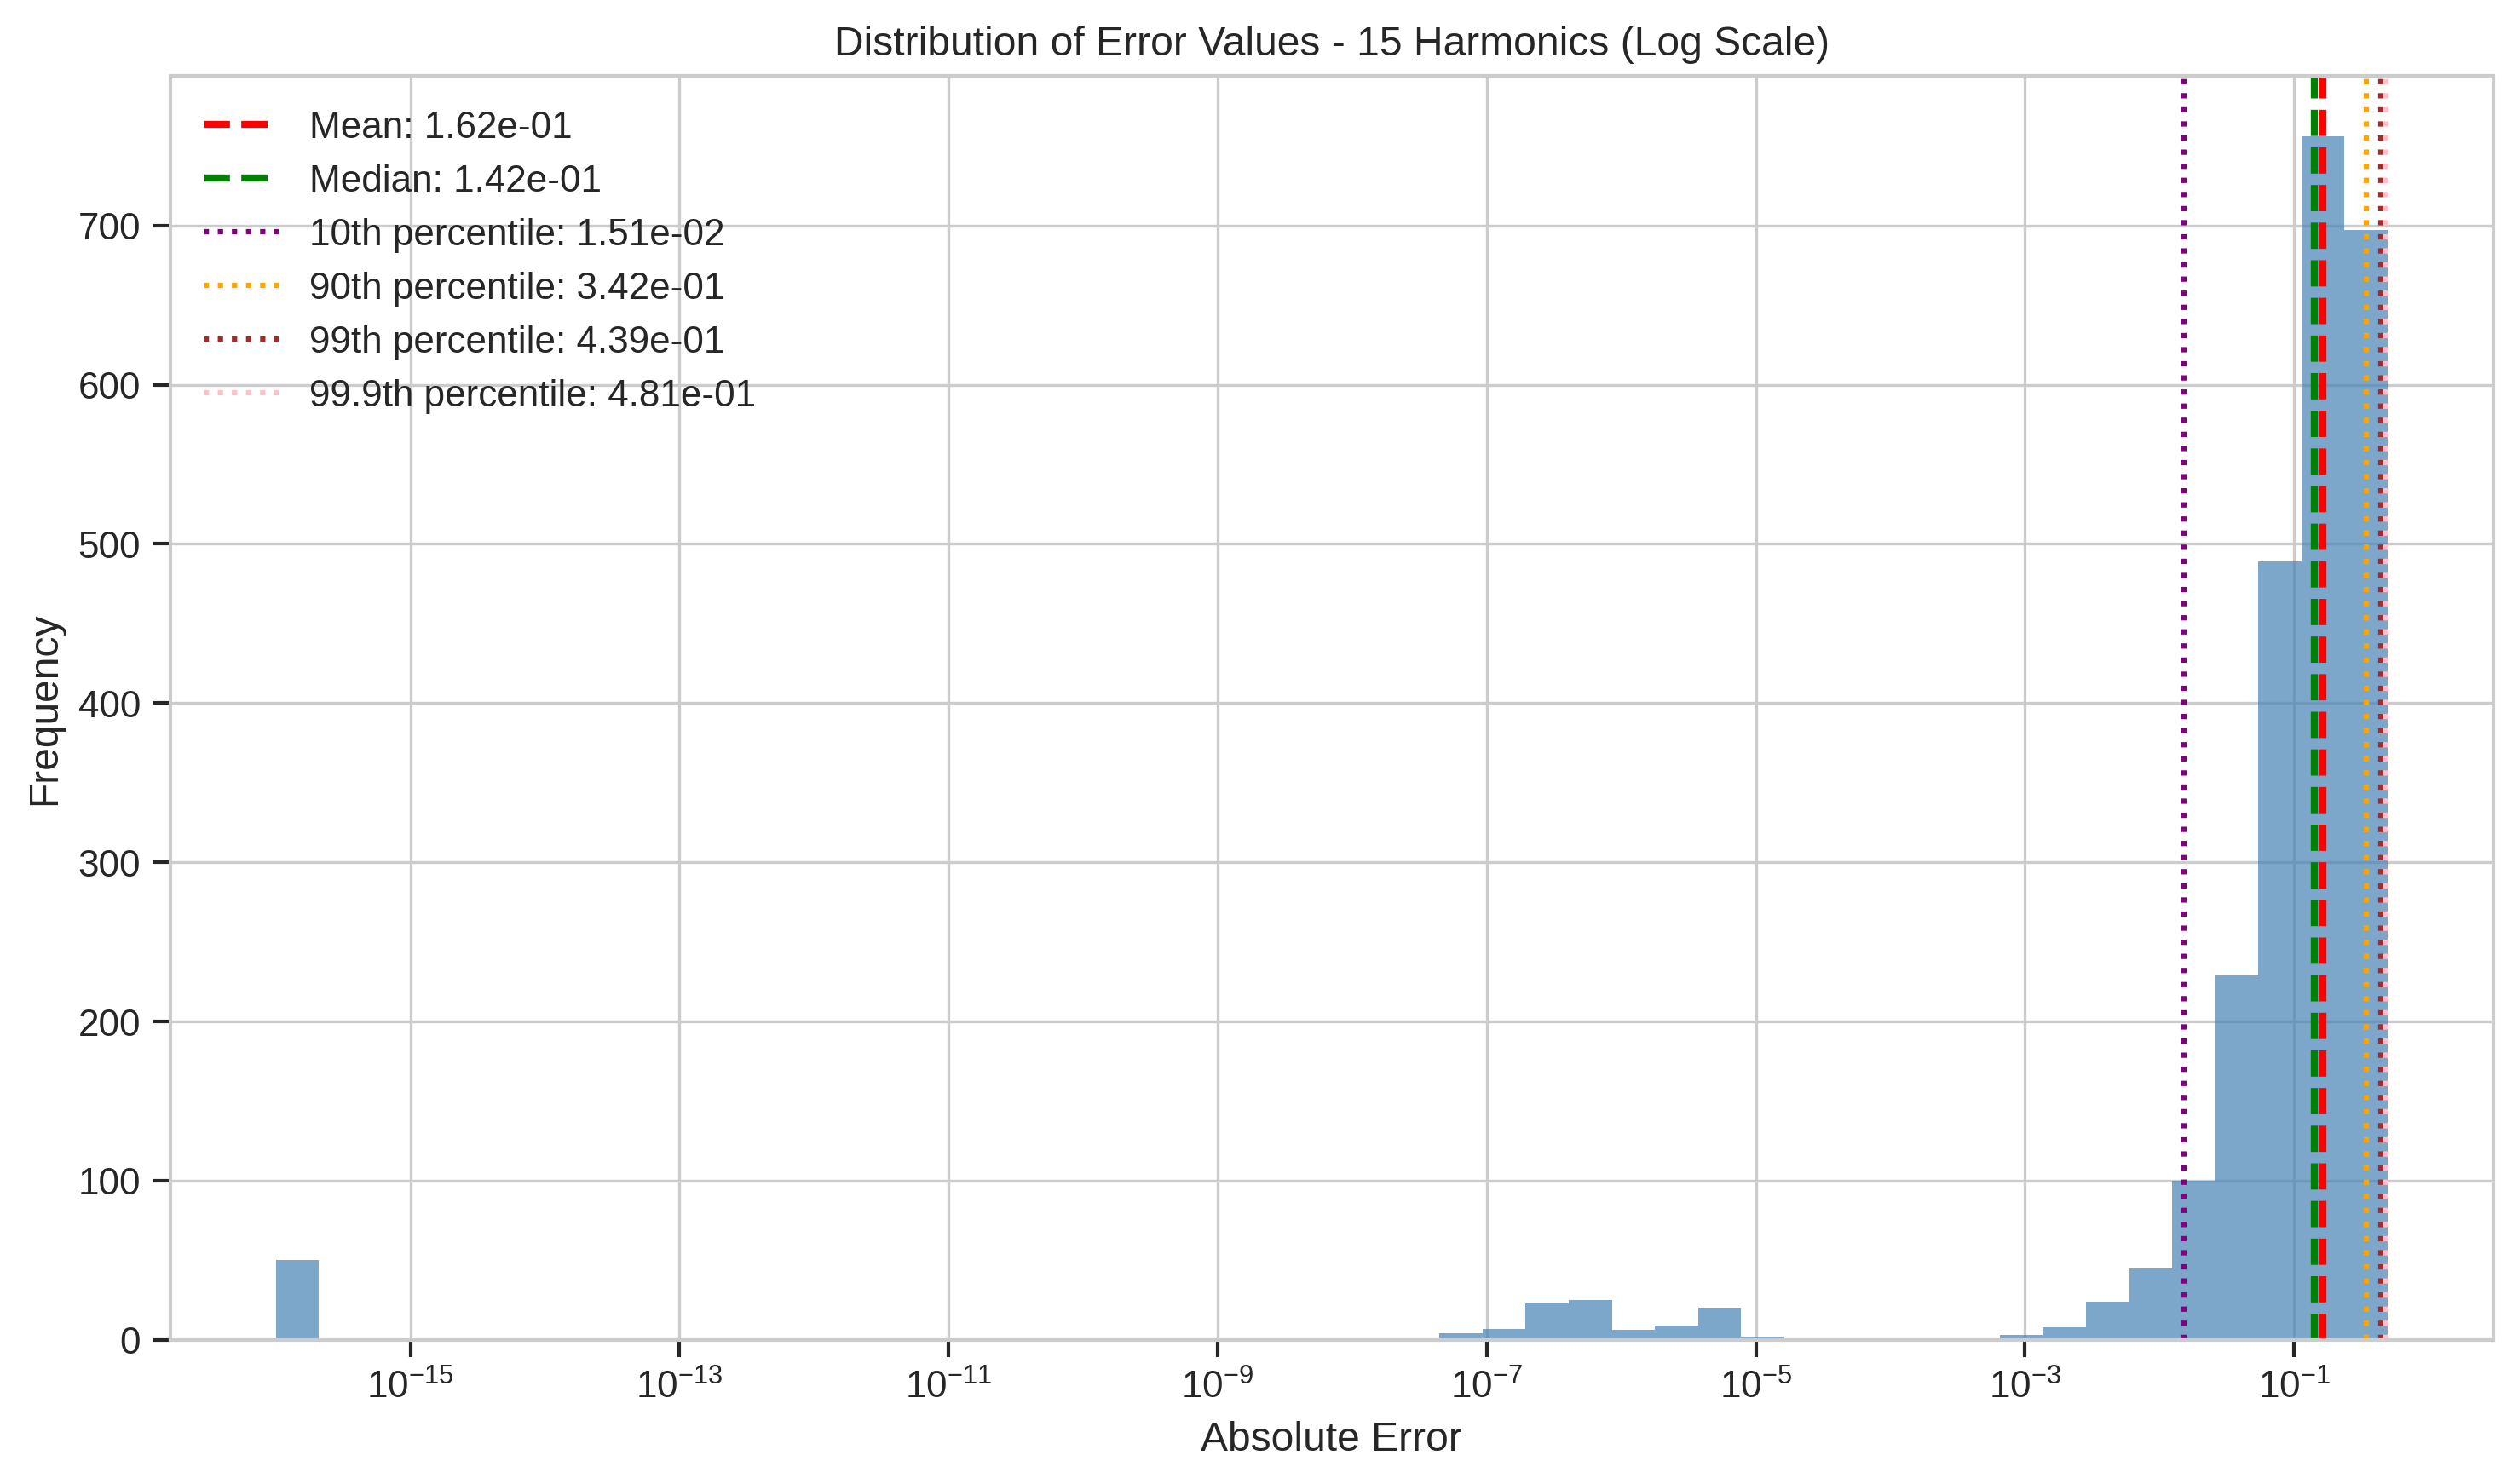
\includegraphics[width=\textwidth]{figures/error_distribution_15h.png}
        \caption{15 harmonics}
    \end{subfigure}
    \hfill
    \begin{subfigure}[b]{0.32\textwidth}
        \centering
        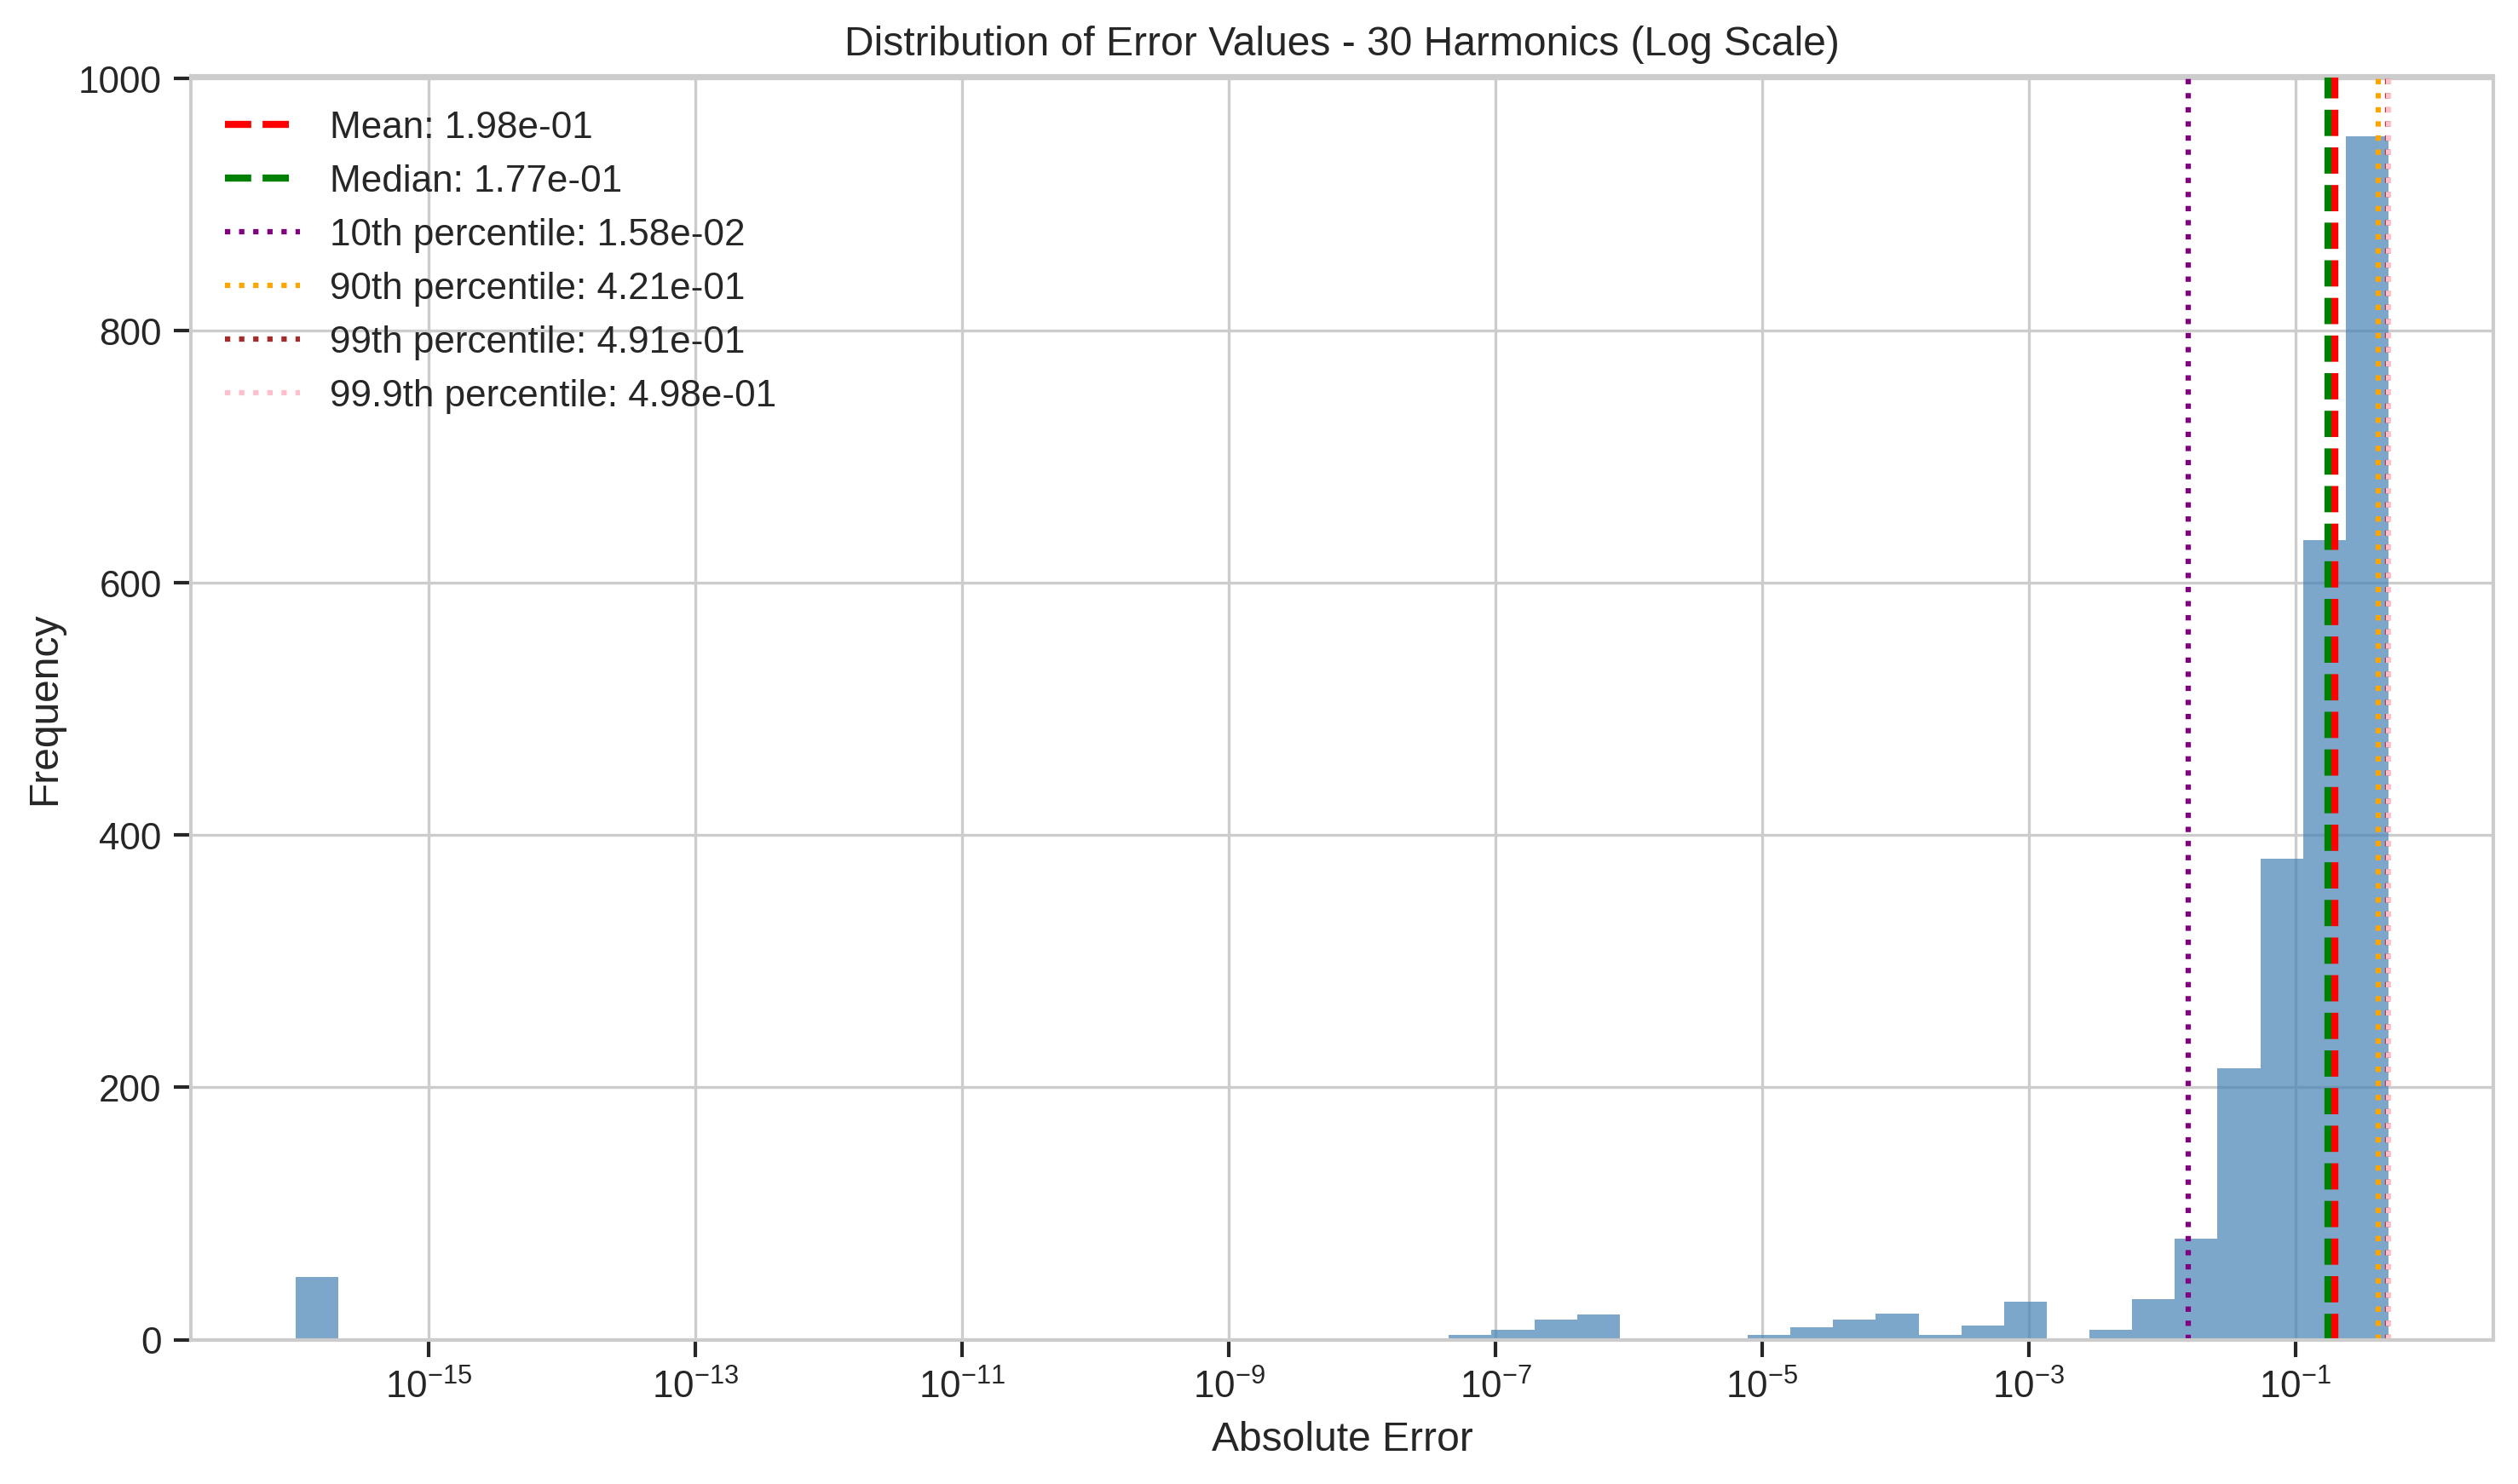
\includegraphics[width=\textwidth]{figures/error_distribution_30h.png}
        \caption{30 harmonics}
    \end{subfigure}
    \caption{Spatial error distributions for different harmonic configurations, revealing how error patterns change with model complexity.}
    \label{fig:error_dist_comparison}
\end{figure}

\subsection{Training Dynamics}

\begin{figure}[H]
    \centering
    \begin{subfigure}[b]{0.48\textwidth}
        \centering
        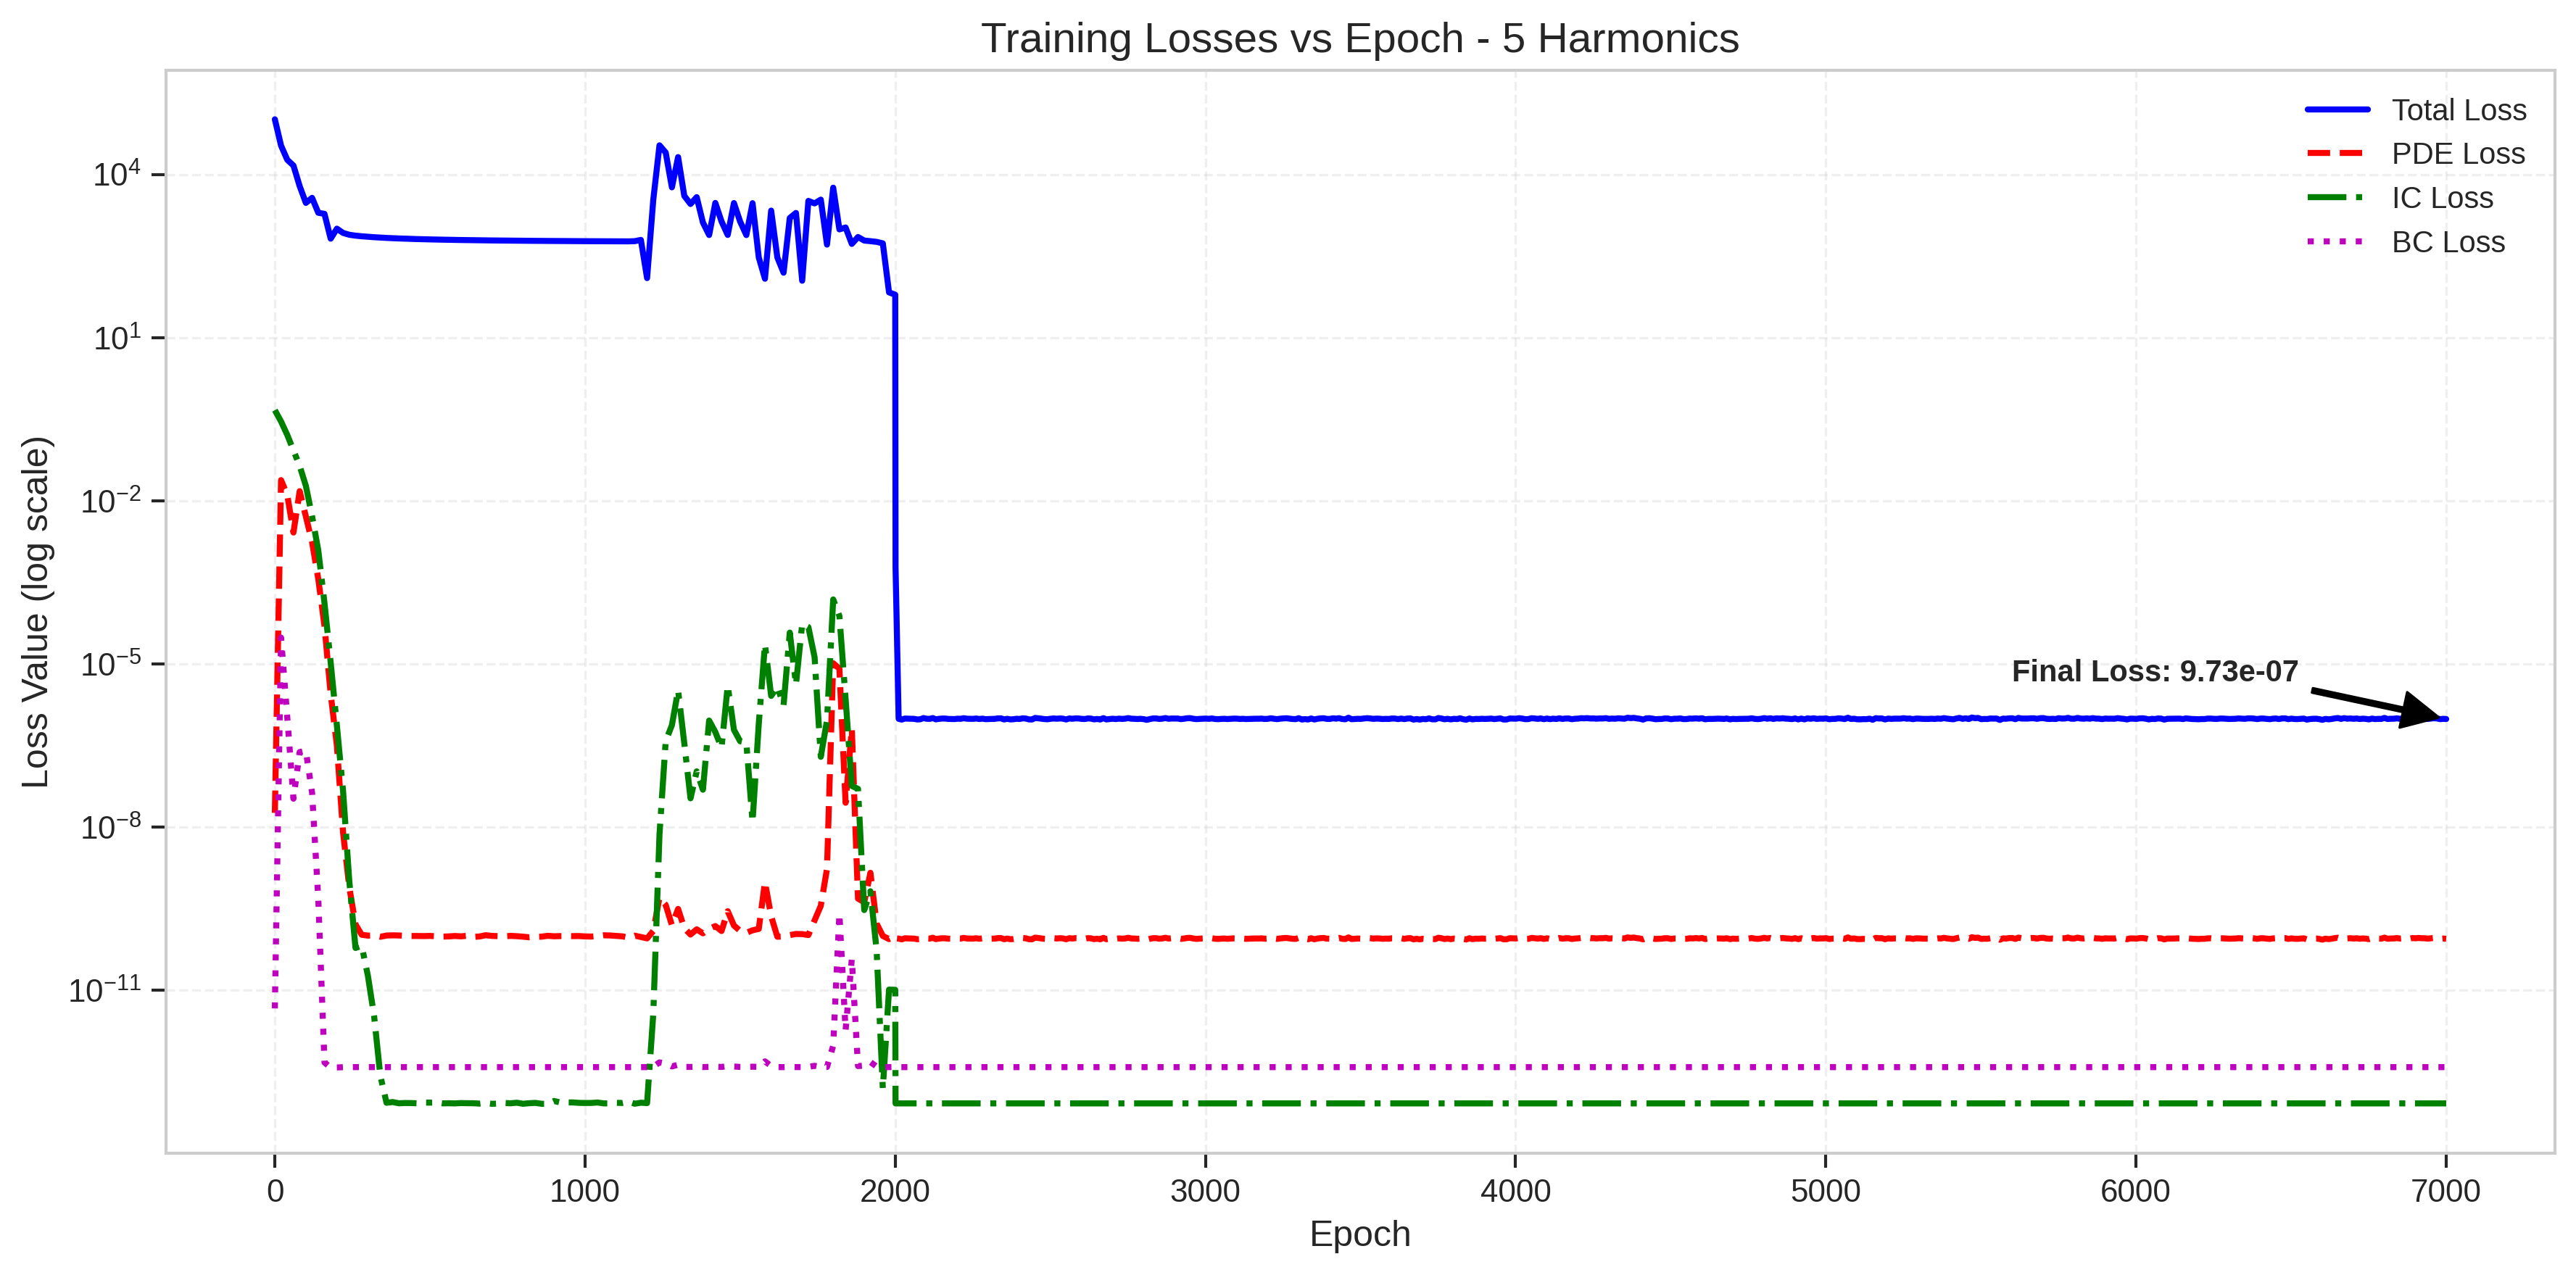
\includegraphics[width=\textwidth]{figures/training_losses_5h.png}
        \caption{5 harmonics training}
    \end{subfigure}
    \hfill
    \begin{subfigure}[b]{0.48\textwidth}
        \centering
        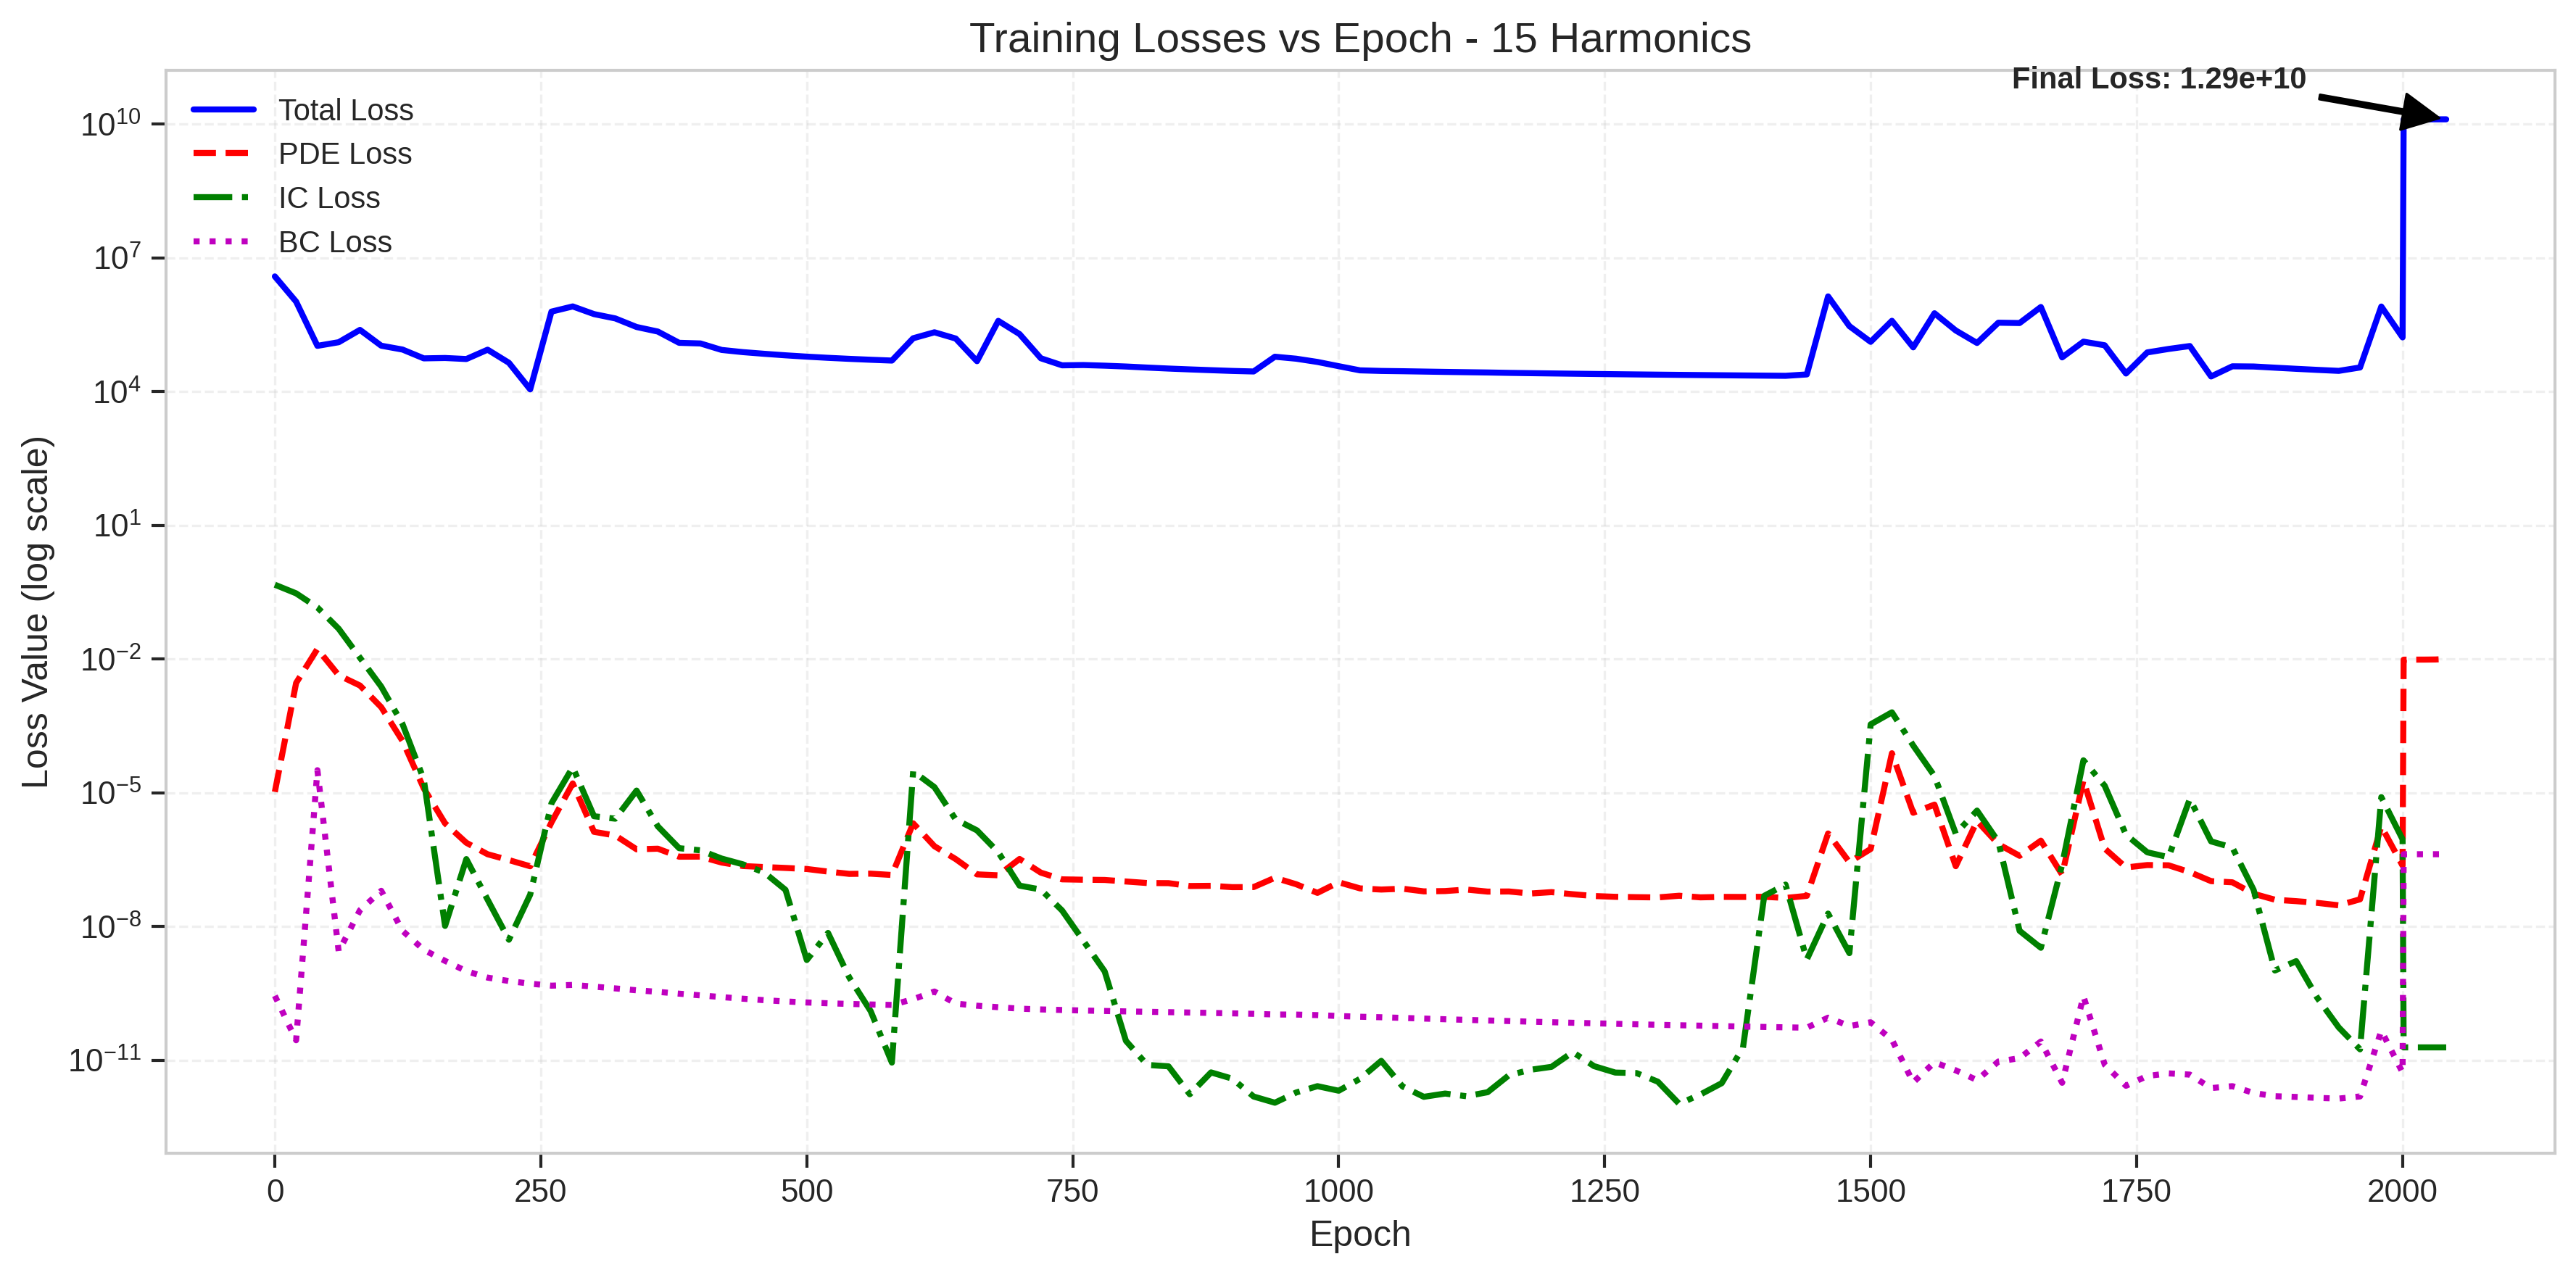
\includegraphics[width=\textwidth]{figures/training_losses_15h.png}
        \caption{15 harmonics training}
    \end{subfigure}
    \caption{Training loss evolution for suboptimal configurations, showing instabilities and convergence difficulties for higher harmonic counts.}
    \label{fig:training_comparison}
\end{figure}

\begin{figure}[H]
    \centering
    \begin{subfigure}[b]{0.48\textwidth}
        \centering
        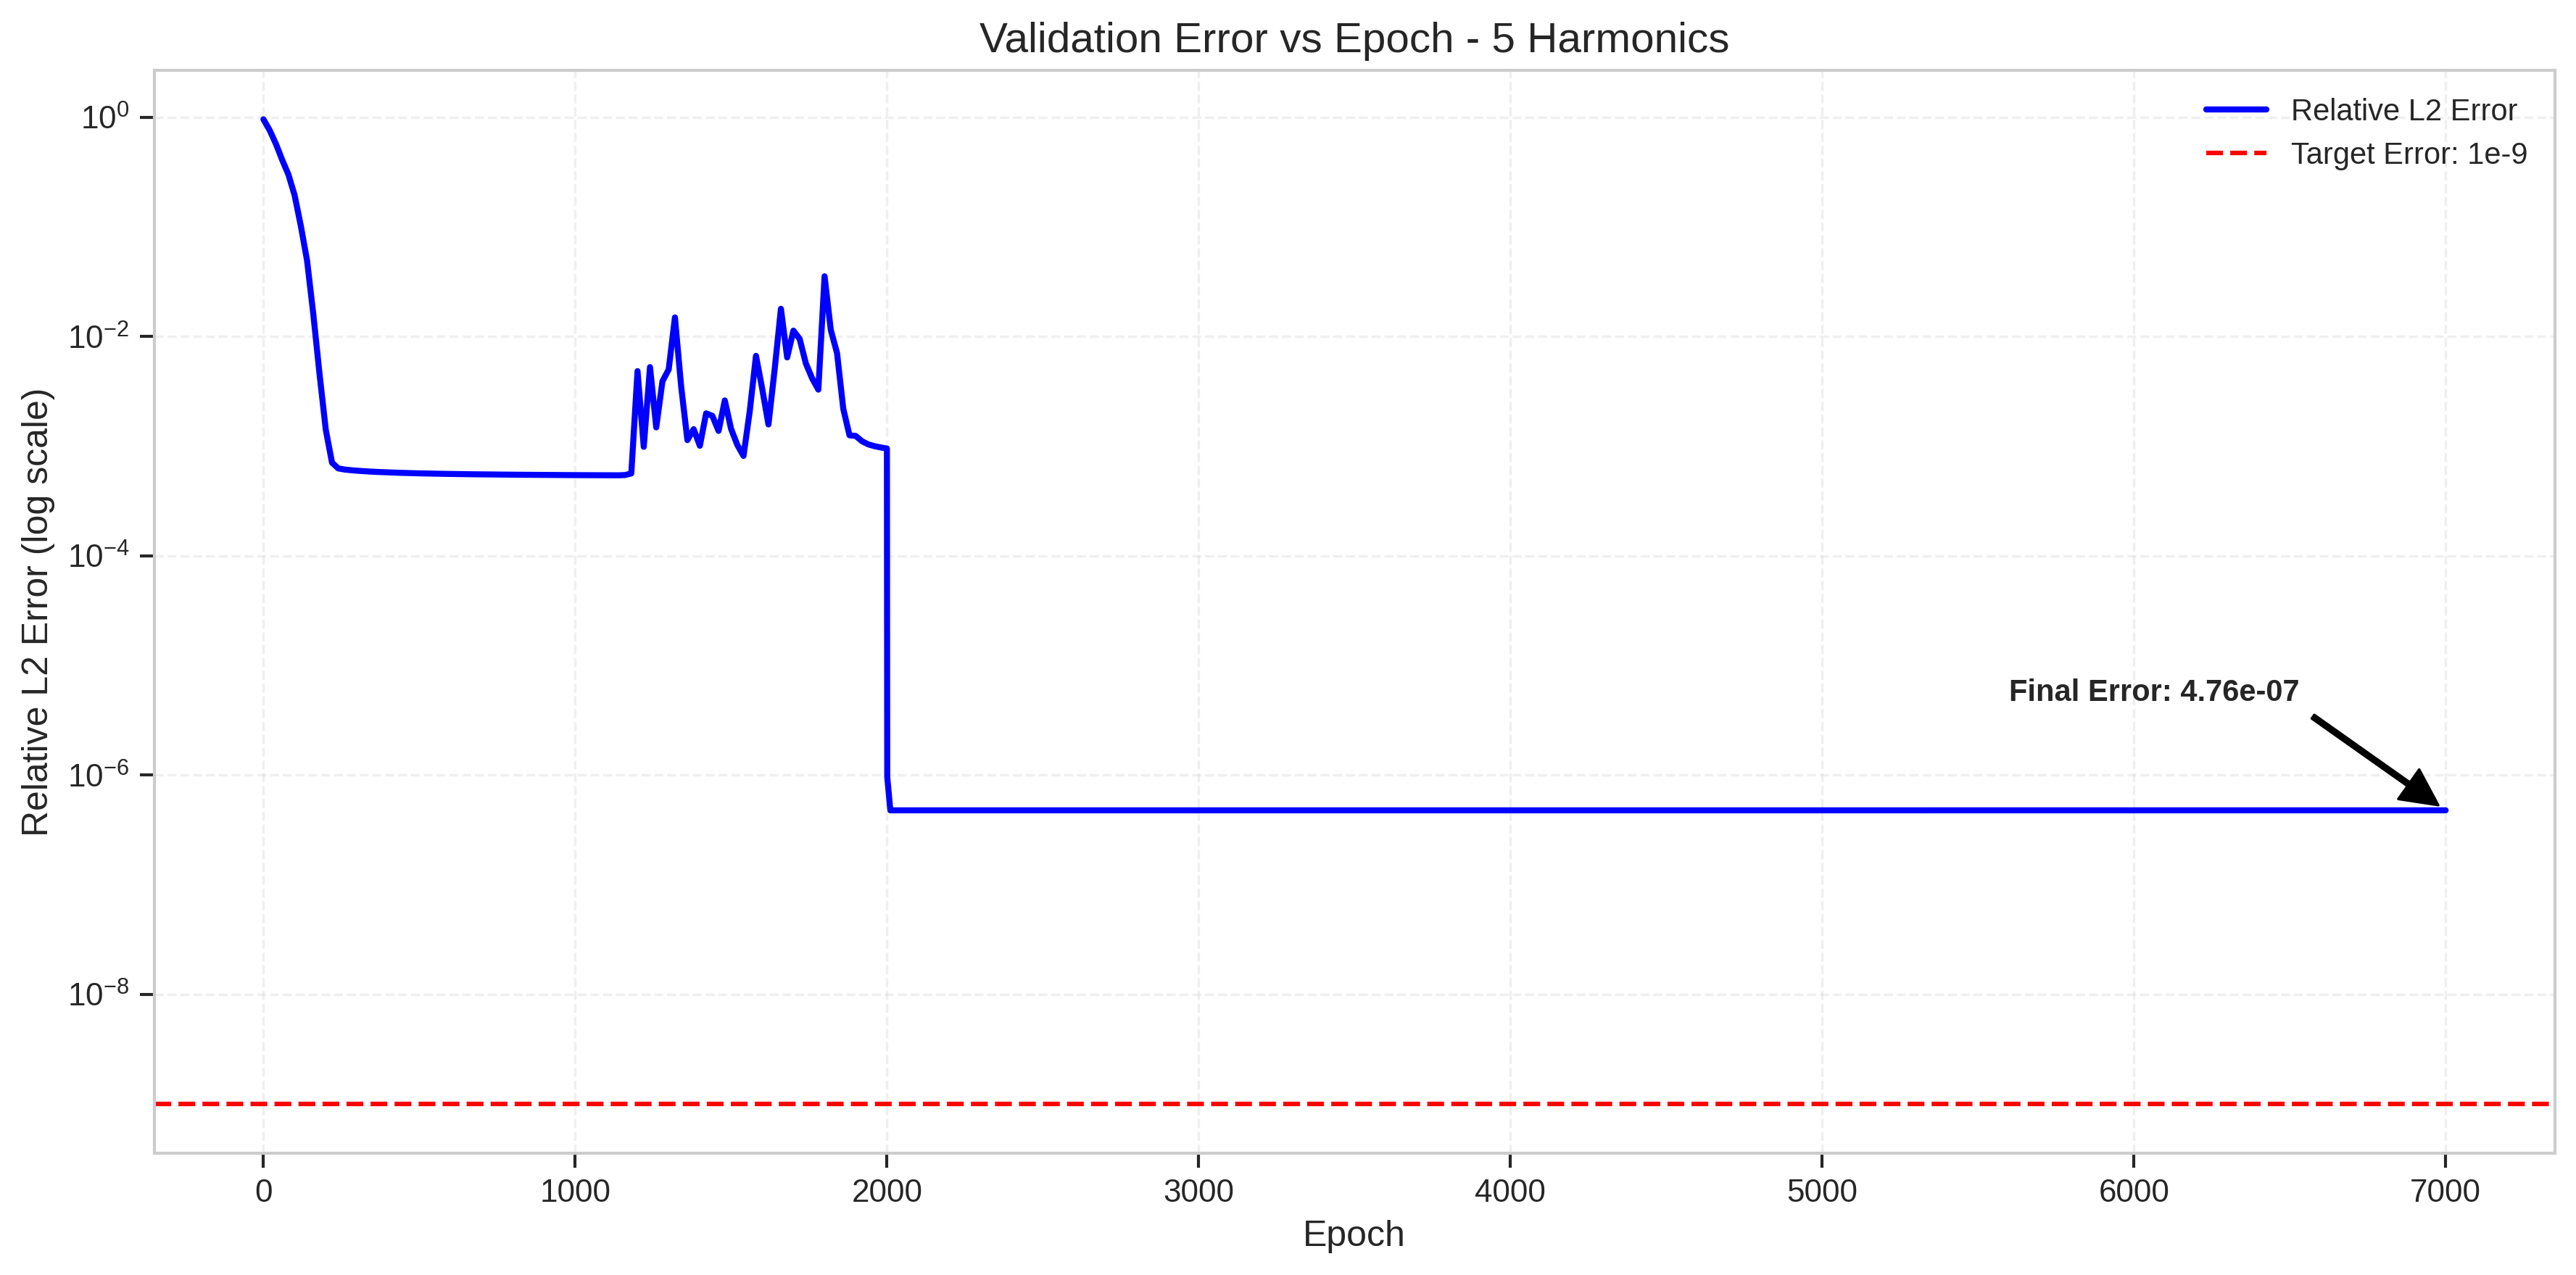
\includegraphics[width=\textwidth]{figures/validation_error_5h.png}
        \caption{5 harmonics validation}
    \end{subfigure}
    \hfill
    \begin{subfigure}[b]{0.48\textwidth}
        \centering
        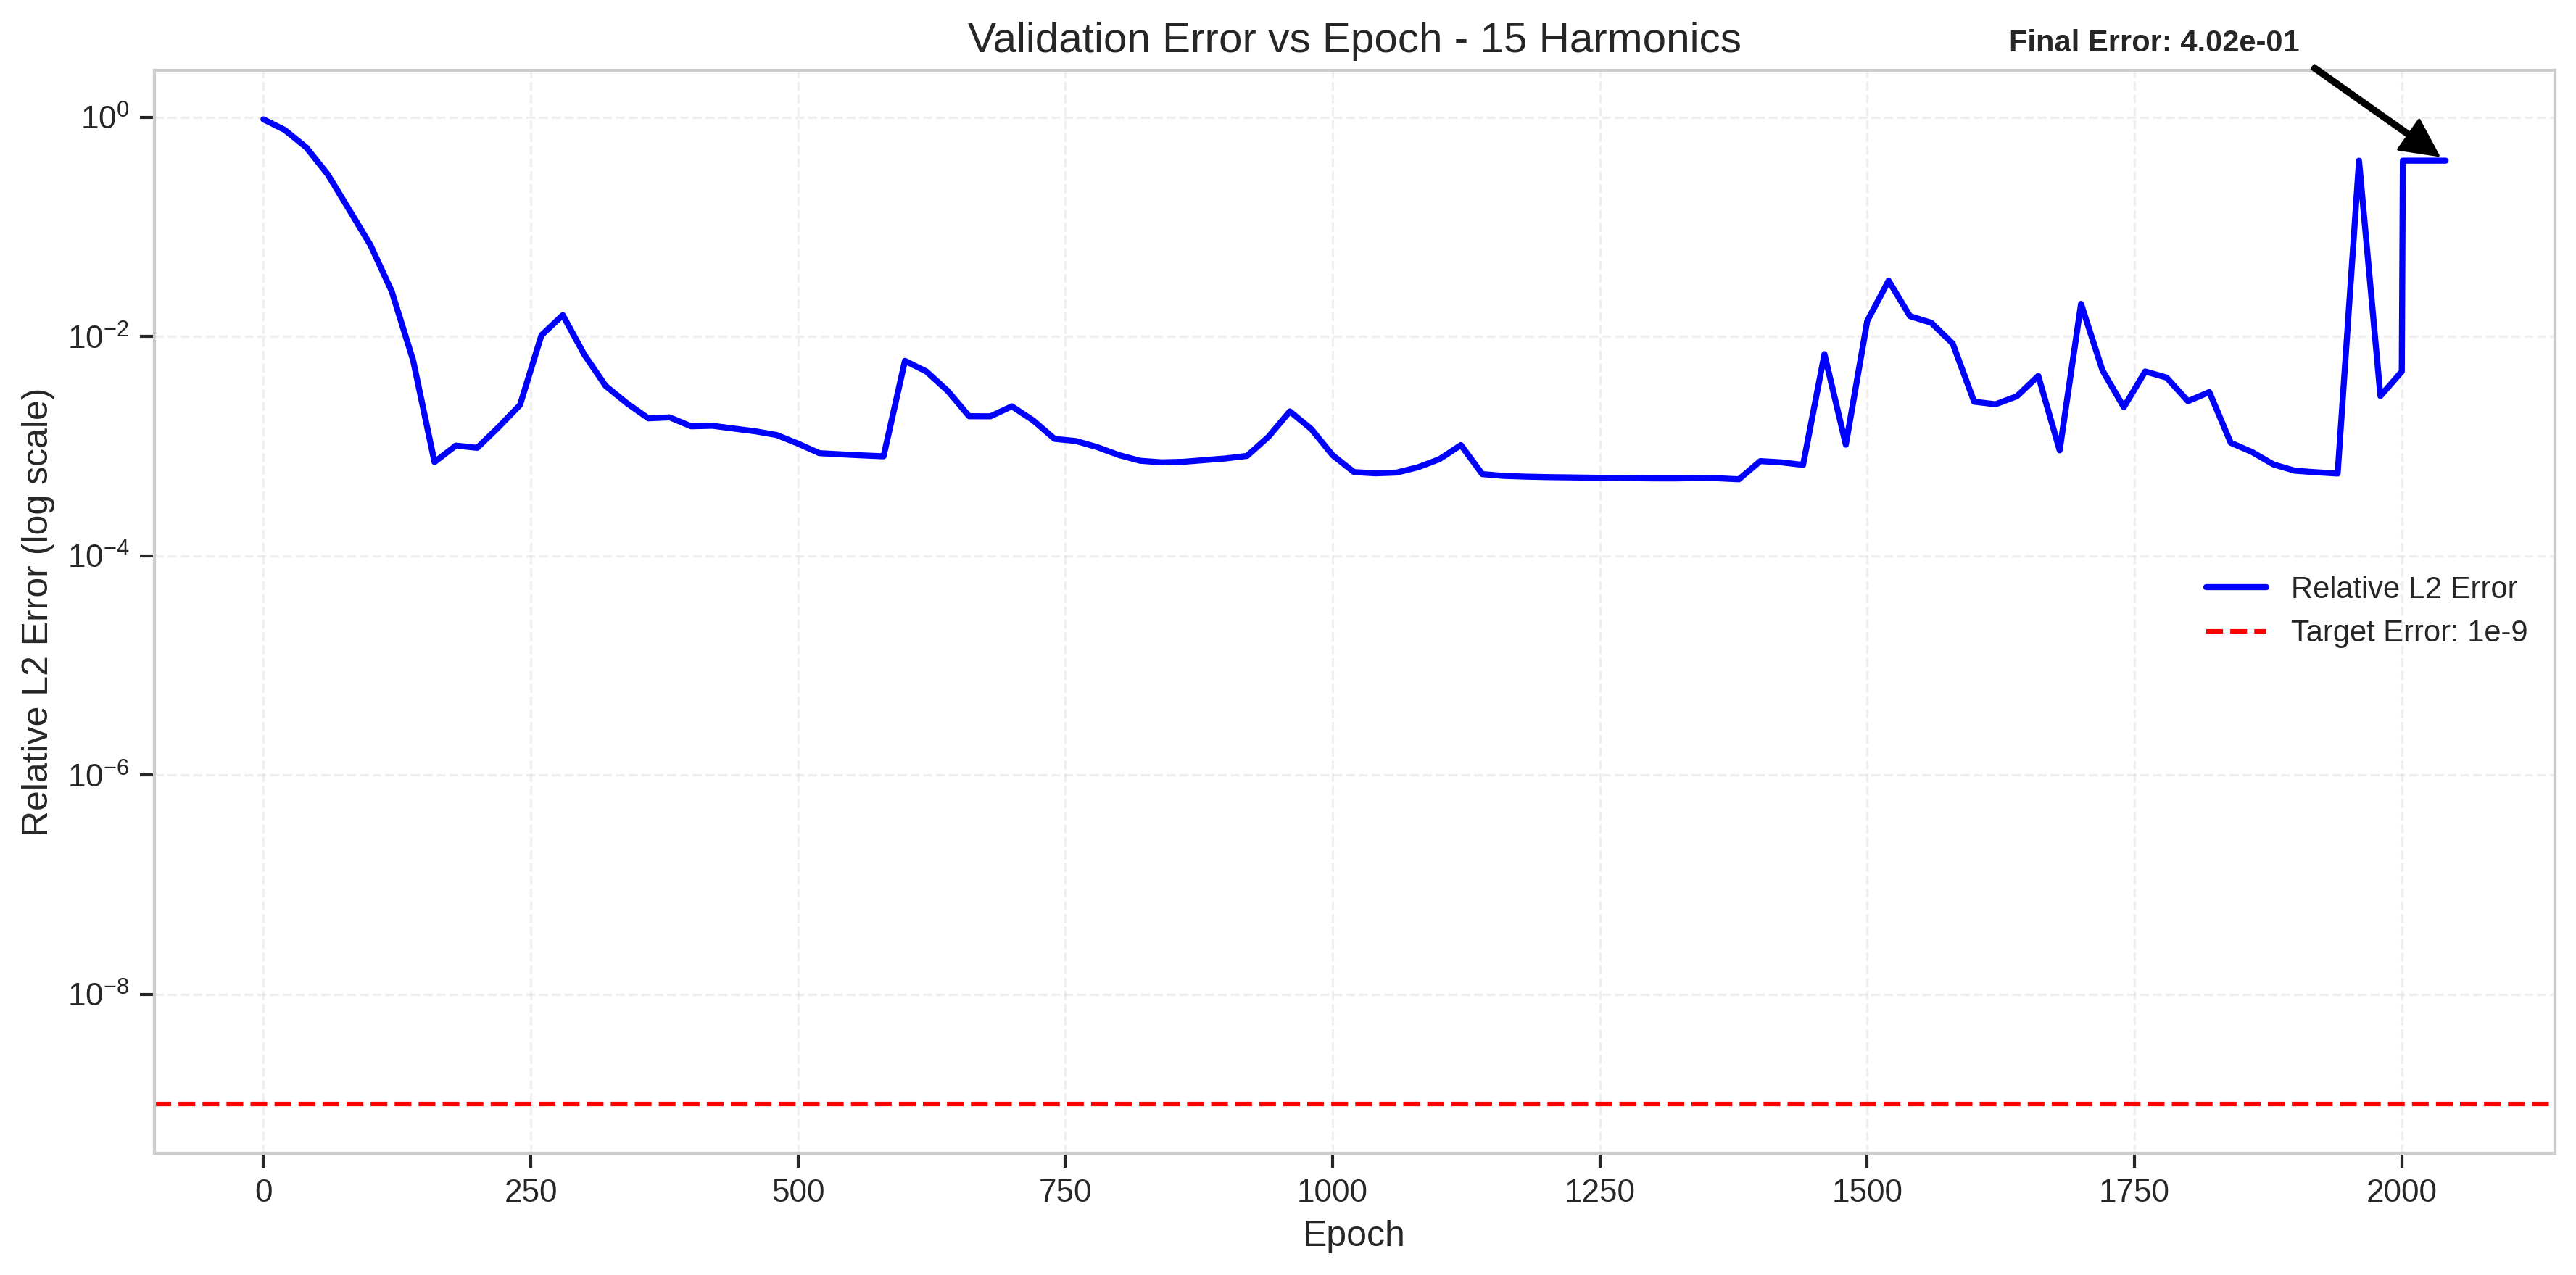
\includegraphics[width=\textwidth]{figures/validation_error_15h.png}
        \caption{15 harmonics validation}
    \end{subfigure}
    \caption{Validation error evolution demonstrating the generalization capabilities across different harmonic configurations.}
    \label{fig:validation_comparison}
\end{figure}

\subsection{Beam Deflection Analysis}

\begin{figure}[H]
    \centering
    \begin{subfigure}[b]{0.48\textwidth}
        \centering
        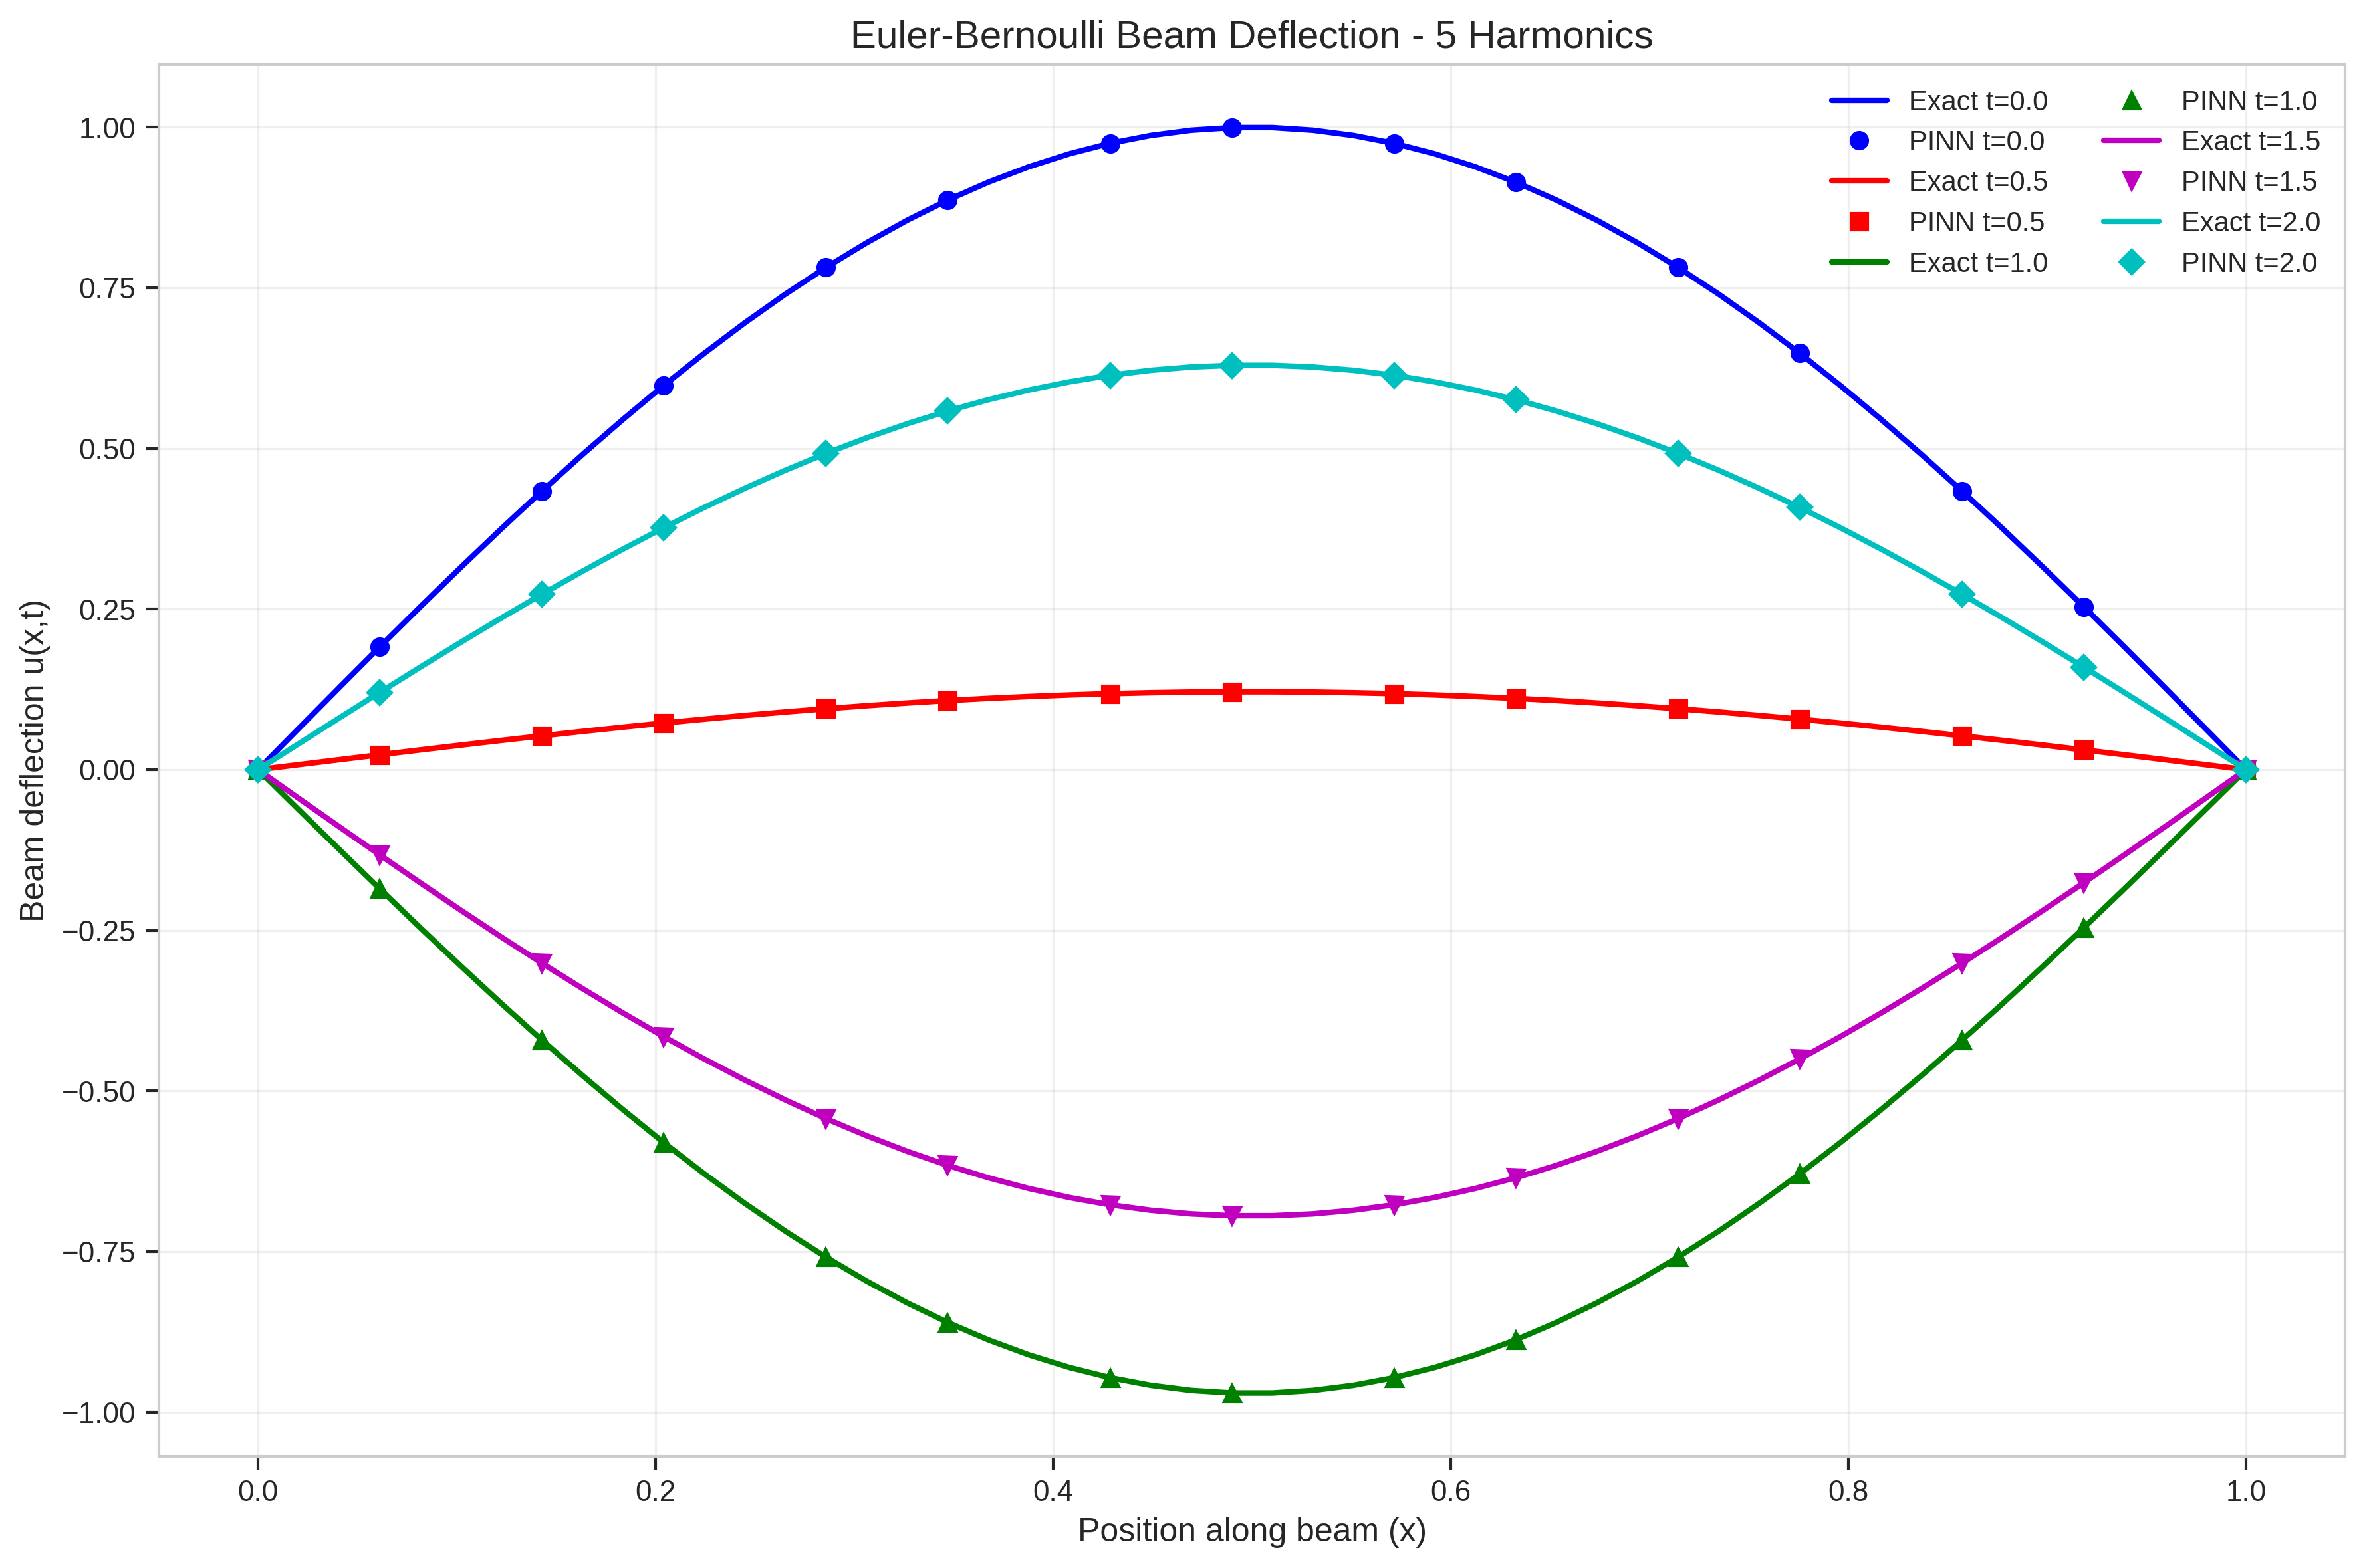
\includegraphics[width=\textwidth]{figures/euler_bernoulli_beam_5h.png}
        \caption{5 harmonics}
    \end{subfigure}
    \hfill
    \begin{subfigure}[b]{0.48\textwidth}
        \centering
        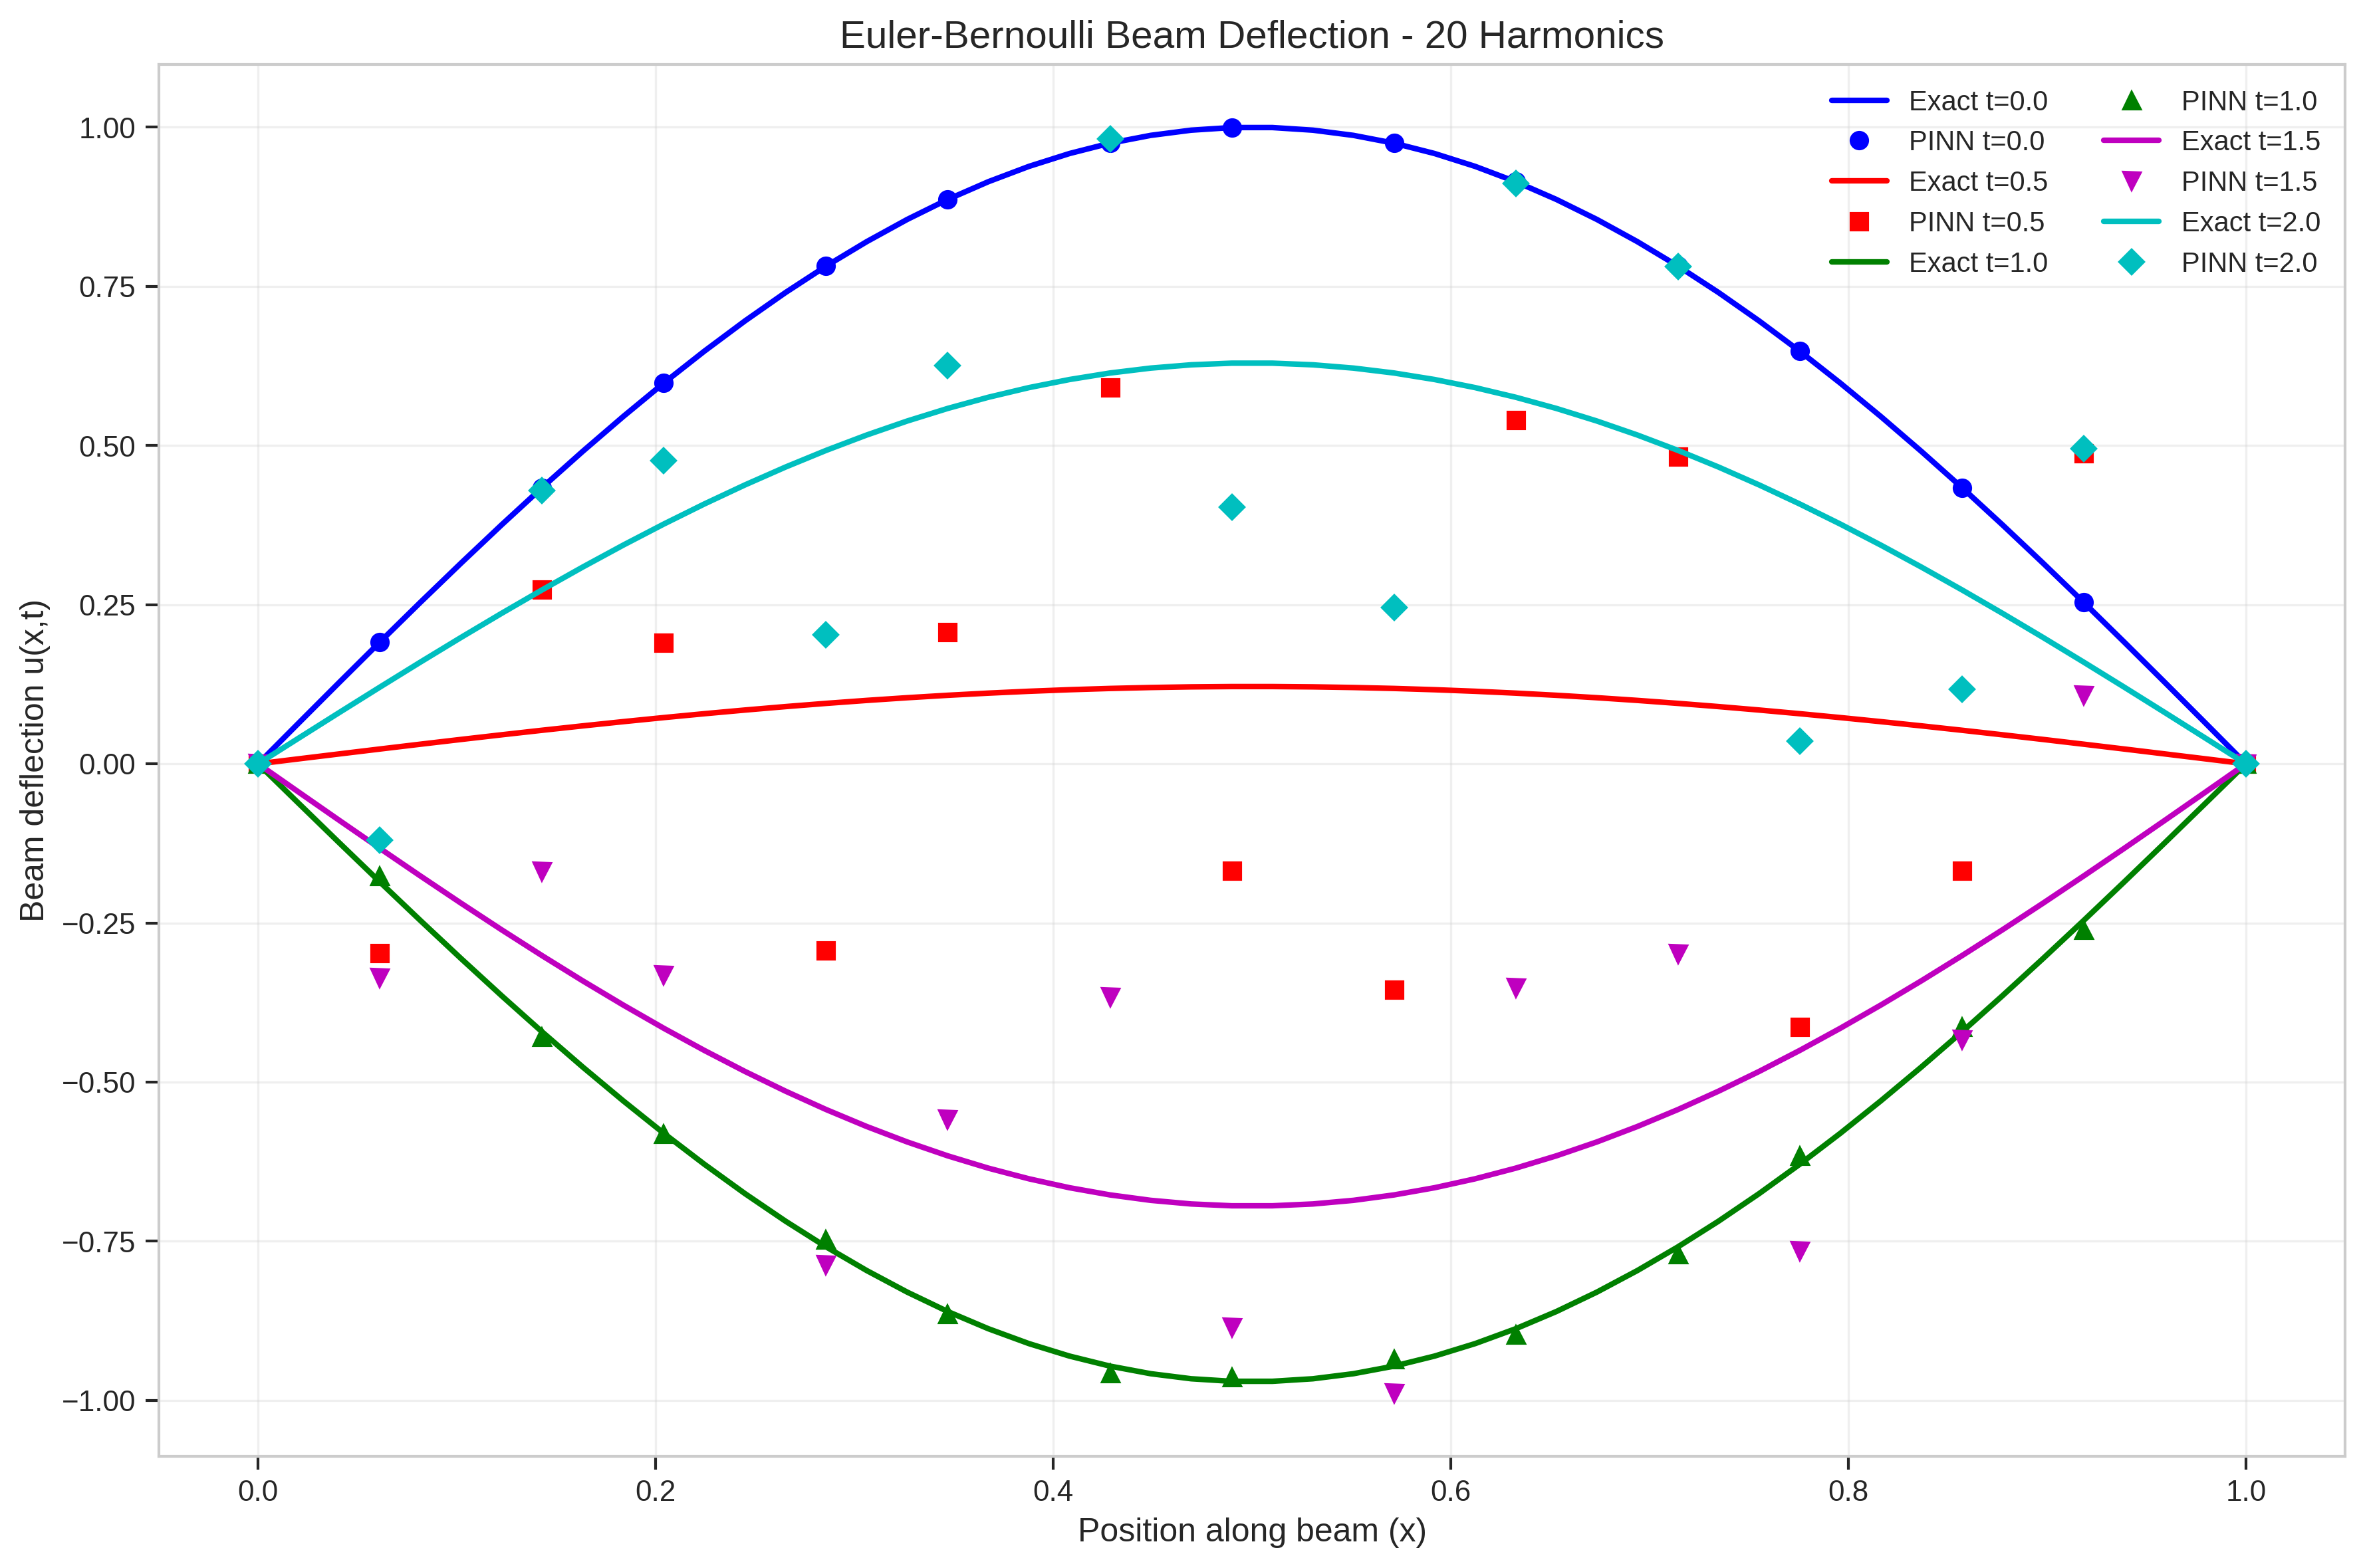
\includegraphics[width=\textwidth]{figures/euler_bernoulli_beam_20h.png}
        \caption{20 harmonics}
    \end{subfigure}
    \caption{Euler-Bernoulli beam deflection profiles at different time instances, comparing low and moderate harmonic configurations.}
    \label{fig:beam_comparison}
\end{figure}

\begin{figure}[H]
    \centering
    \begin{subfigure}[b]{0.48\textwidth}
        \centering
        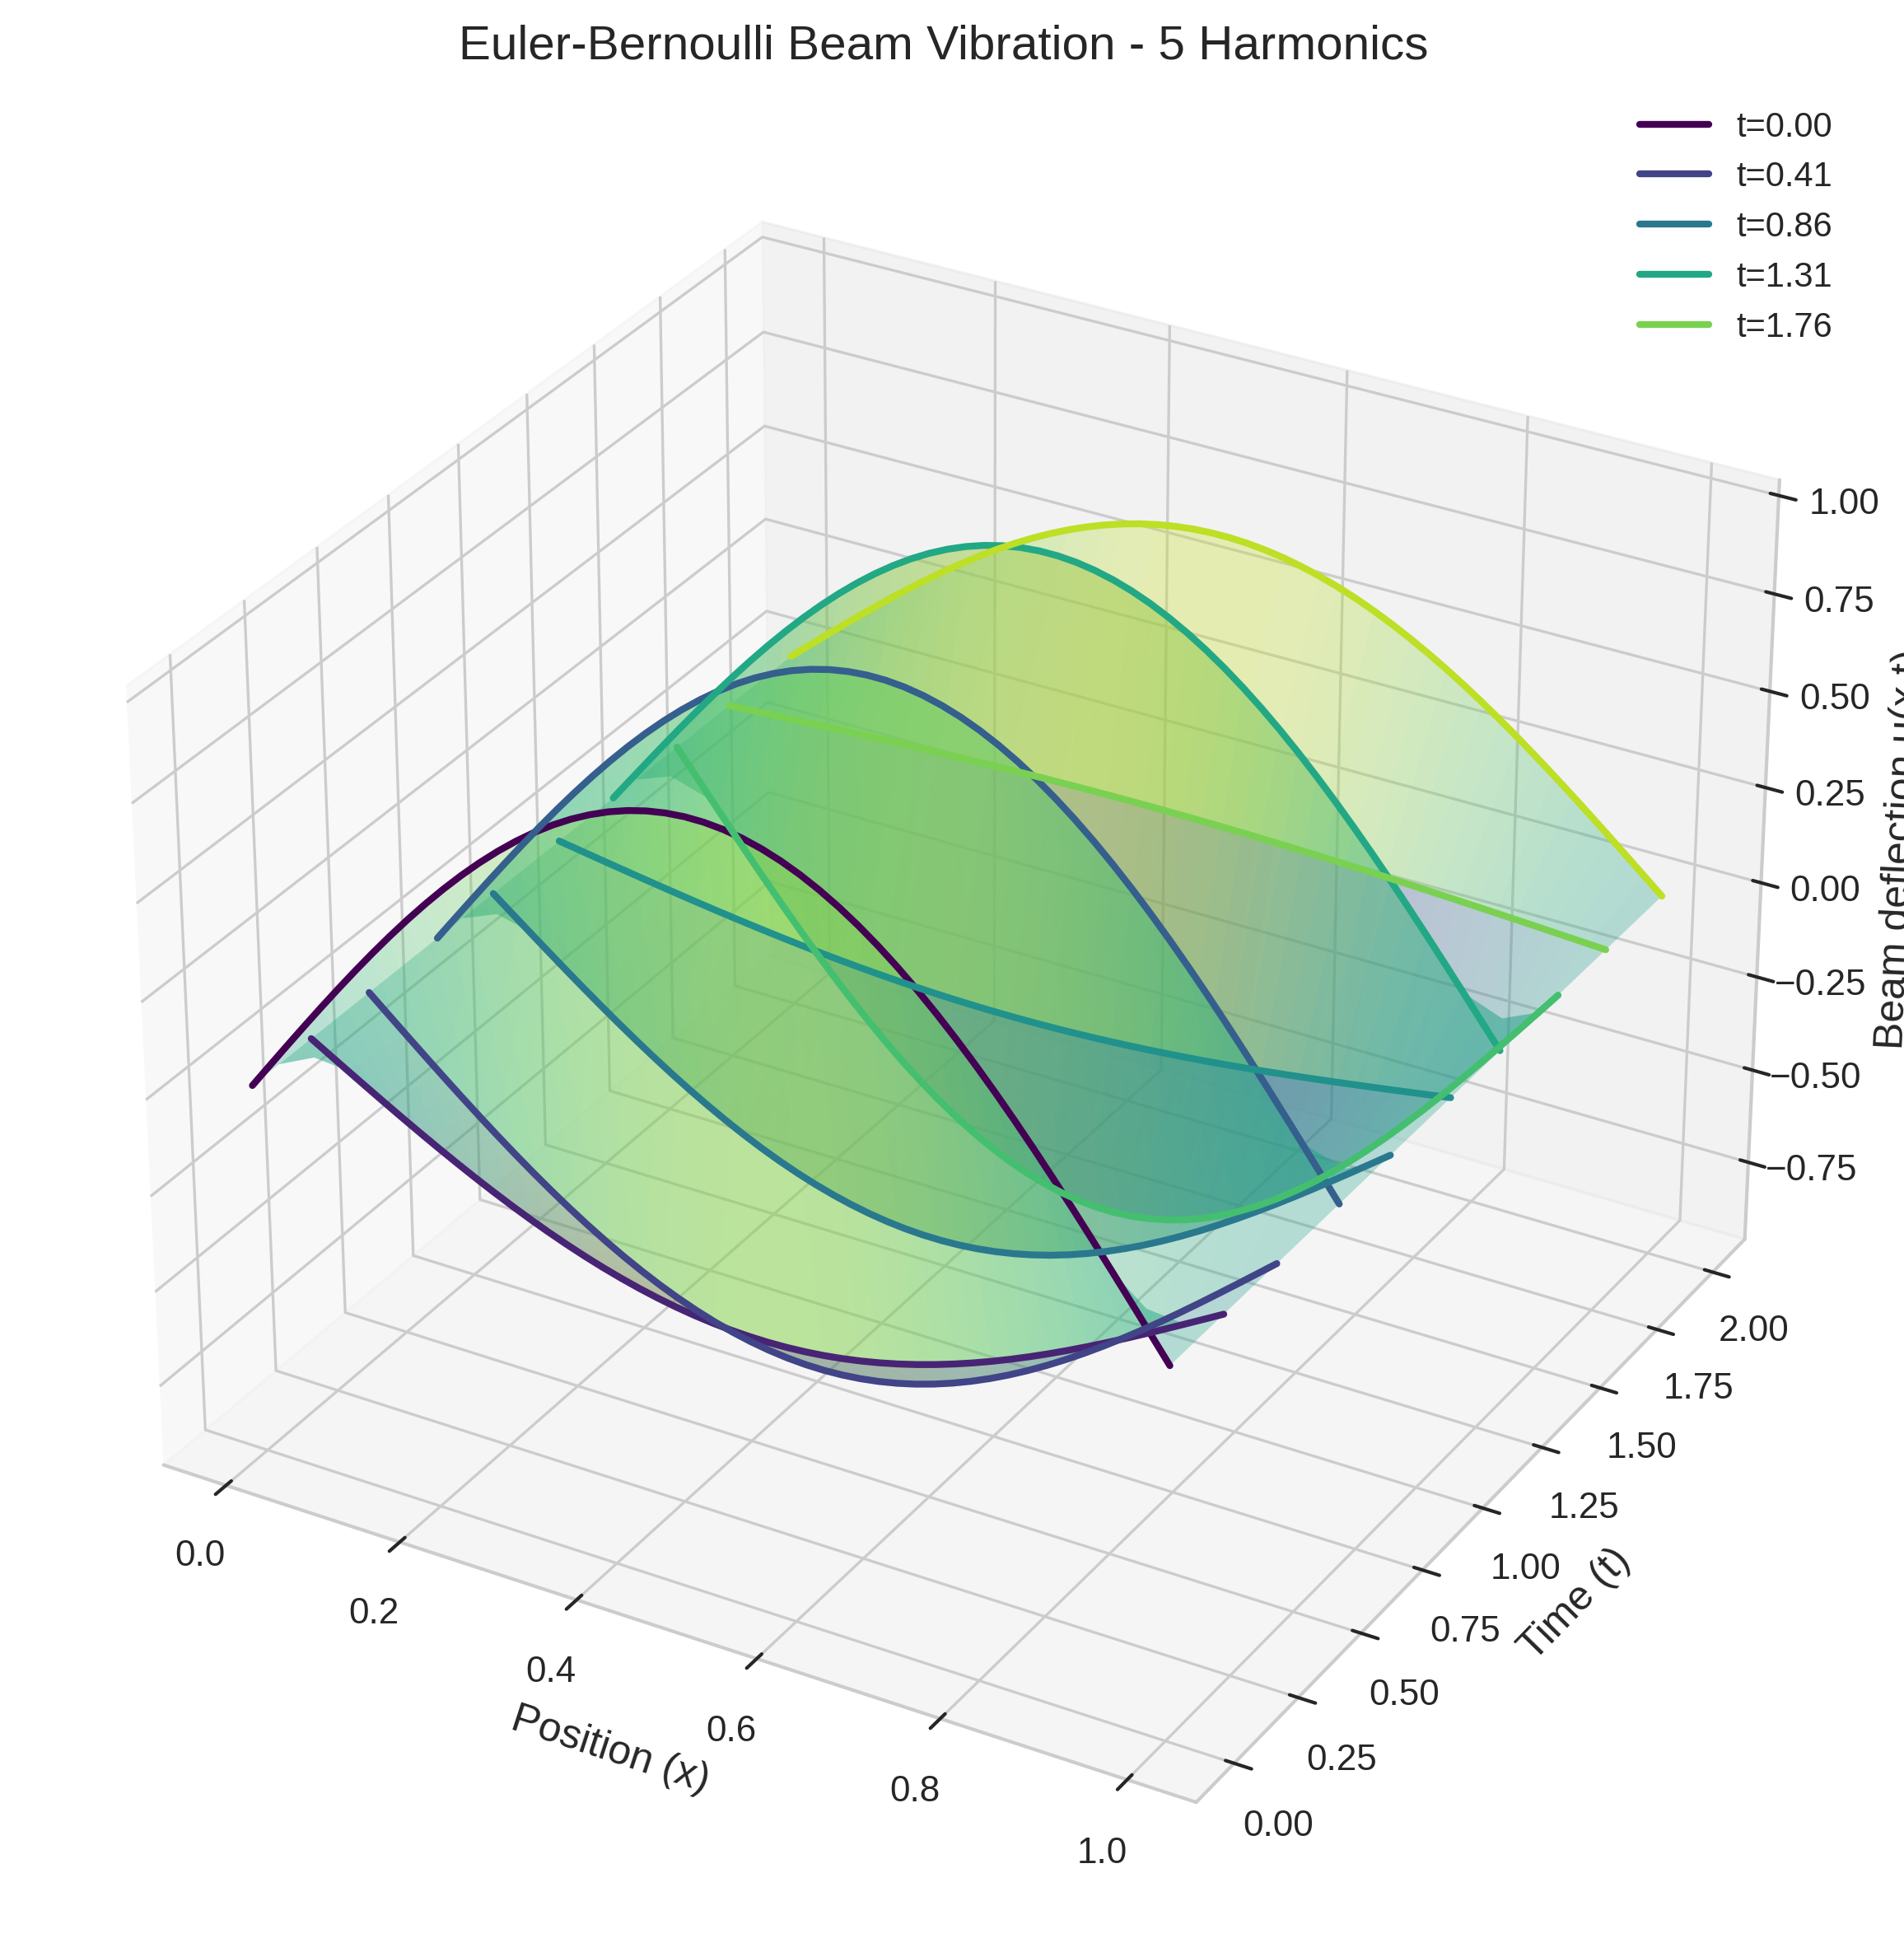
\includegraphics[width=\textwidth]{figures/euler_bernoulli_3d_5h.png}
        \caption{5 harmonics 3D view}
    \end{subfigure}
    \hfill
    \begin{subfigure}[b]{0.48\textwidth}
        \centering
        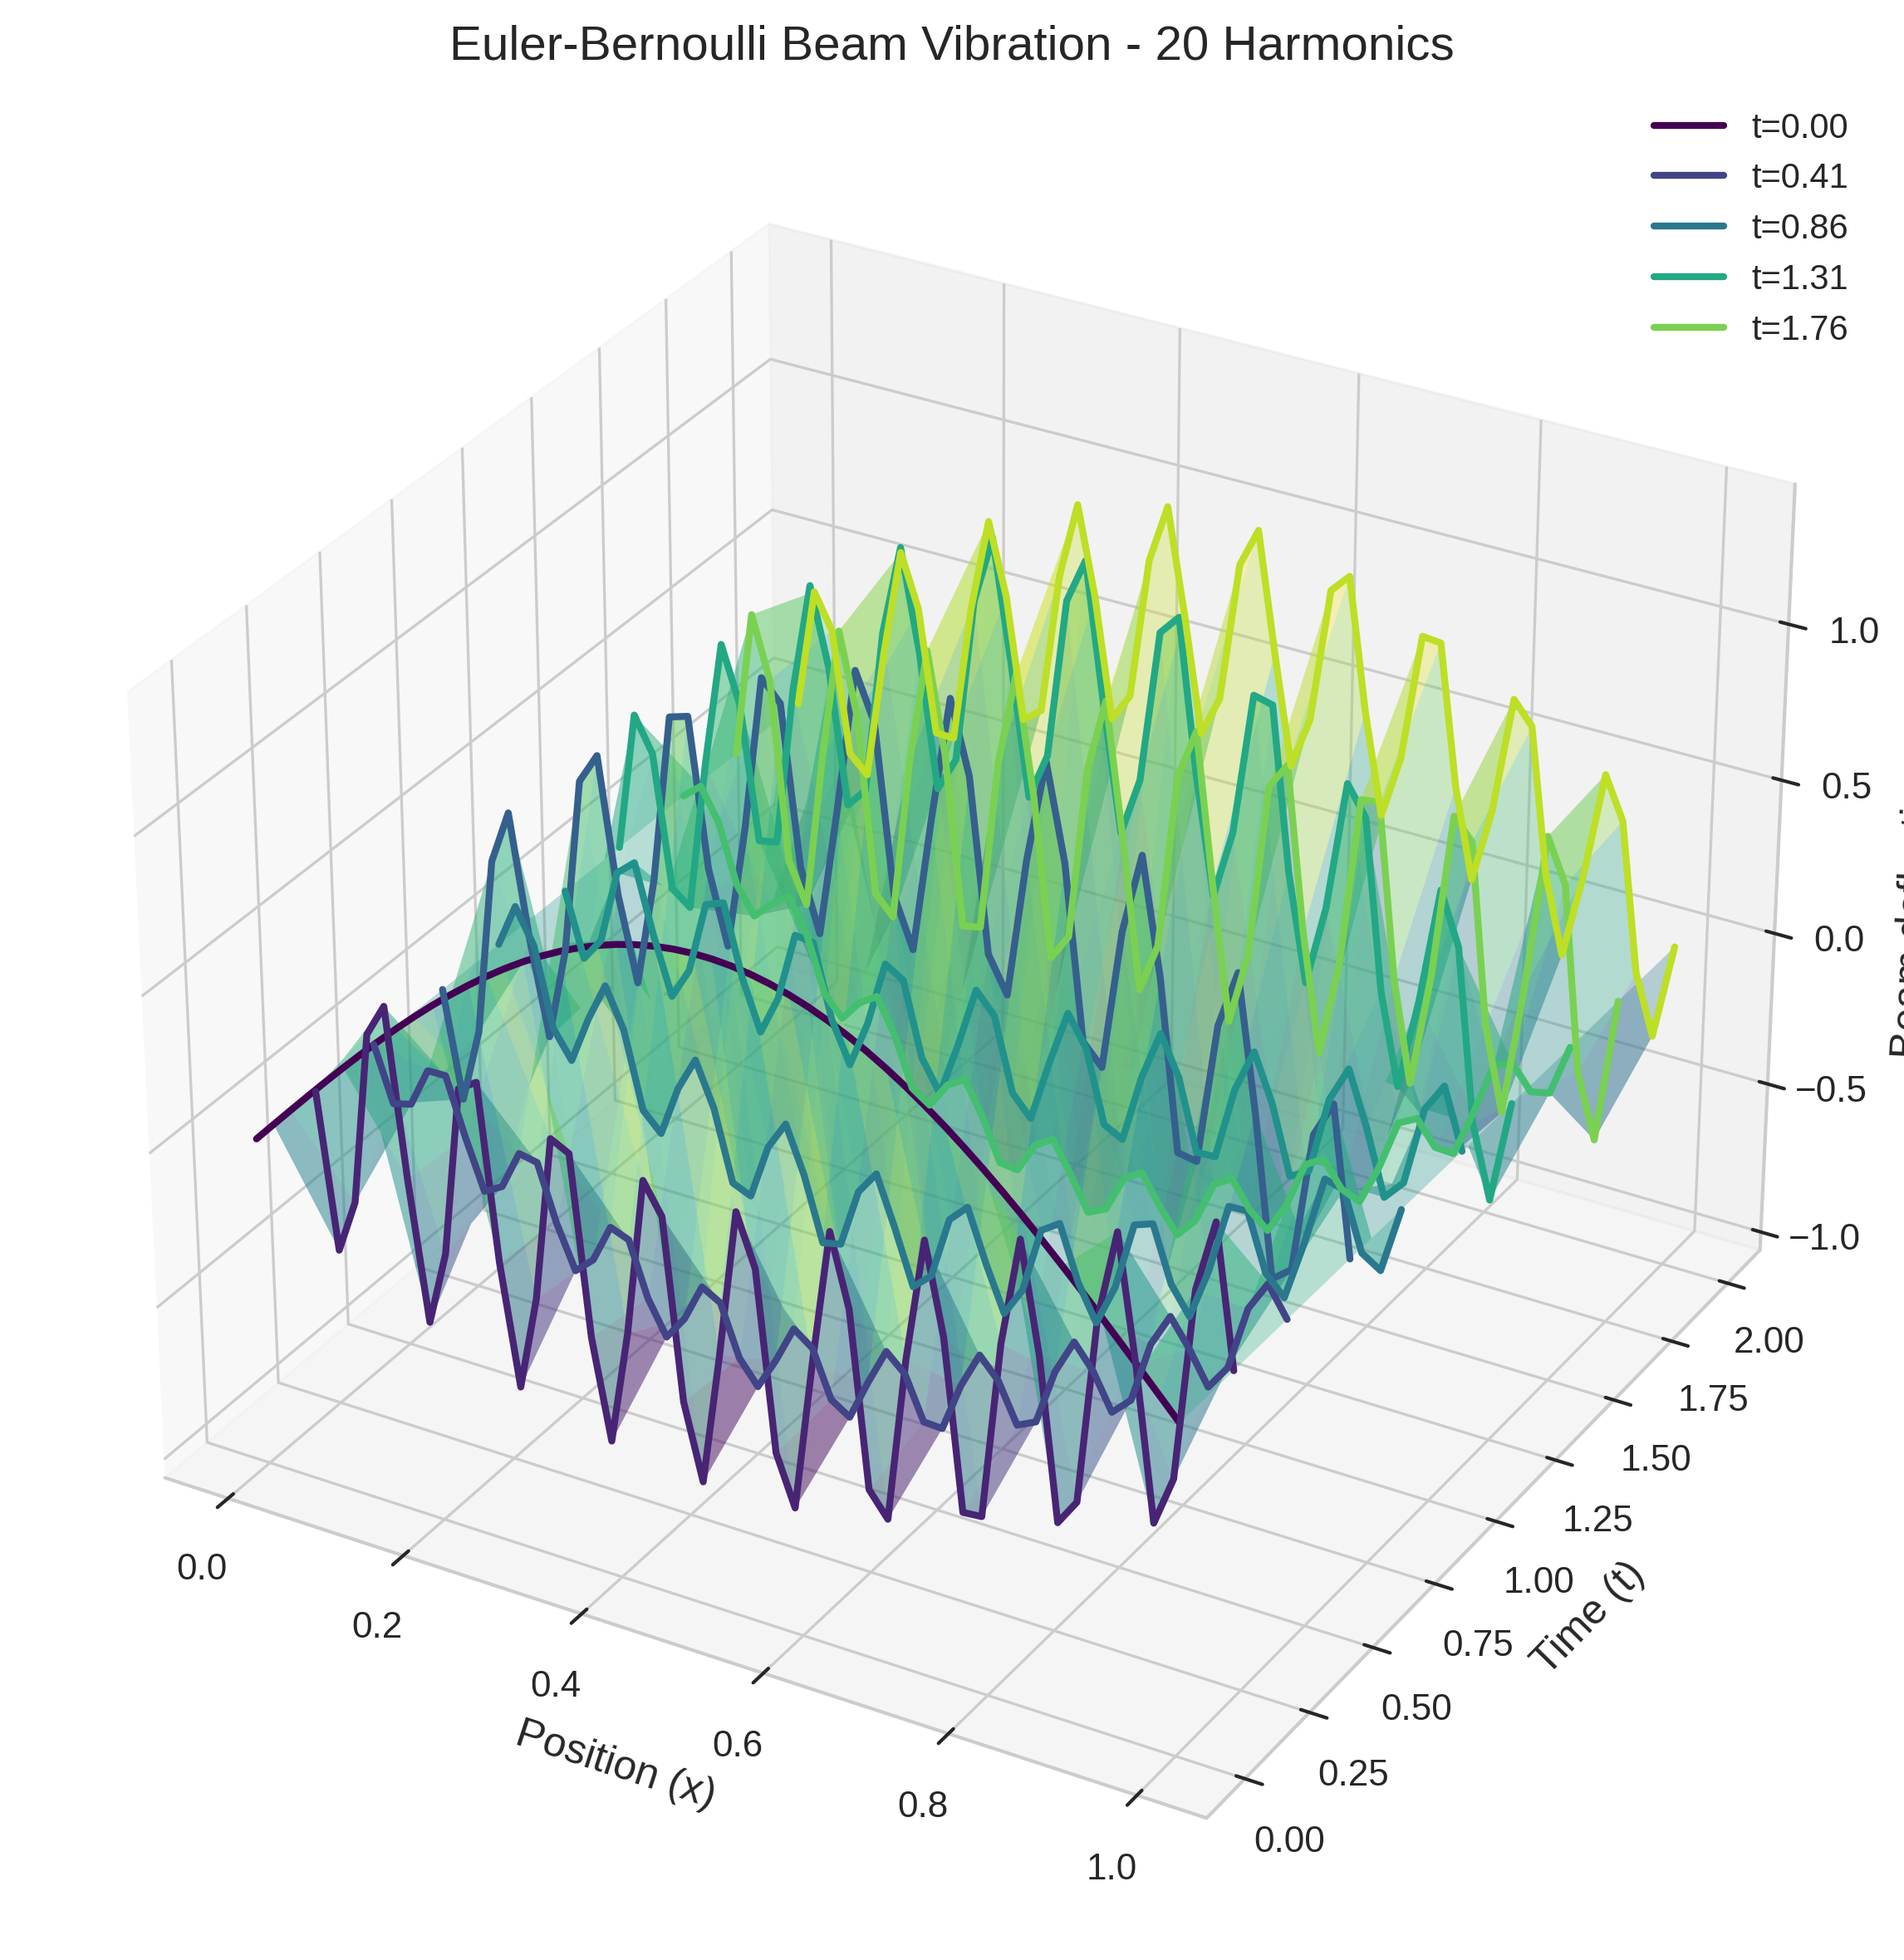
\includegraphics[width=\textwidth]{figures/euler_bernoulli_3d_20h.png}
        \caption{20 harmonics 3D view}
    \end{subfigure}
    \caption{Three-dimensional beam vibration patterns showing the spatiotemporal evolution for different harmonic configurations.}
    \label{fig:beam_3d_comparison}
\end{figure}

\subsection{Adaptive Weight Evolution}

\begin{figure}[H]
    \centering
    \begin{subfigure}[b]{0.48\textwidth}
        \centering
        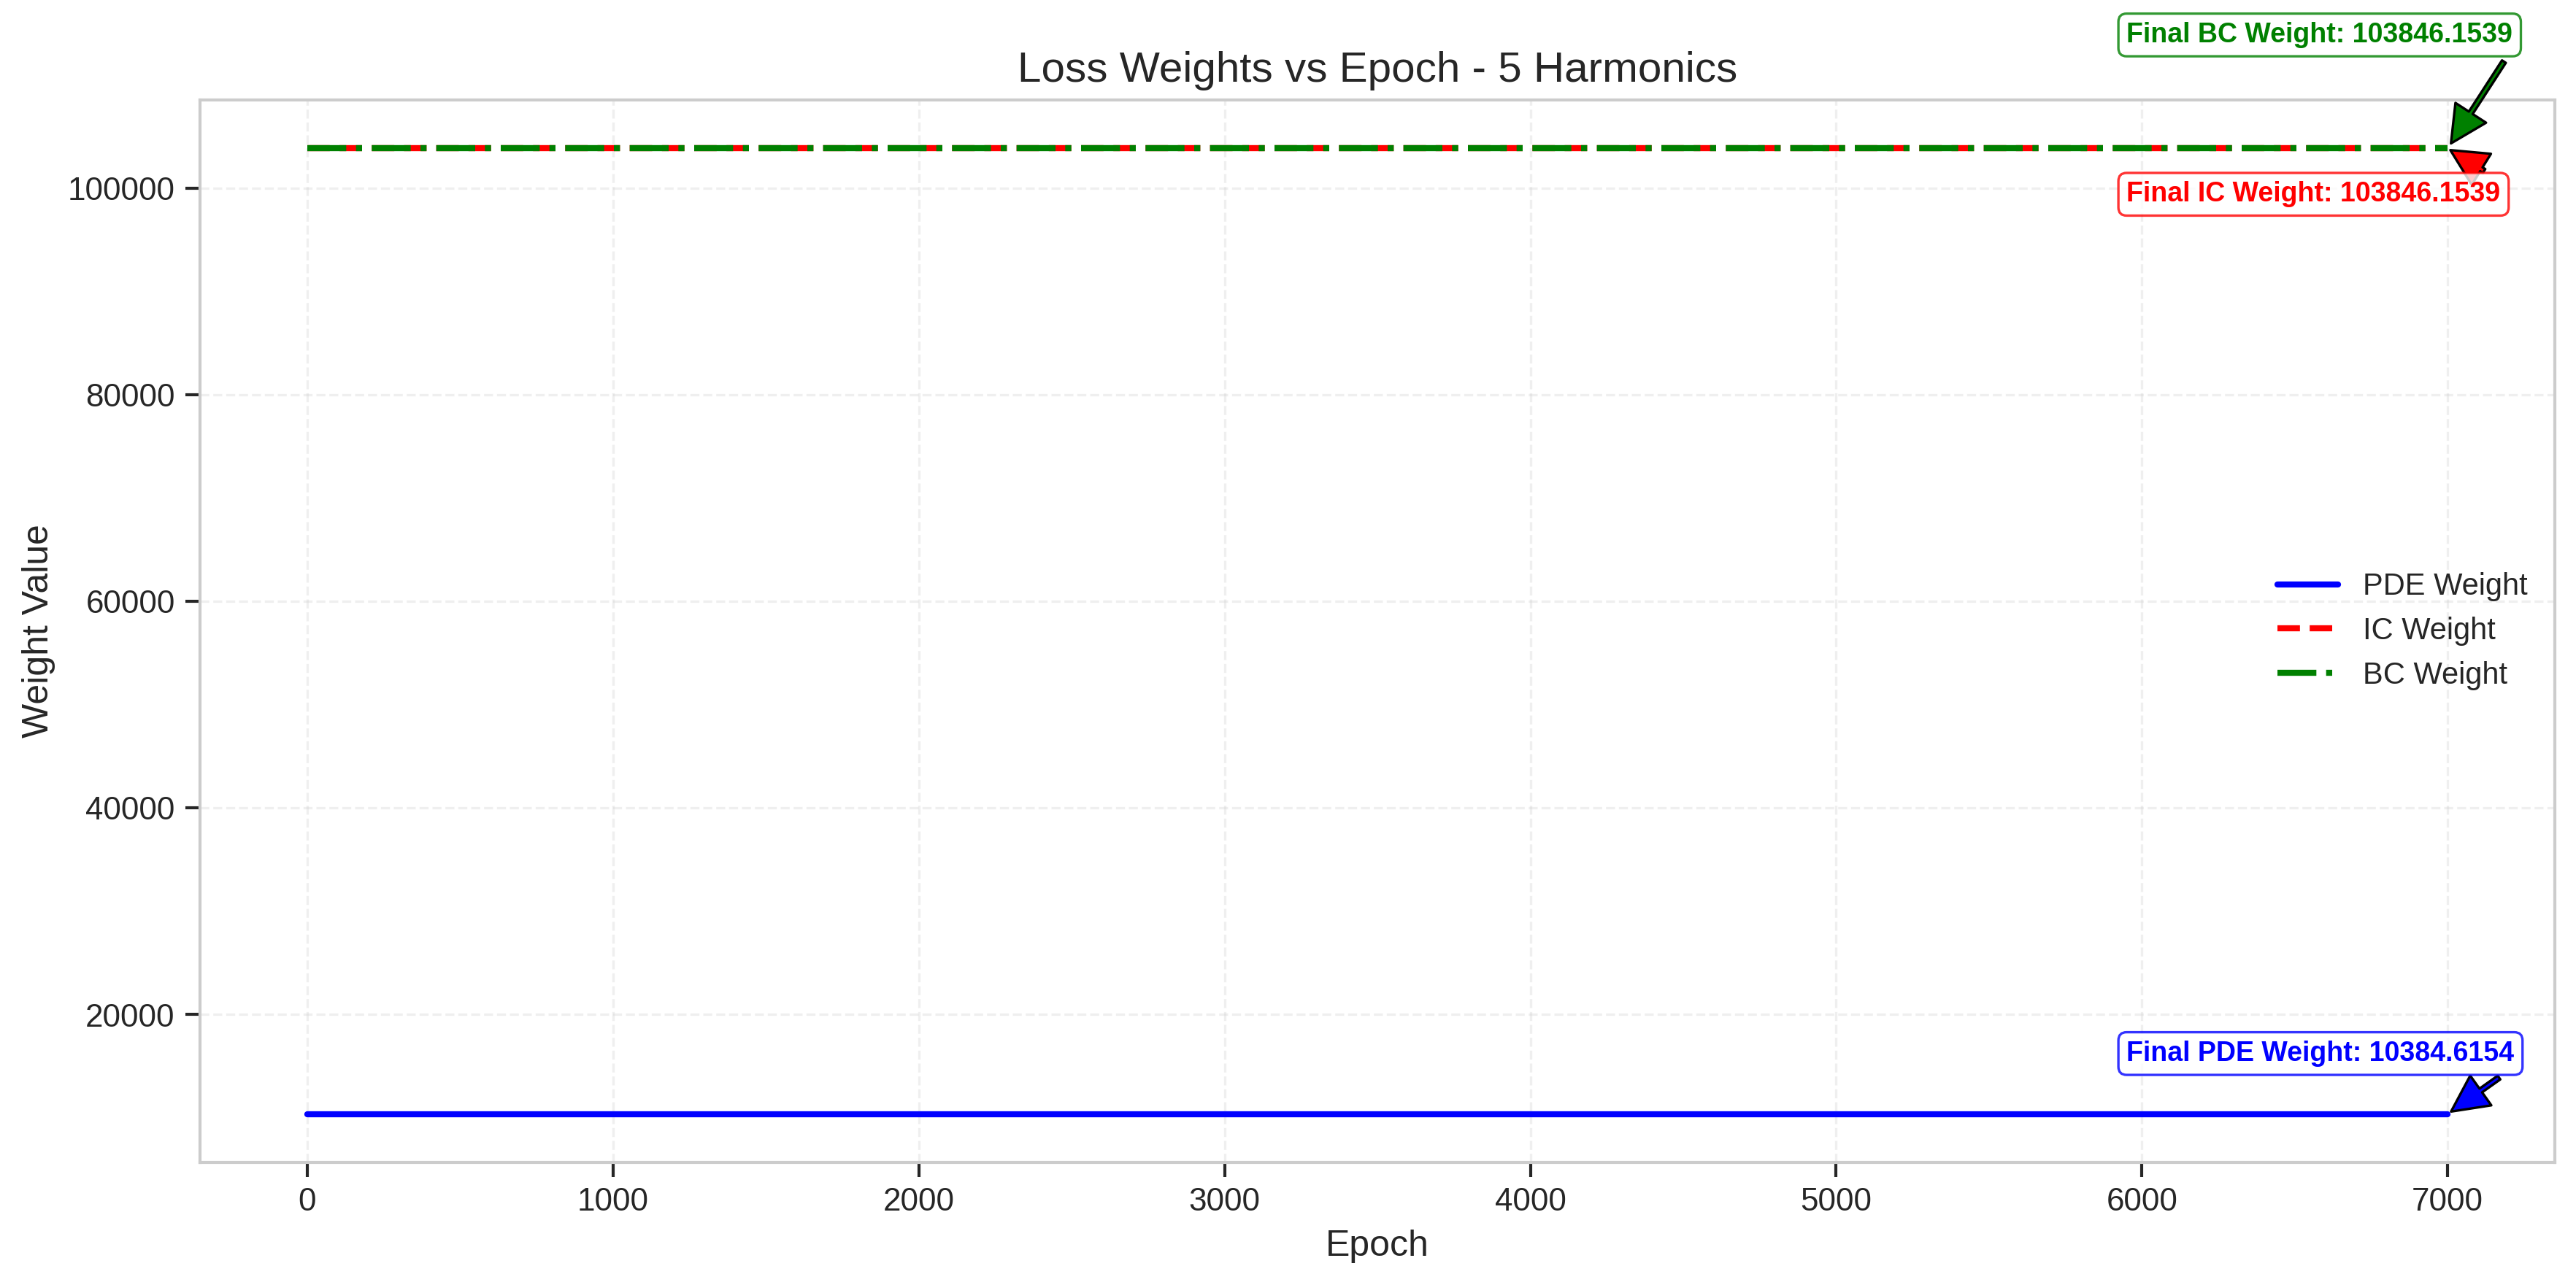
\includegraphics[width=\textwidth]{figures/weight_factors_5h.png}
        \caption{5 harmonics}
    \end{subfigure}
    \hfill
    \begin{subfigure}[b]{0.48\textwidth}
        \centering
        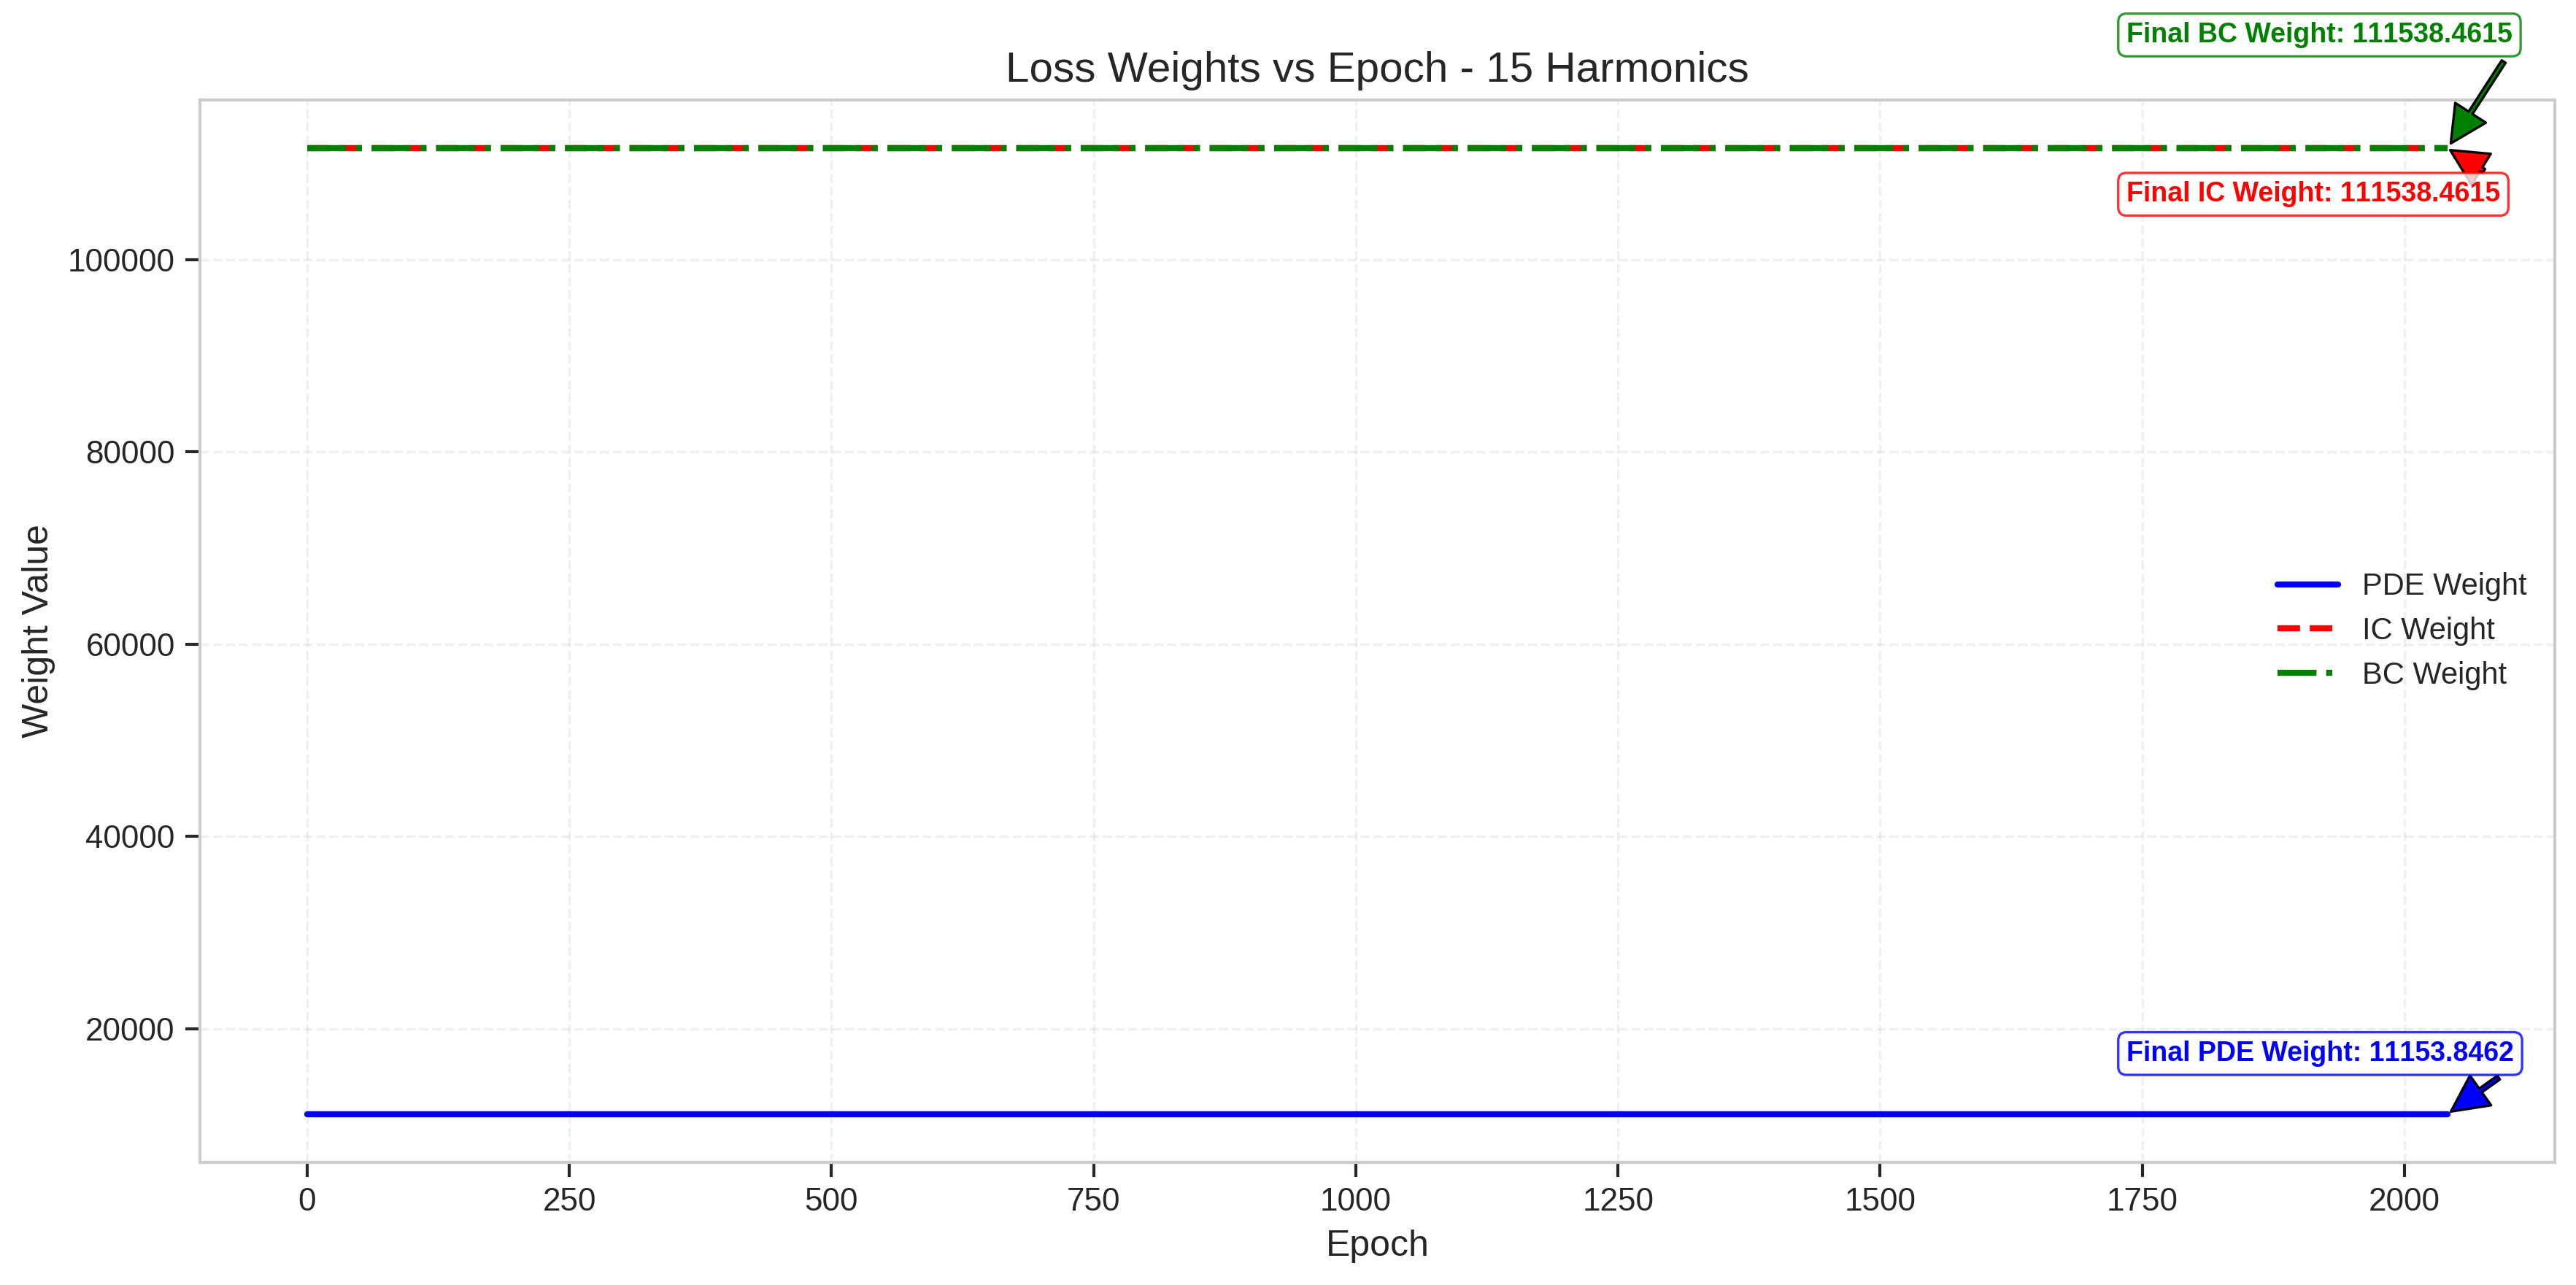
\includegraphics[width=\textwidth]{figures/weight_factors_15h.png}
        \caption{15 harmonics}
    \end{subfigure}
    \caption{Evolution of adaptive weight factors during training for different harmonic configurations, showing how the optimization balances competing loss components.}
    \label{fig:weight_comparison}
\end{figure}

\subsection{Solution Slice Comparisons}

\begin{figure}[H]
    \centering
    \begin{subfigure}[b]{0.48\textwidth}
        \centering
        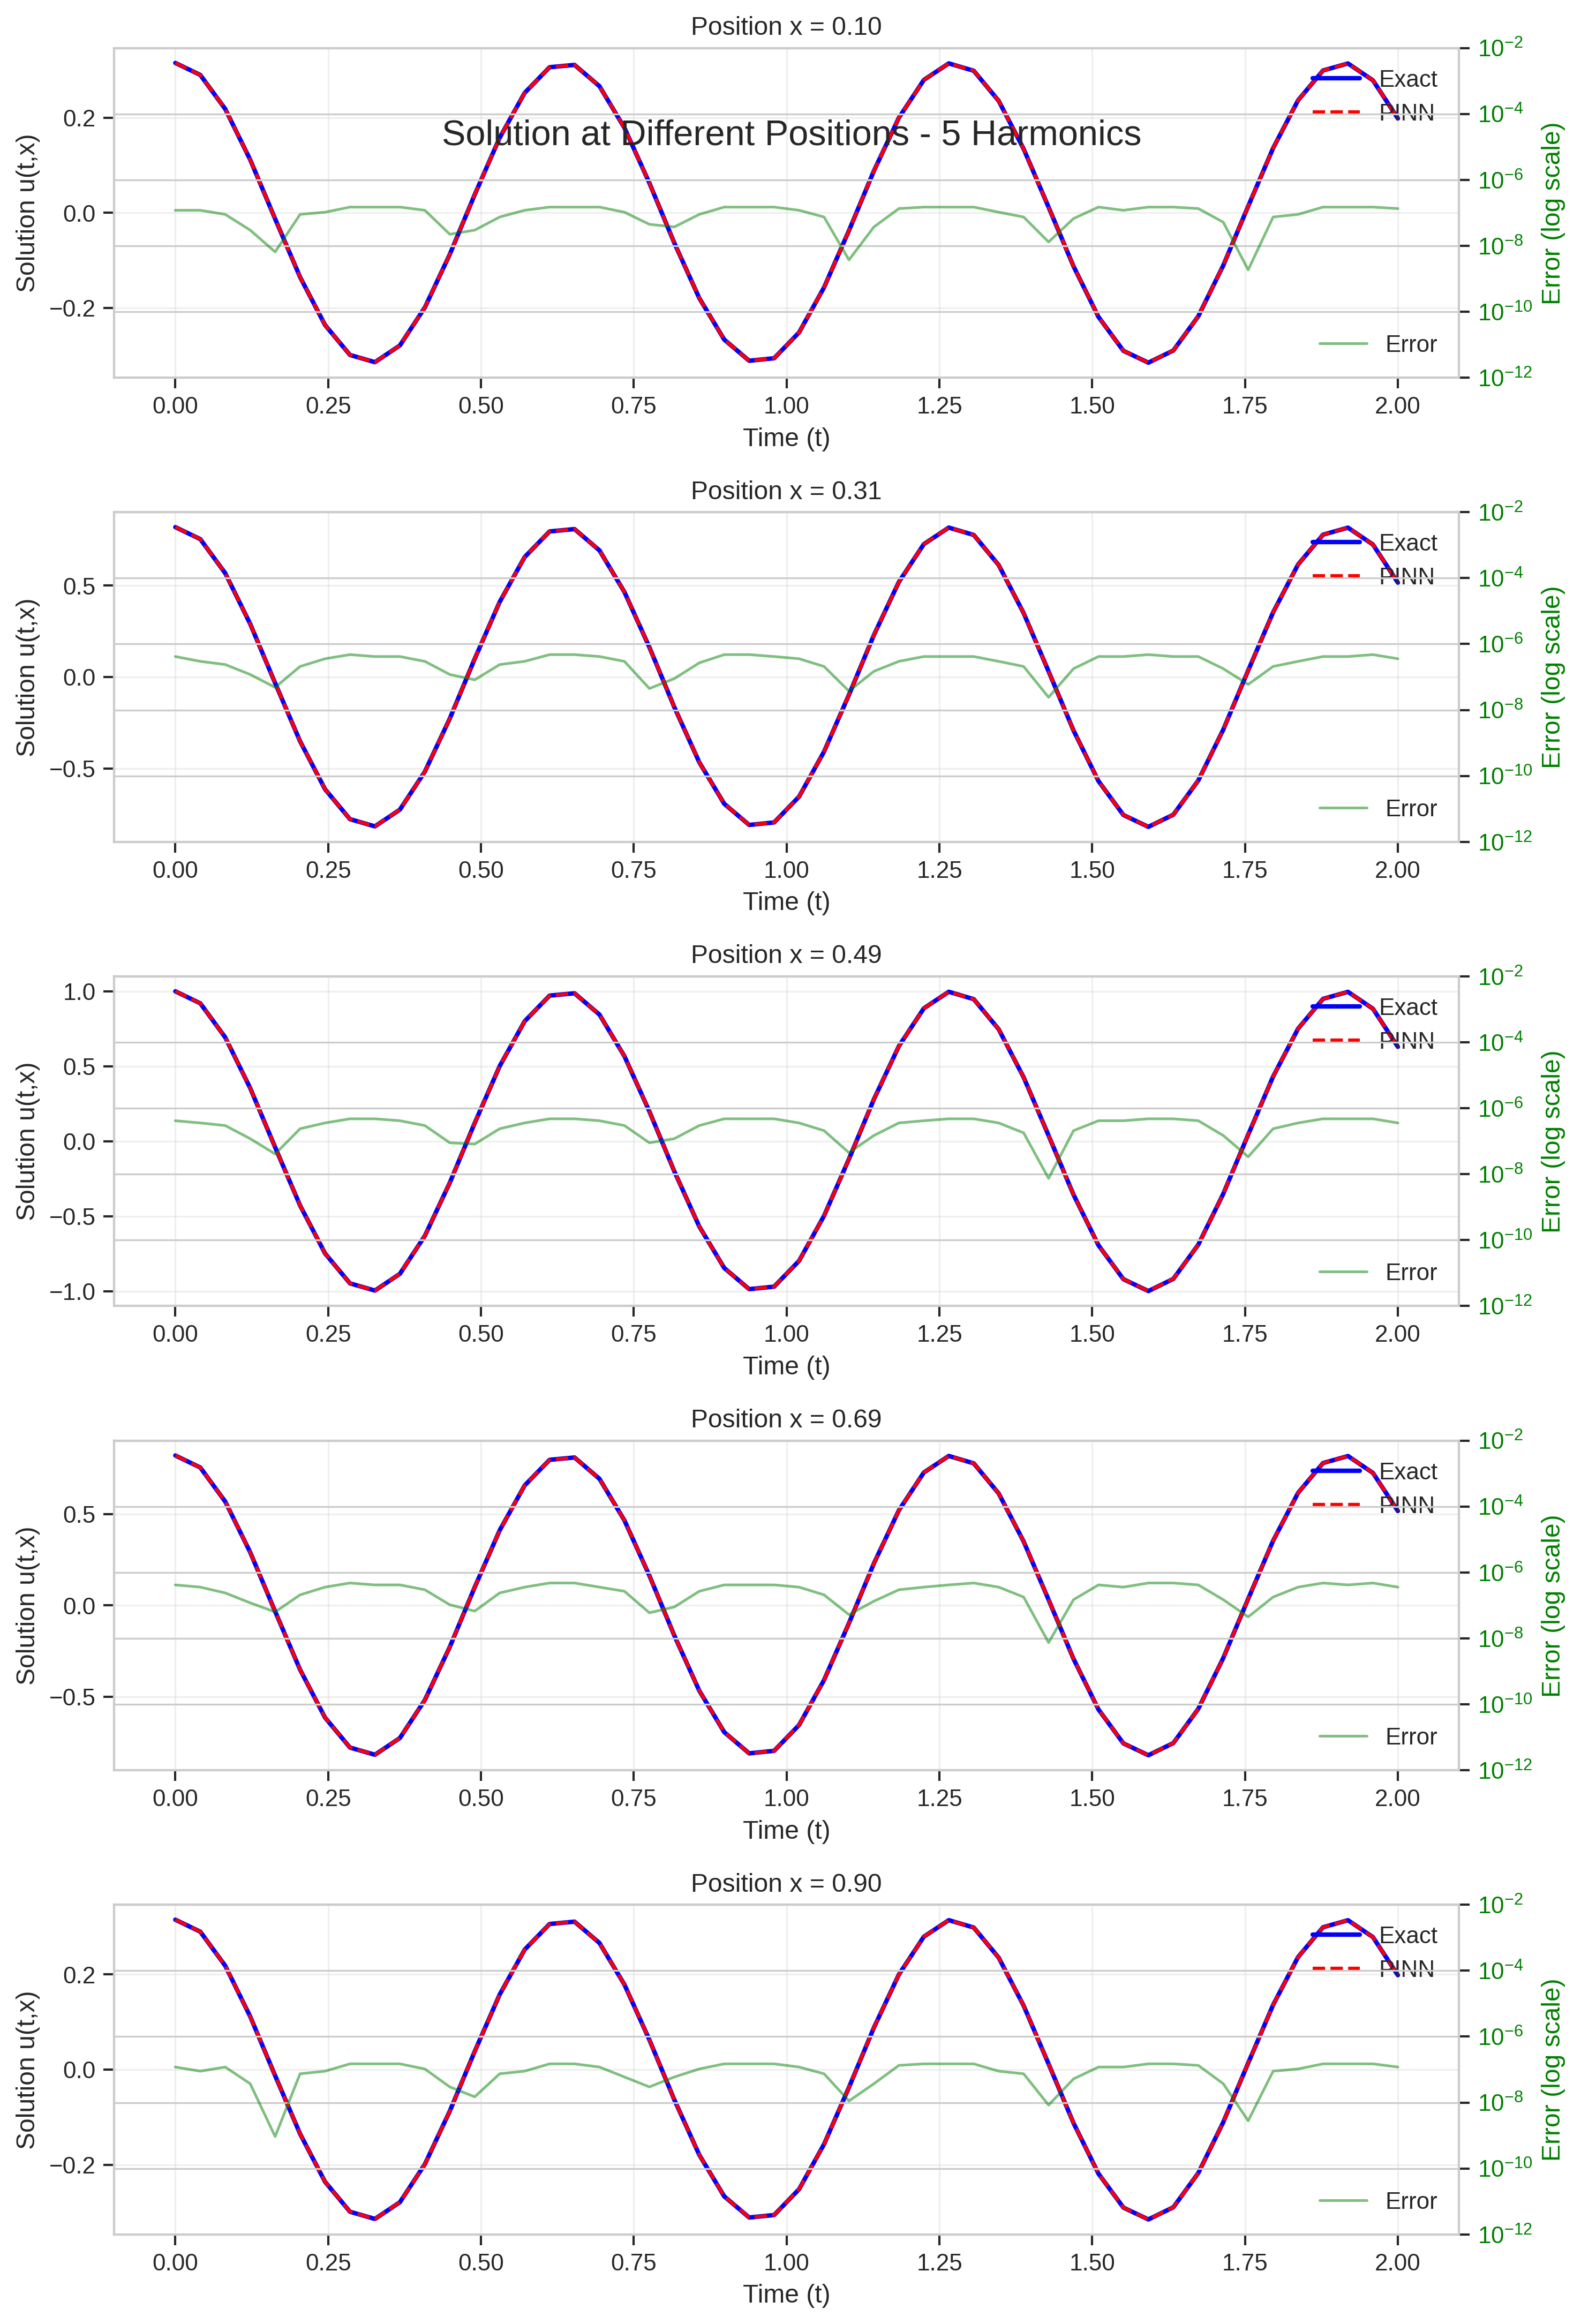
\includegraphics[width=\textwidth]{figures/space_slices_5h.png}
        \caption{Spatial slices - 5 harmonics}
    \end{subfigure}
    \hfill
    \begin{subfigure}[b]{0.48\textwidth}
        \centering
        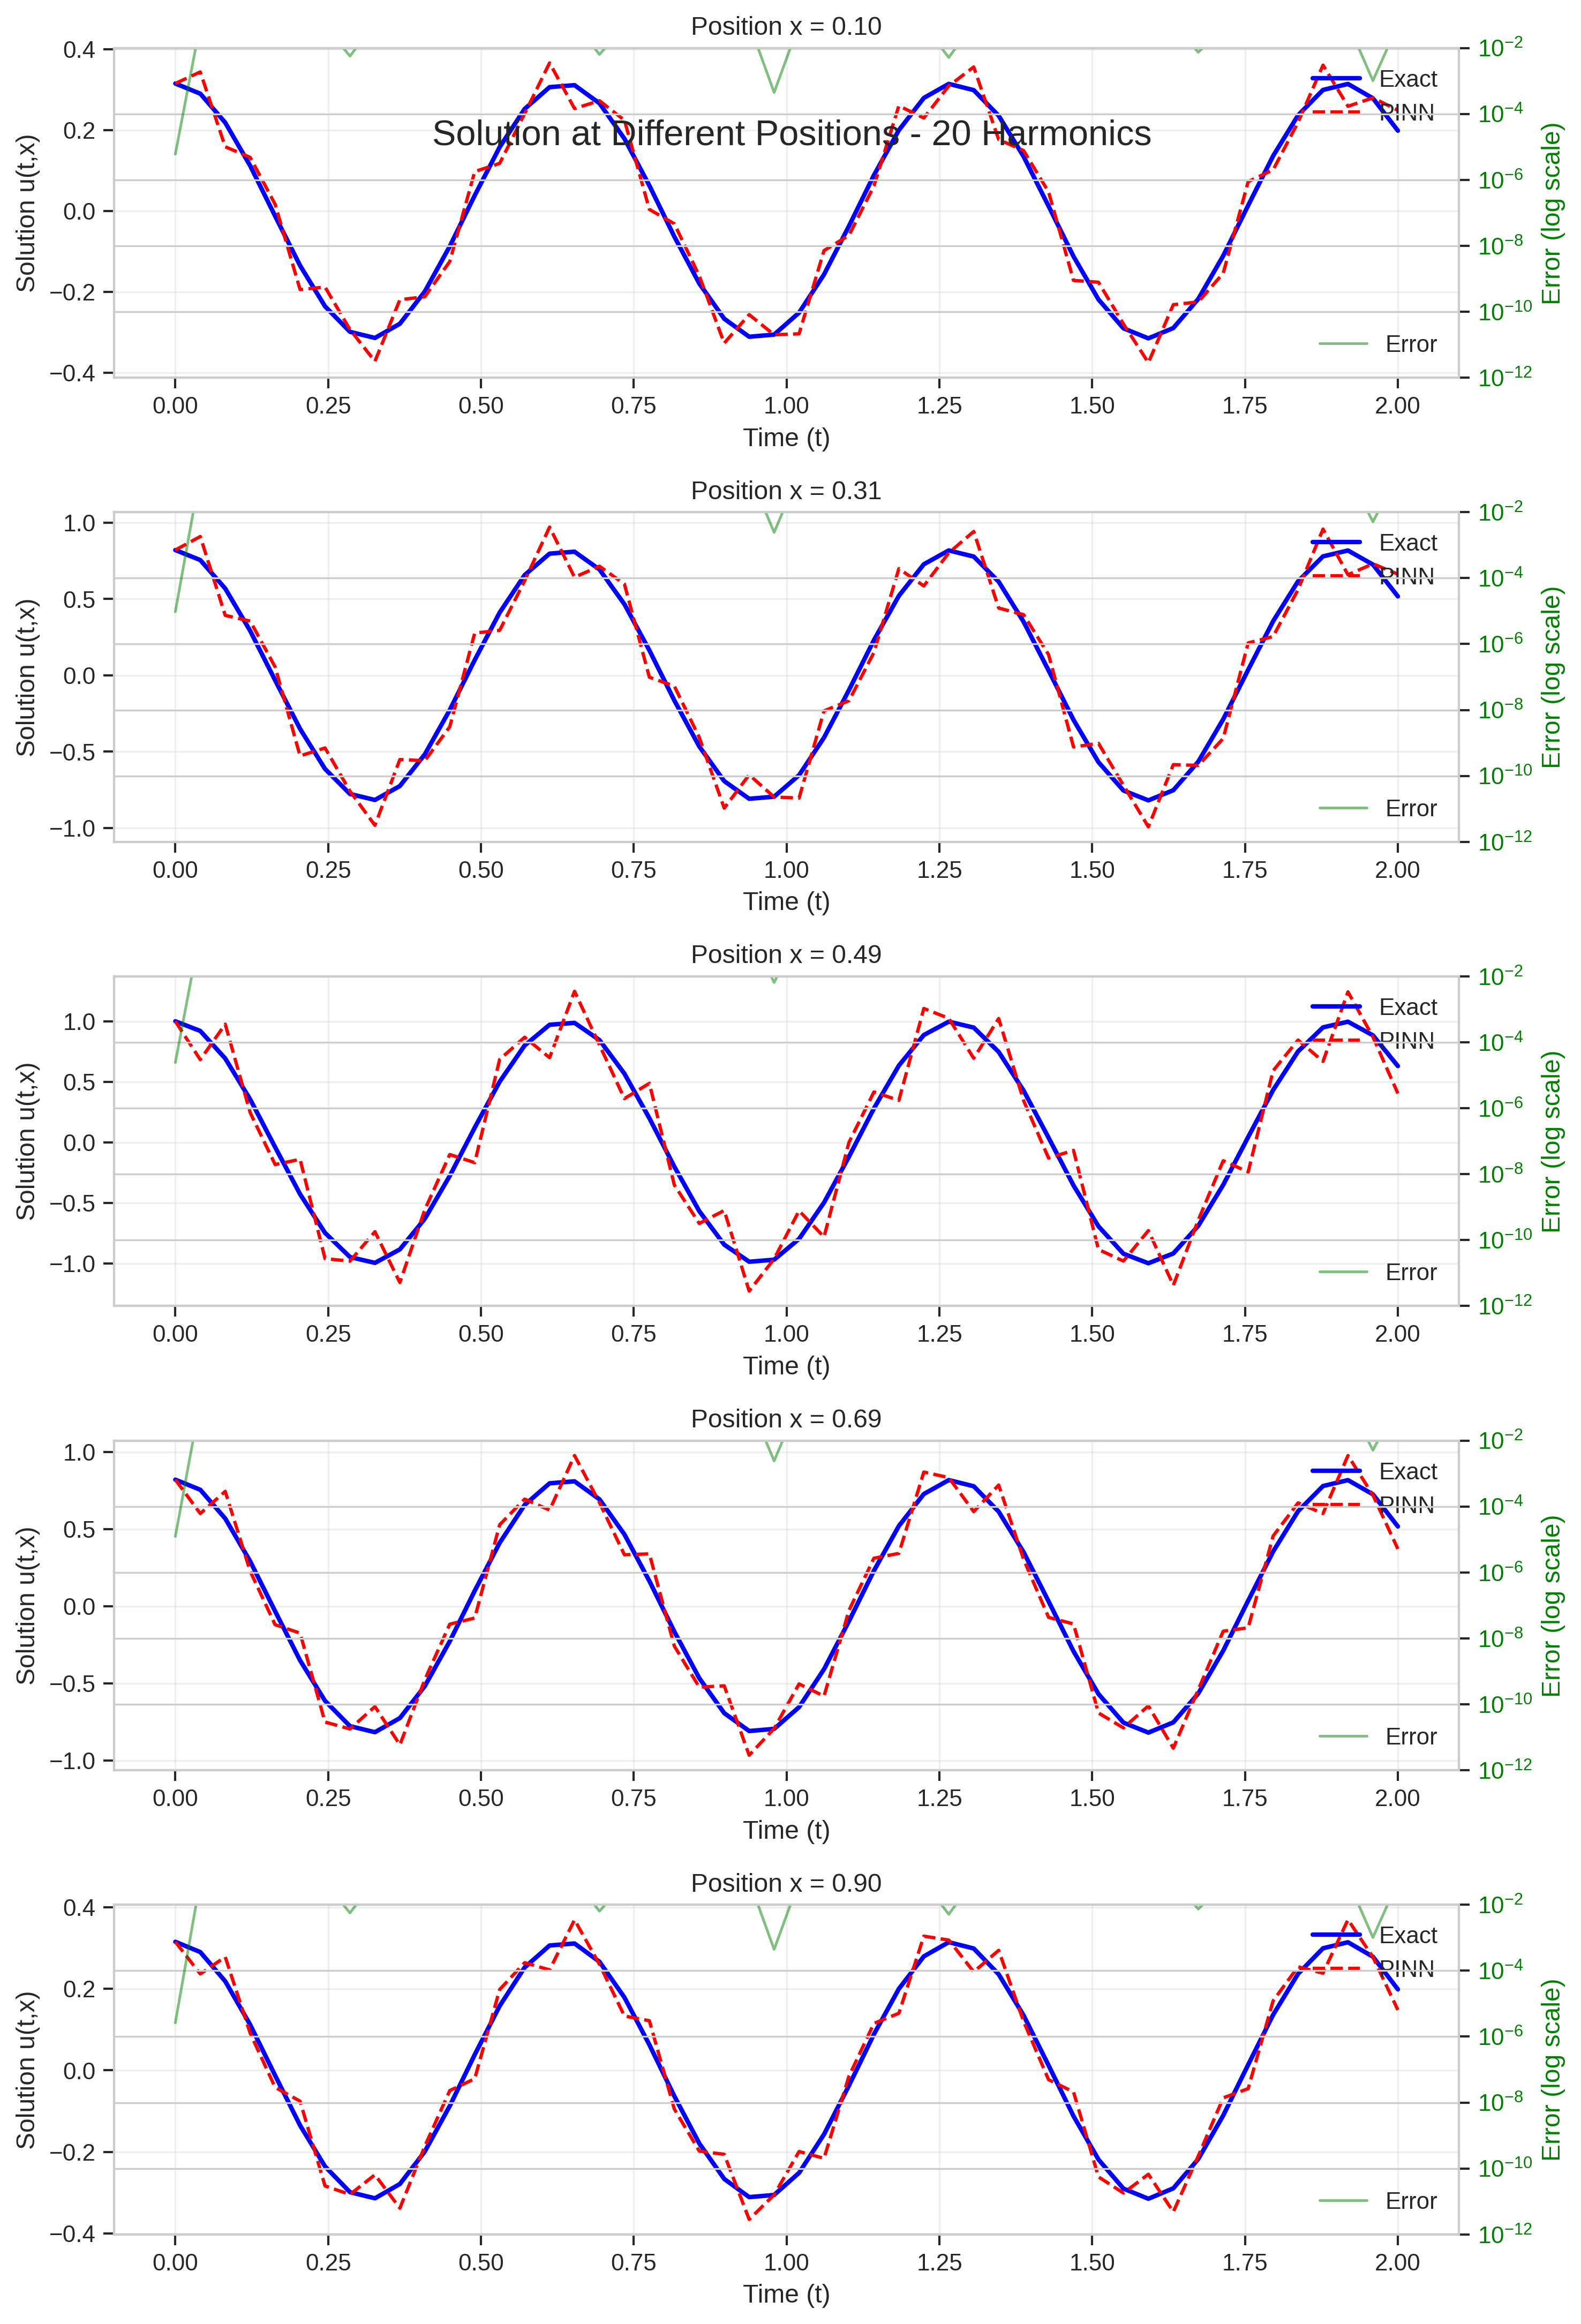
\includegraphics[width=\textwidth]{figures/space_slices_20h.png}
        \caption{Spatial slices - 20 harmonics}
    \end{subfigure}
    \caption{Spatial solution profiles at fixed time points, demonstrating accuracy variations across different harmonic configurations.}
    \label{fig:space_slice_comparison}
\end{figure}

\begin{figure}[H]
    \centering
    \begin{subfigure}[b]{0.48\textwidth}
        \centering
        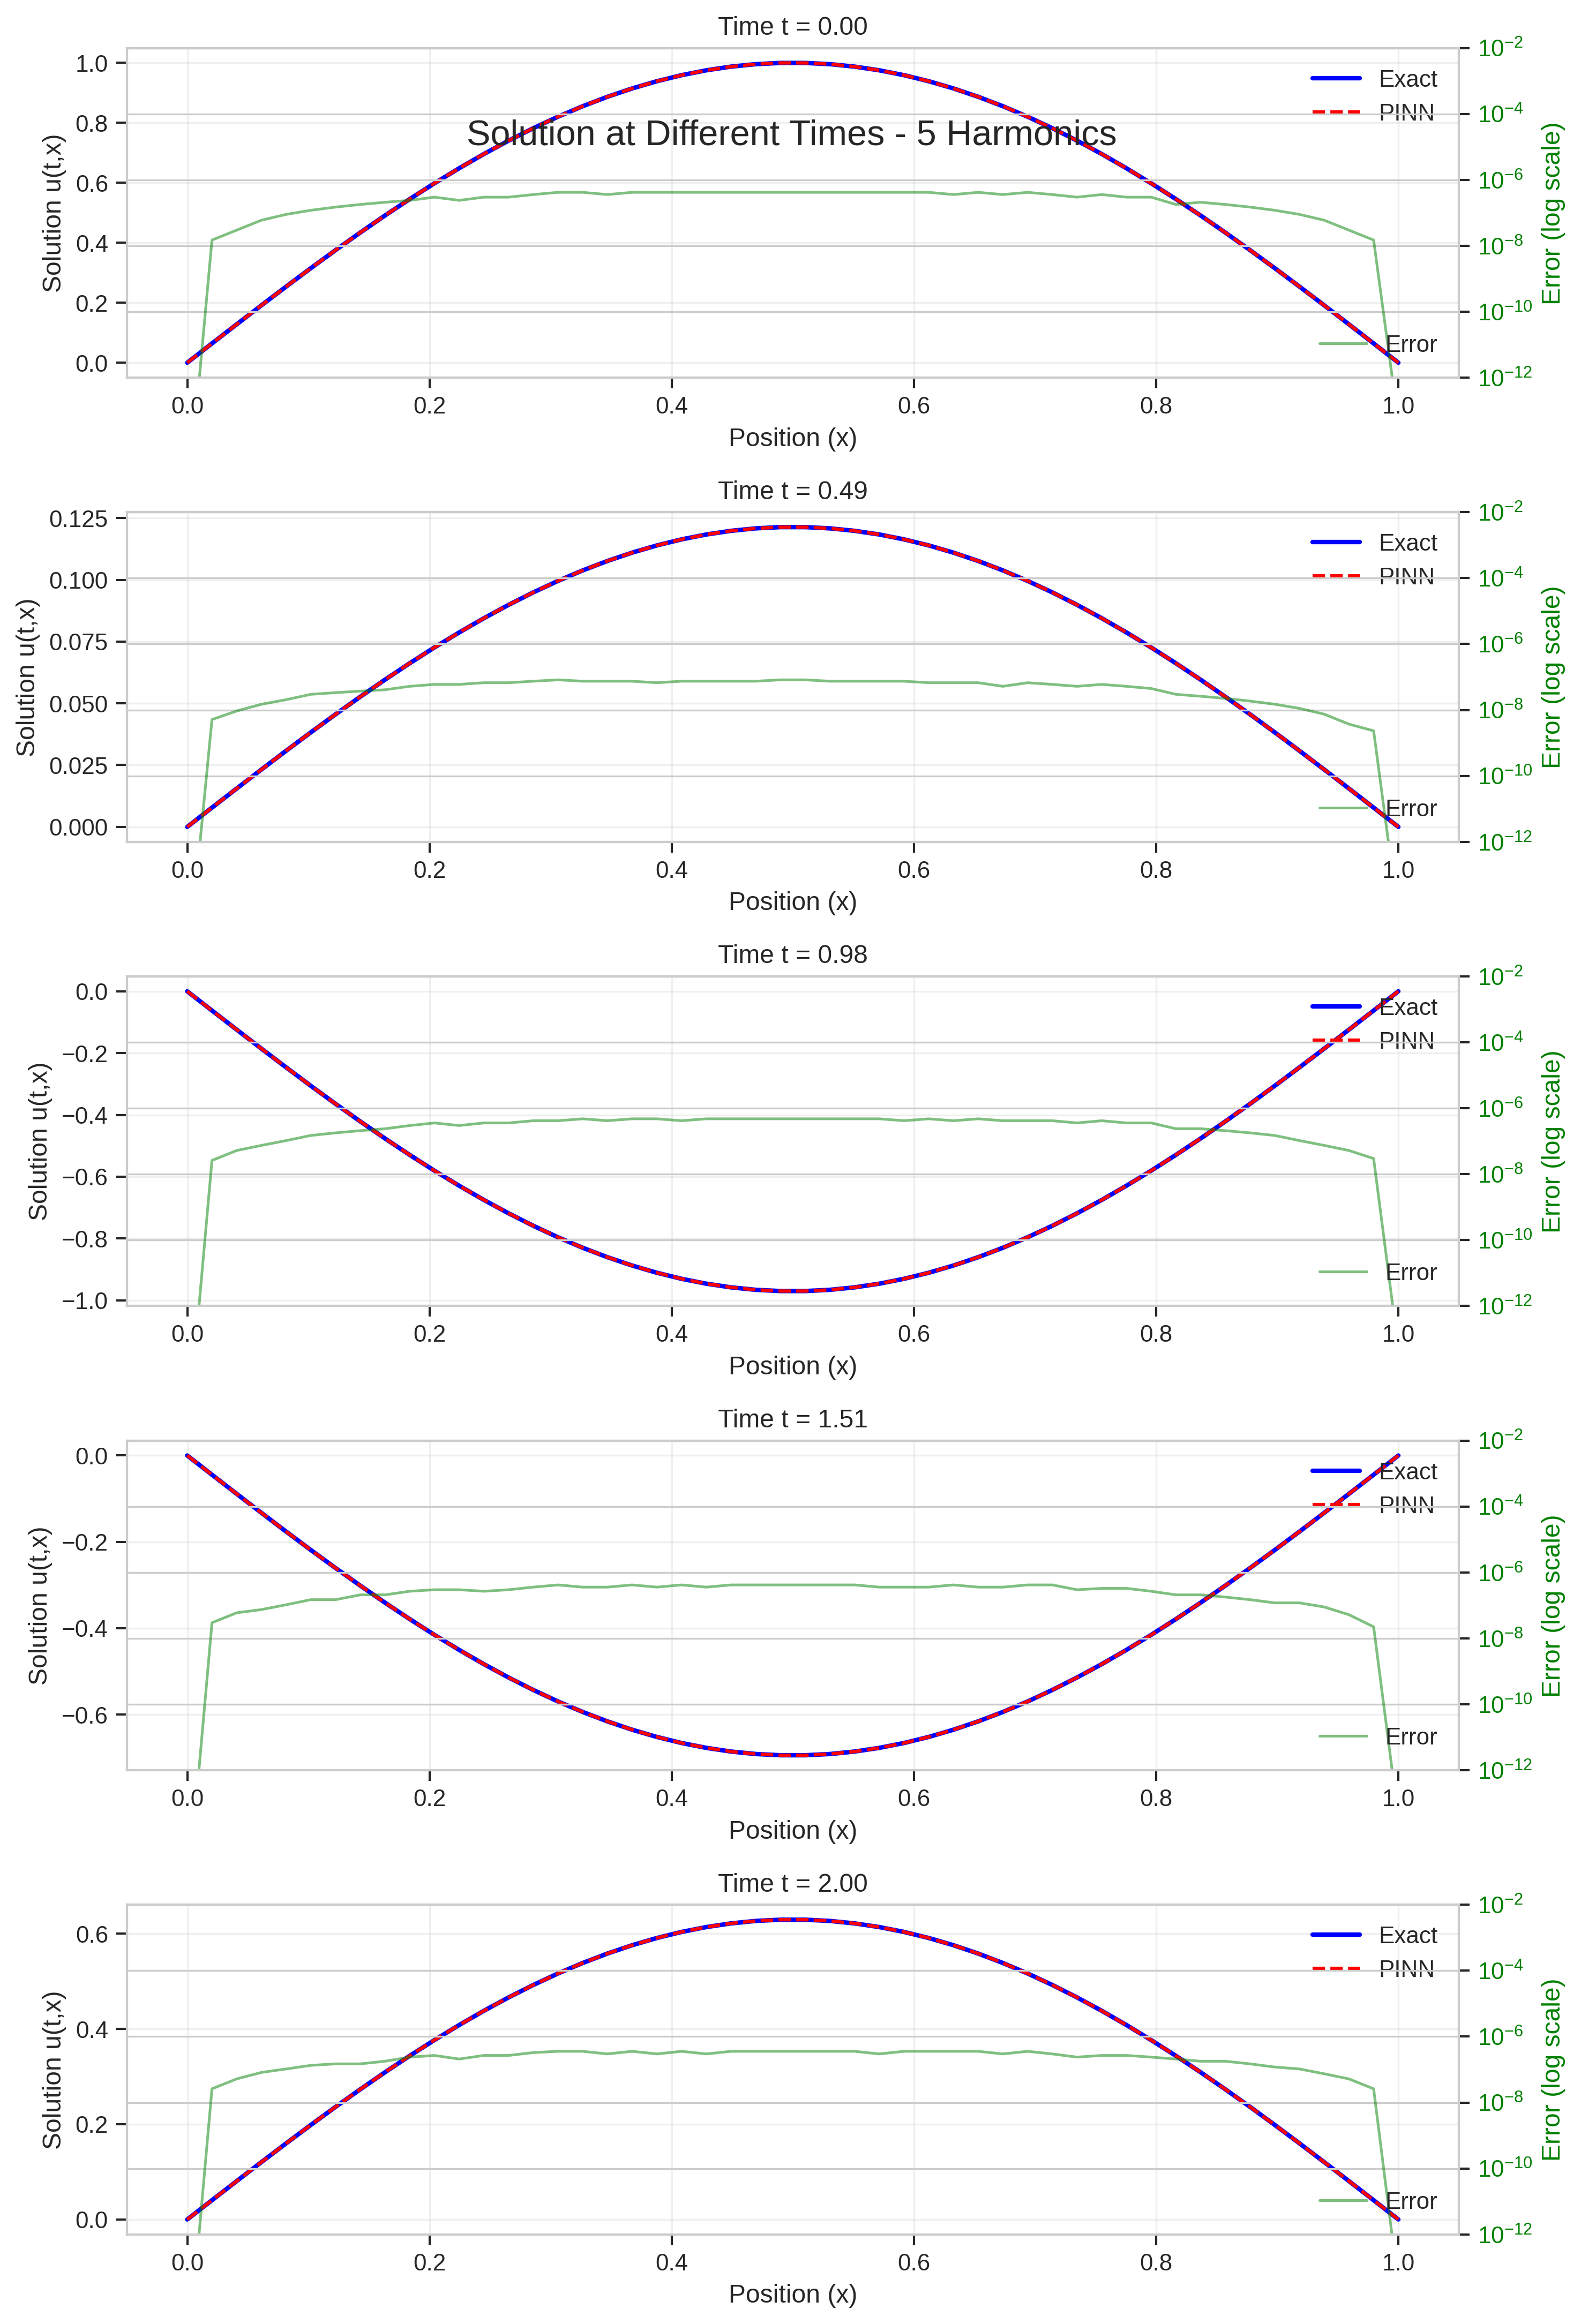
\includegraphics[width=\textwidth]{figures/time_slices_5h.png}
        \caption{Temporal slices - 5 harmonics}
    \end{subfigure}
    \hfill
    \begin{subfigure}[b]{0.48\textwidth}
        \centering
        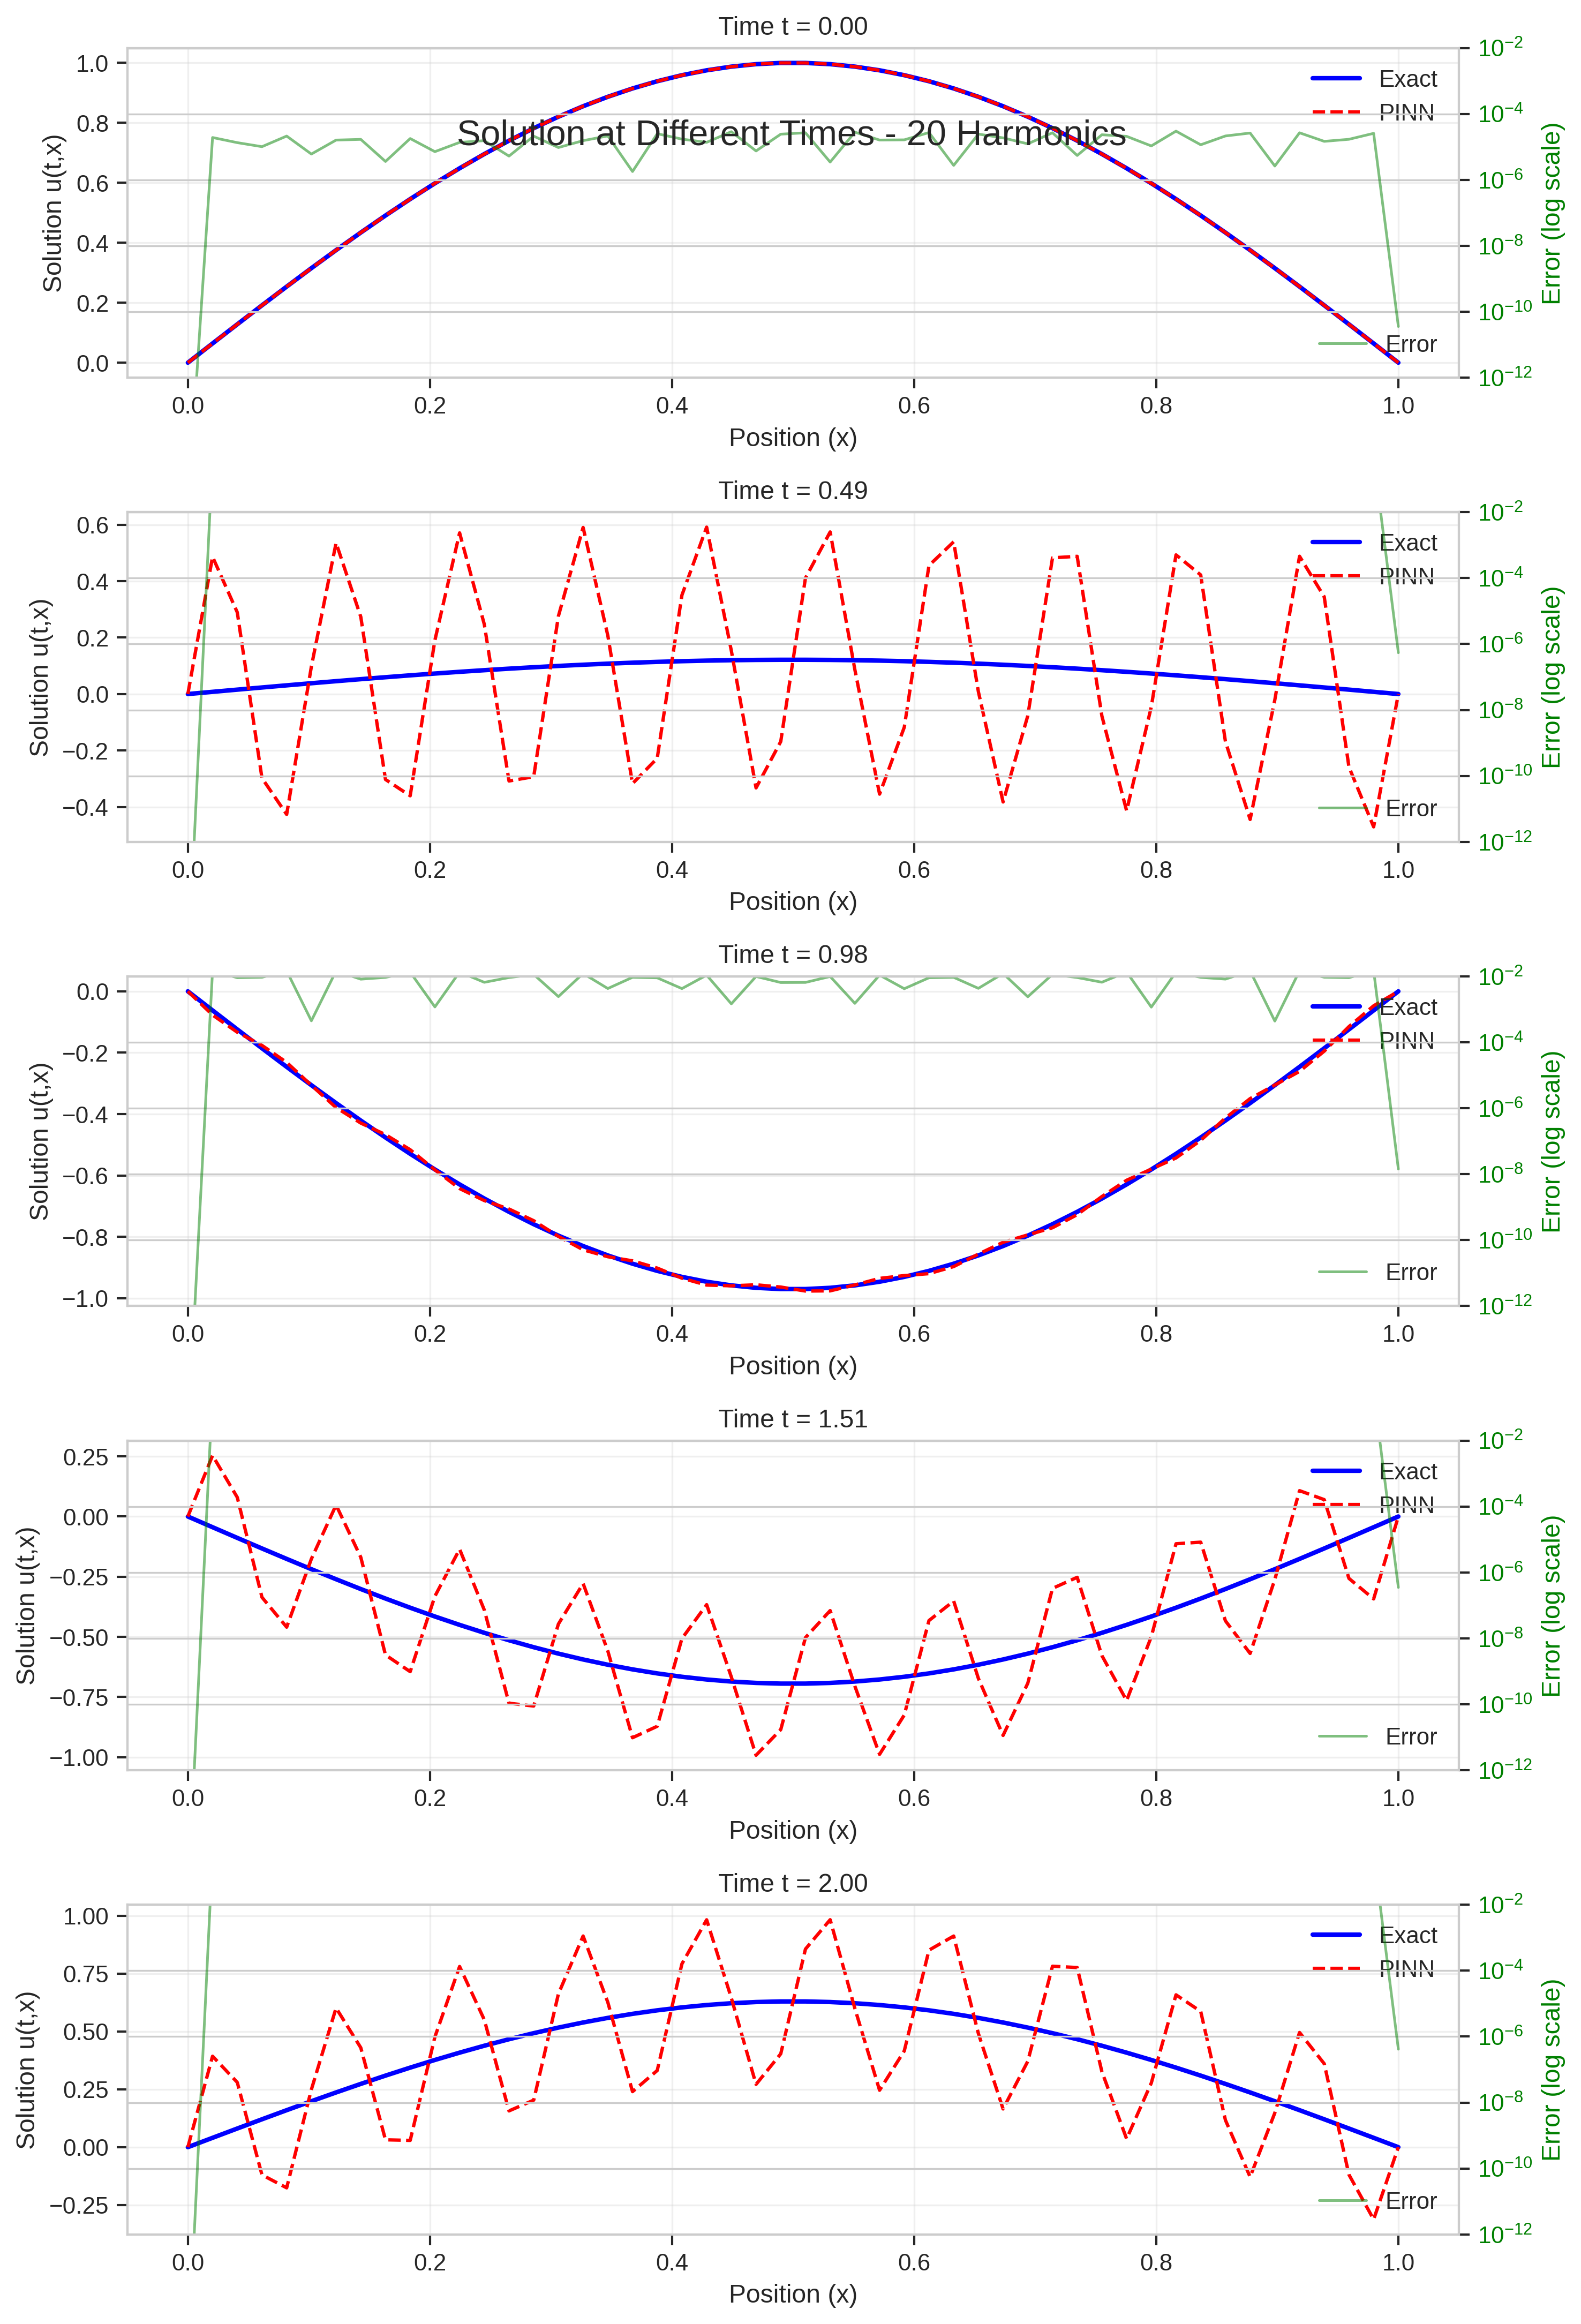
\includegraphics[width=\textwidth]{figures/time_slices_20h.png}
        \caption{Temporal slices - 20 harmonics}
    \end{subfigure}
    \caption{Temporal evolution at fixed spatial locations, showing how different harmonic counts affect time-dependent accuracy.}
    \label{fig:time_slice_comparison}
\end{figure}

\subsection{Comprehensive Error Comparison}

\begin{figure}[H]
    \centering
    \begin{subfigure}[b]{0.48\textwidth}
        \centering
        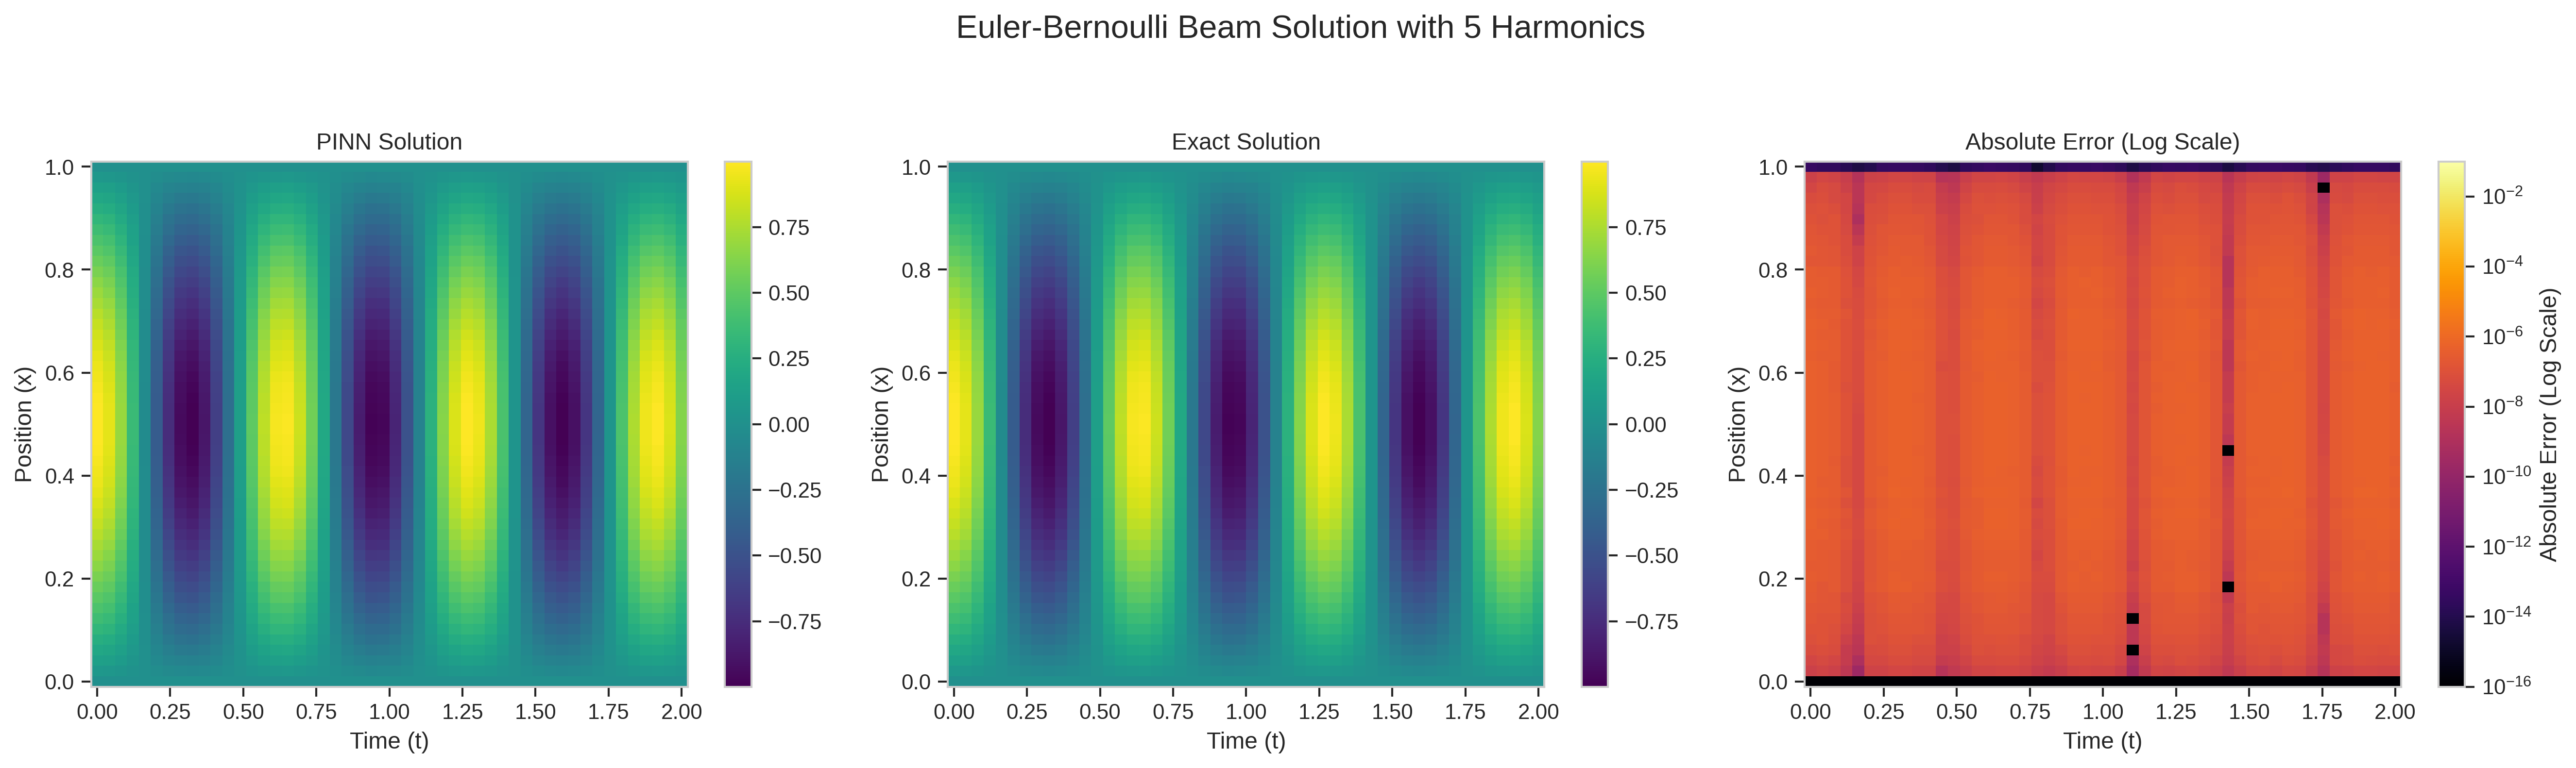
\includegraphics[width=\textwidth]{figures/comparison_5h.png}
        \caption{5 harmonics comparison}
    \end{subfigure}
    \hfill
    \begin{subfigure}[b]{0.48\textwidth}
        \centering
        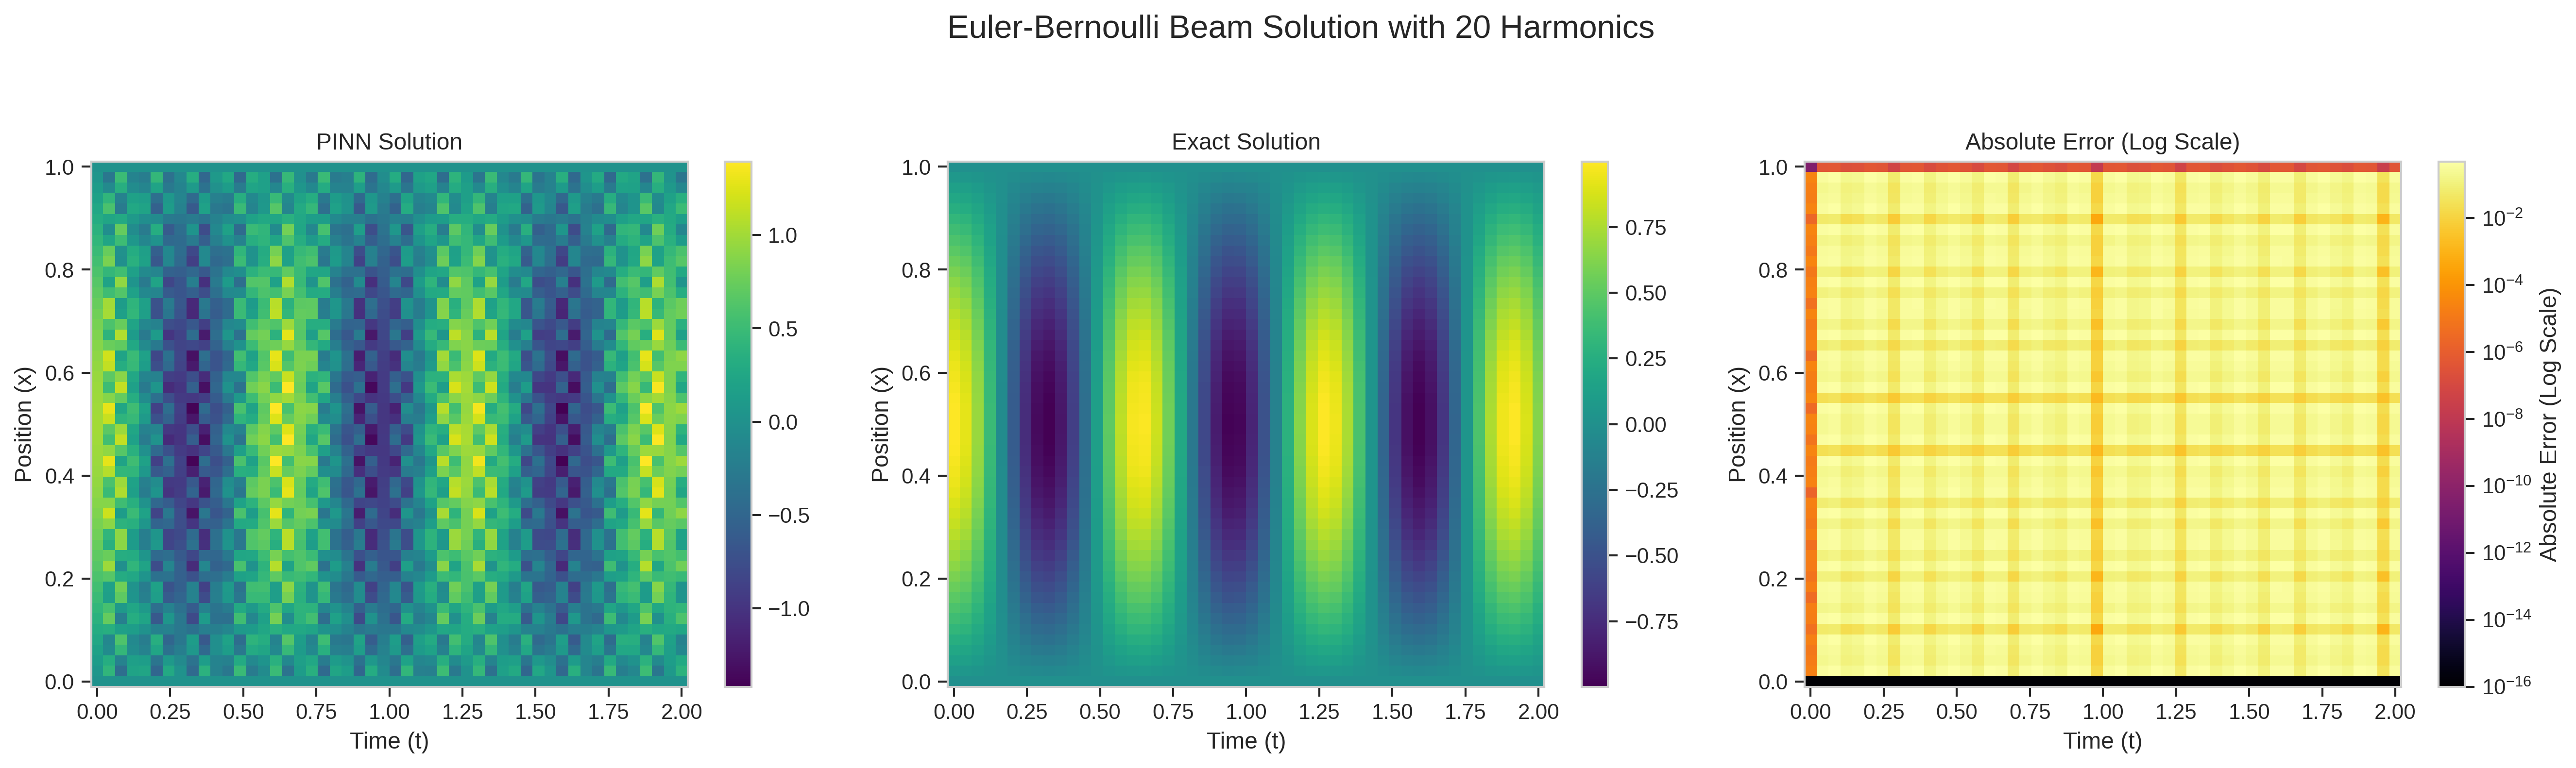
\includegraphics[width=\textwidth]{figures/comparison_20h.png}
        \caption{20 harmonics comparison}
    \end{subfigure}
    \caption{Direct comparison between PINN predictions, exact solutions, and absolute errors for representative harmonic configurations.}
    \label{fig:direct_comparison}
\end{figure}

The comprehensive results presented in this appendix confirm the optimal performance at 10 harmonics. The degradation observed for higher harmonic counts stems from: (1) increased parameter space dimensionality leading to more complex optimization landscapes, (2) overfitting to training data despite physics-informed regularization, and (3) numerical instabilities in computing high-order derivatives for numerous frequency components. These findings underscore the importance of architectural design choices in achieving ultra-precision solutions for physics-informed neural networks.

\section{Complete Experimental Results}

This section presents all additional experimental results not shown in the main text, providing a comprehensive view of the model's performance across all tested configurations.

\subsection{3D Error Visualizations}

\begin{figure}[H]
    \centering
    \begin{subfigure}[b]{0.32\textwidth}
        \centering
        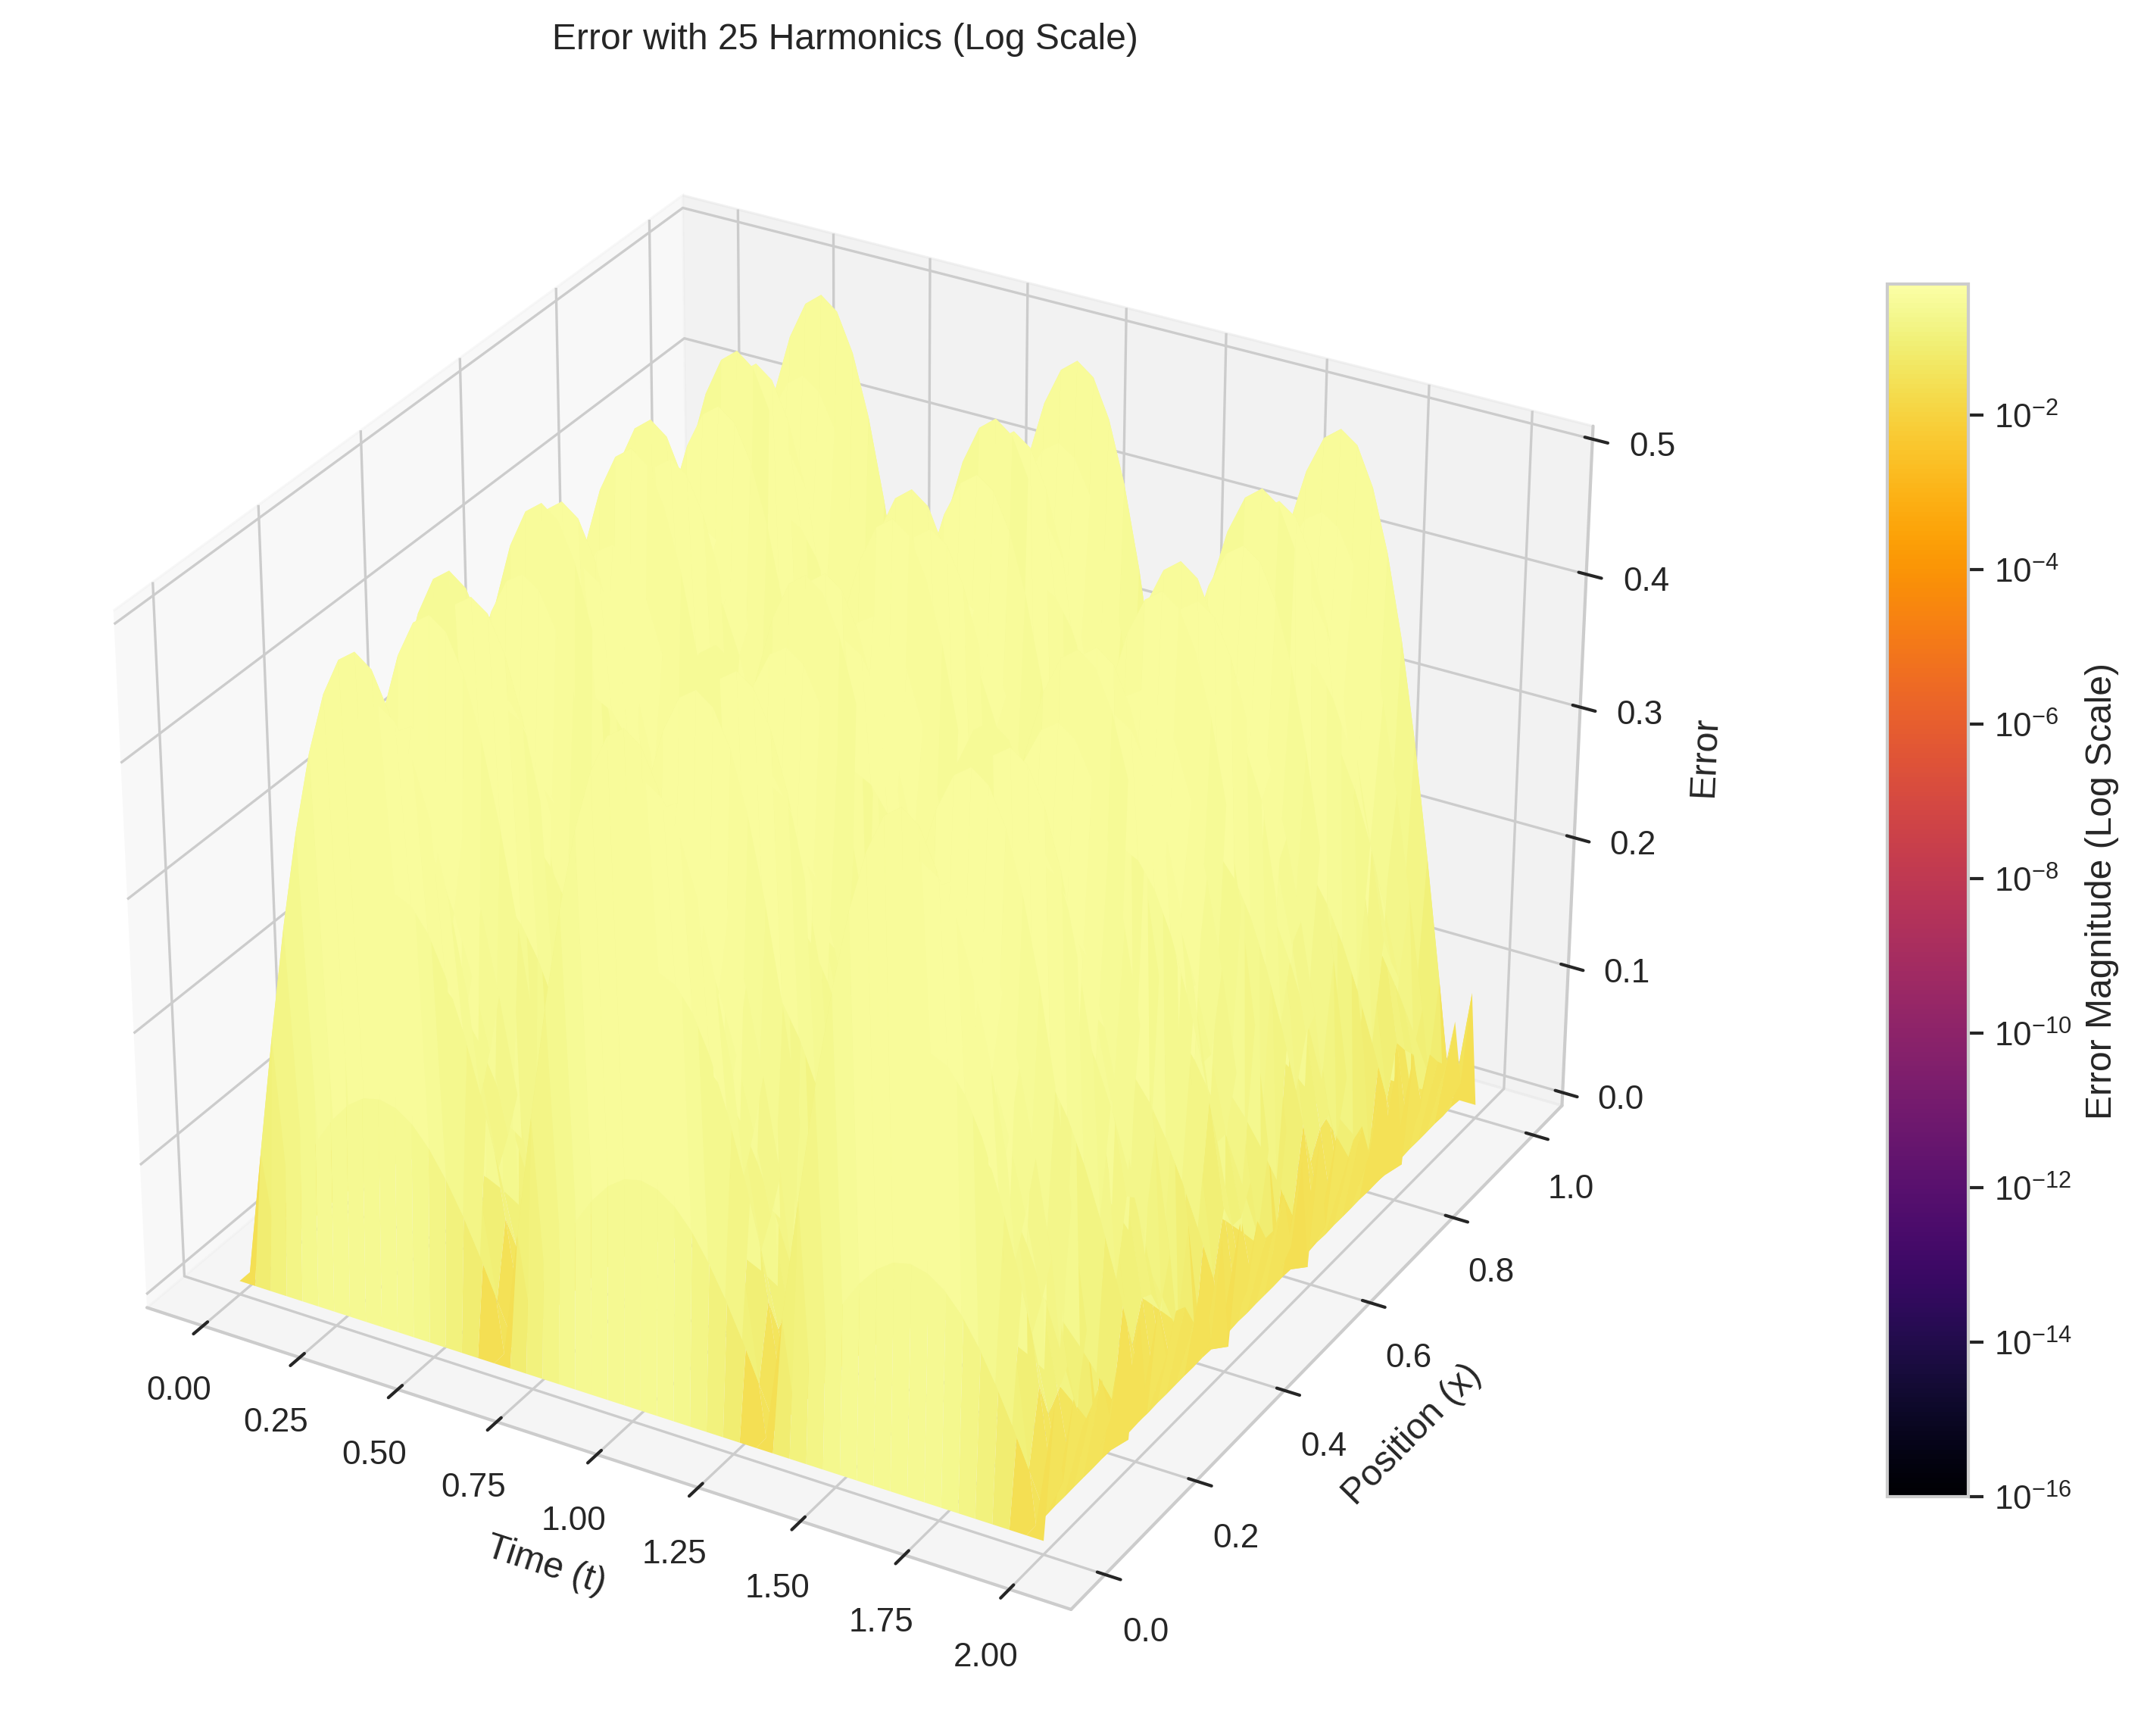
\includegraphics[width=\textwidth]{figures/3d_comparison_error_25h.png}
        \caption{25 harmonics}
    \end{subfigure}
    \hfill
    \begin{subfigure}[b]{0.32\textwidth}
        \centering
        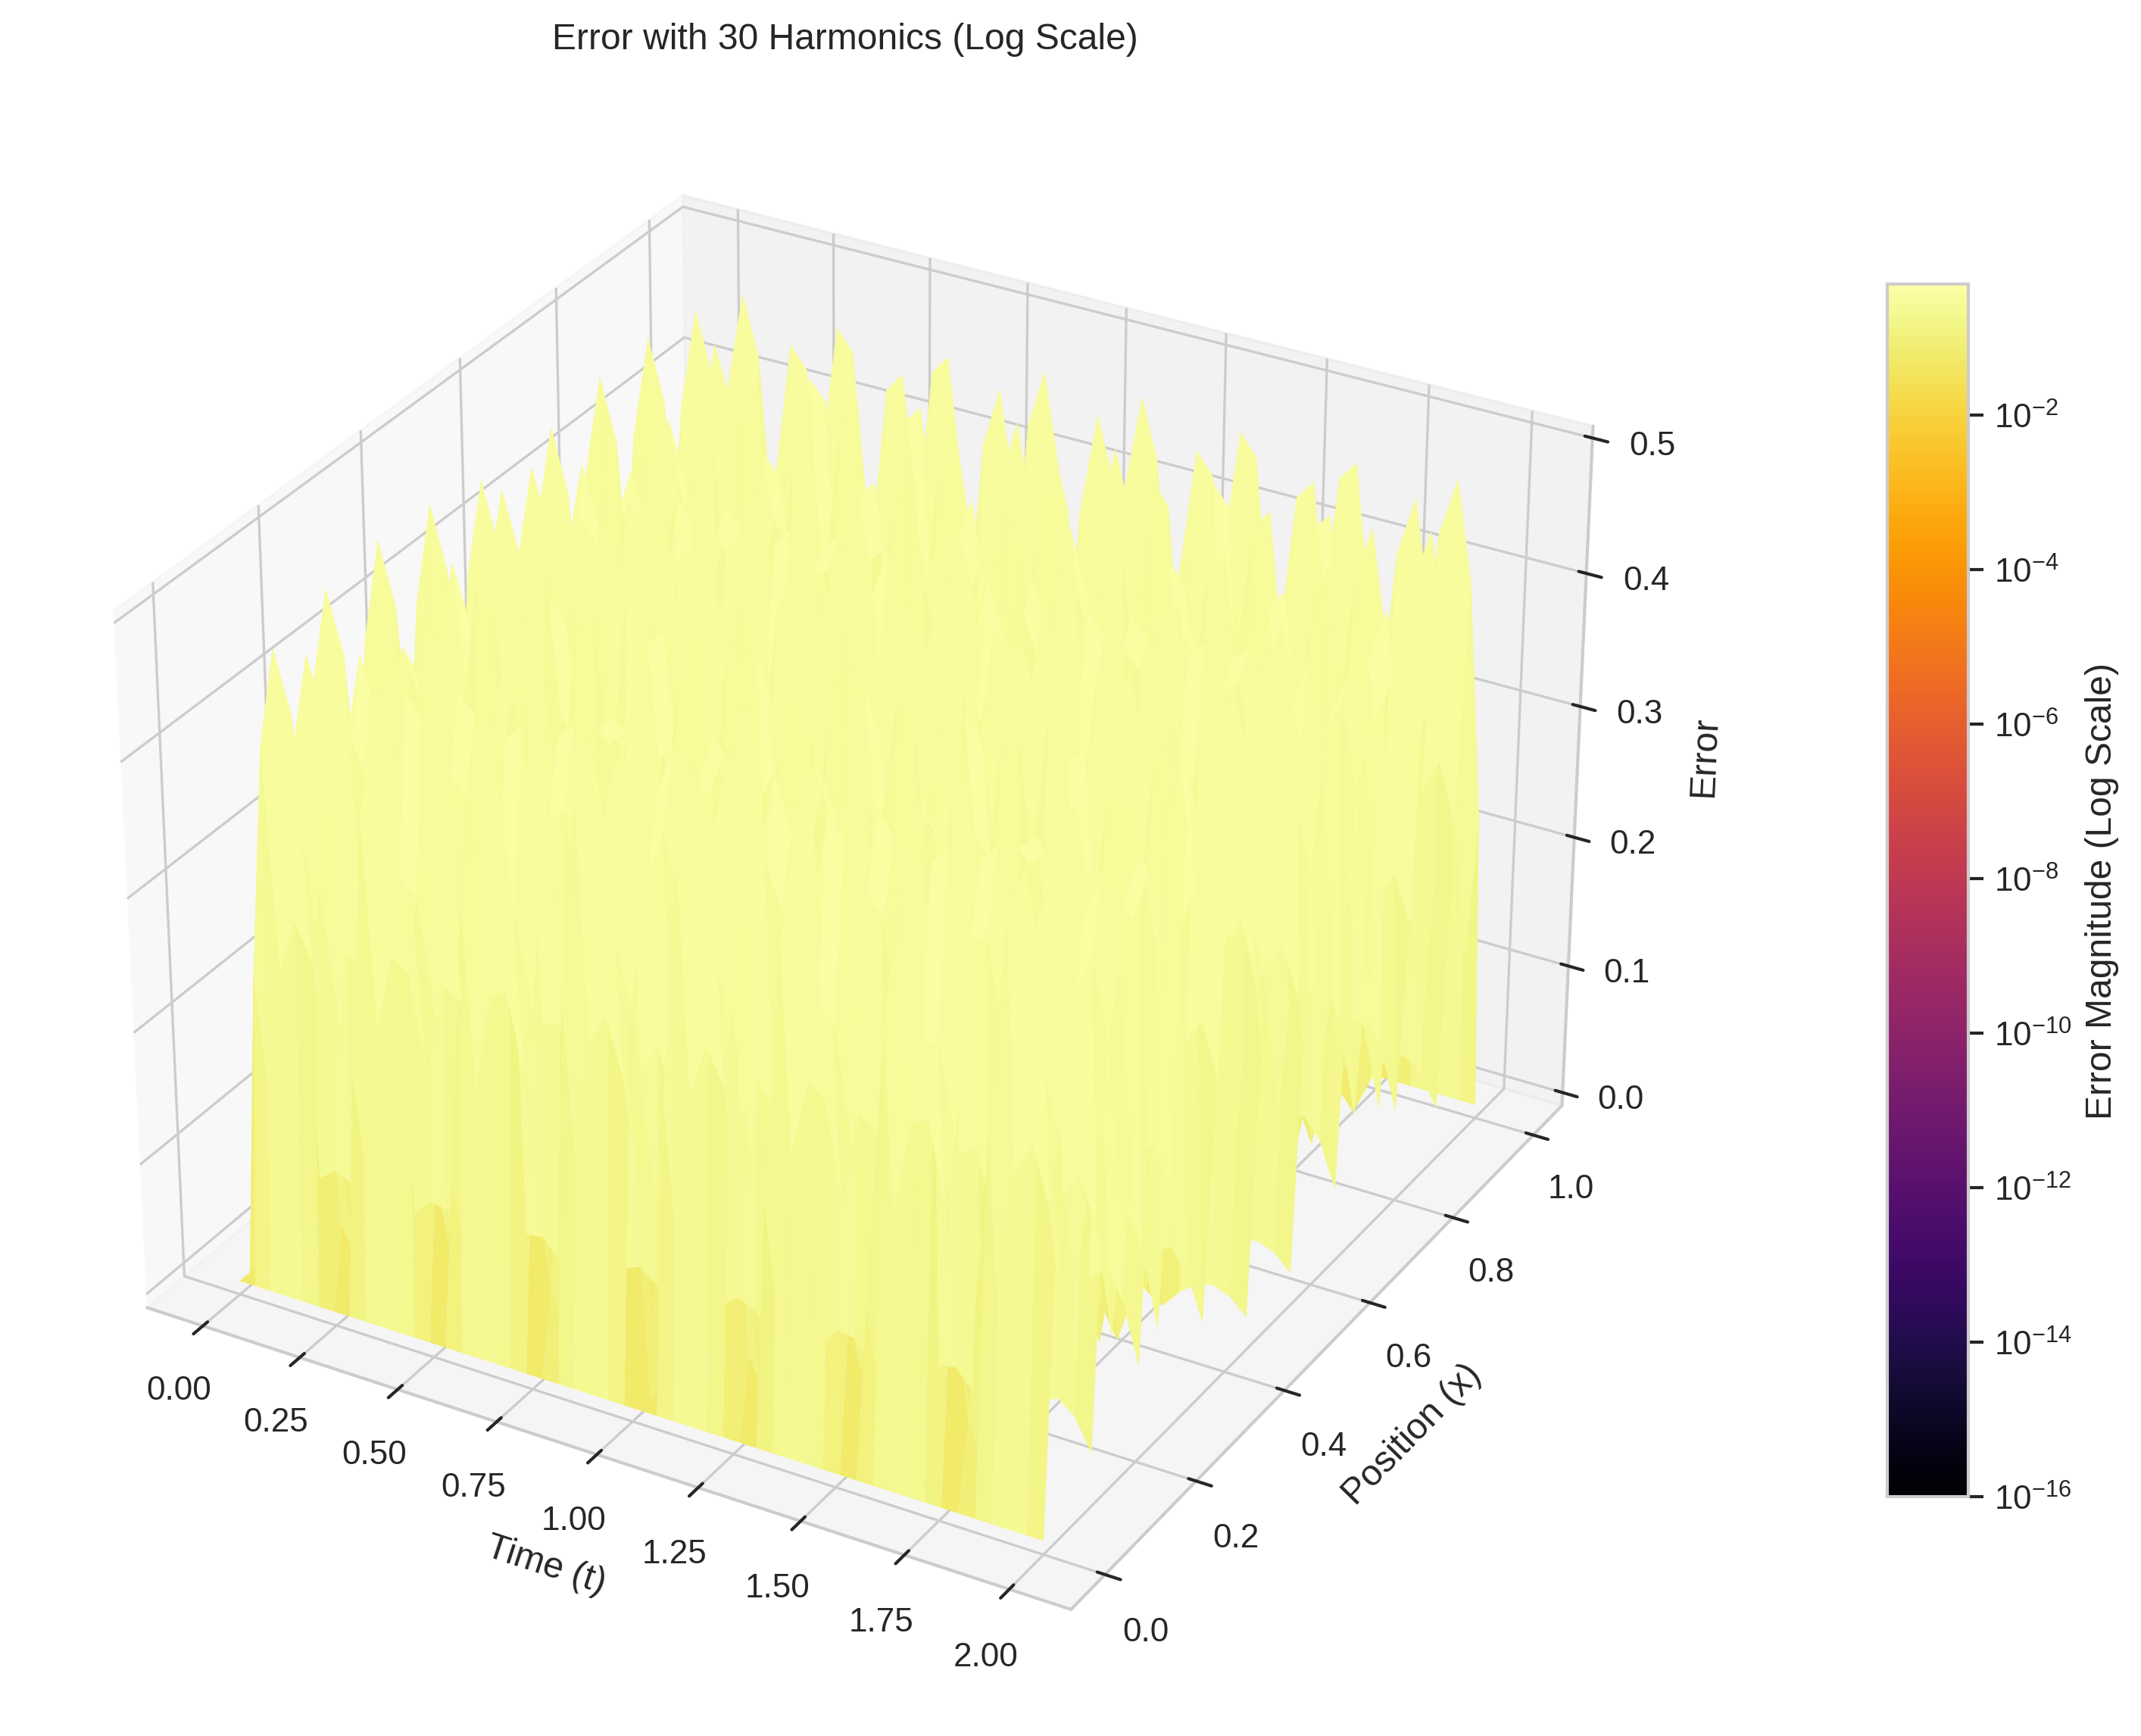
\includegraphics[width=\textwidth]{figures/3d_comparison_error_30h.png}
        \caption{30 harmonics}
    \end{subfigure}
    \hfill
    \begin{subfigure}[b]{0.32\textwidth}
        \centering
        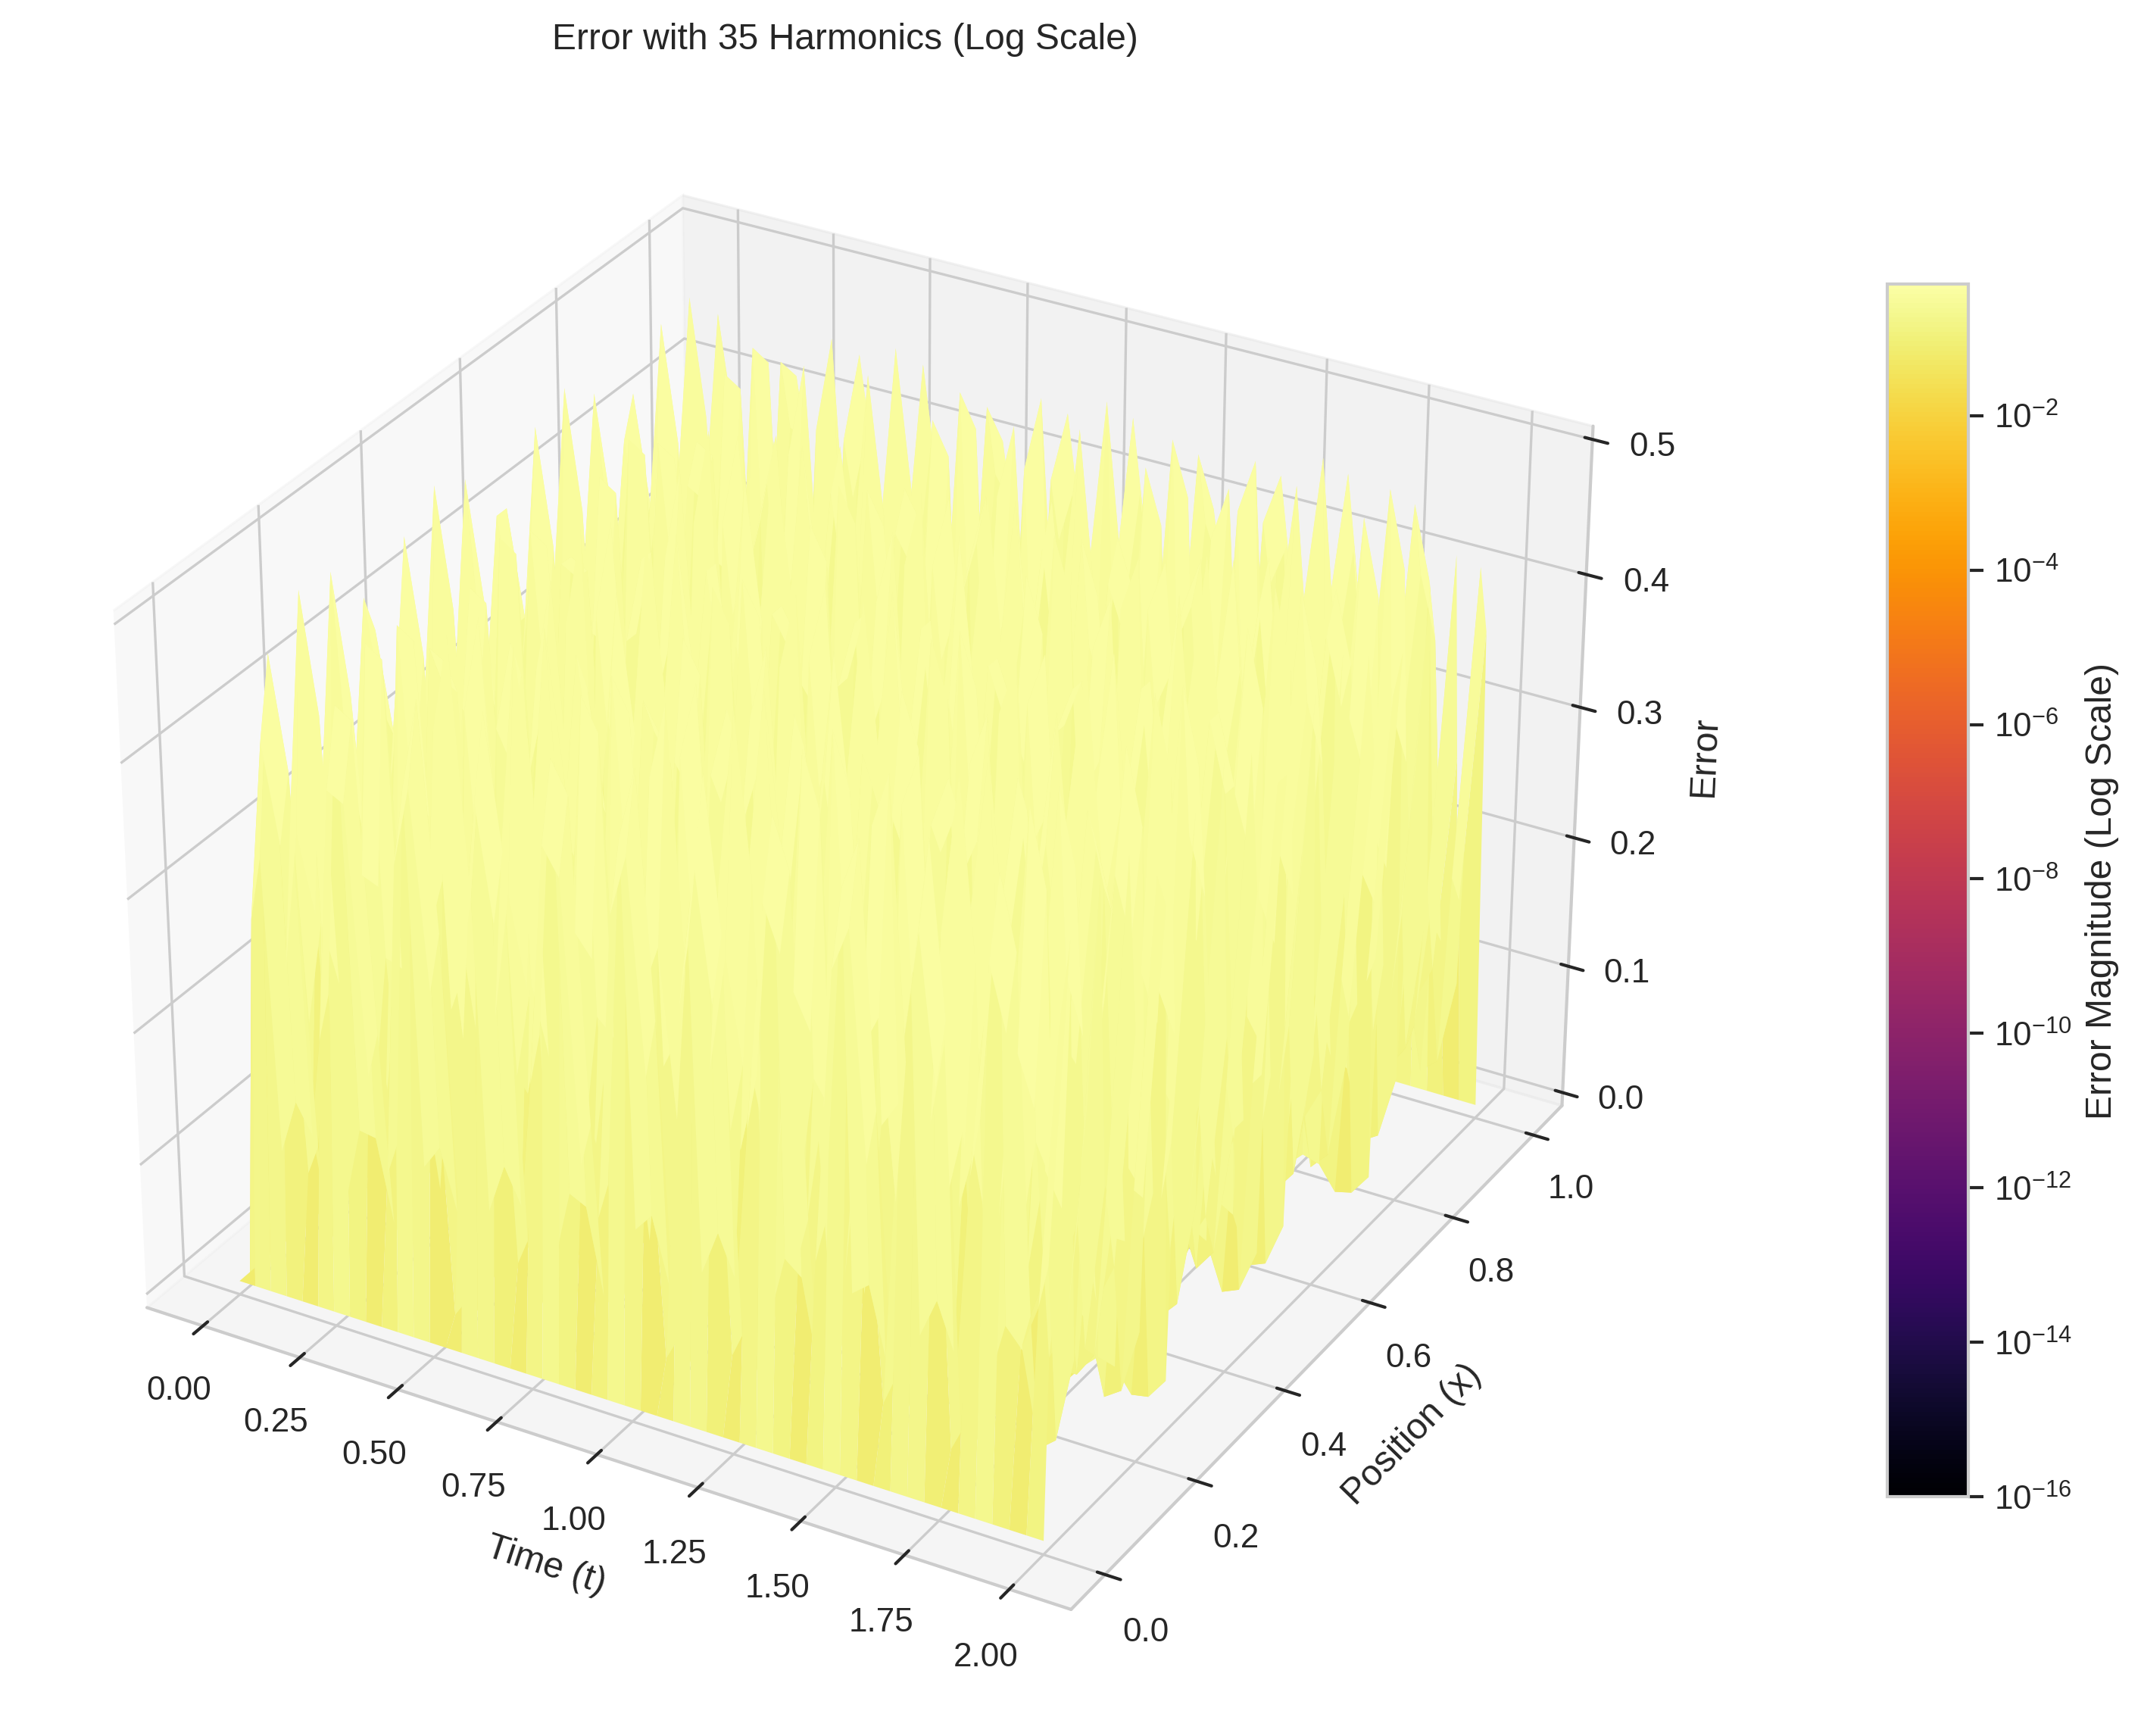
\includegraphics[width=\textwidth]{figures/3d_comparison_error_35h.png}
        \caption{35 harmonics}
    \end{subfigure}
    \caption{Three-dimensional error surfaces for mid-range harmonic configurations showing the transition from acceptable to degraded accuracy.}
    \label{fig:3d_error_mid}
\end{figure}

\begin{figure}[H]
    \centering
    \begin{subfigure}[b]{0.48\textwidth}
        \centering
        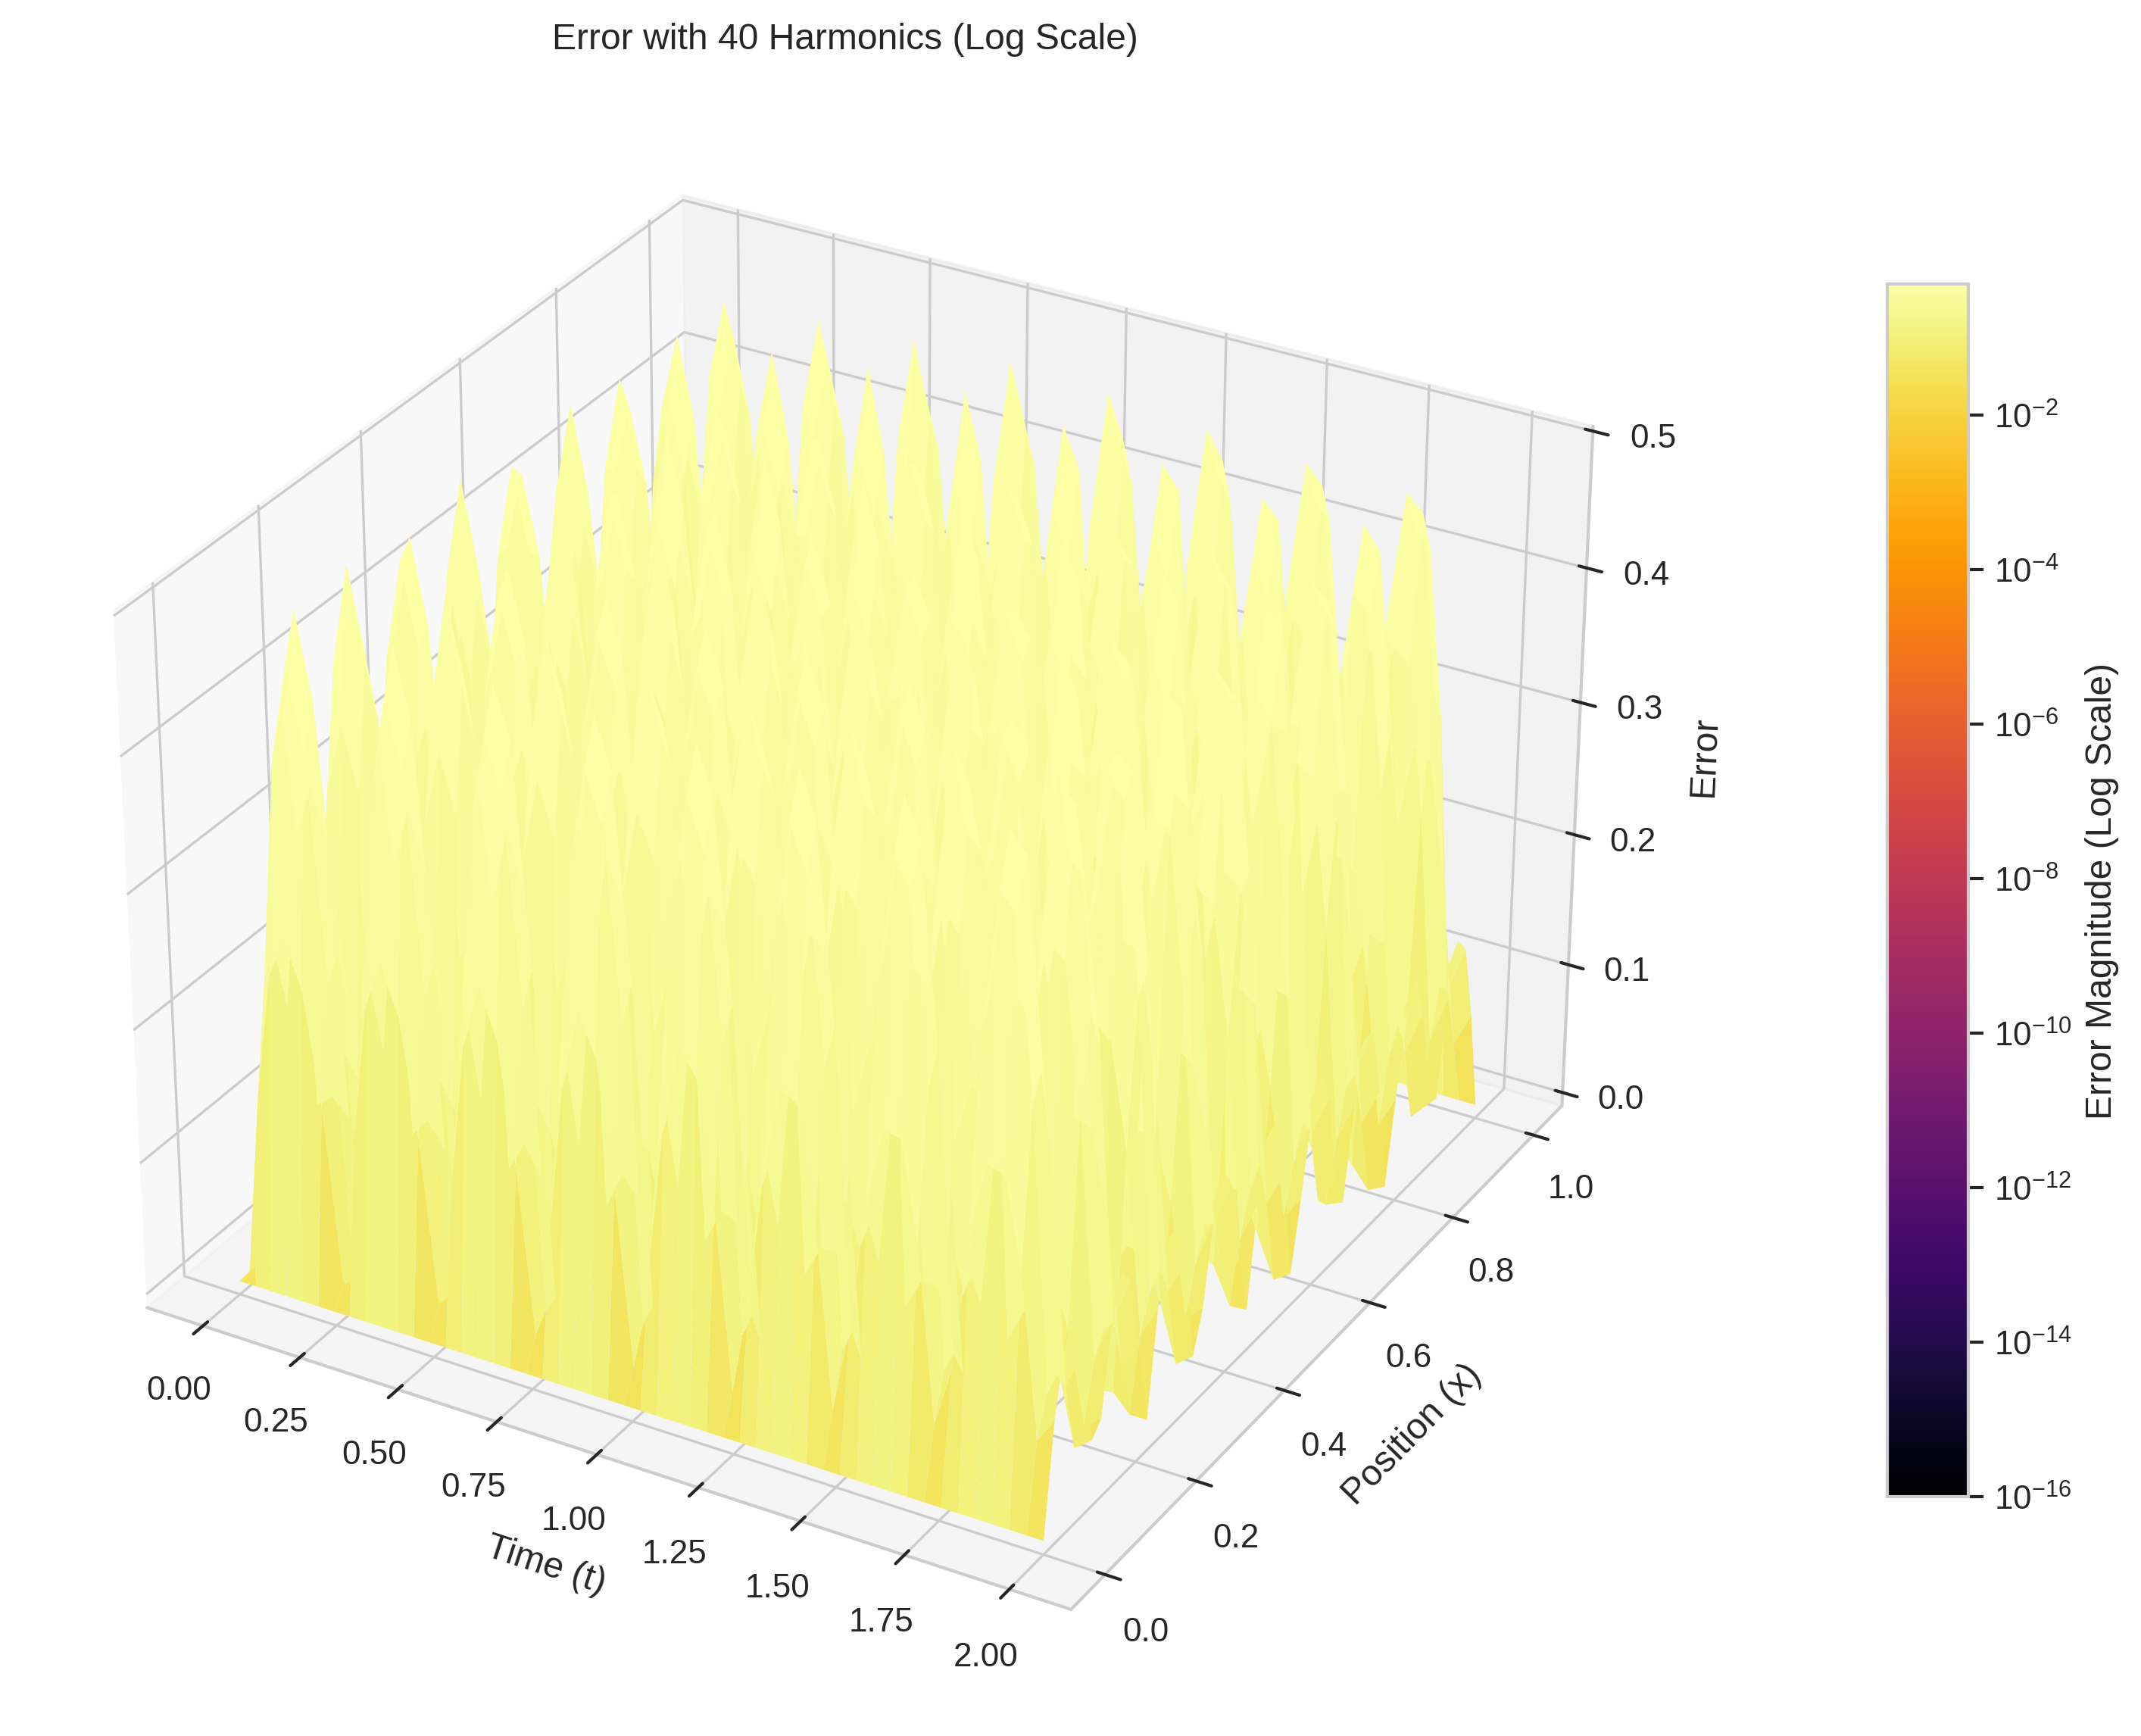
\includegraphics[width=\textwidth]{figures/3d_comparison_error_40h.png}
        \caption{40 harmonics}
    \end{subfigure}
    \hfill
    \begin{subfigure}[b]{0.48\textwidth}
        \centering
        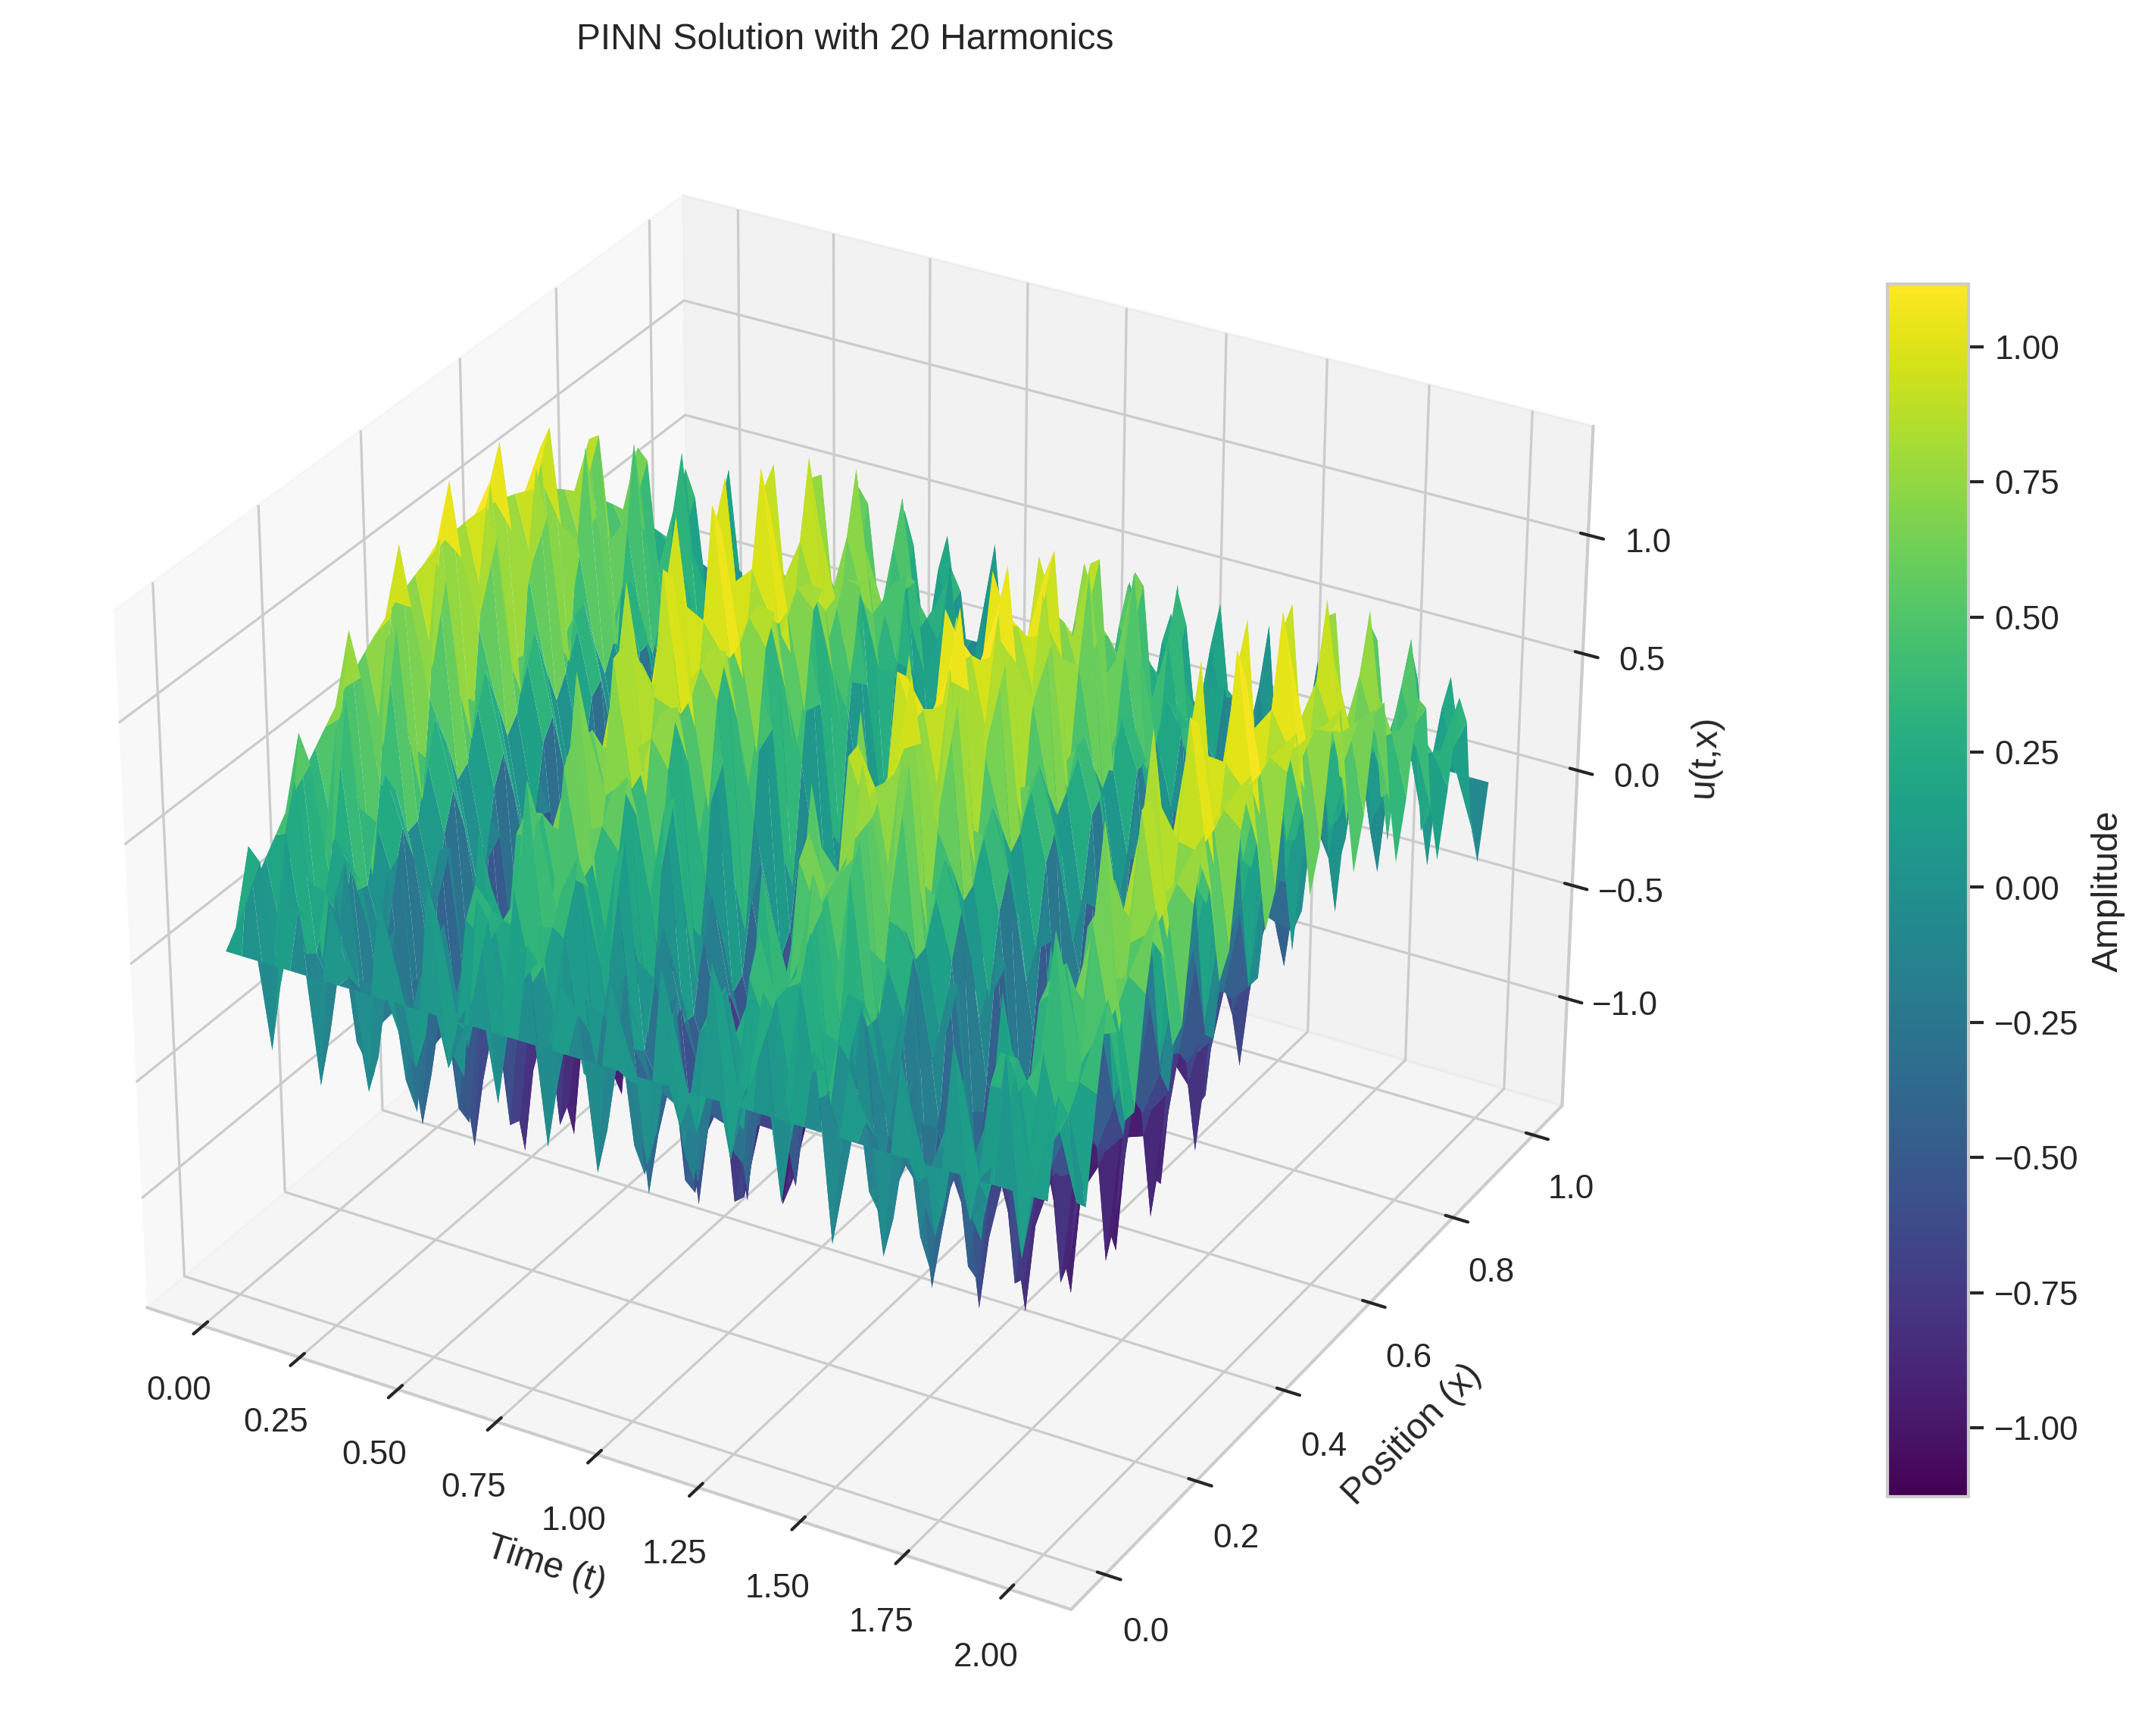
\includegraphics[width=\textwidth]{figures/3d_comparison_pinn_solution_20h.png}
        \caption{20 harmonics solution}
    \end{subfigure}
    \caption{High harmonic error surface and intermediate harmonic solution profile.}
    \label{fig:3d_high_error}
\end{figure}

\subsection{Additional 3D PINN Solutions}

\begin{figure}[H]
    \centering
    \begin{subfigure}[b]{0.32\textwidth}
        \centering
        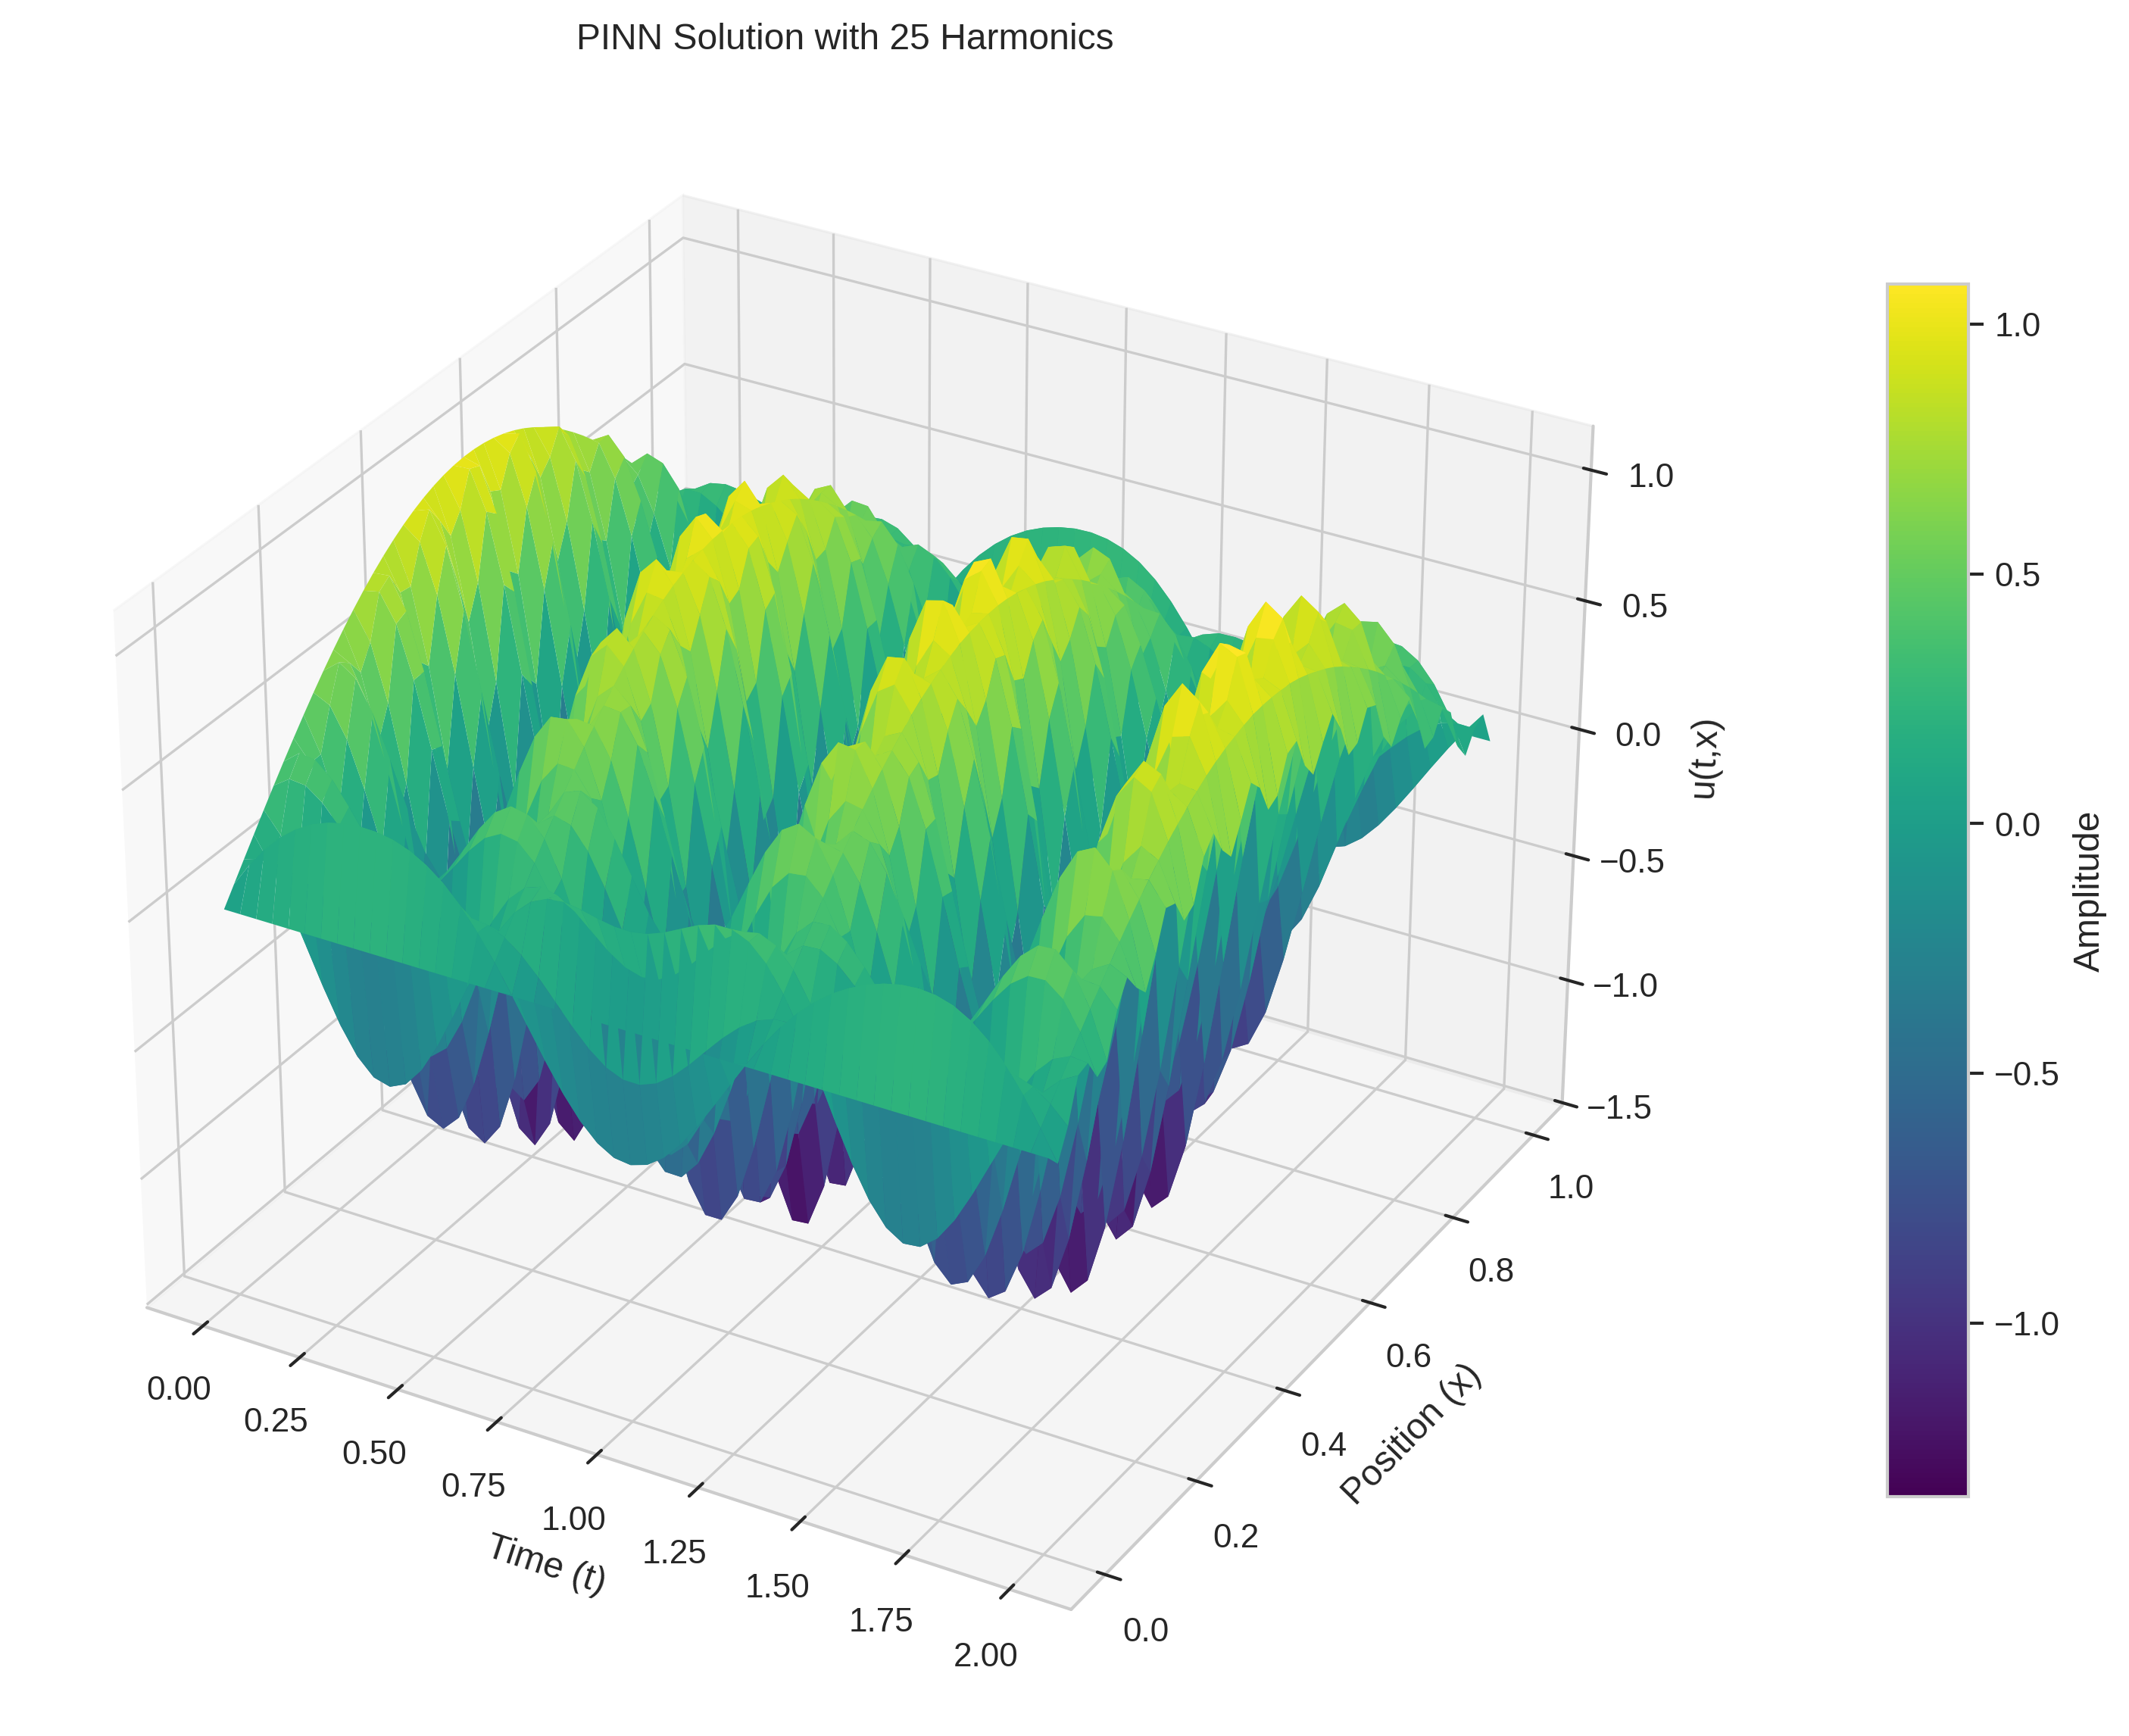
\includegraphics[width=\textwidth]{figures/3d_comparison_pinn_solution_25h.png}
        \caption{25 harmonics}
    \end{subfigure}
    \hfill
    \begin{subfigure}[b]{0.32\textwidth}
        \centering
        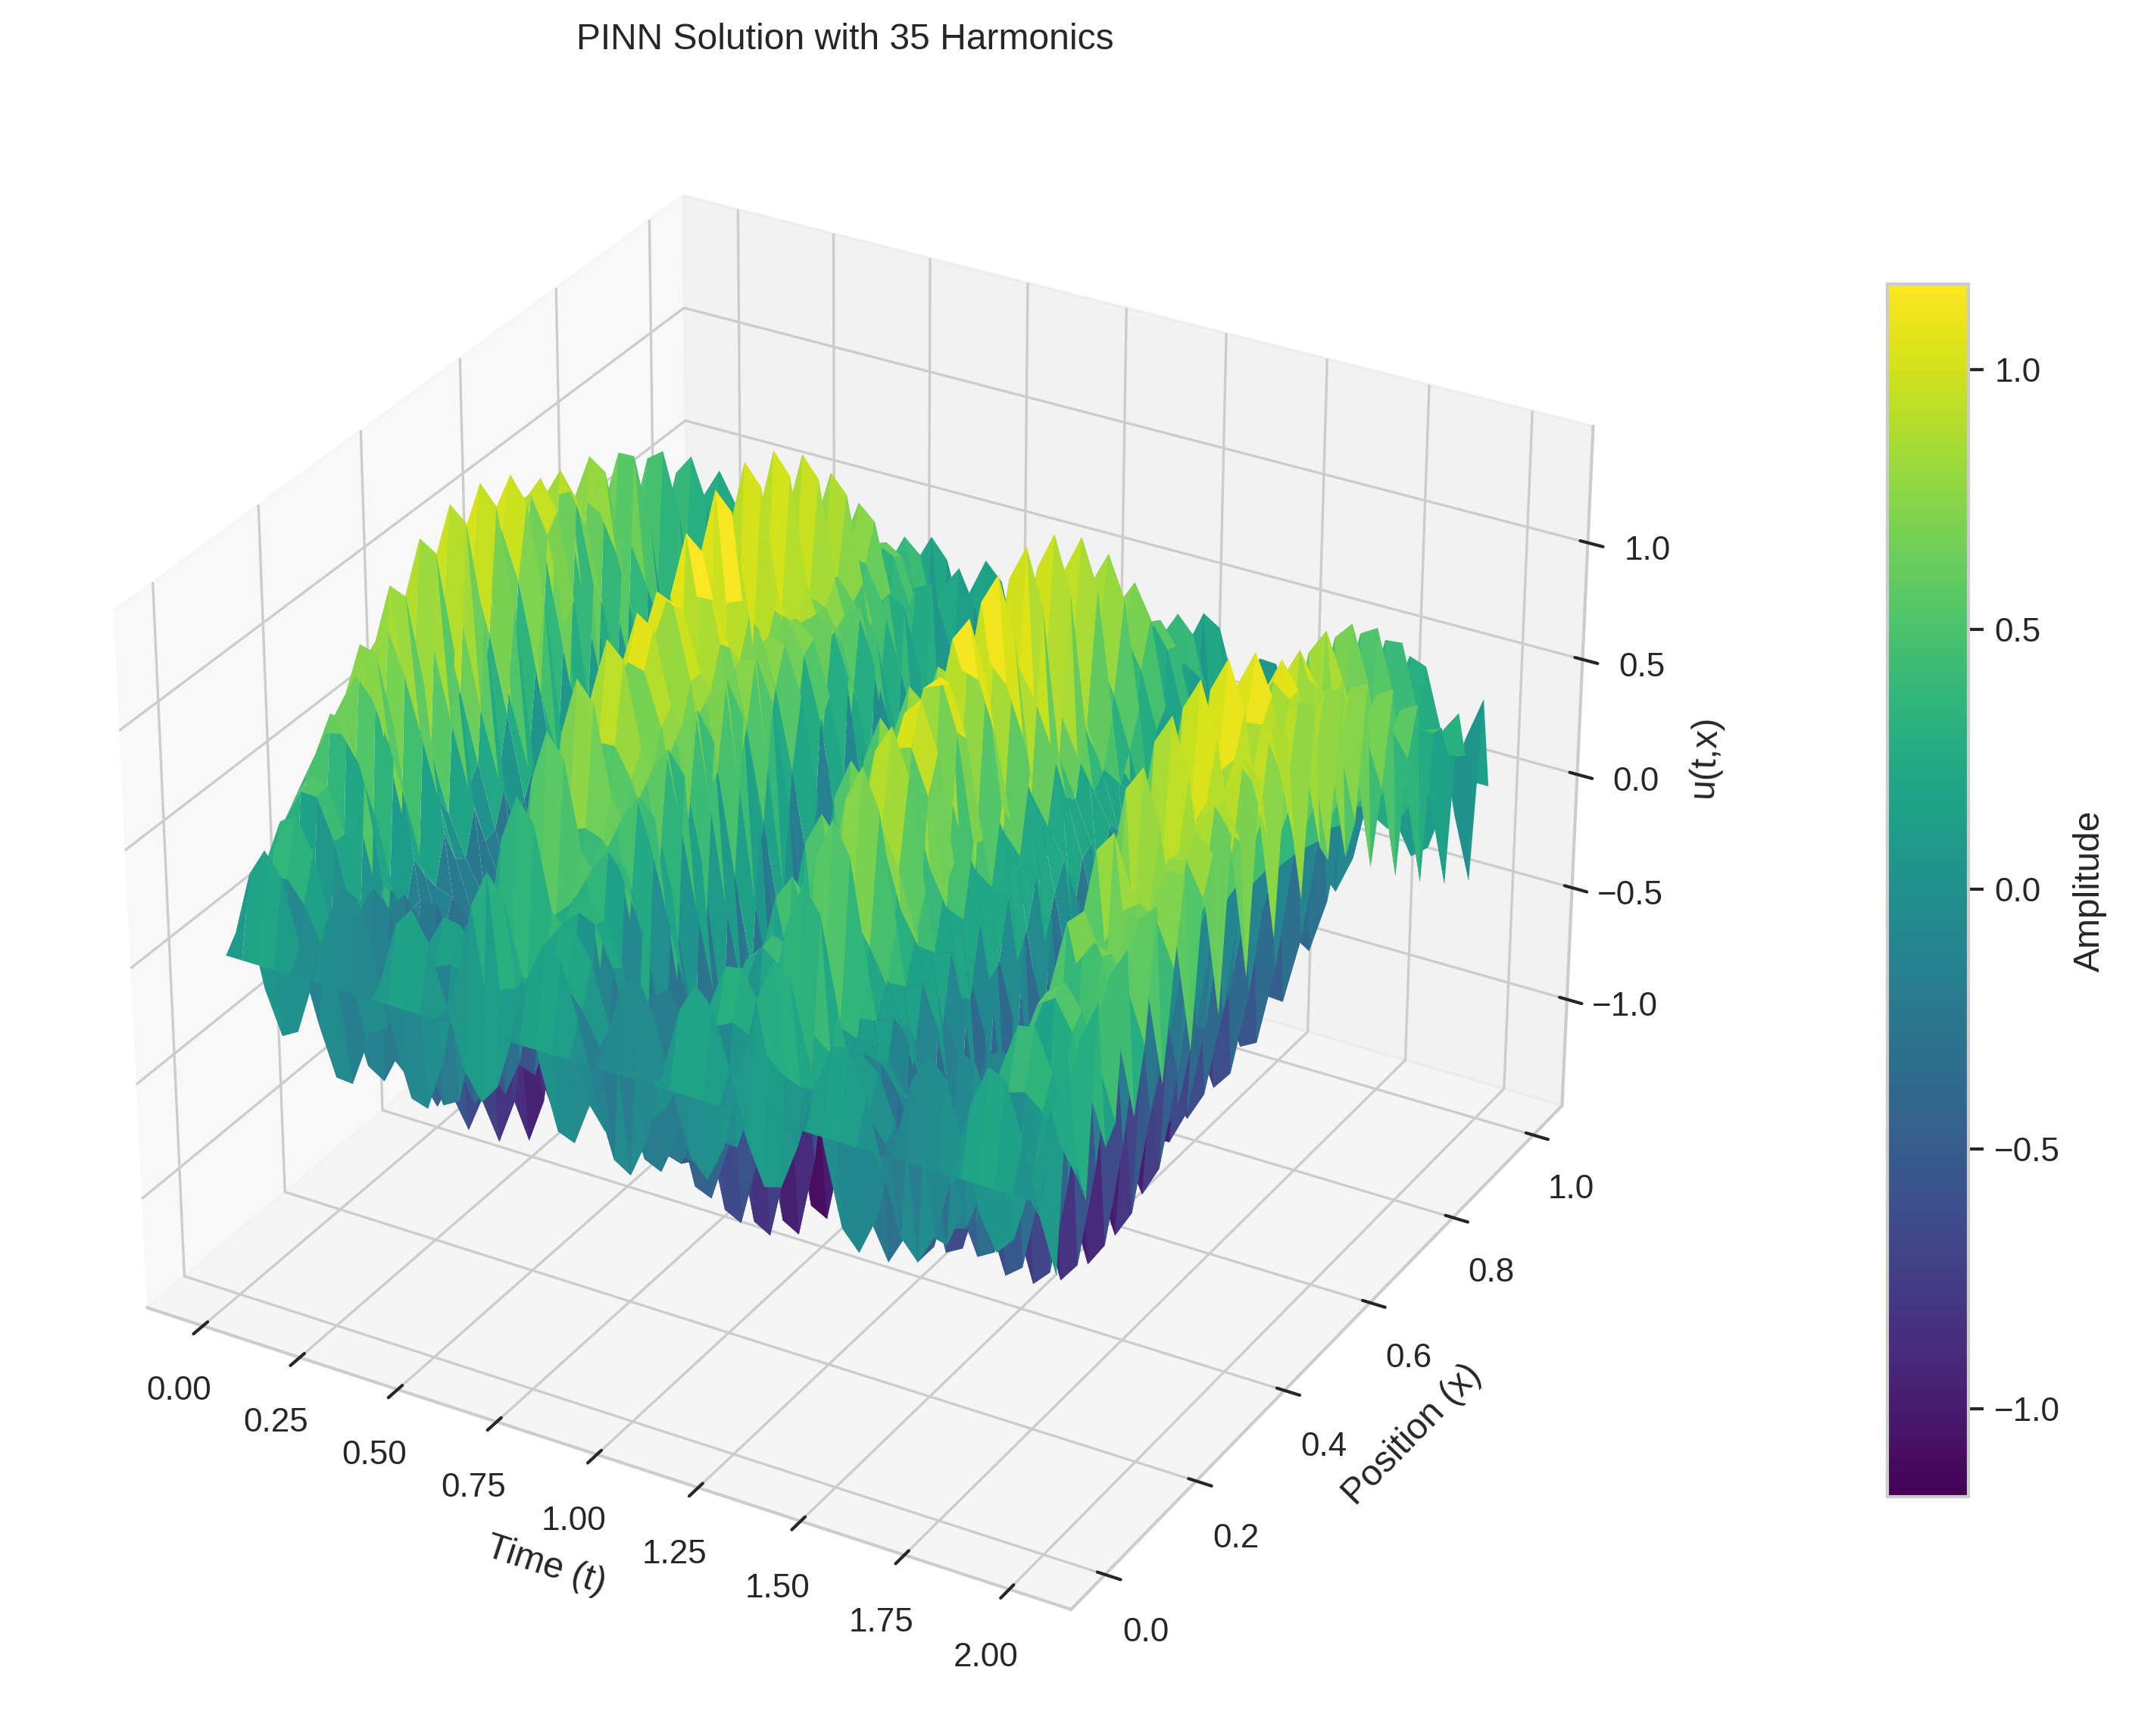
\includegraphics[width=\textwidth]{figures/3d_comparison_pinn_solution_35h.png}
        \caption{35 harmonics}
    \end{subfigure}
    \hfill
    \begin{subfigure}[b]{0.32\textwidth}
        \centering
        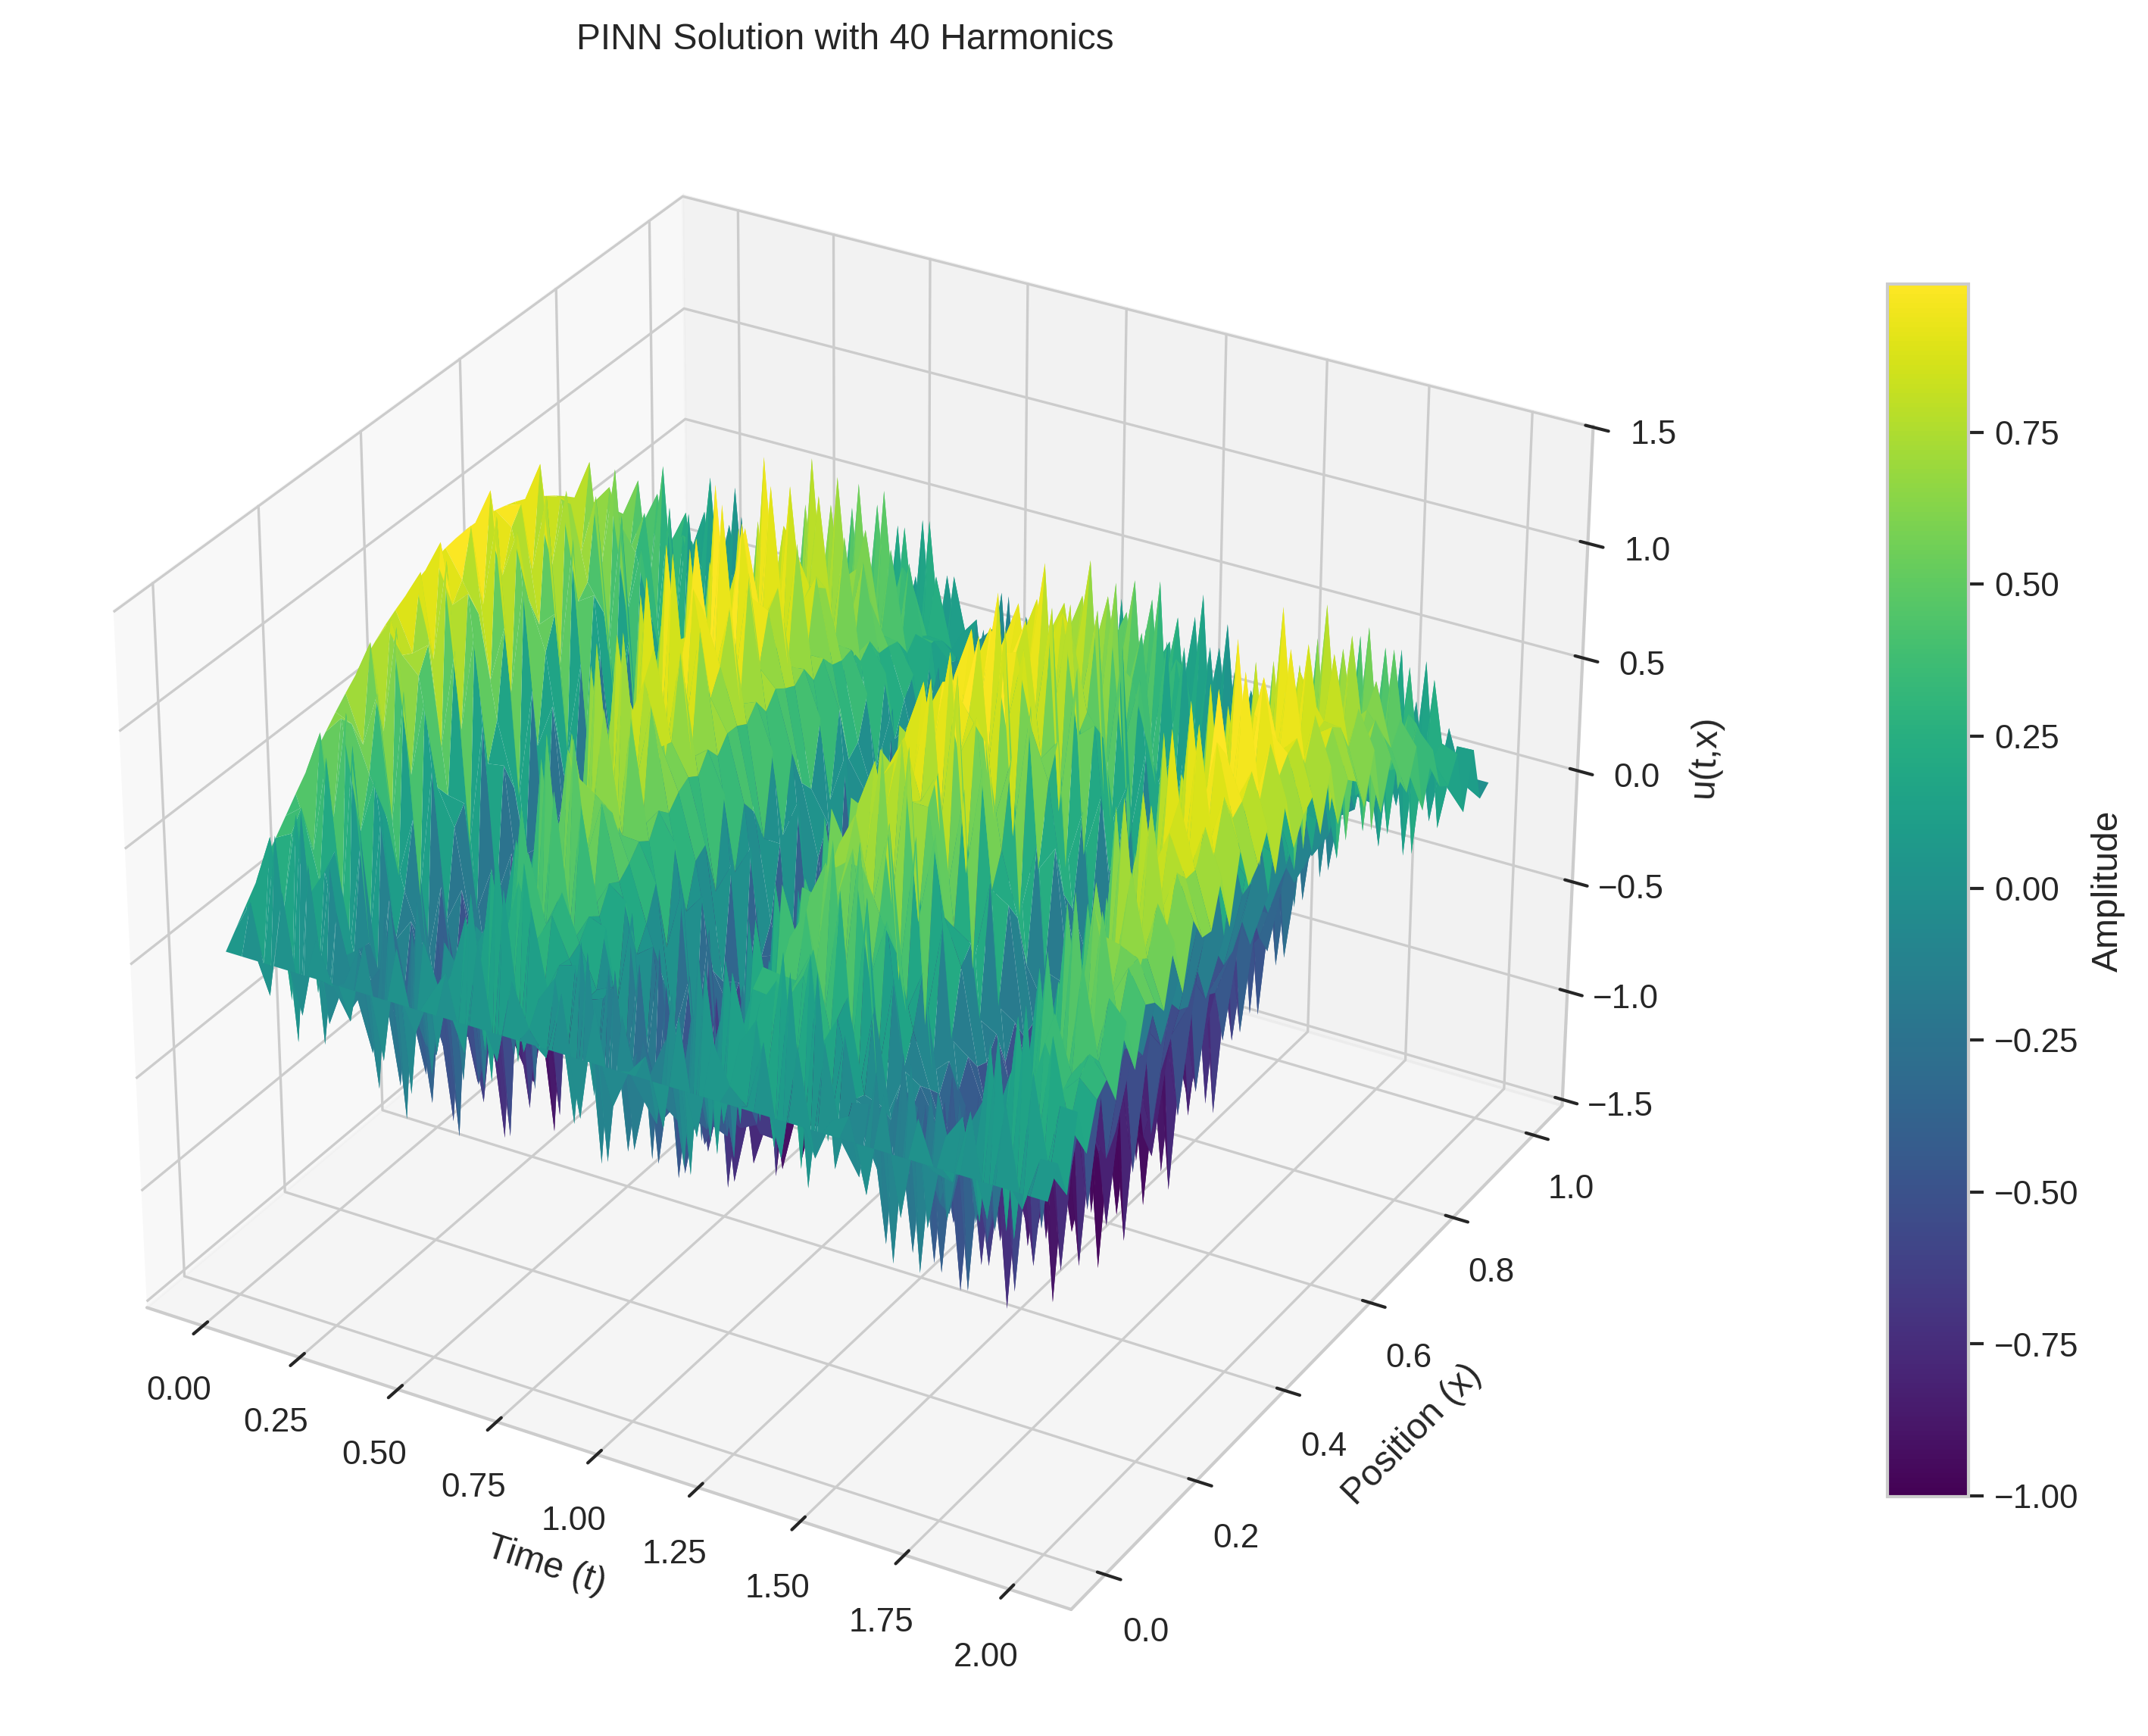
\includegraphics[width=\textwidth]{figures/3d_comparison_pinn_solution_40h.png}
        \caption{40 harmonics}
    \end{subfigure}
    \caption{Three-dimensional PINN solutions for additional harmonic configurations.}
    \label{fig:3d_pinn_additional}
\end{figure}

\begin{figure}[H]
    \centering
    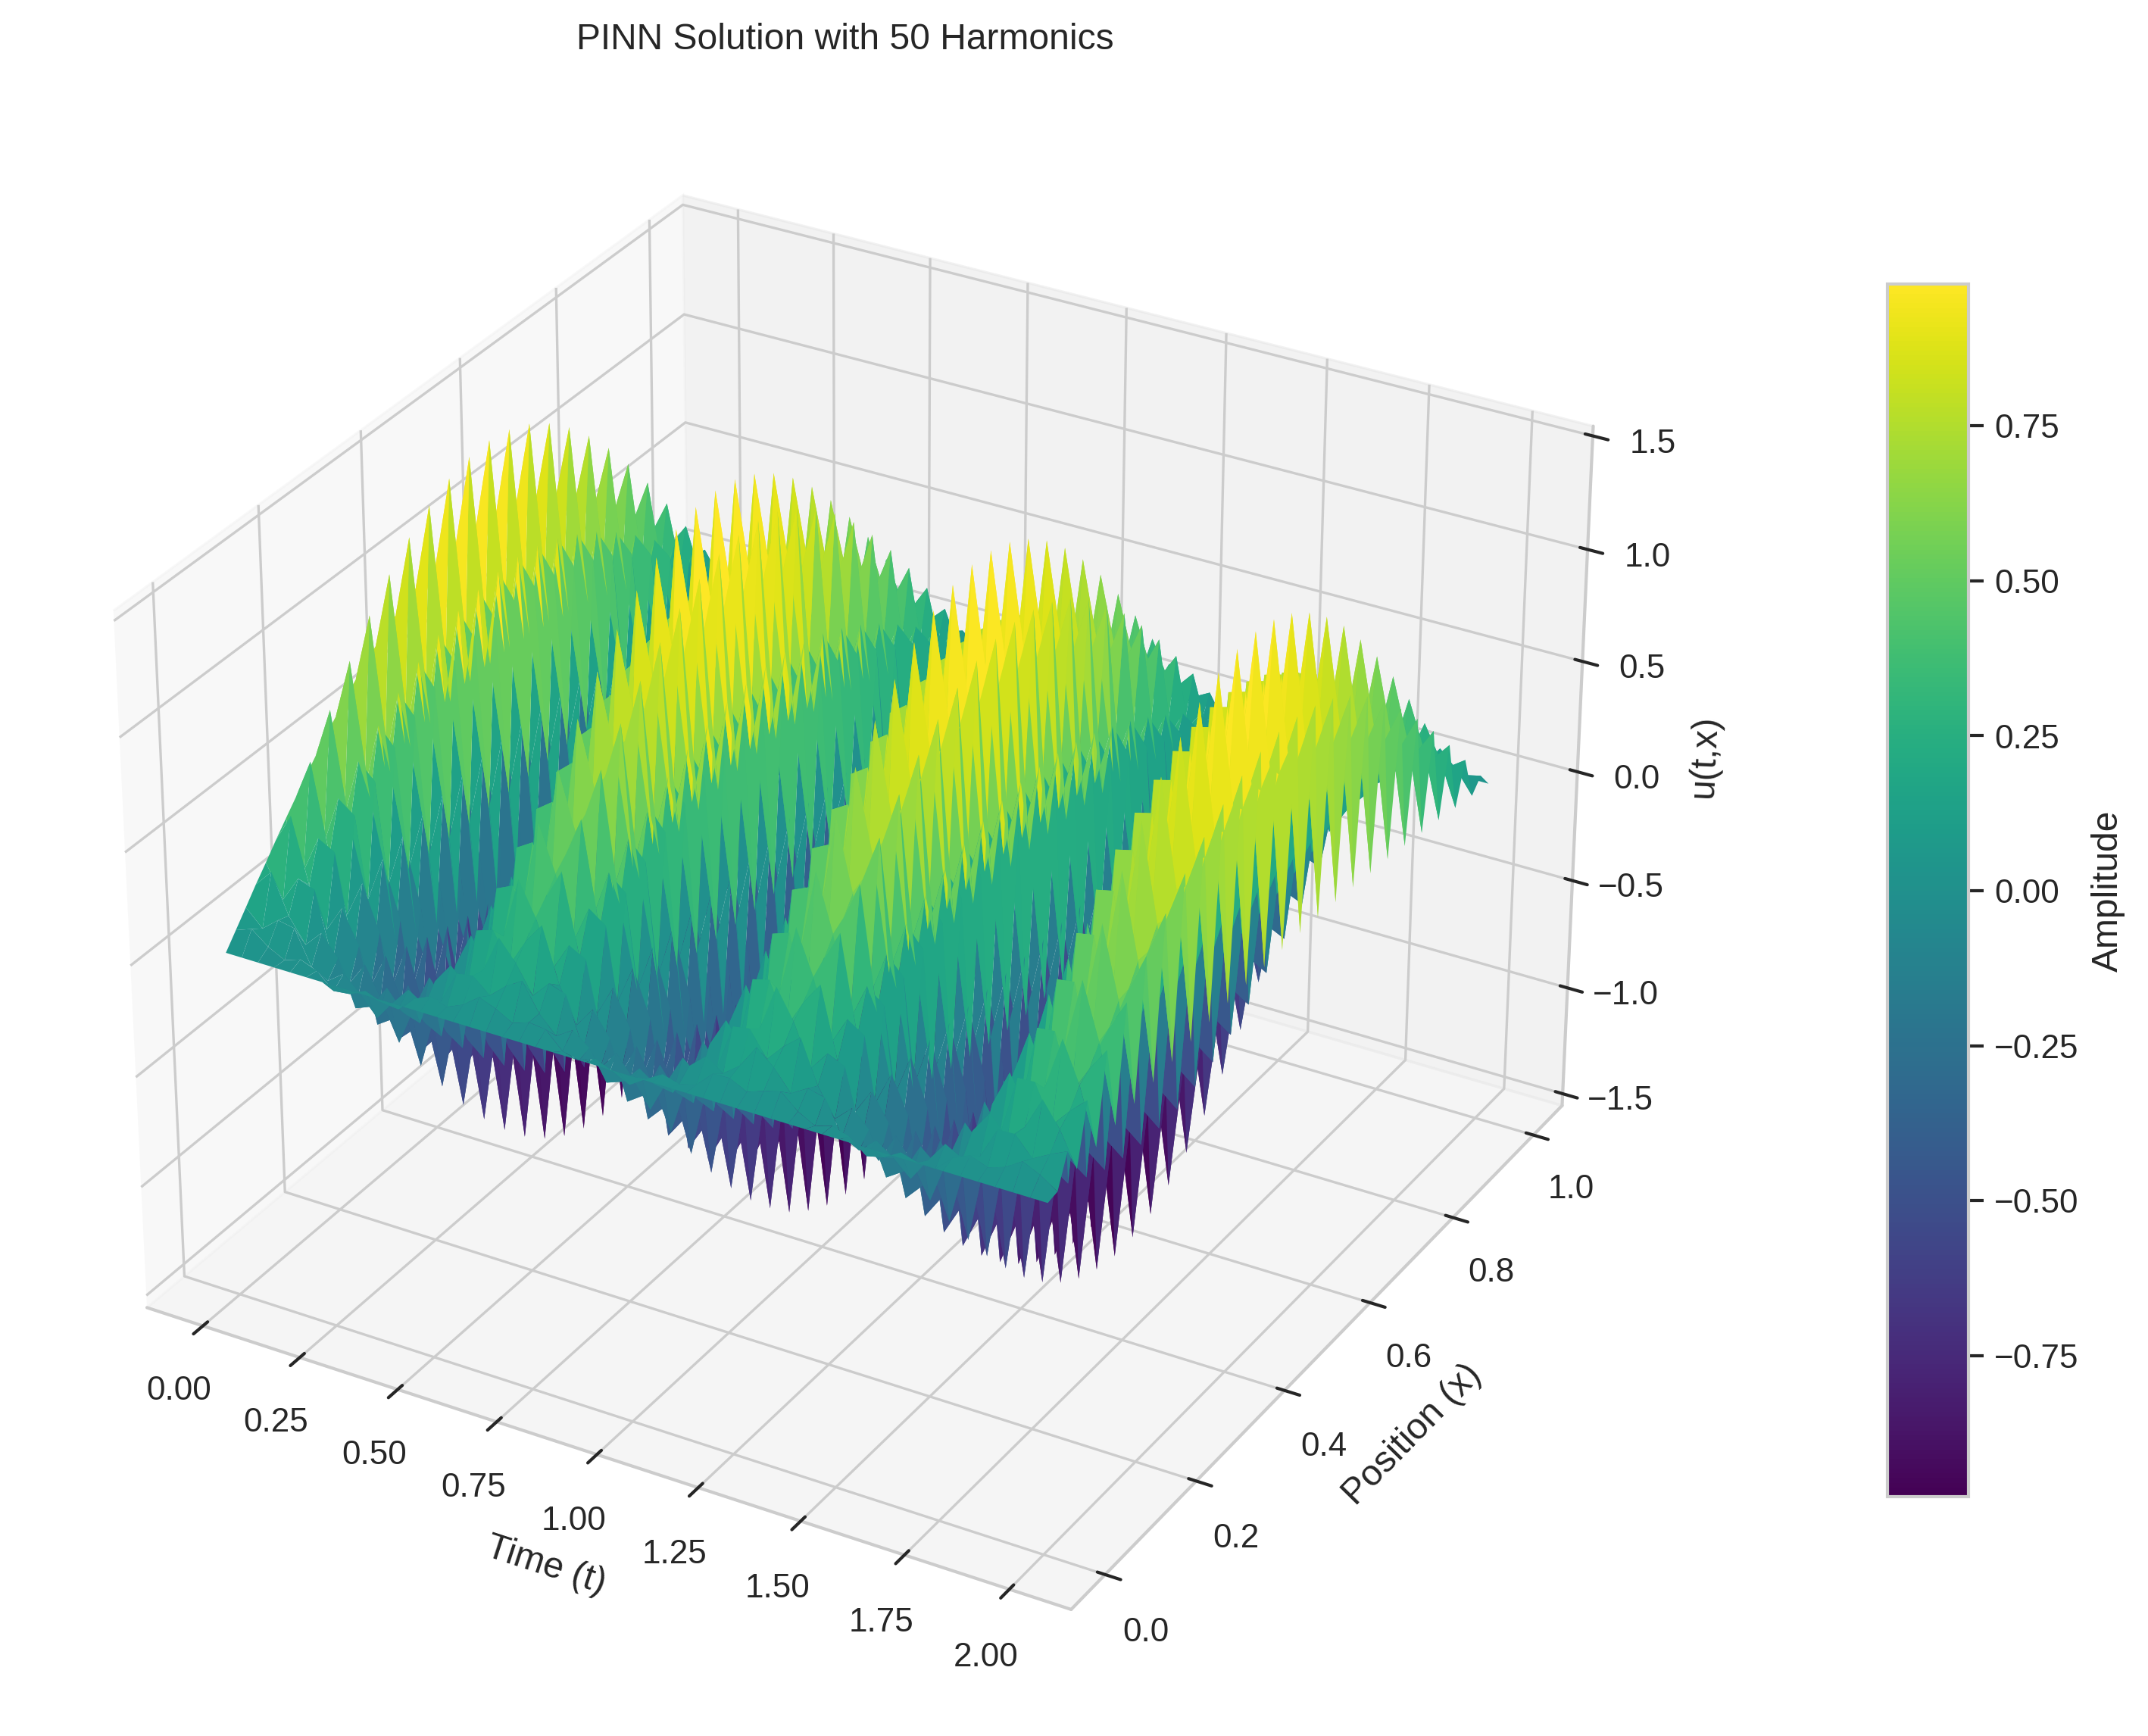
\includegraphics[width=0.6\textwidth]{figures/3d_comparison_pinn_solution_50h.png}
    \caption{PINN solution with 50 harmonics showing severe degradation in solution quality.}
    \label{fig:3d_pinn_50h}
\end{figure}

\subsection{Complete Spatial Slice Analysis}

\begin{figure}[H]
    \centering
    \begin{subfigure}[b]{0.32\textwidth}
        \centering
        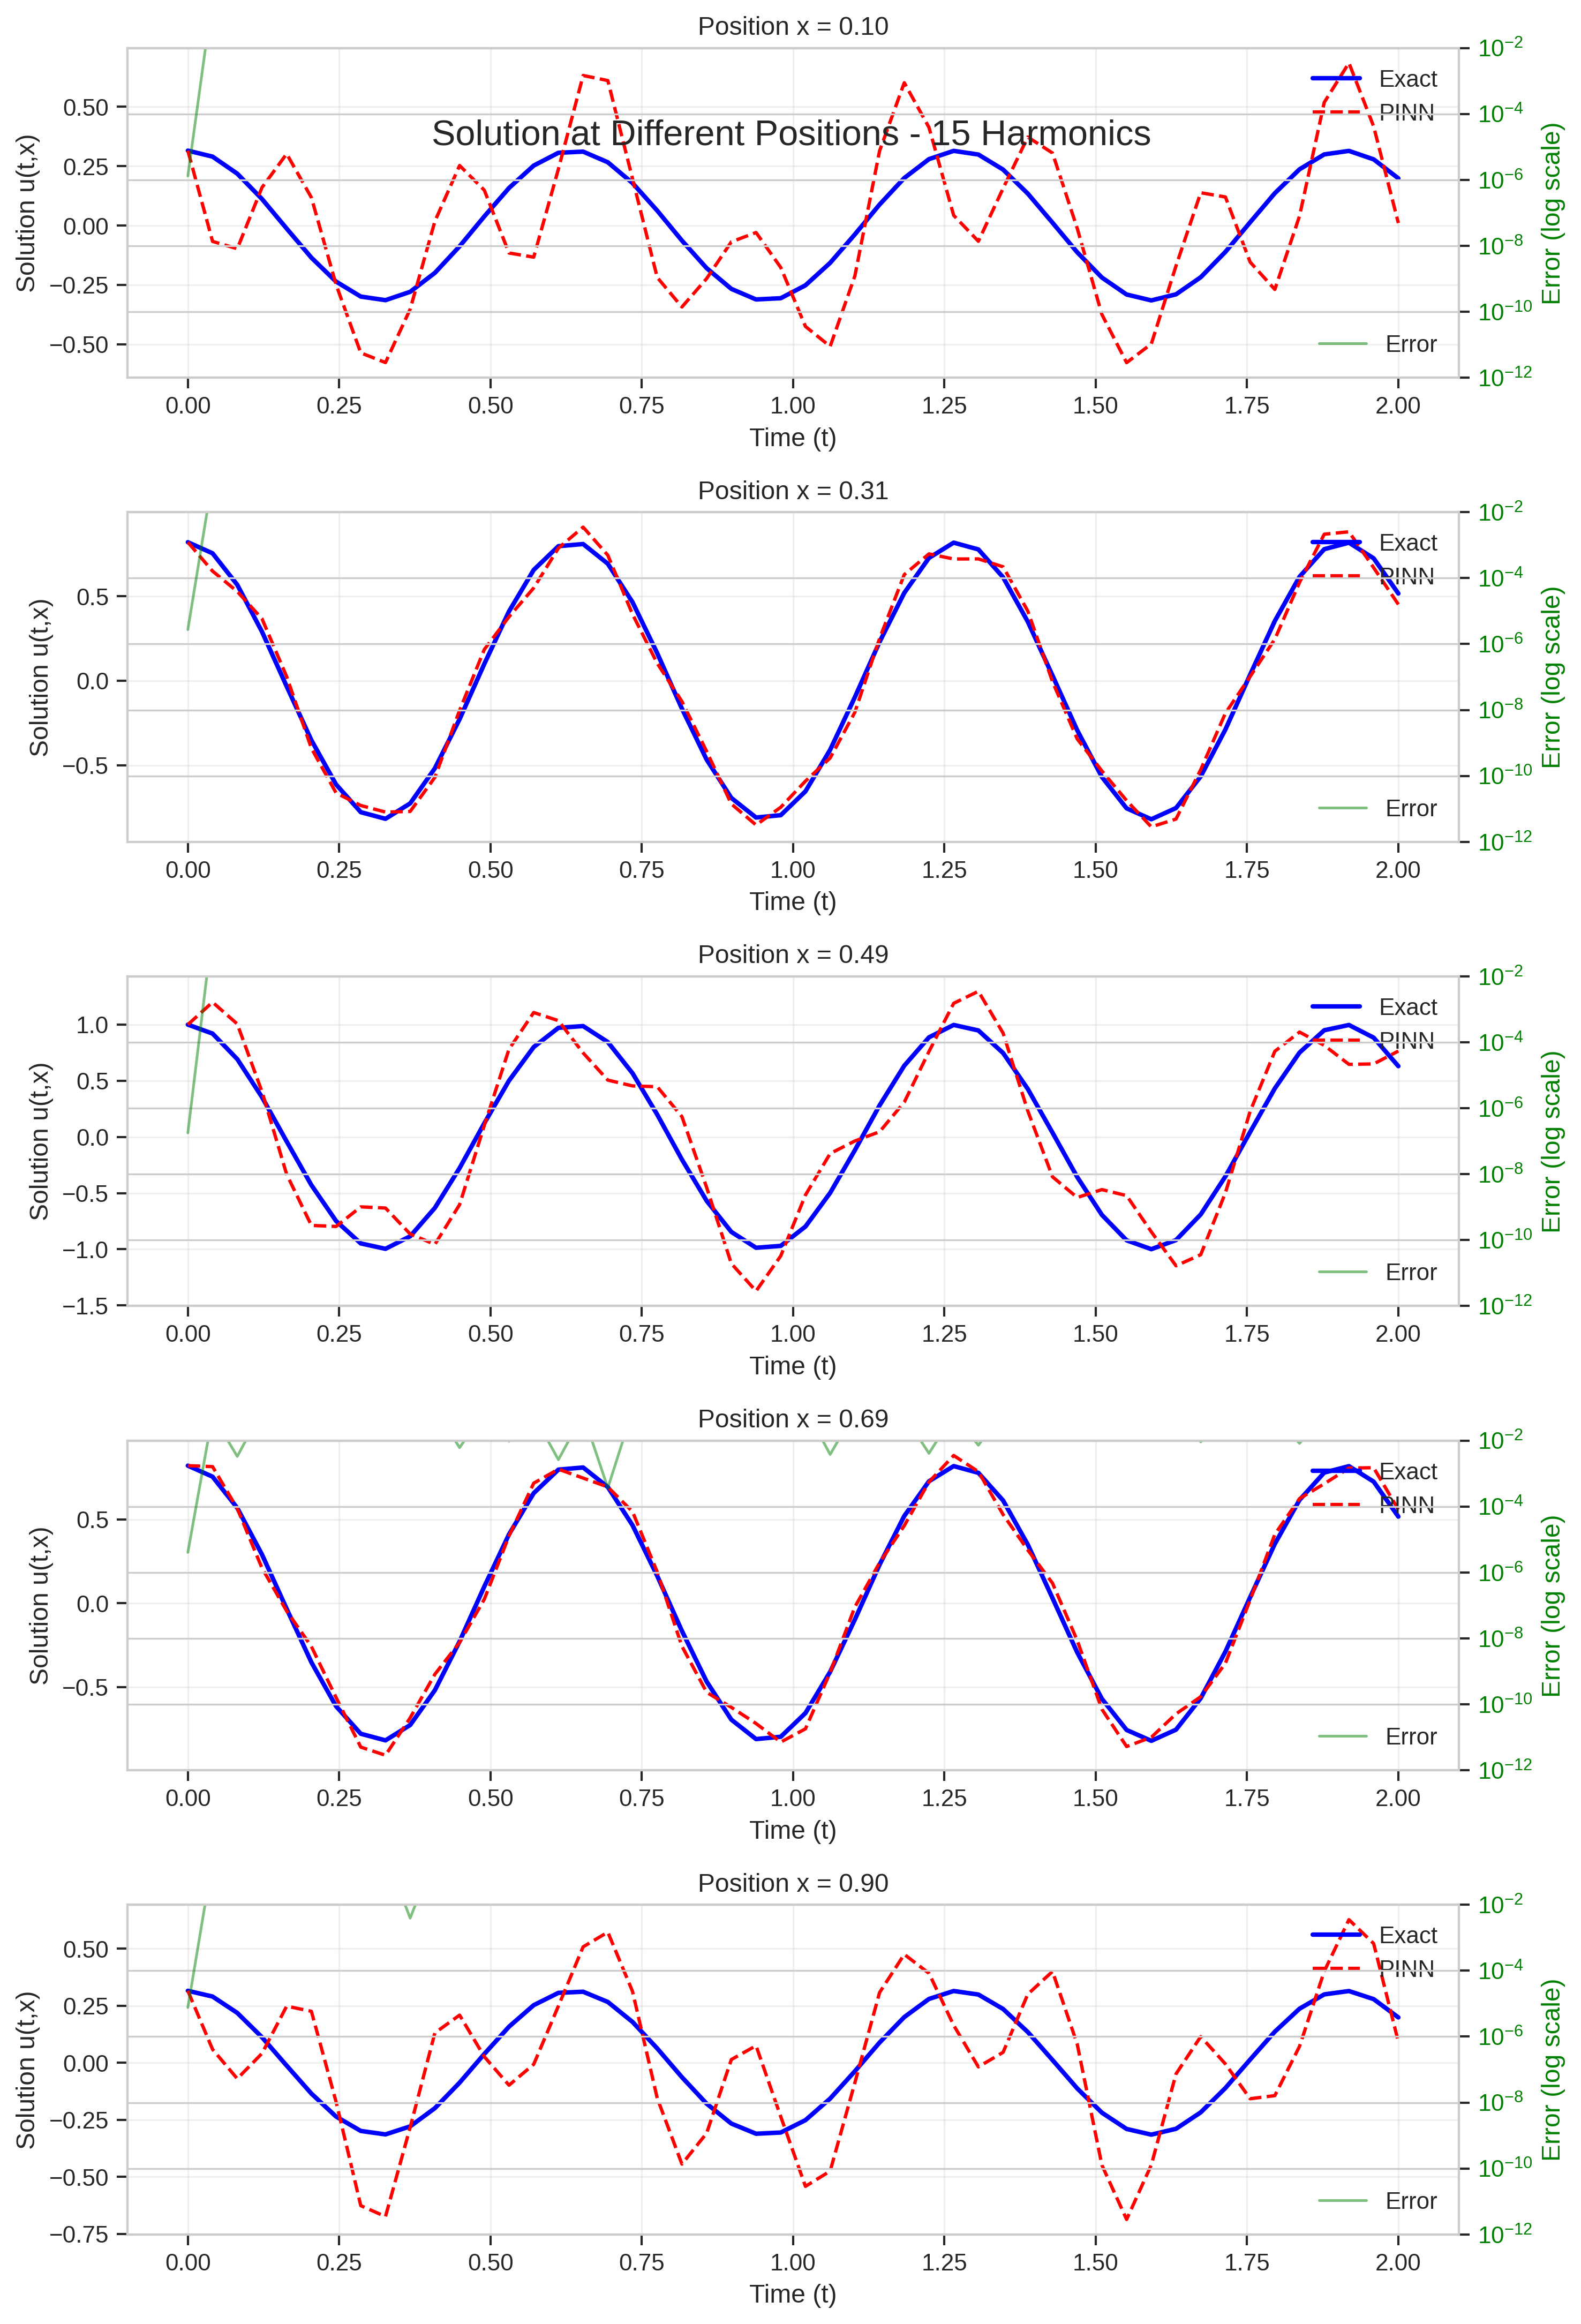
\includegraphics[width=\textwidth]{figures/space_slices_15h.png}
        \caption{15 harmonics}
    \end{subfigure}
    \hfill
    \begin{subfigure}[b]{0.32\textwidth}
        \centering
        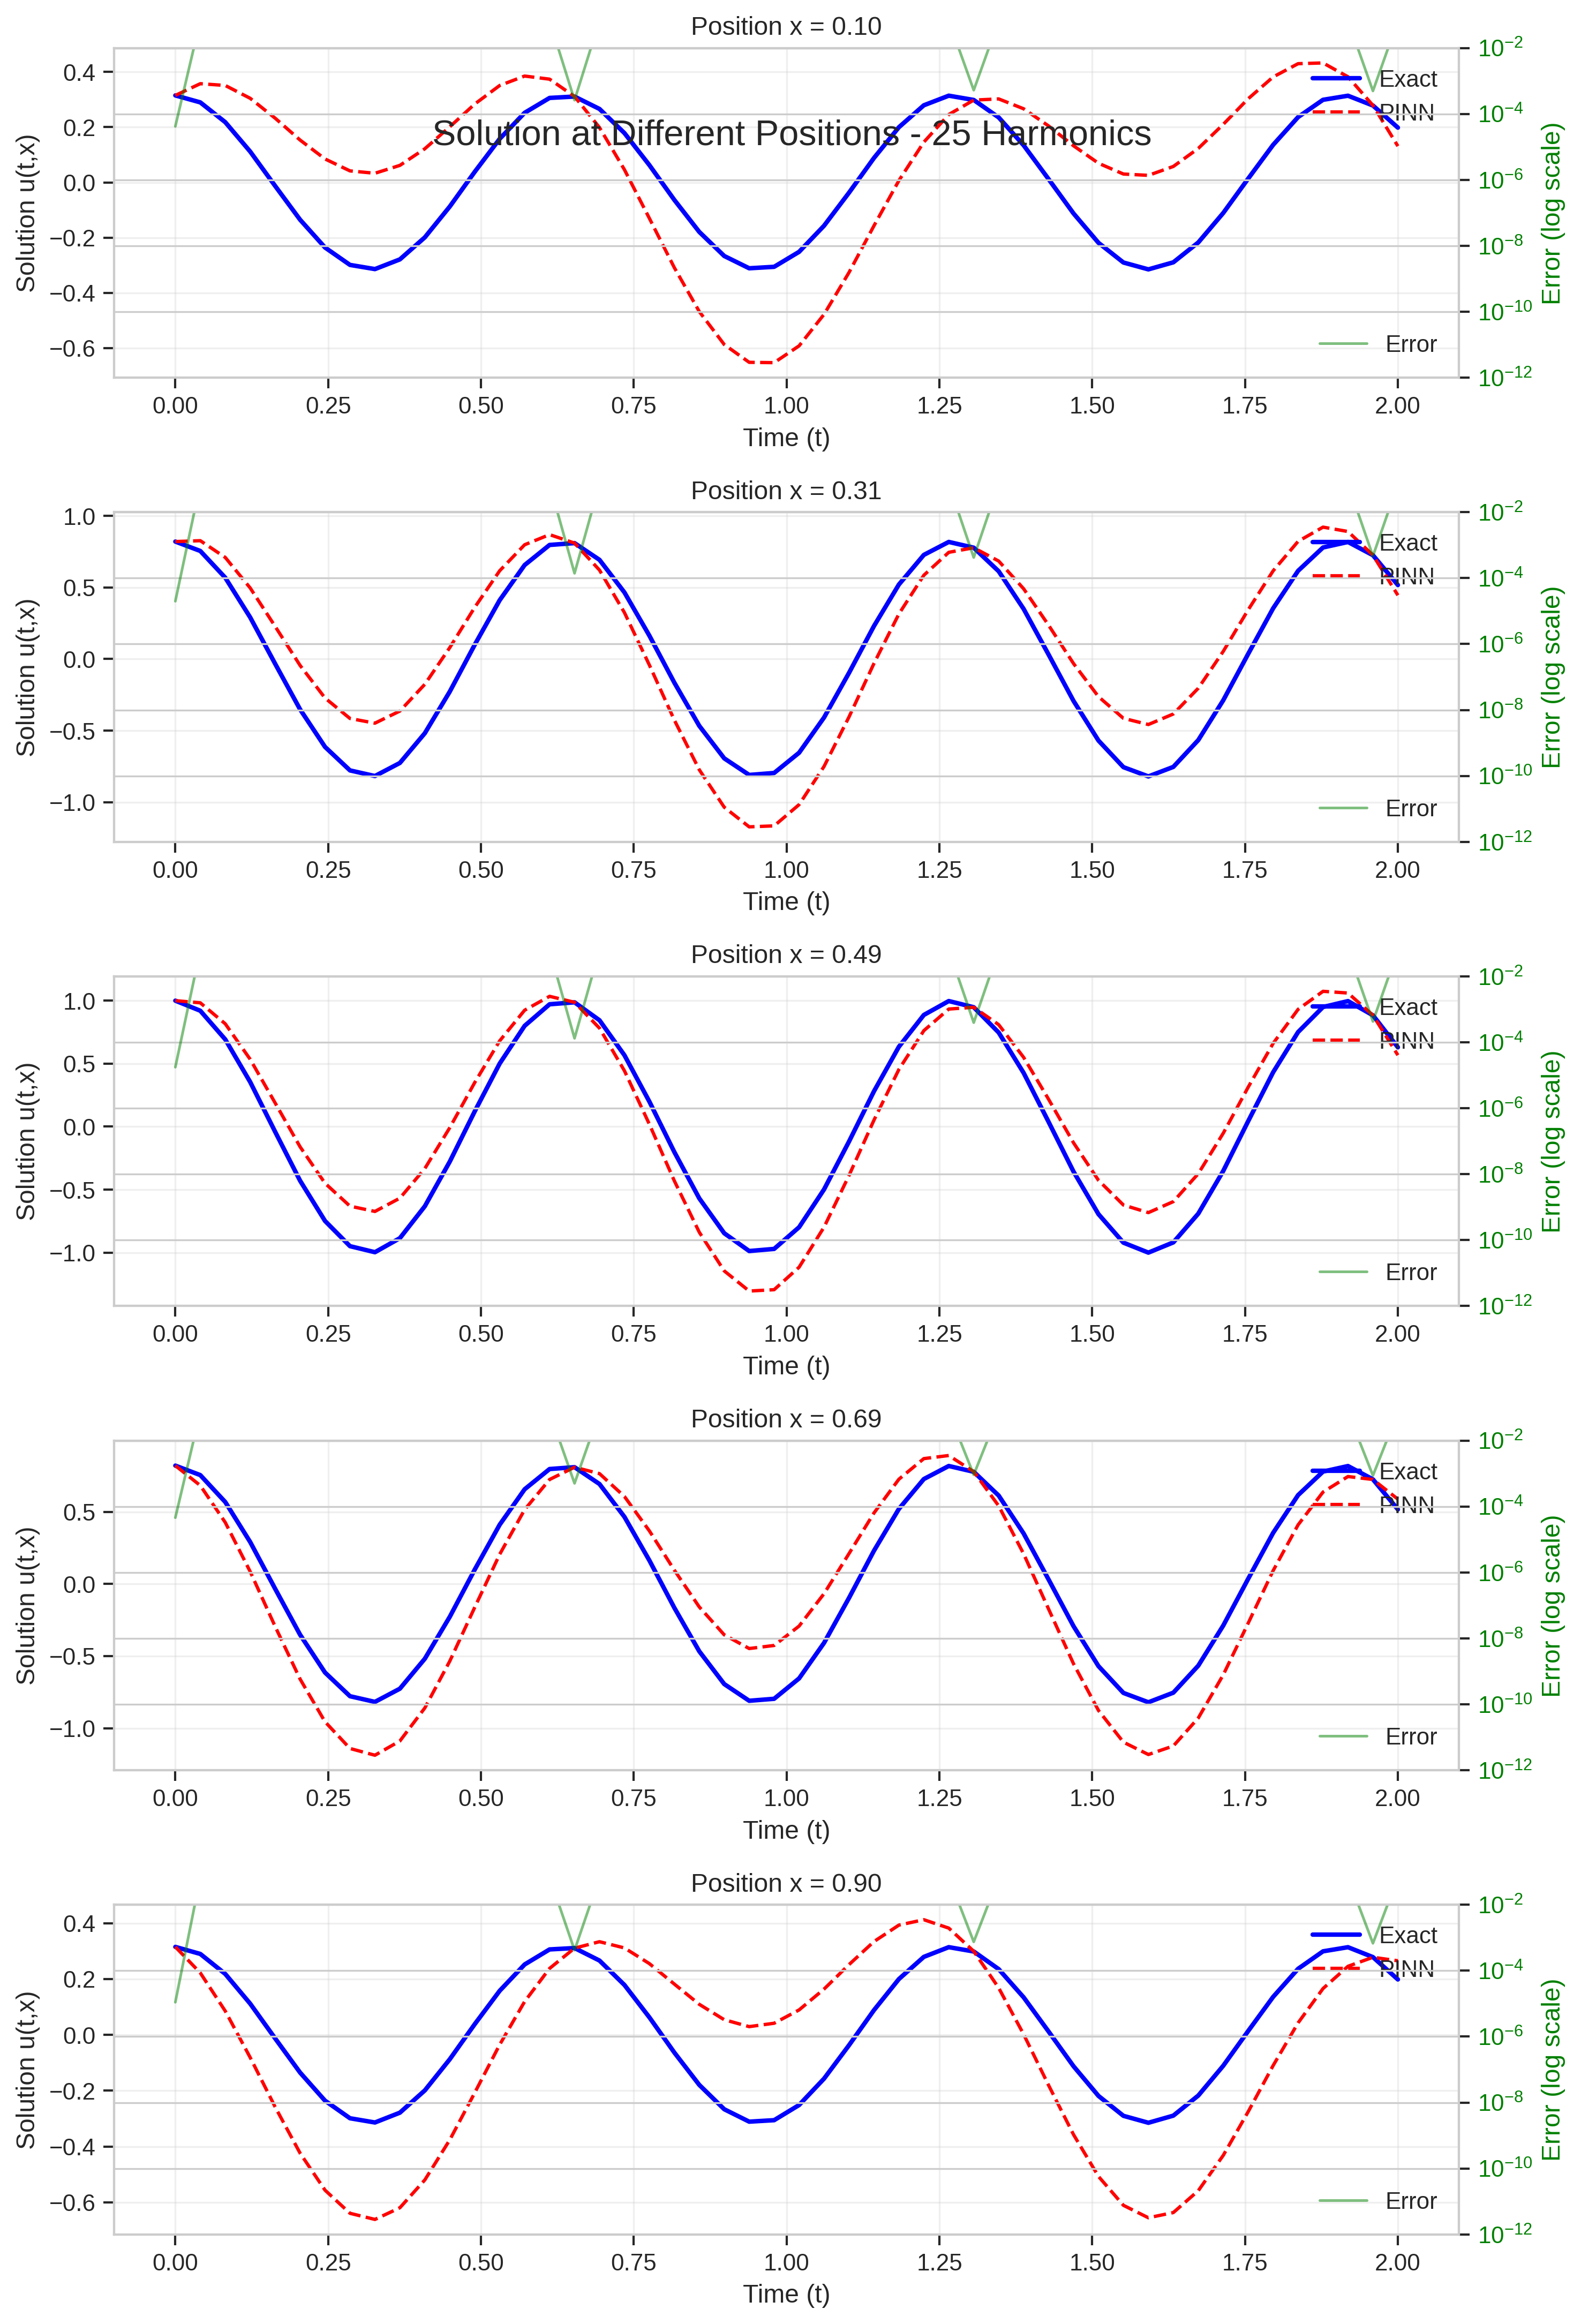
\includegraphics[width=\textwidth]{figures/space_slices_25h.png}
        \caption{25 harmonics}
    \end{subfigure}
    \hfill
    \begin{subfigure}[b]{0.32\textwidth}
        \centering
        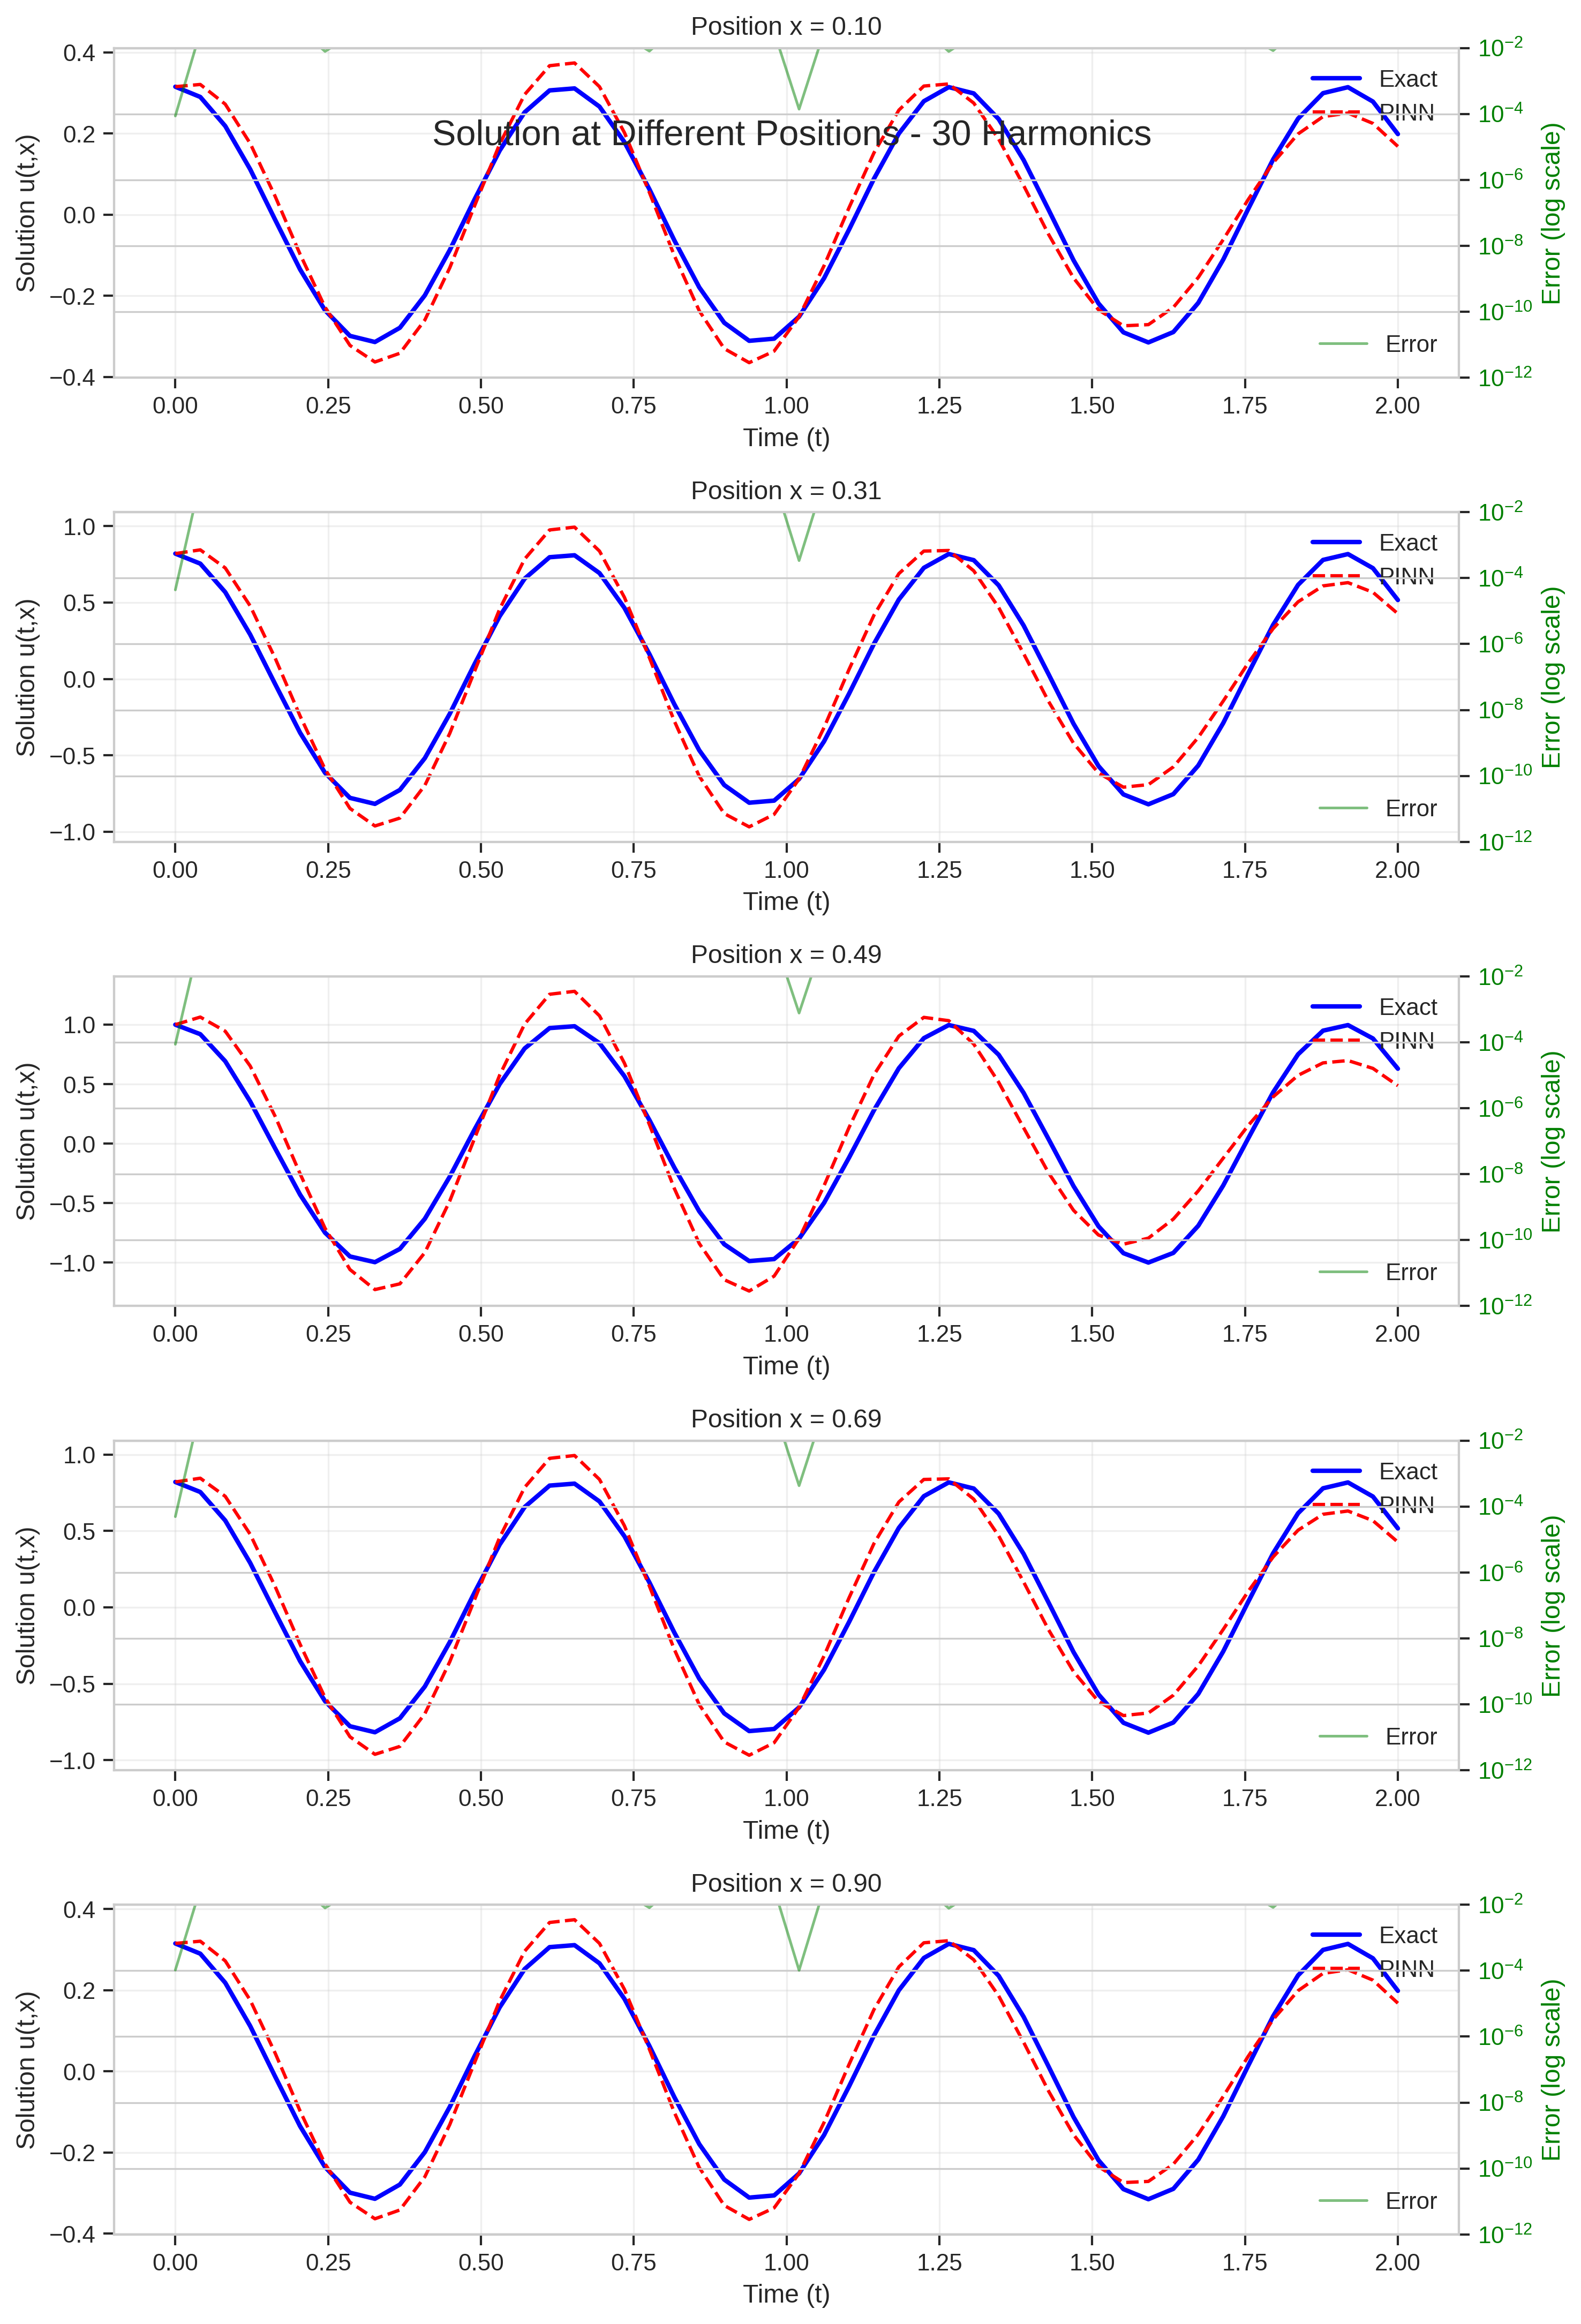
\includegraphics[width=\textwidth]{figures/space_slices_30h.png}
        \caption{30 harmonics}
    \end{subfigure}
    \caption{Spatial solution profiles at fixed time points for mid-range harmonic counts.}
    \label{fig:space_slices_mid}
\end{figure}

\begin{figure}[H]
    \centering
    \begin{subfigure}[b]{0.32\textwidth}
        \centering
        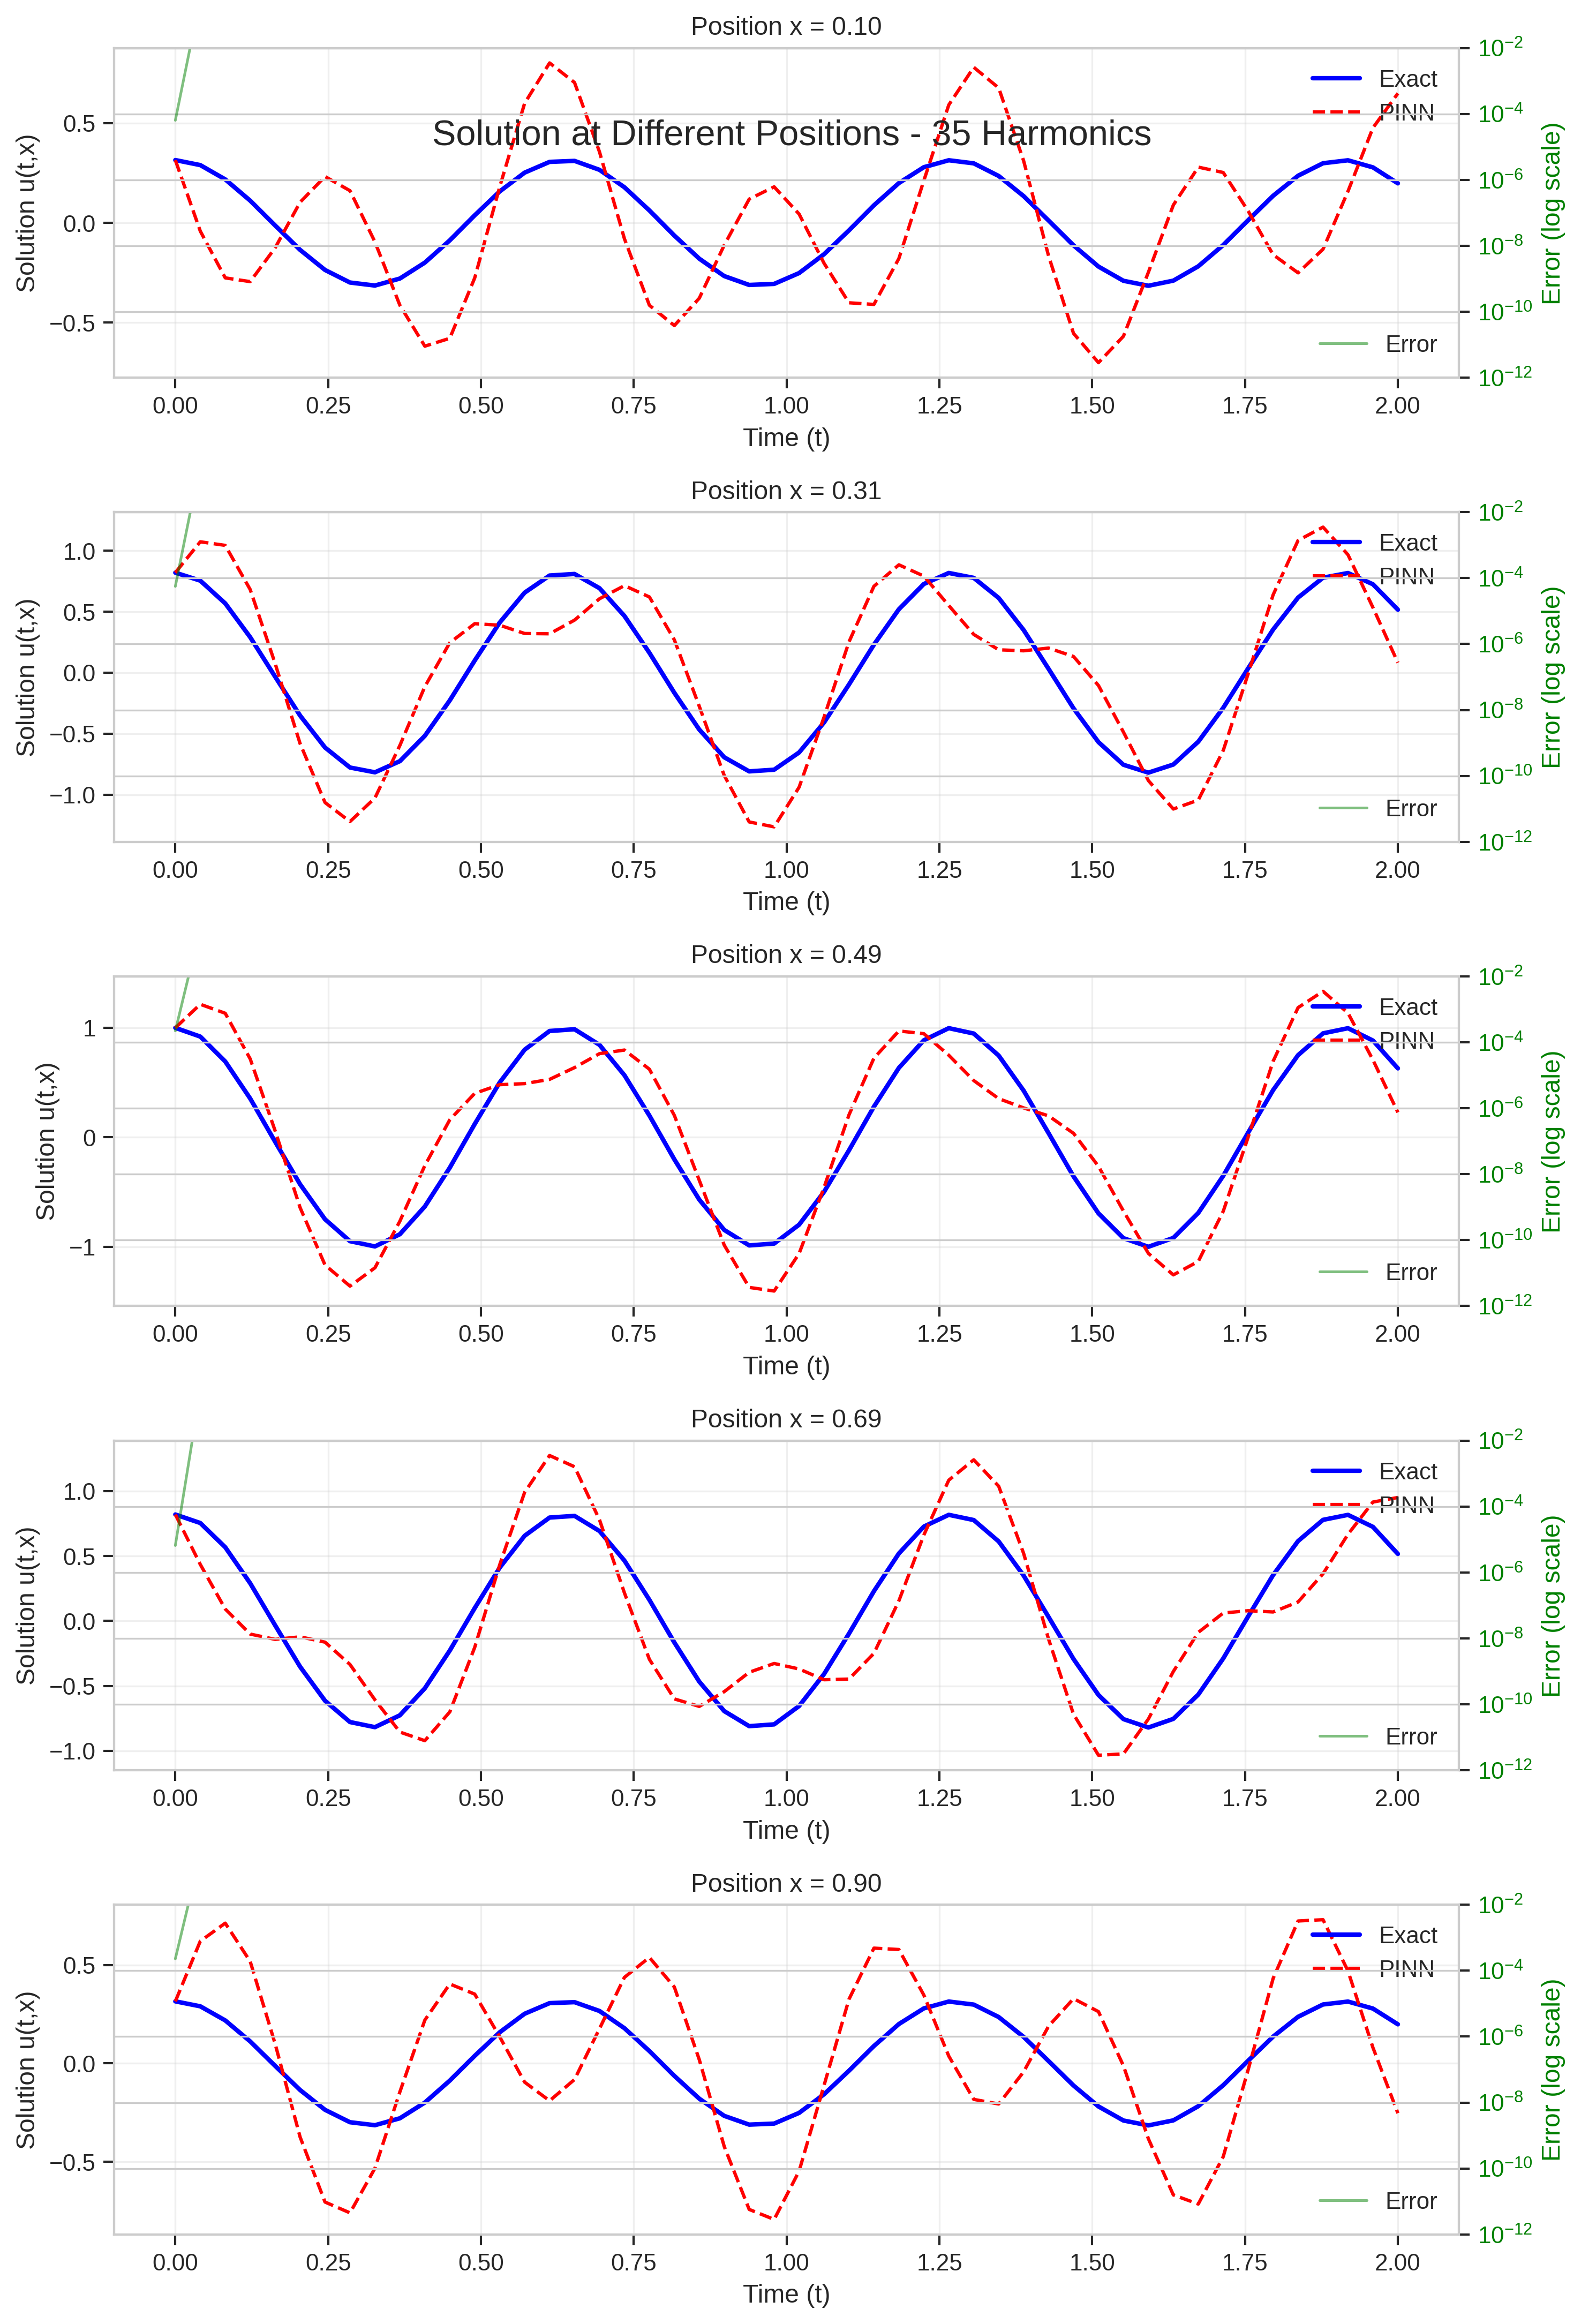
\includegraphics[width=\textwidth]{figures/space_slices_35h.png}
        \caption{35 harmonics}
    \end{subfigure}
    \hfill
    \begin{subfigure}[b]{0.32\textwidth}
        \centering
        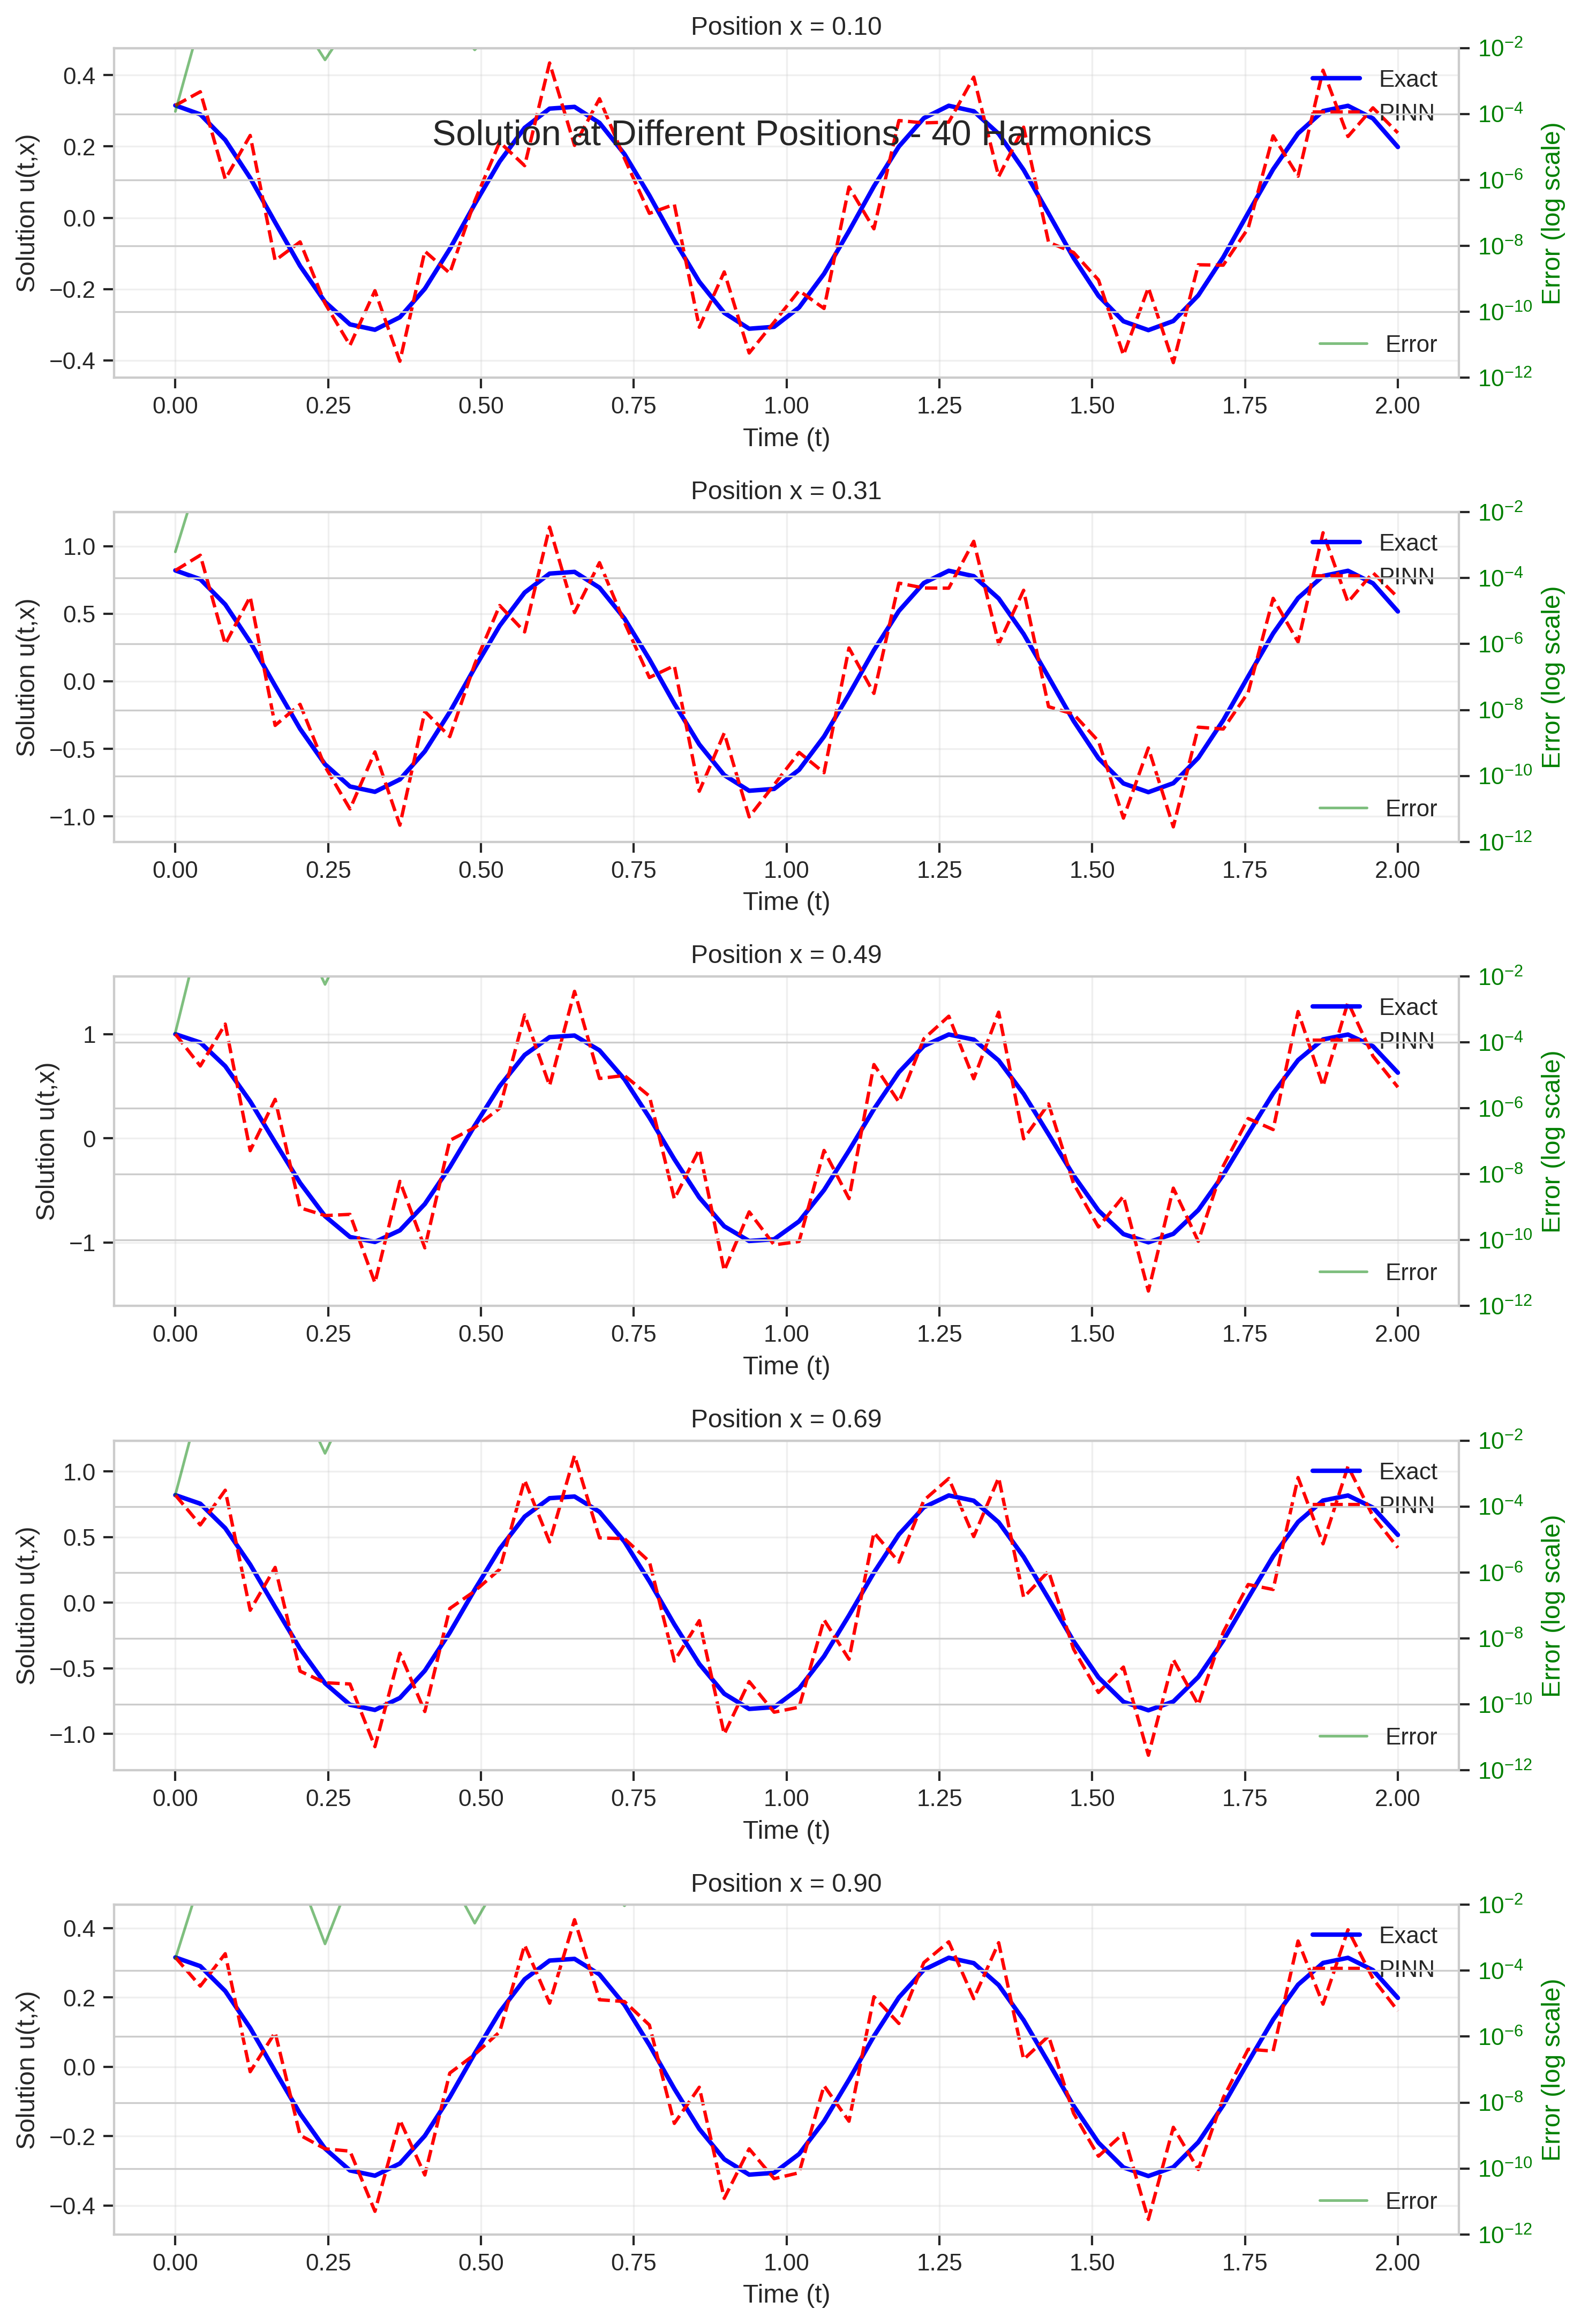
\includegraphics[width=\textwidth]{figures/space_slices_40h.png}
        \caption{40 harmonics}
    \end{subfigure}
    \hfill
    \begin{subfigure}[b]{0.32\textwidth}
        \centering
        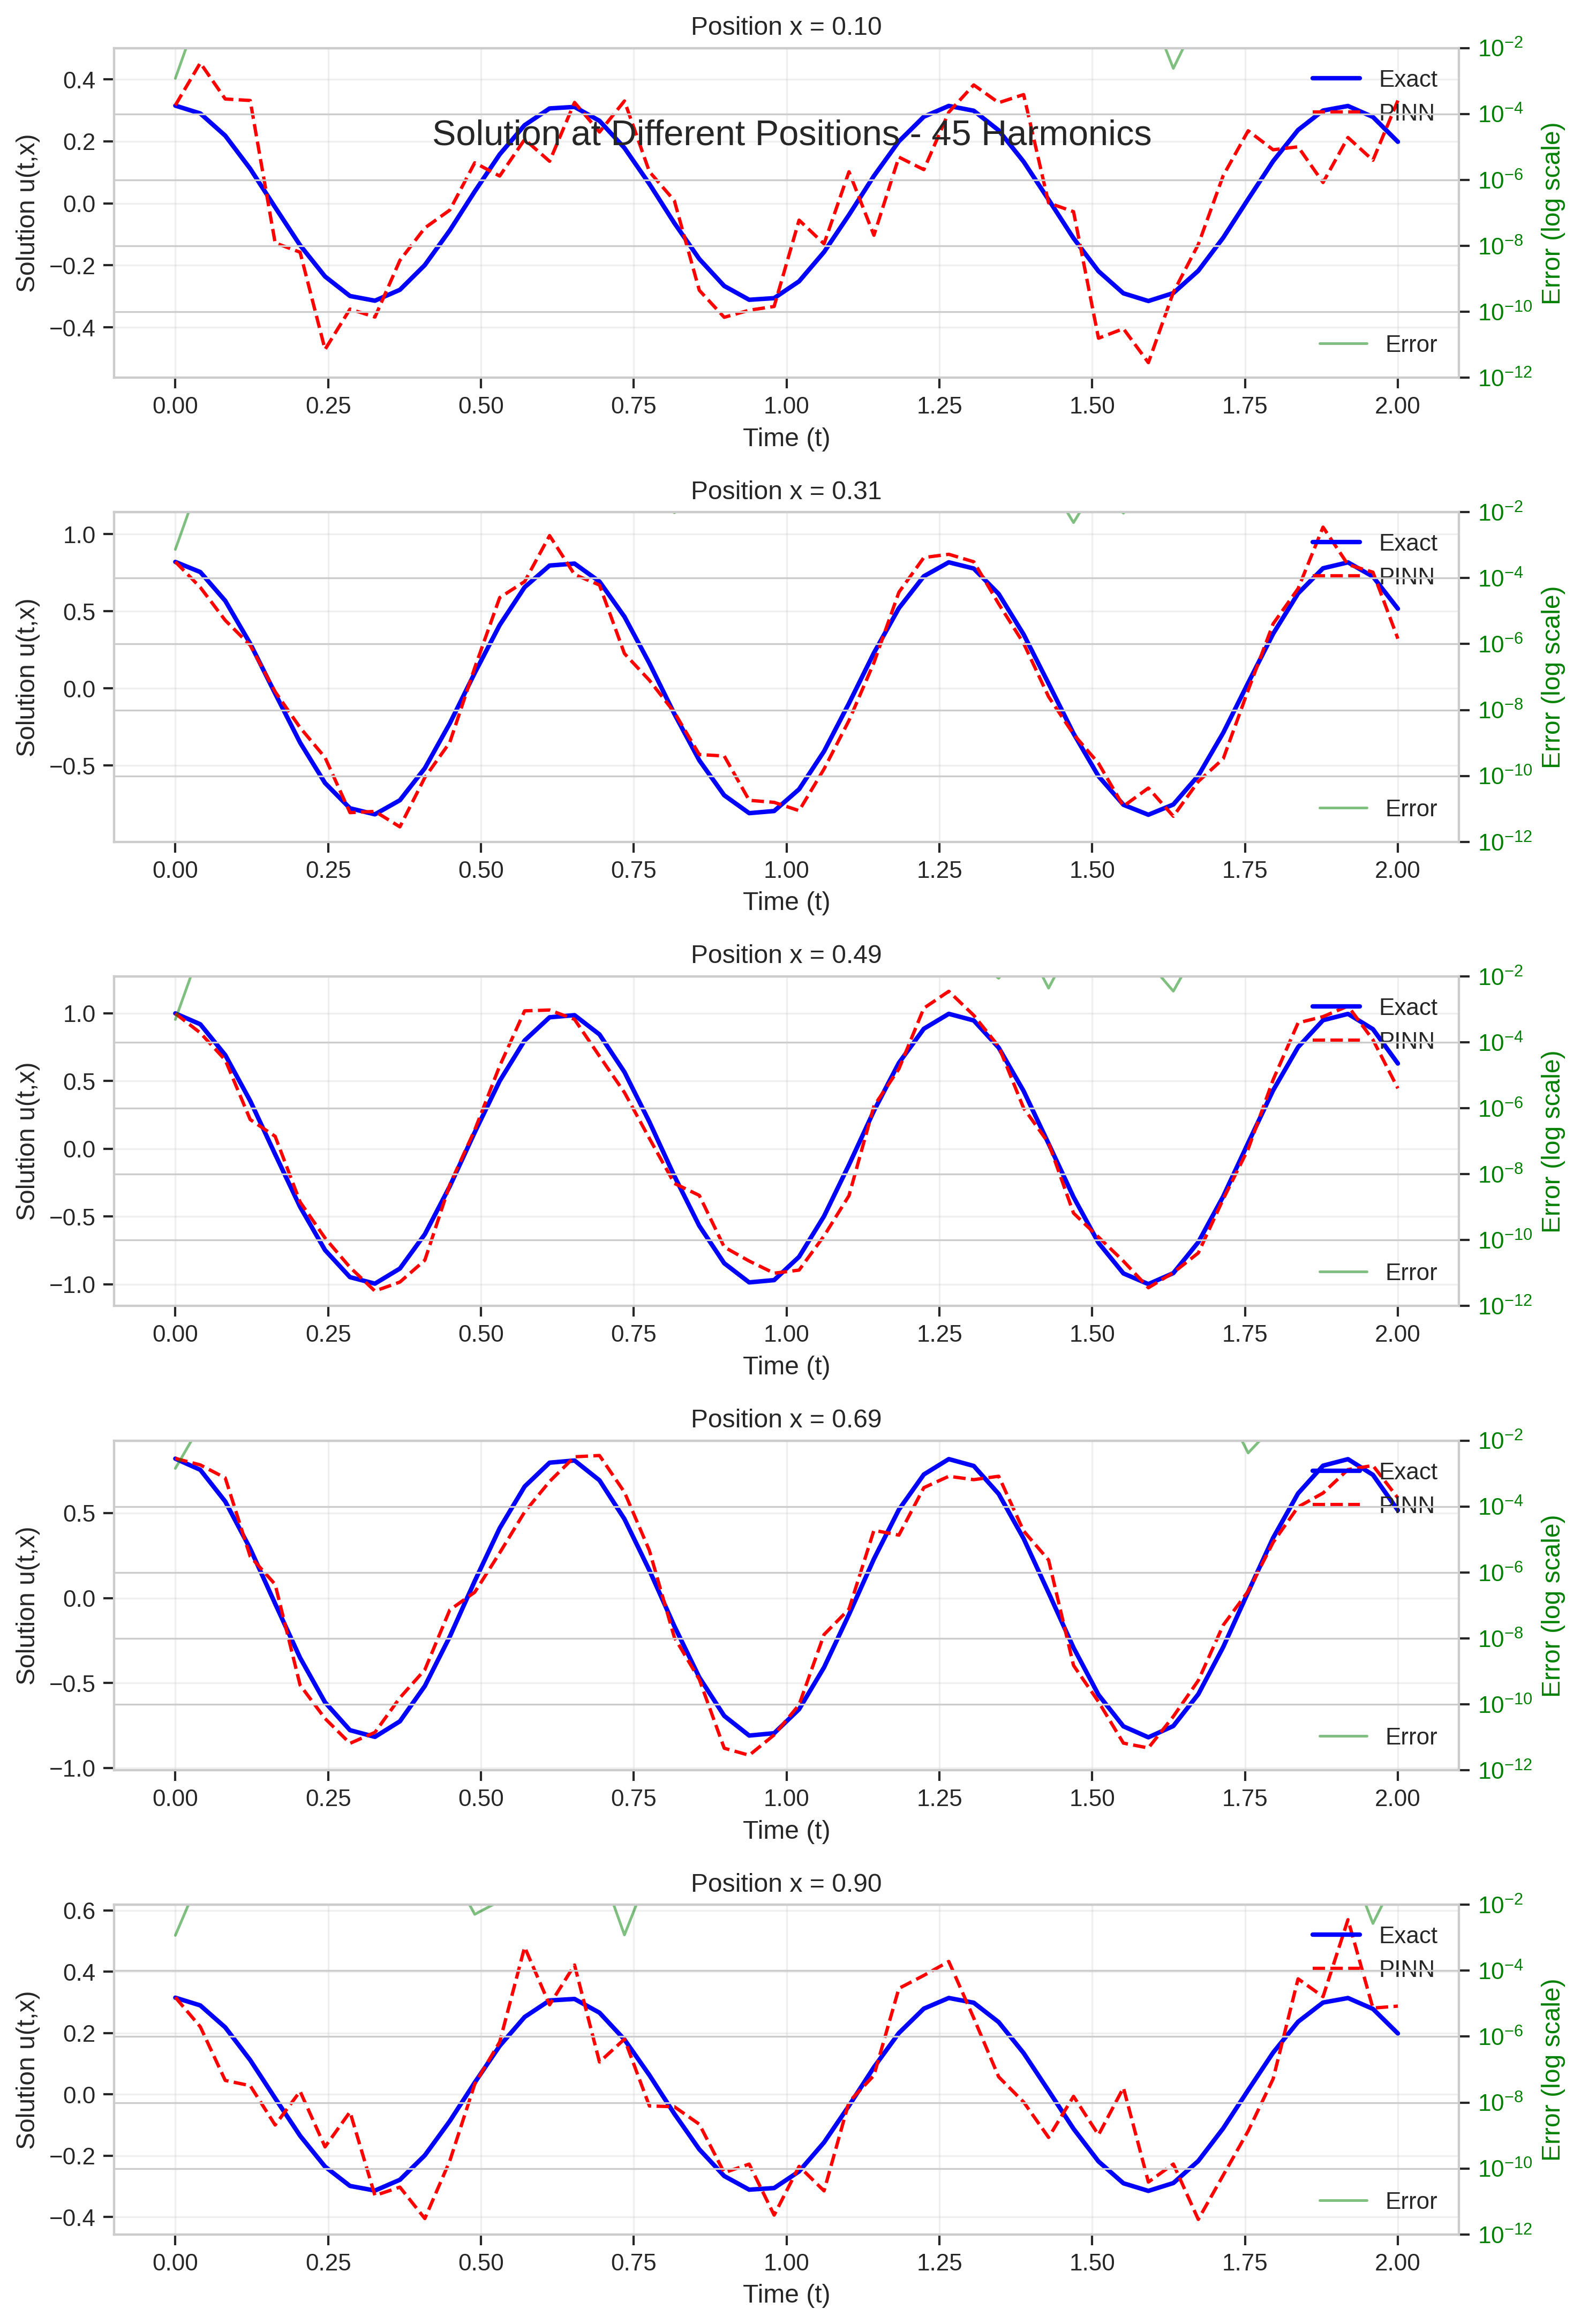
\includegraphics[width=\textwidth]{figures/space_slices_45h.png}
        \caption{45 harmonics}
    \end{subfigure}
    \caption{Spatial profiles for high harmonic configurations demonstrating increasing inaccuracy.}
    \label{fig:space_slices_high}
\end{figure}

\begin{figure}[H]
    \centering
    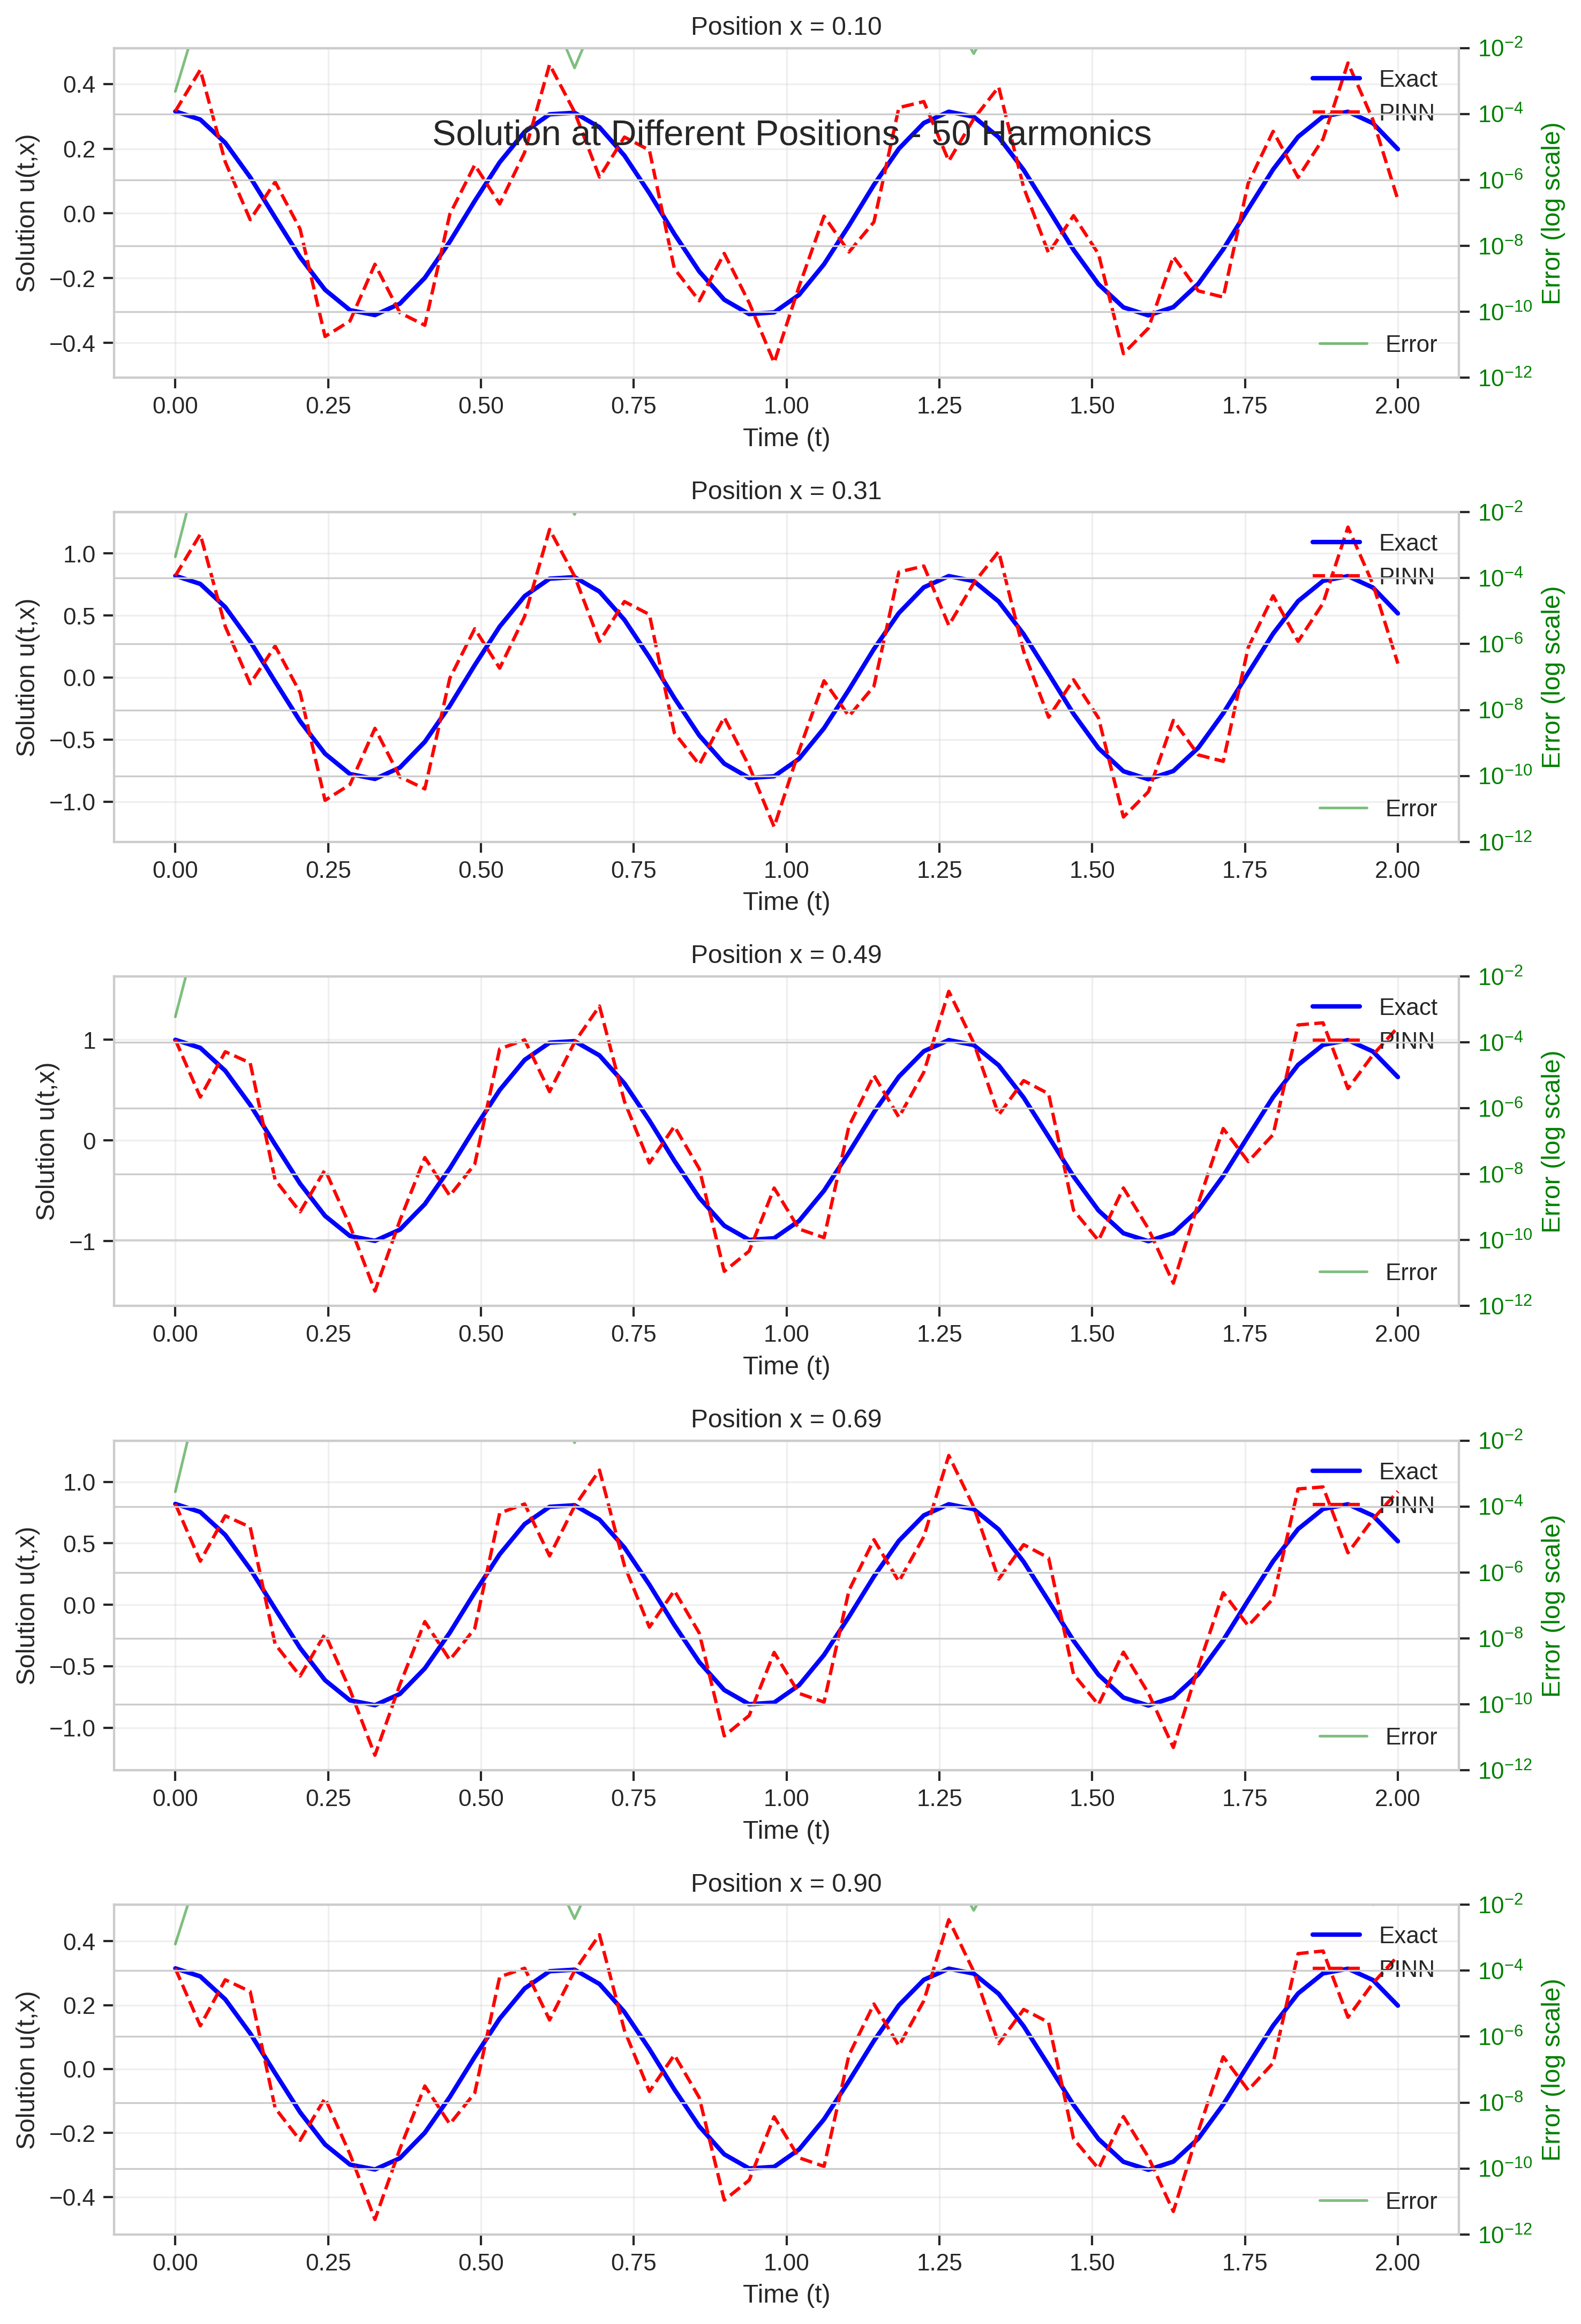
\includegraphics[width=0.6\textwidth]{figures/space_slices_50h.png}
    \caption{Spatial slices for 50 harmonics showing the most severe accuracy degradation.}
    \label{fig:space_slices_50h}
\end{figure}

\subsection{Complete Temporal Slice Analysis}

\begin{figure}[H]
    \centering
    \begin{subfigure}[b]{0.32\textwidth}
        \centering
        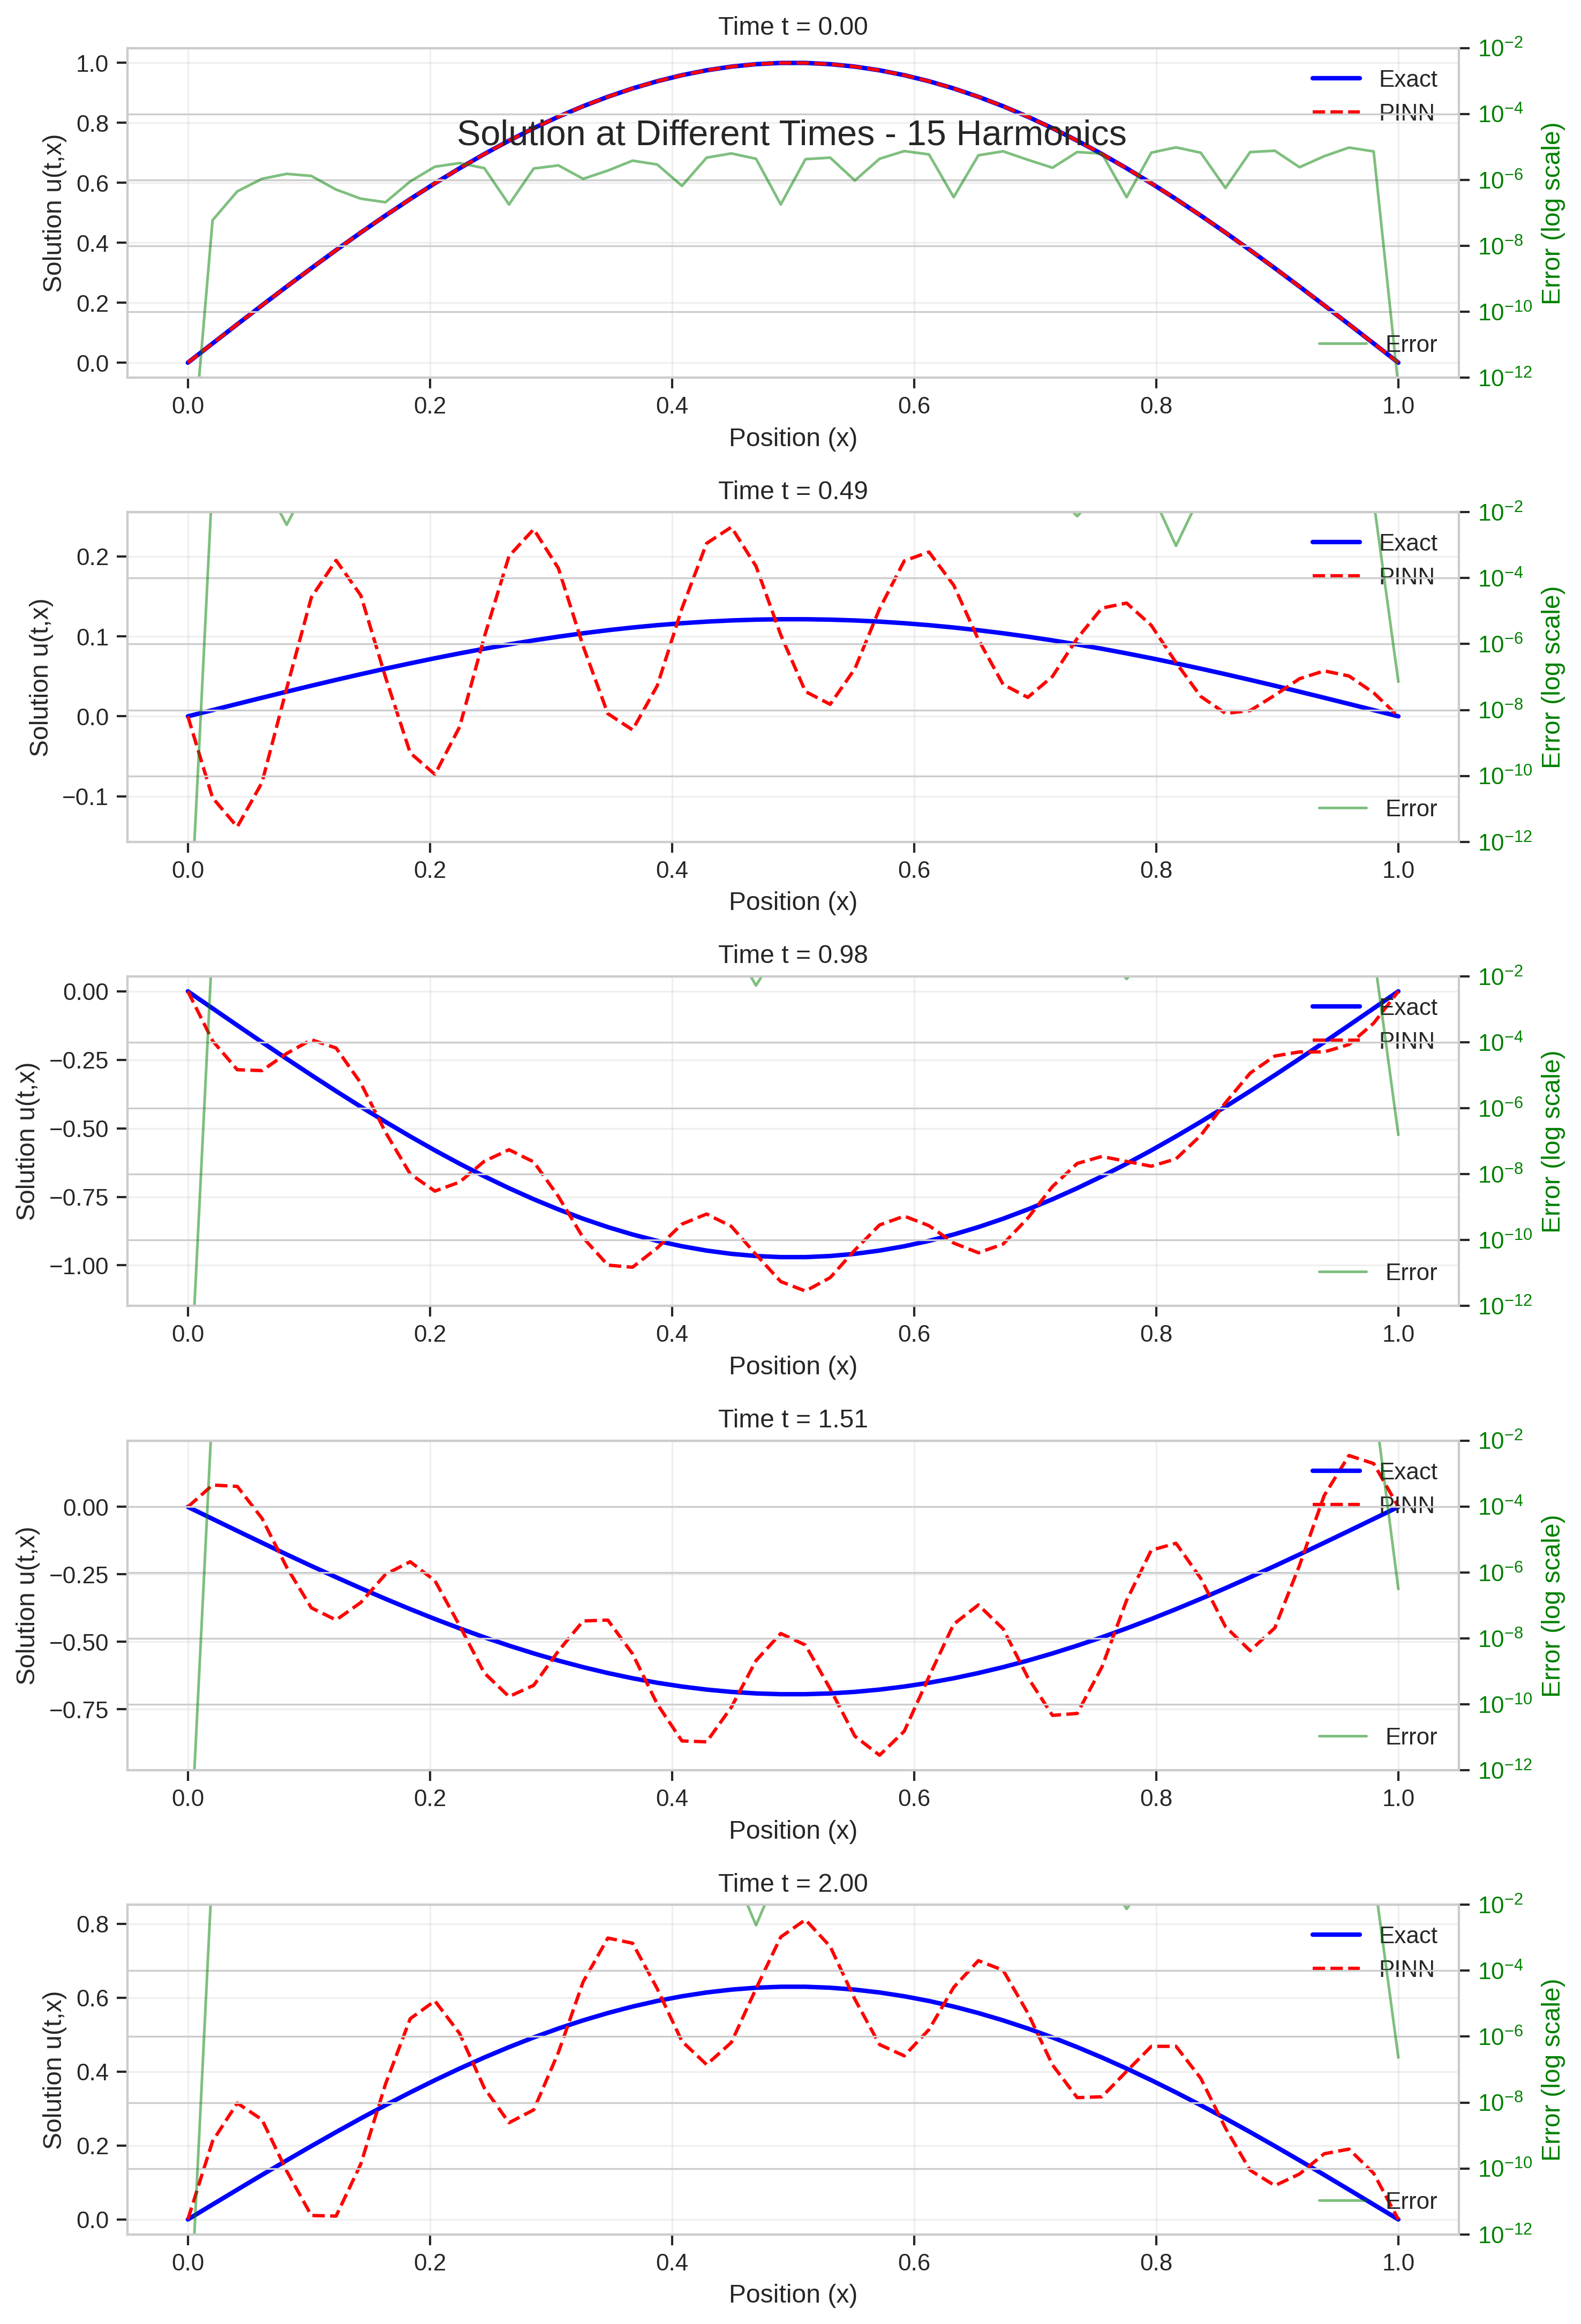
\includegraphics[width=\textwidth]{figures/time_slices_15h.png}
        \caption{15 harmonics}
    \end{subfigure}
    \hfill
    \begin{subfigure}[b]{0.32\textwidth}
        \centering
        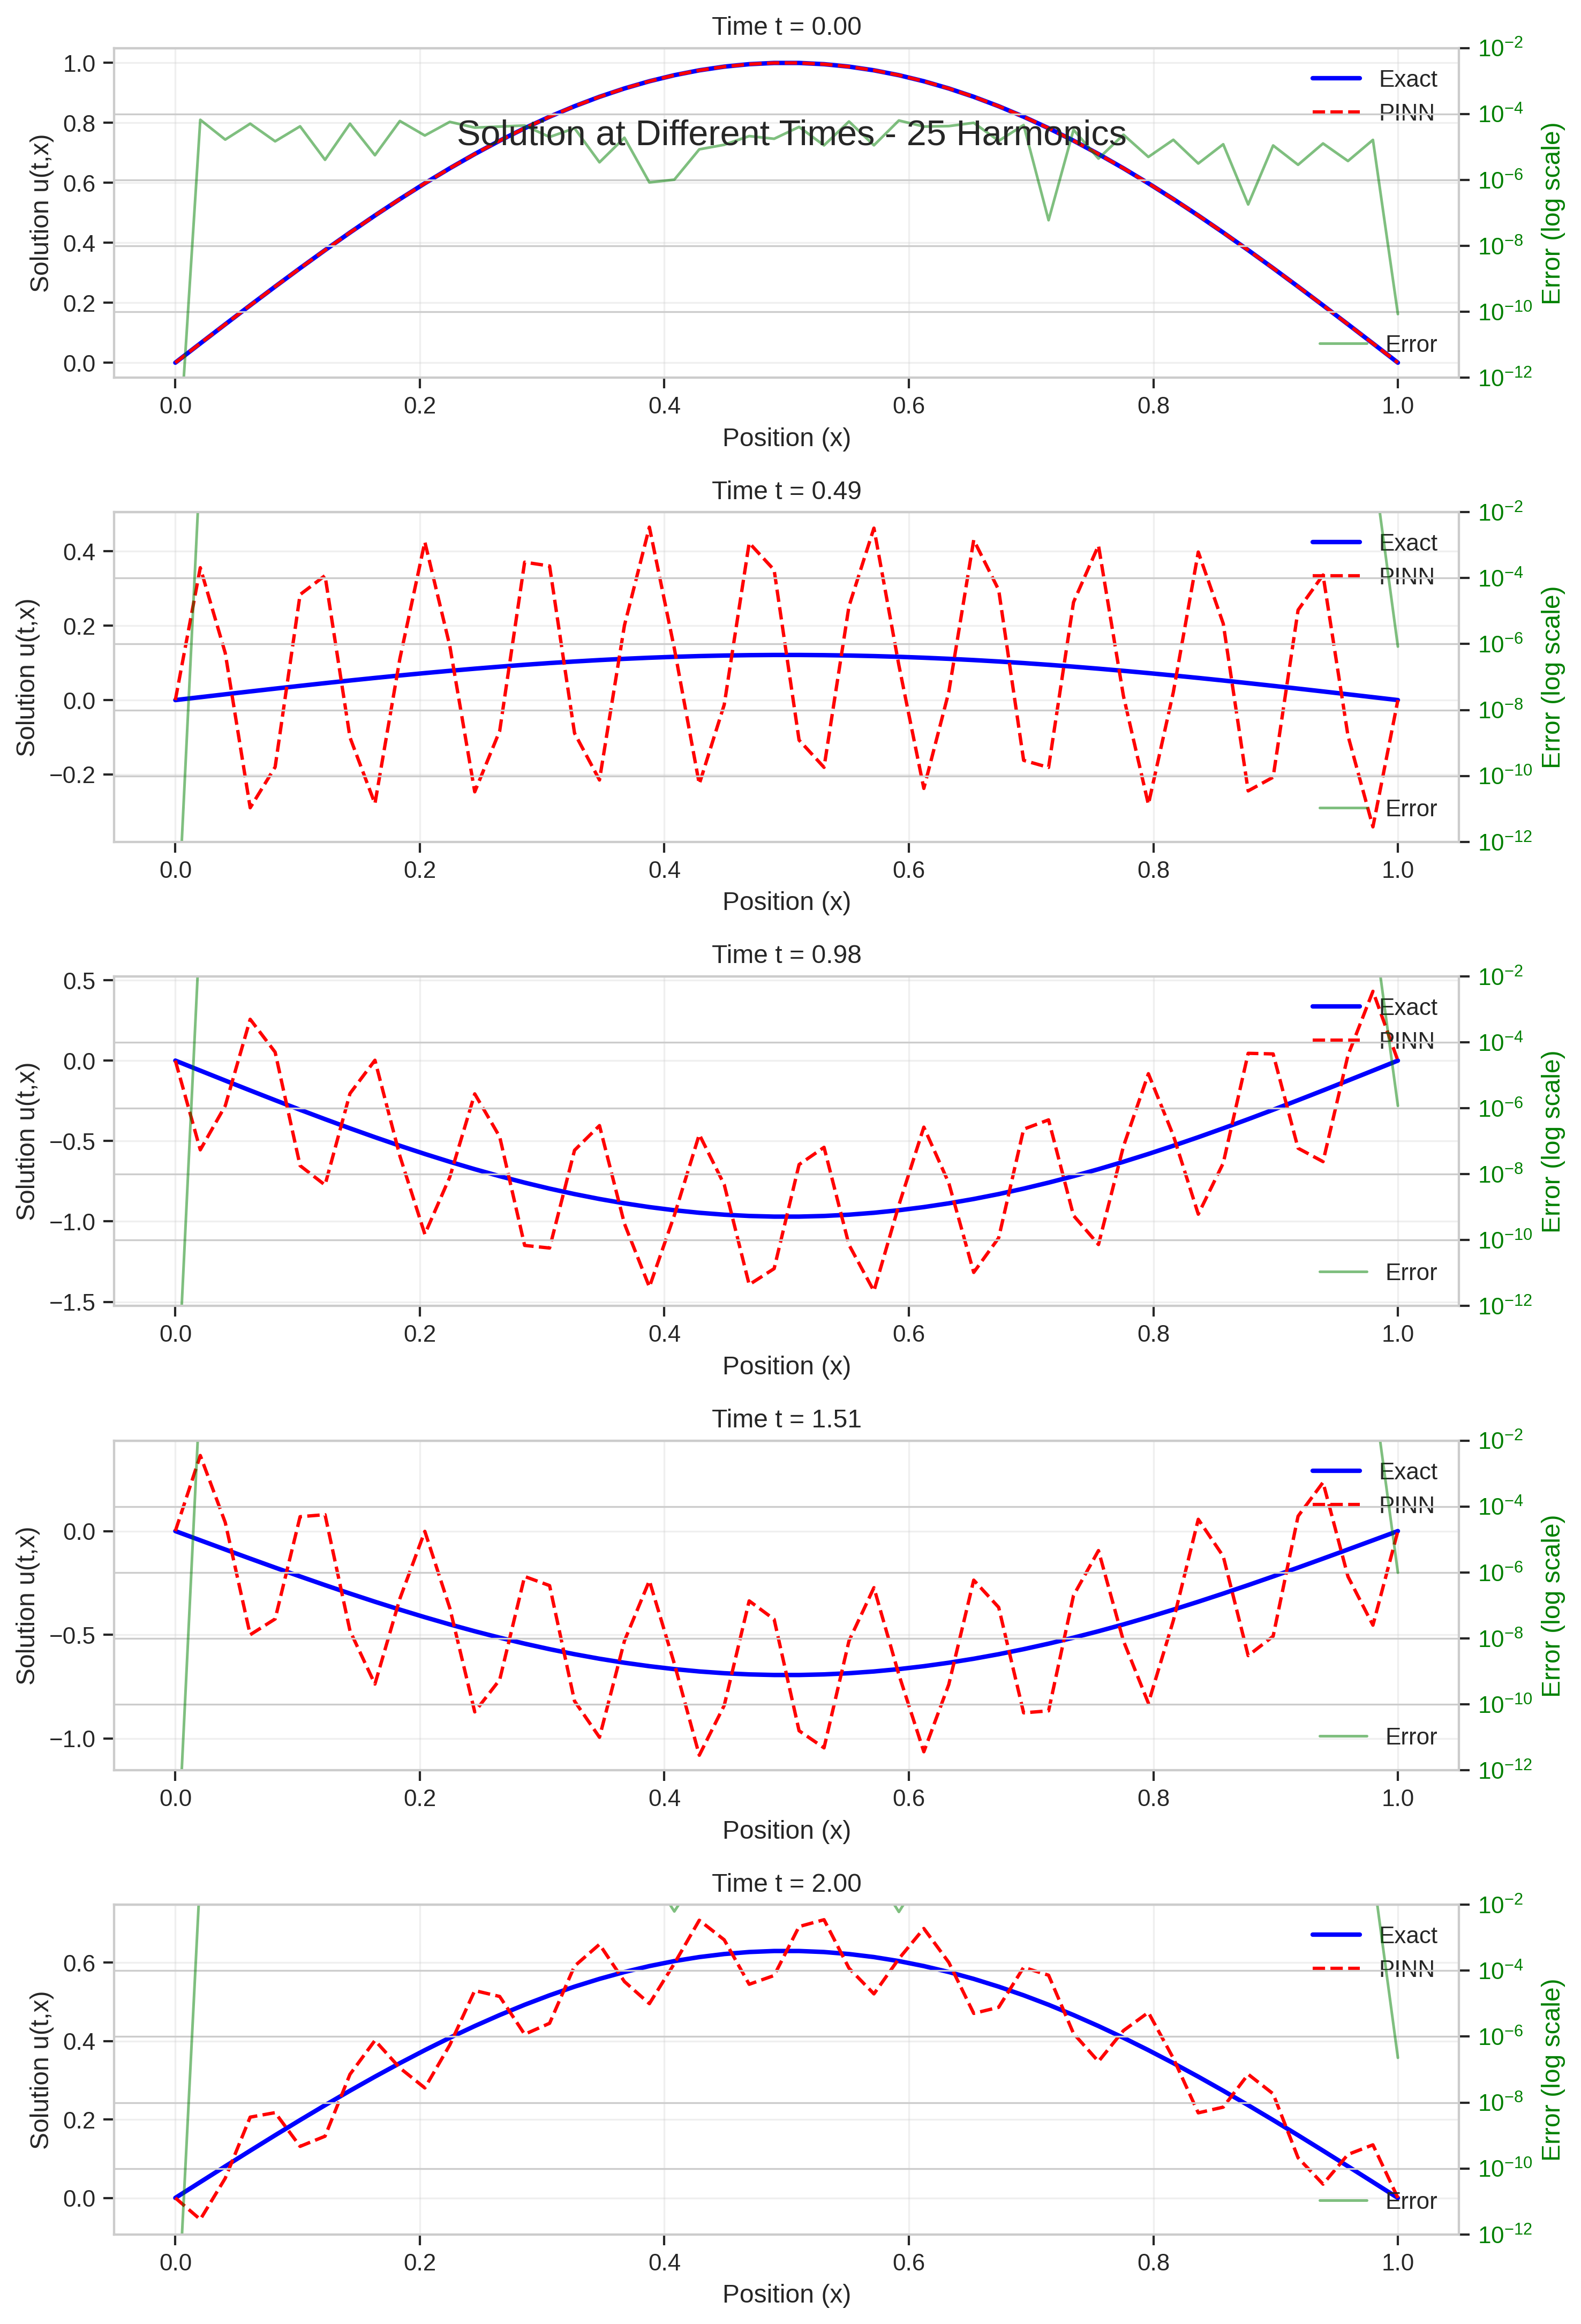
\includegraphics[width=\textwidth]{figures/time_slices_25h.png}
        \caption{25 harmonics}
    \end{subfigure}
    \hfill
    \begin{subfigure}[b]{0.32\textwidth}
        \centering
        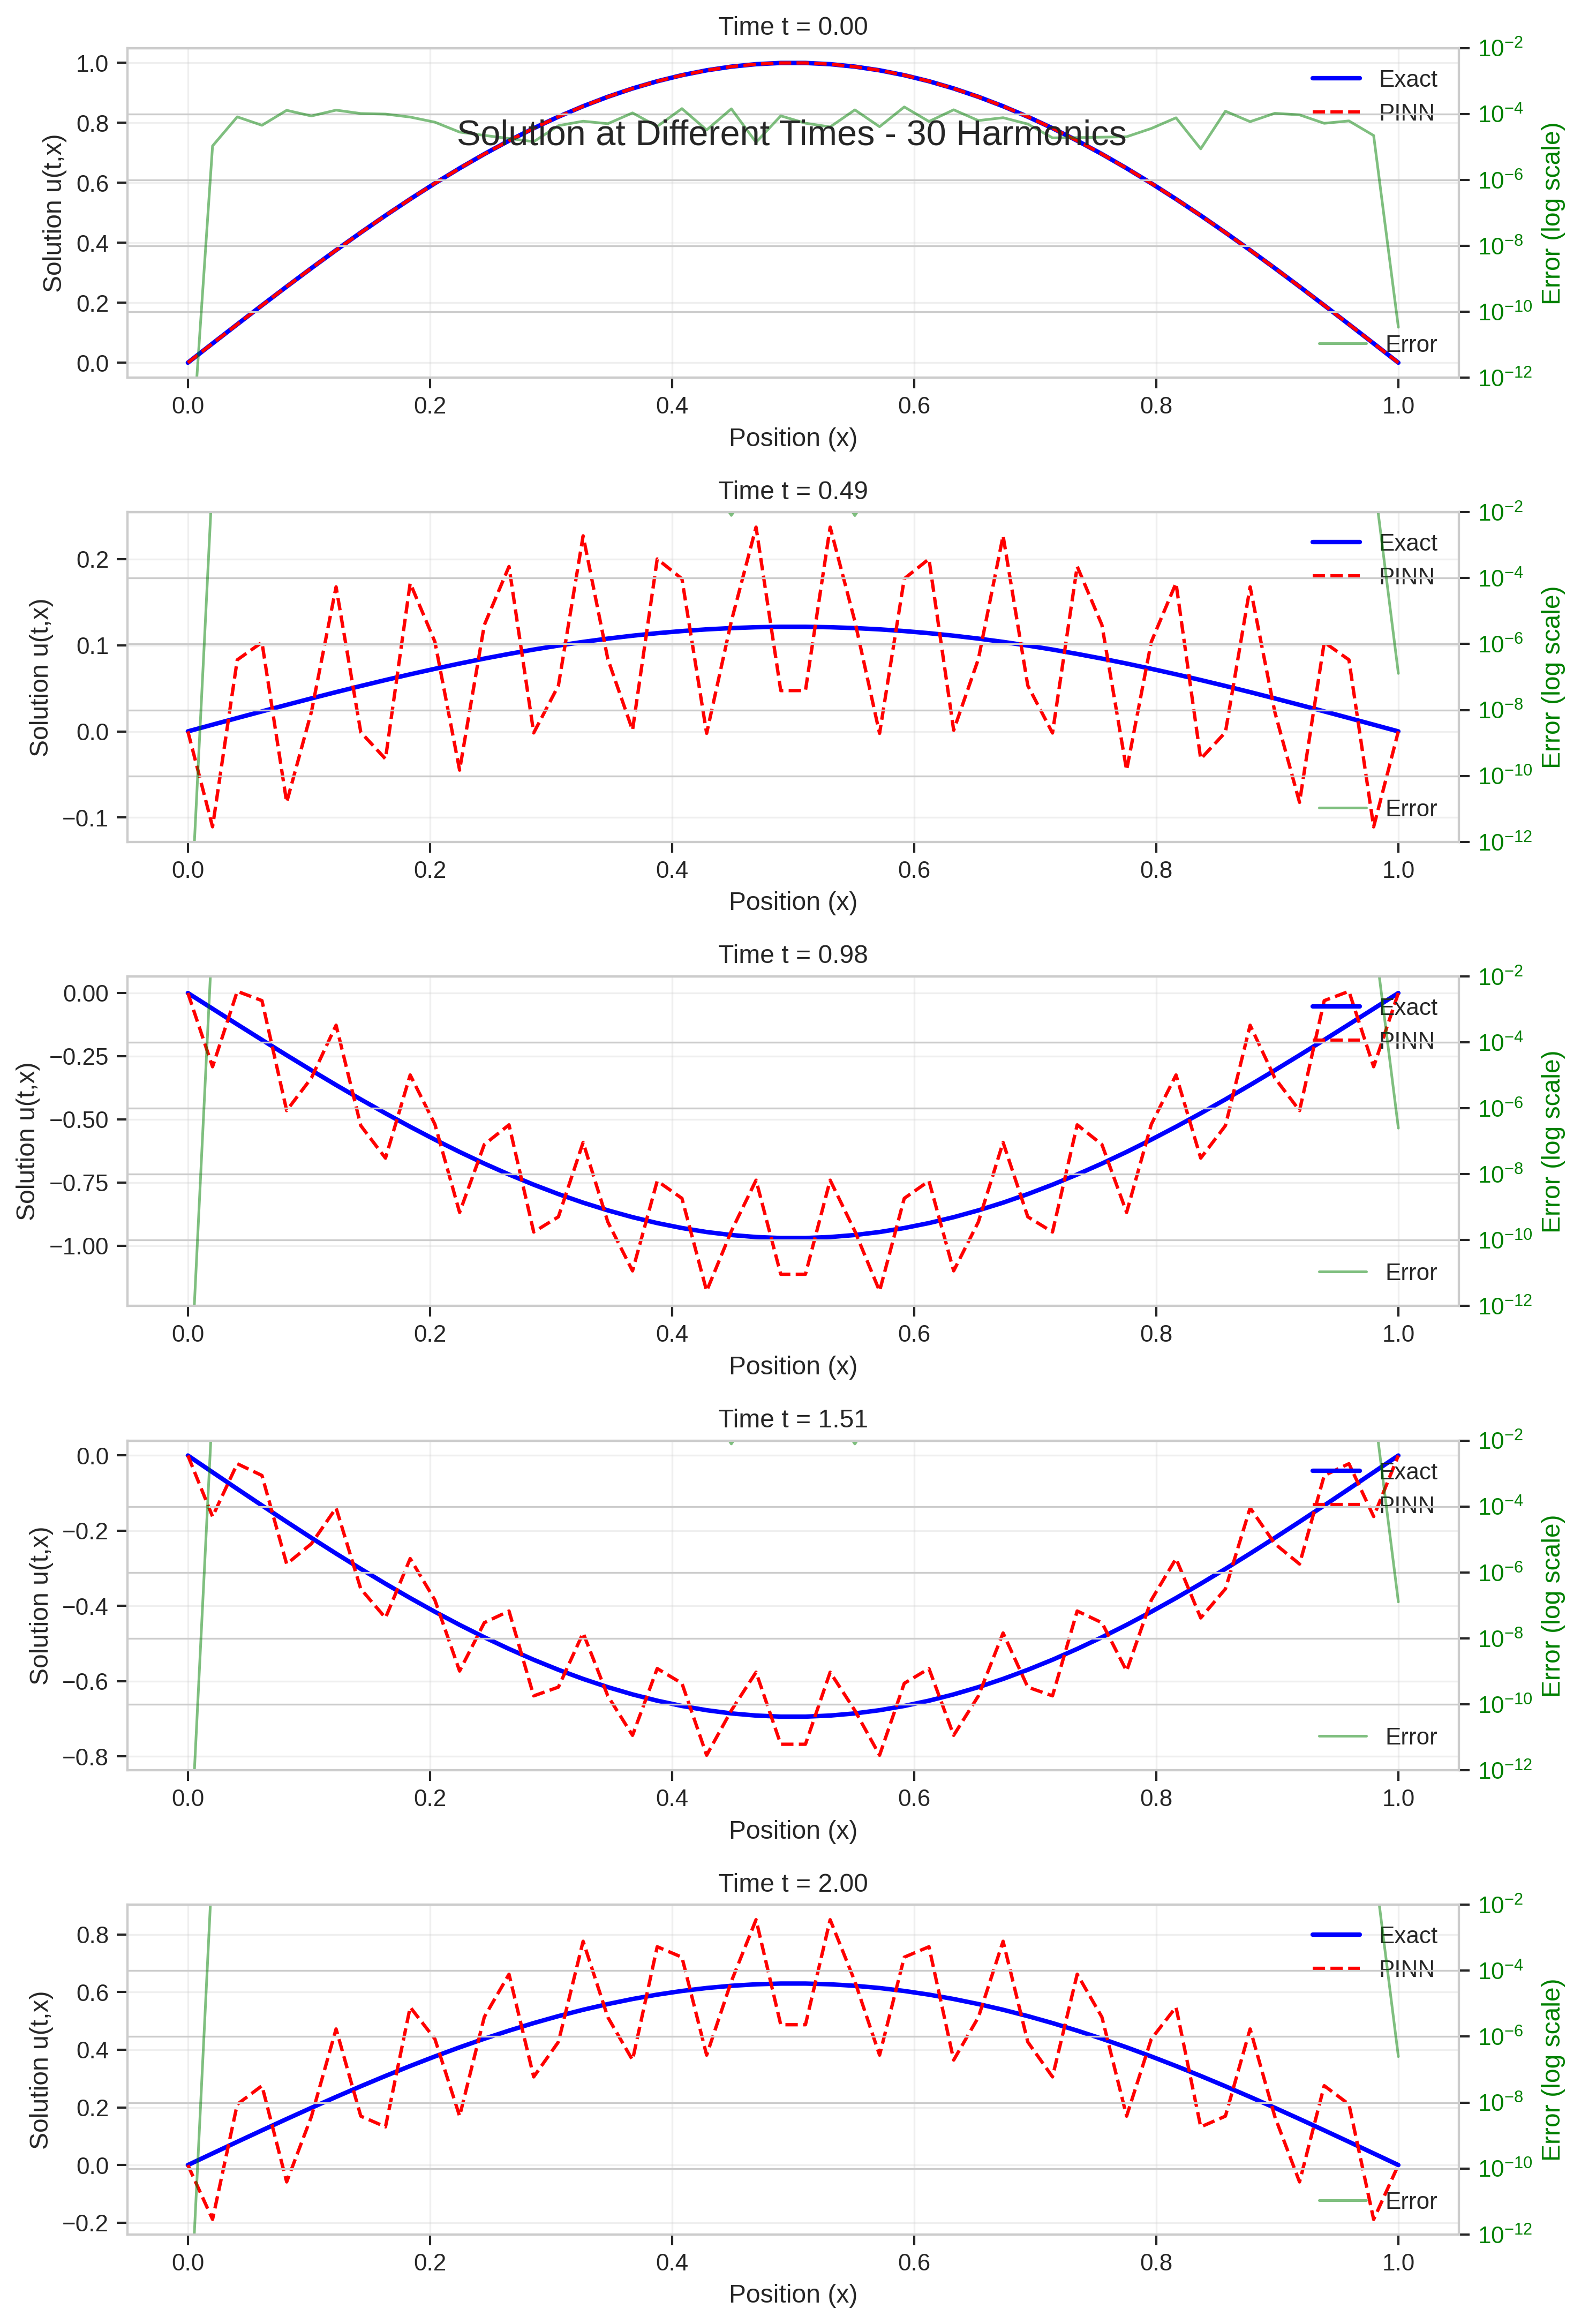
\includegraphics[width=\textwidth]{figures/time_slices_30h.png}
        \caption{30 harmonics}
    \end{subfigure}
    \caption{Temporal evolution at fixed spatial locations for mid-range configurations.}
    \label{fig:time_slices_mid}
\end{figure}

\begin{figure}[H]
    \centering
    \begin{subfigure}[b]{0.32\textwidth}
        \centering
        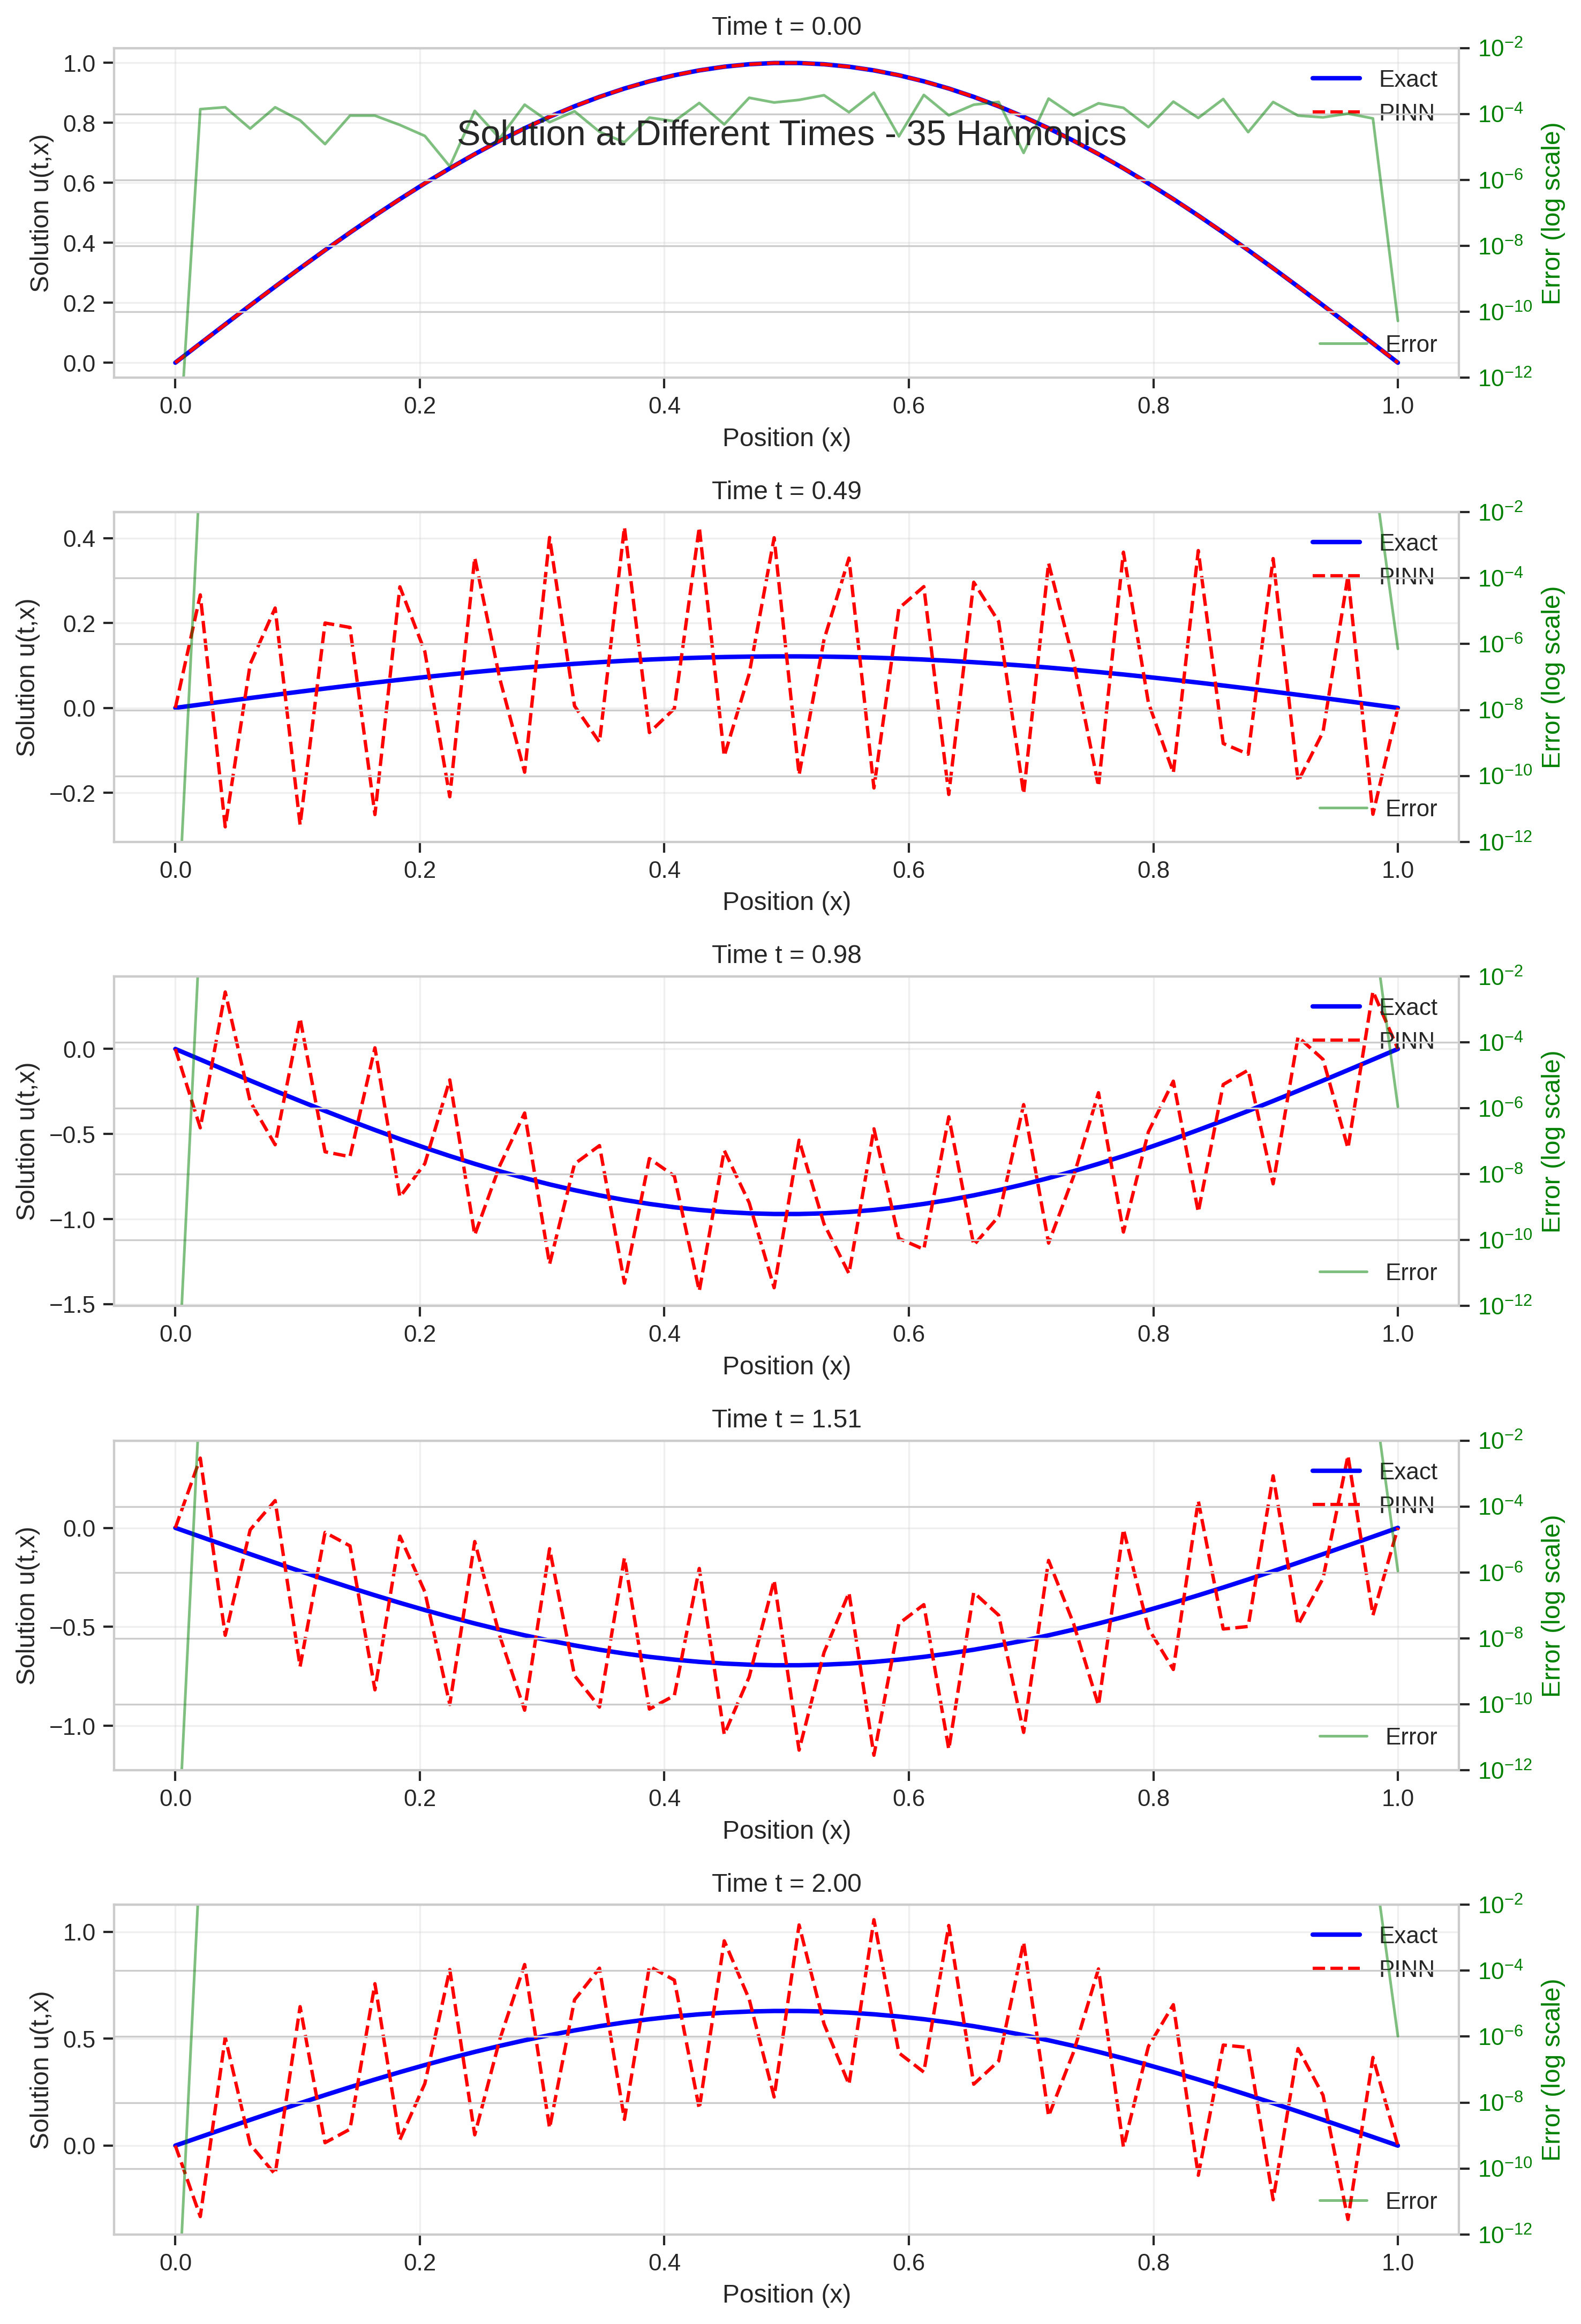
\includegraphics[width=\textwidth]{figures/time_slices_35h.png}
        \caption{35 harmonics}
    \end{subfigure}
    \hfill
    \begin{subfigure}[b]{0.32\textwidth}
        \centering
        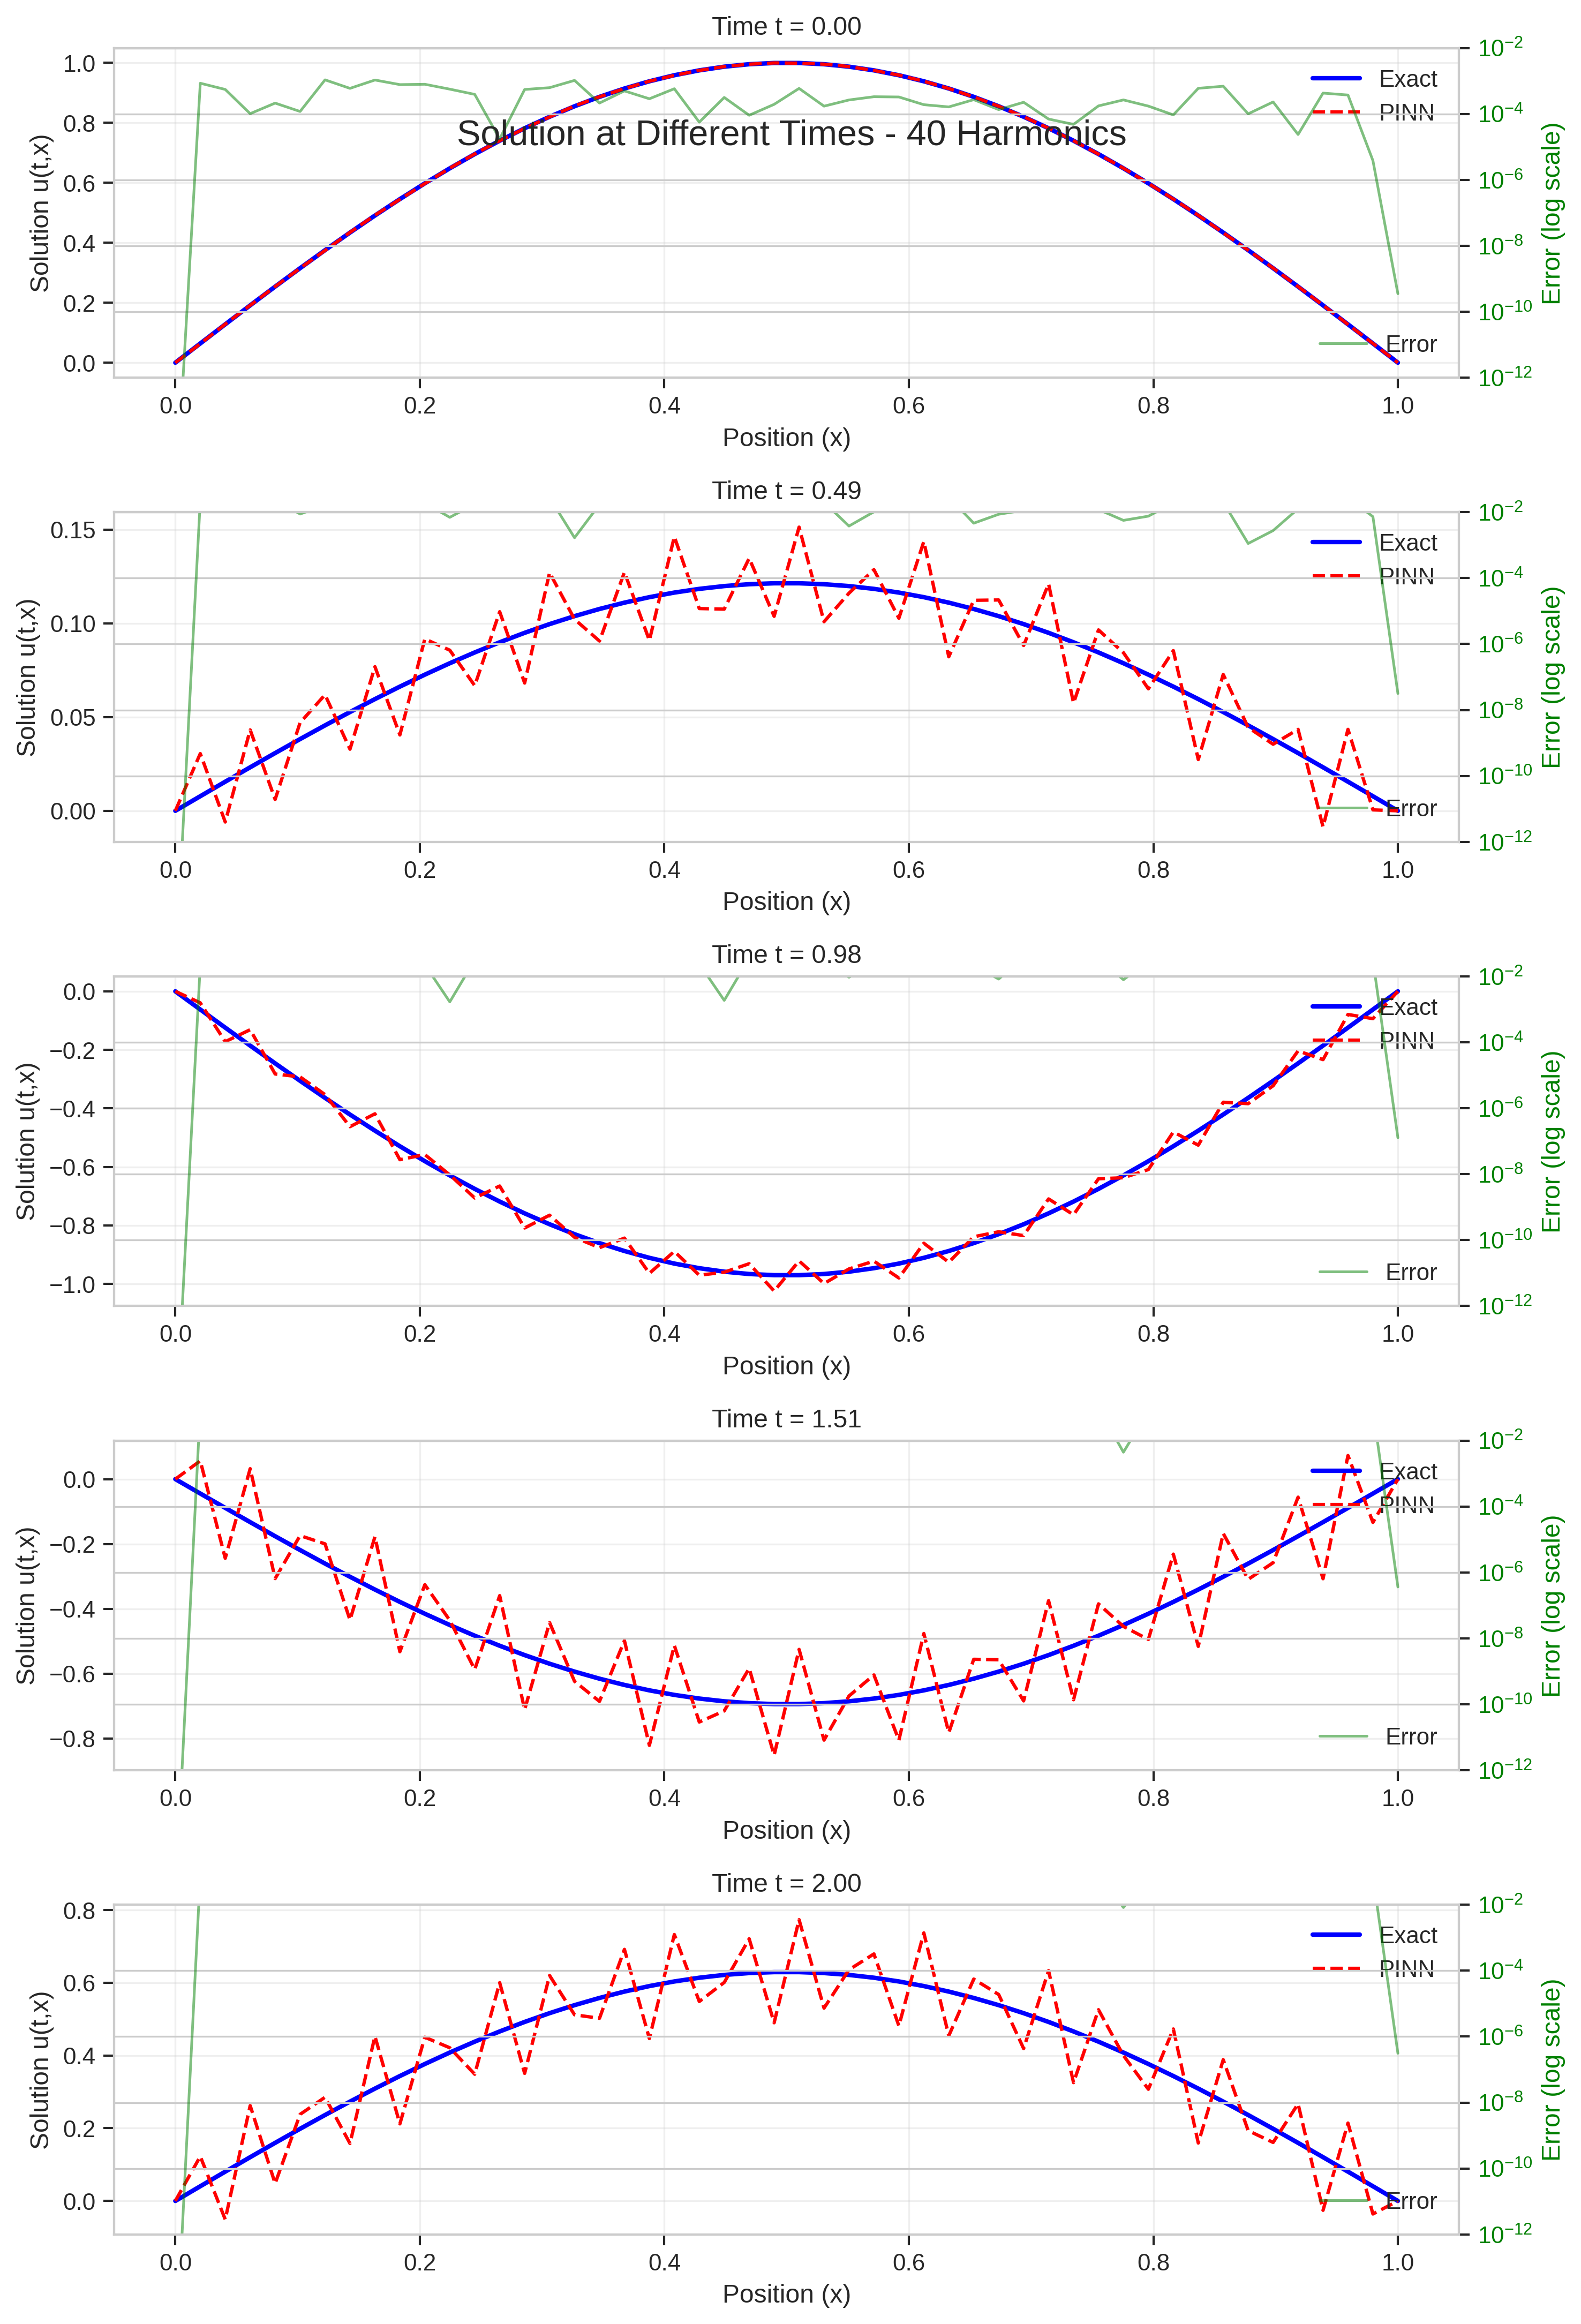
\includegraphics[width=\textwidth]{figures/time_slices_40h.png}
        \caption{40 harmonics}
    \end{subfigure}
    \hfill
    \begin{subfigure}[b]{0.32\textwidth}
        \centering
        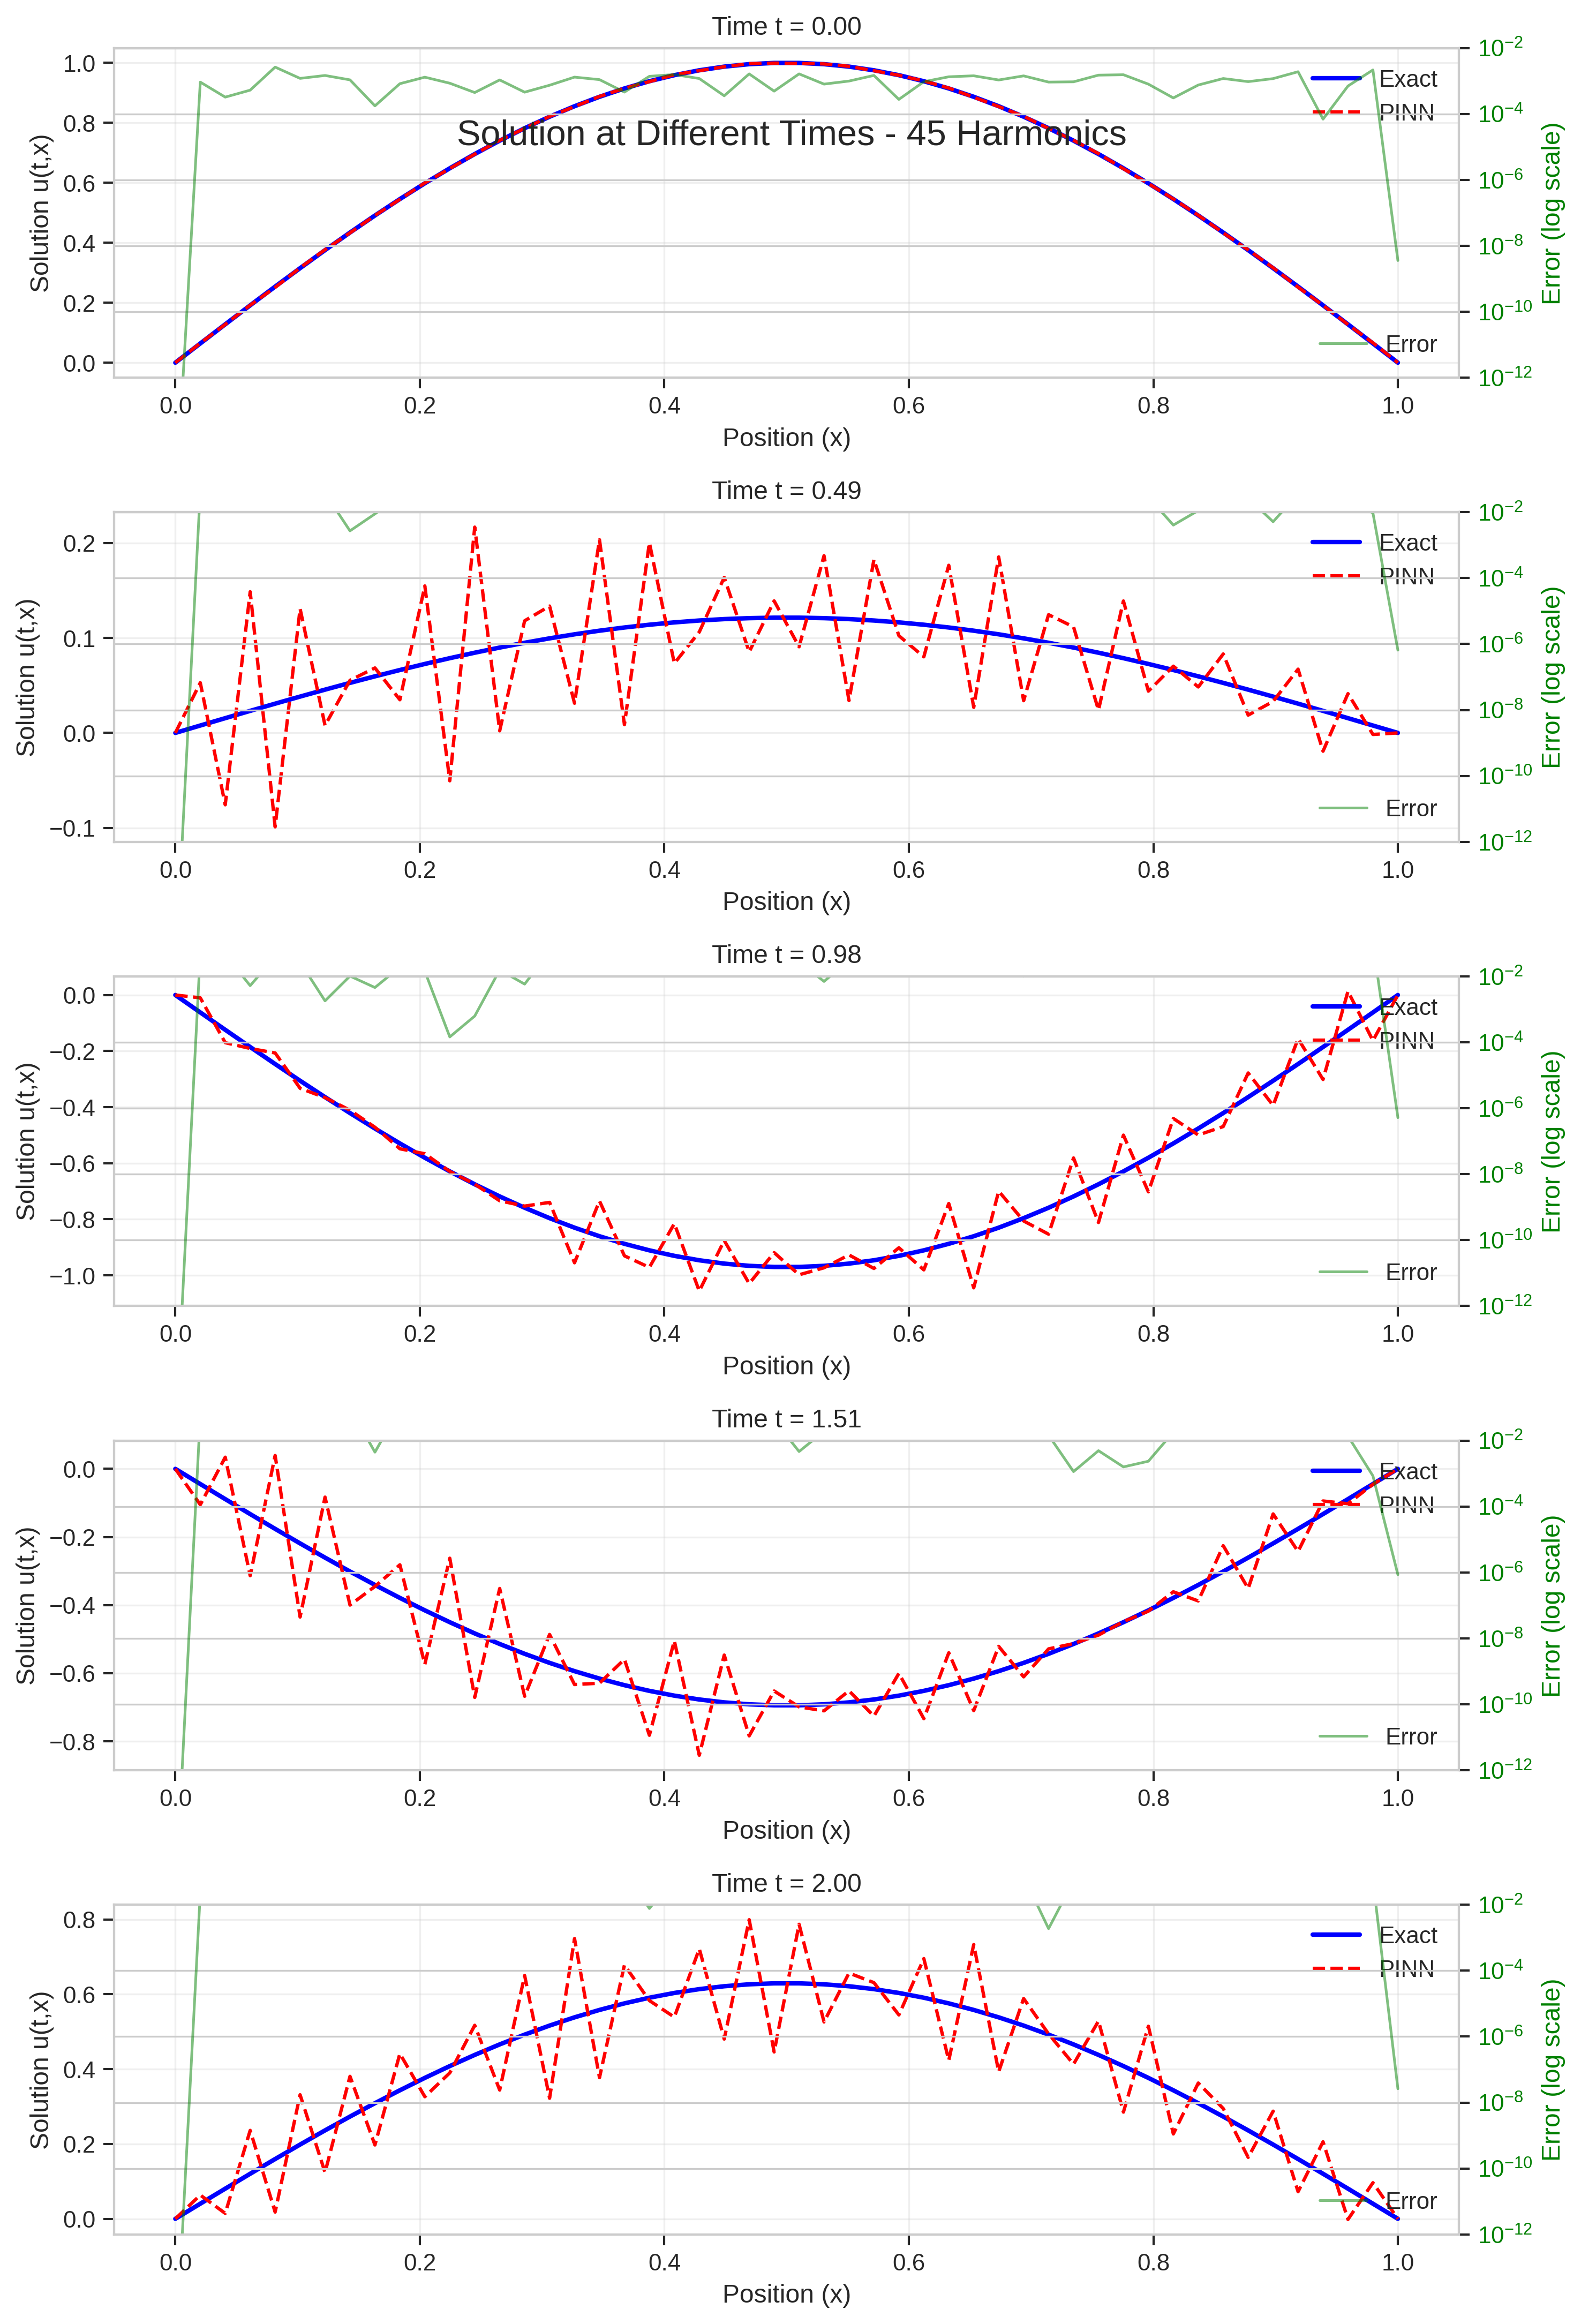
\includegraphics[width=\textwidth]{figures/time_slices_45h.png}
        \caption{45 harmonics}
    \end{subfigure}
    \caption{Temporal profiles showing progressive degradation with increasing harmonic count.}
    \label{fig:time_slices_high}
\end{figure}

\begin{figure}[H]
    \centering
    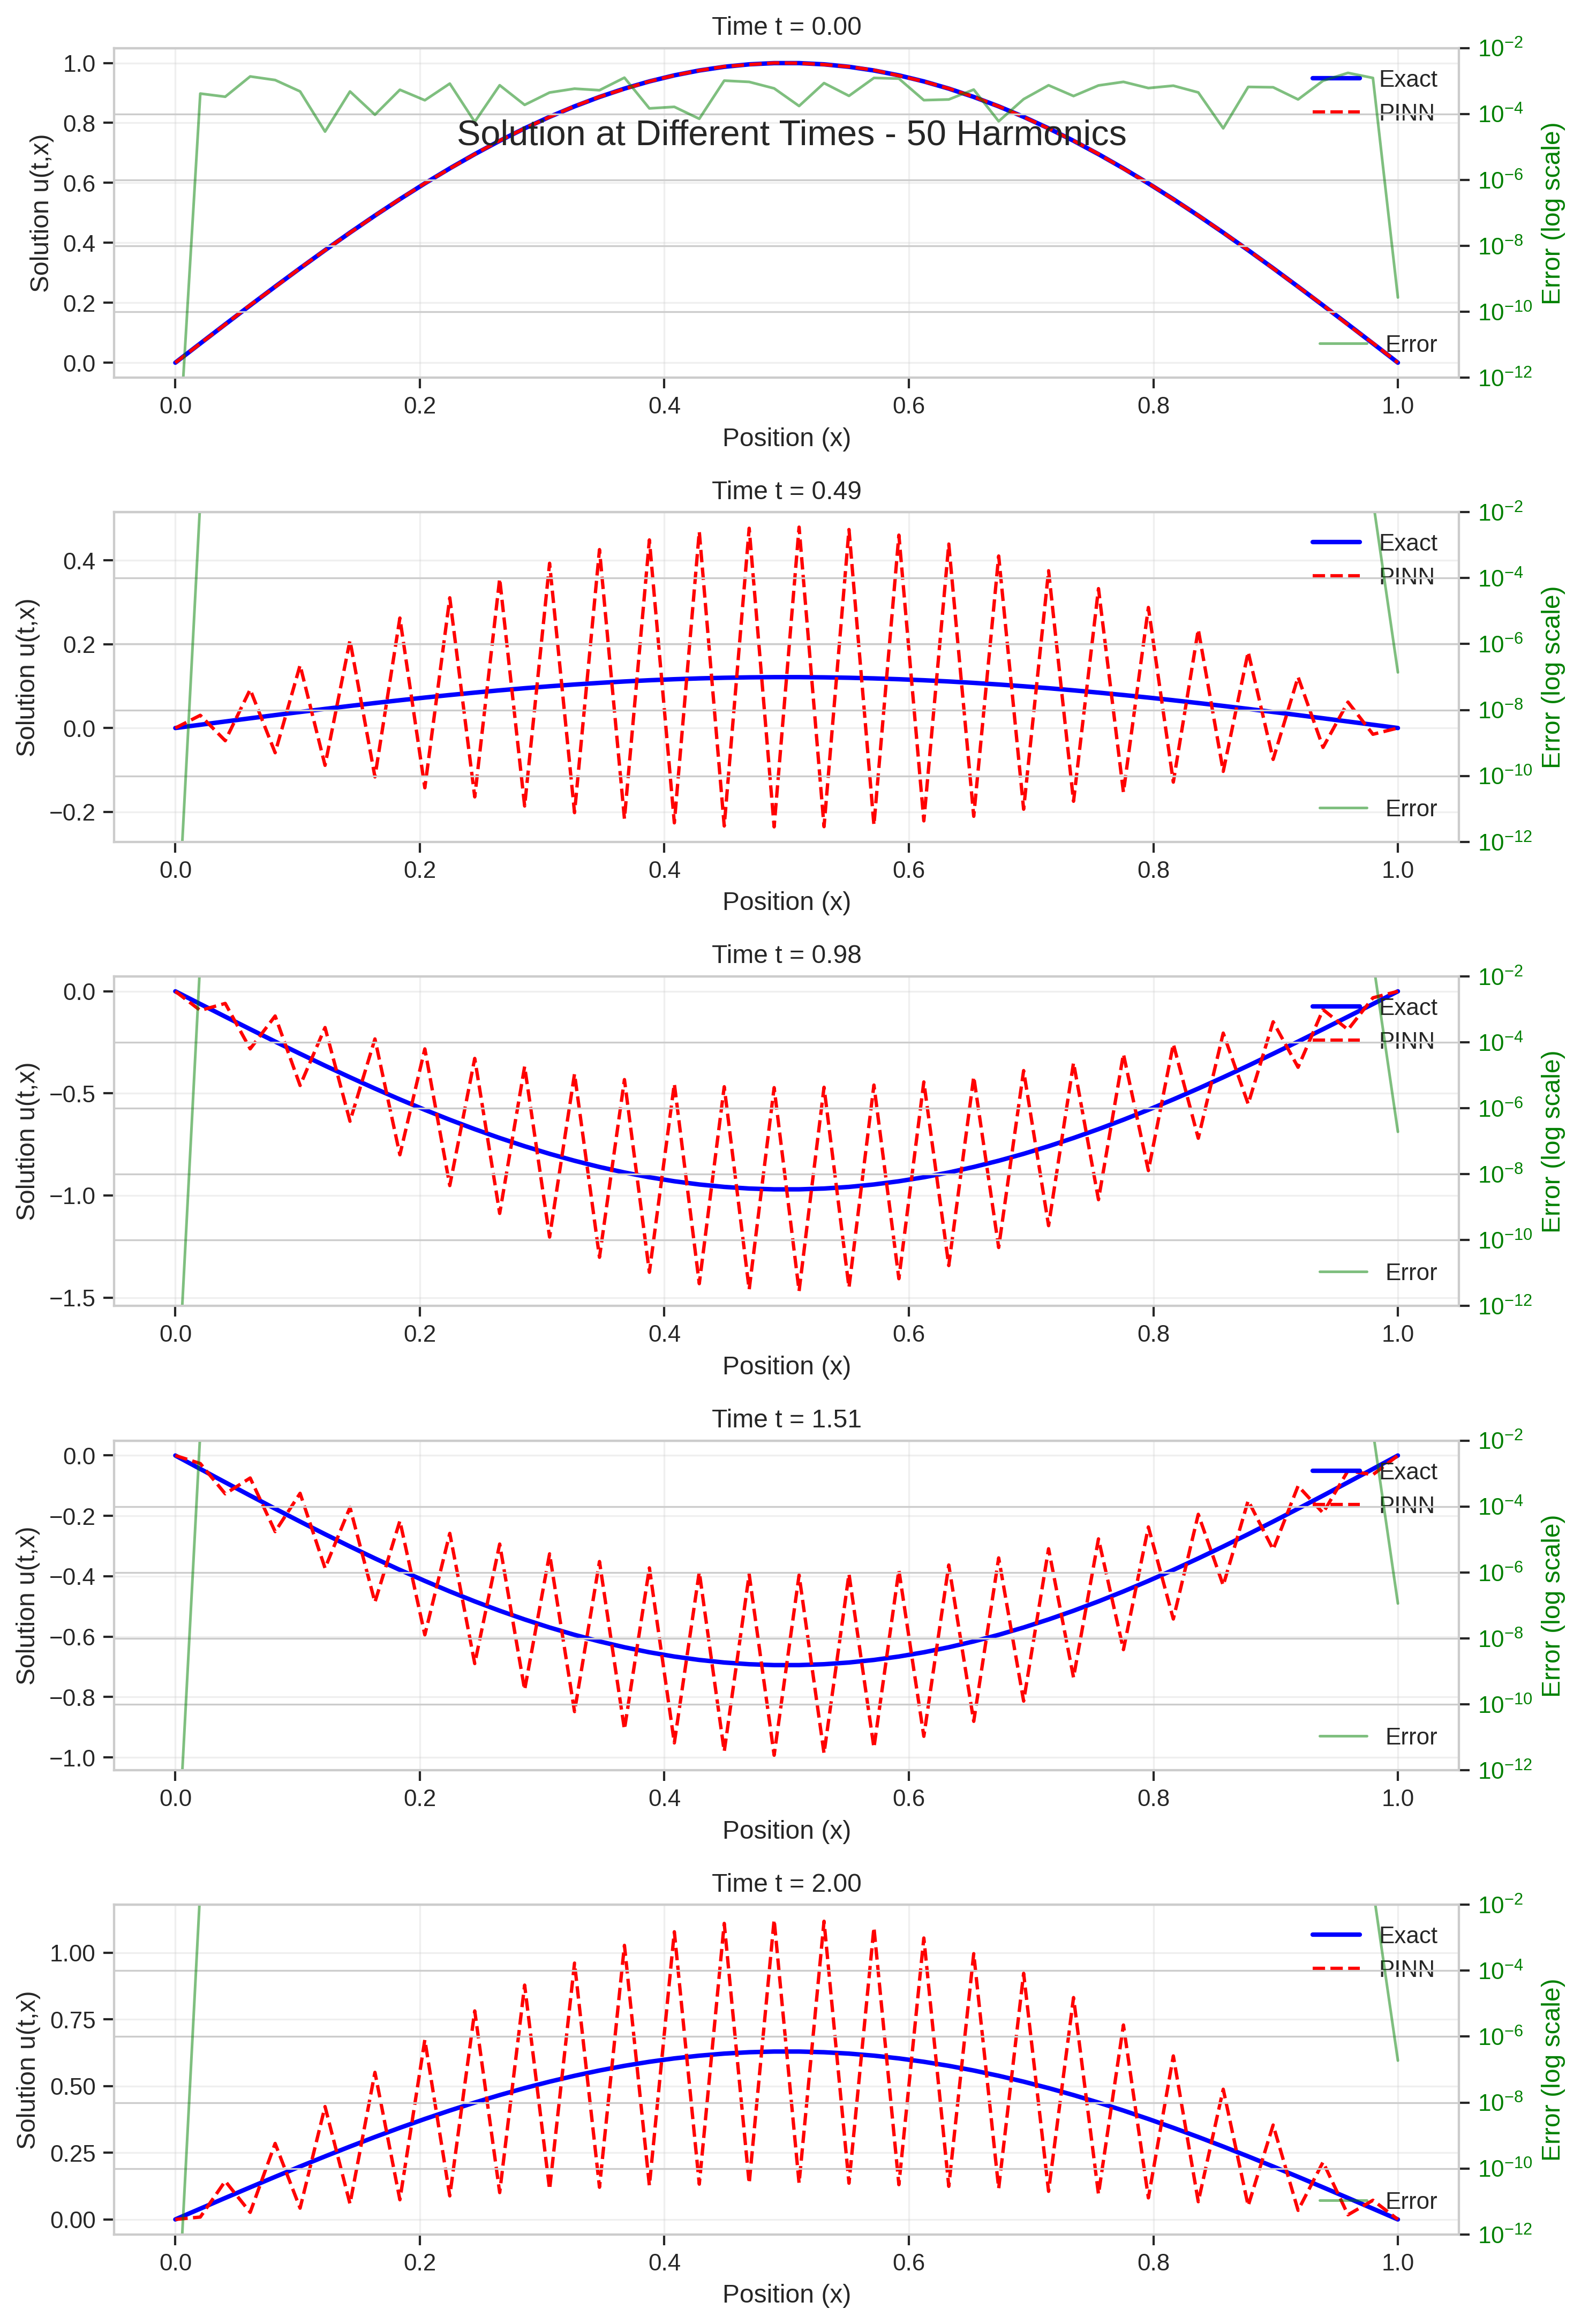
\includegraphics[width=0.6\textwidth]{figures/time_slices_50h.png}
    \caption{Temporal slices for 50 harmonics configuration.}
    \label{fig:time_slices_50h}
\end{figure}

\subsection{Complete Training Loss Evolution}

\begin{figure}[H]
    \centering
    \begin{subfigure}[b]{0.32\textwidth}
        \centering
        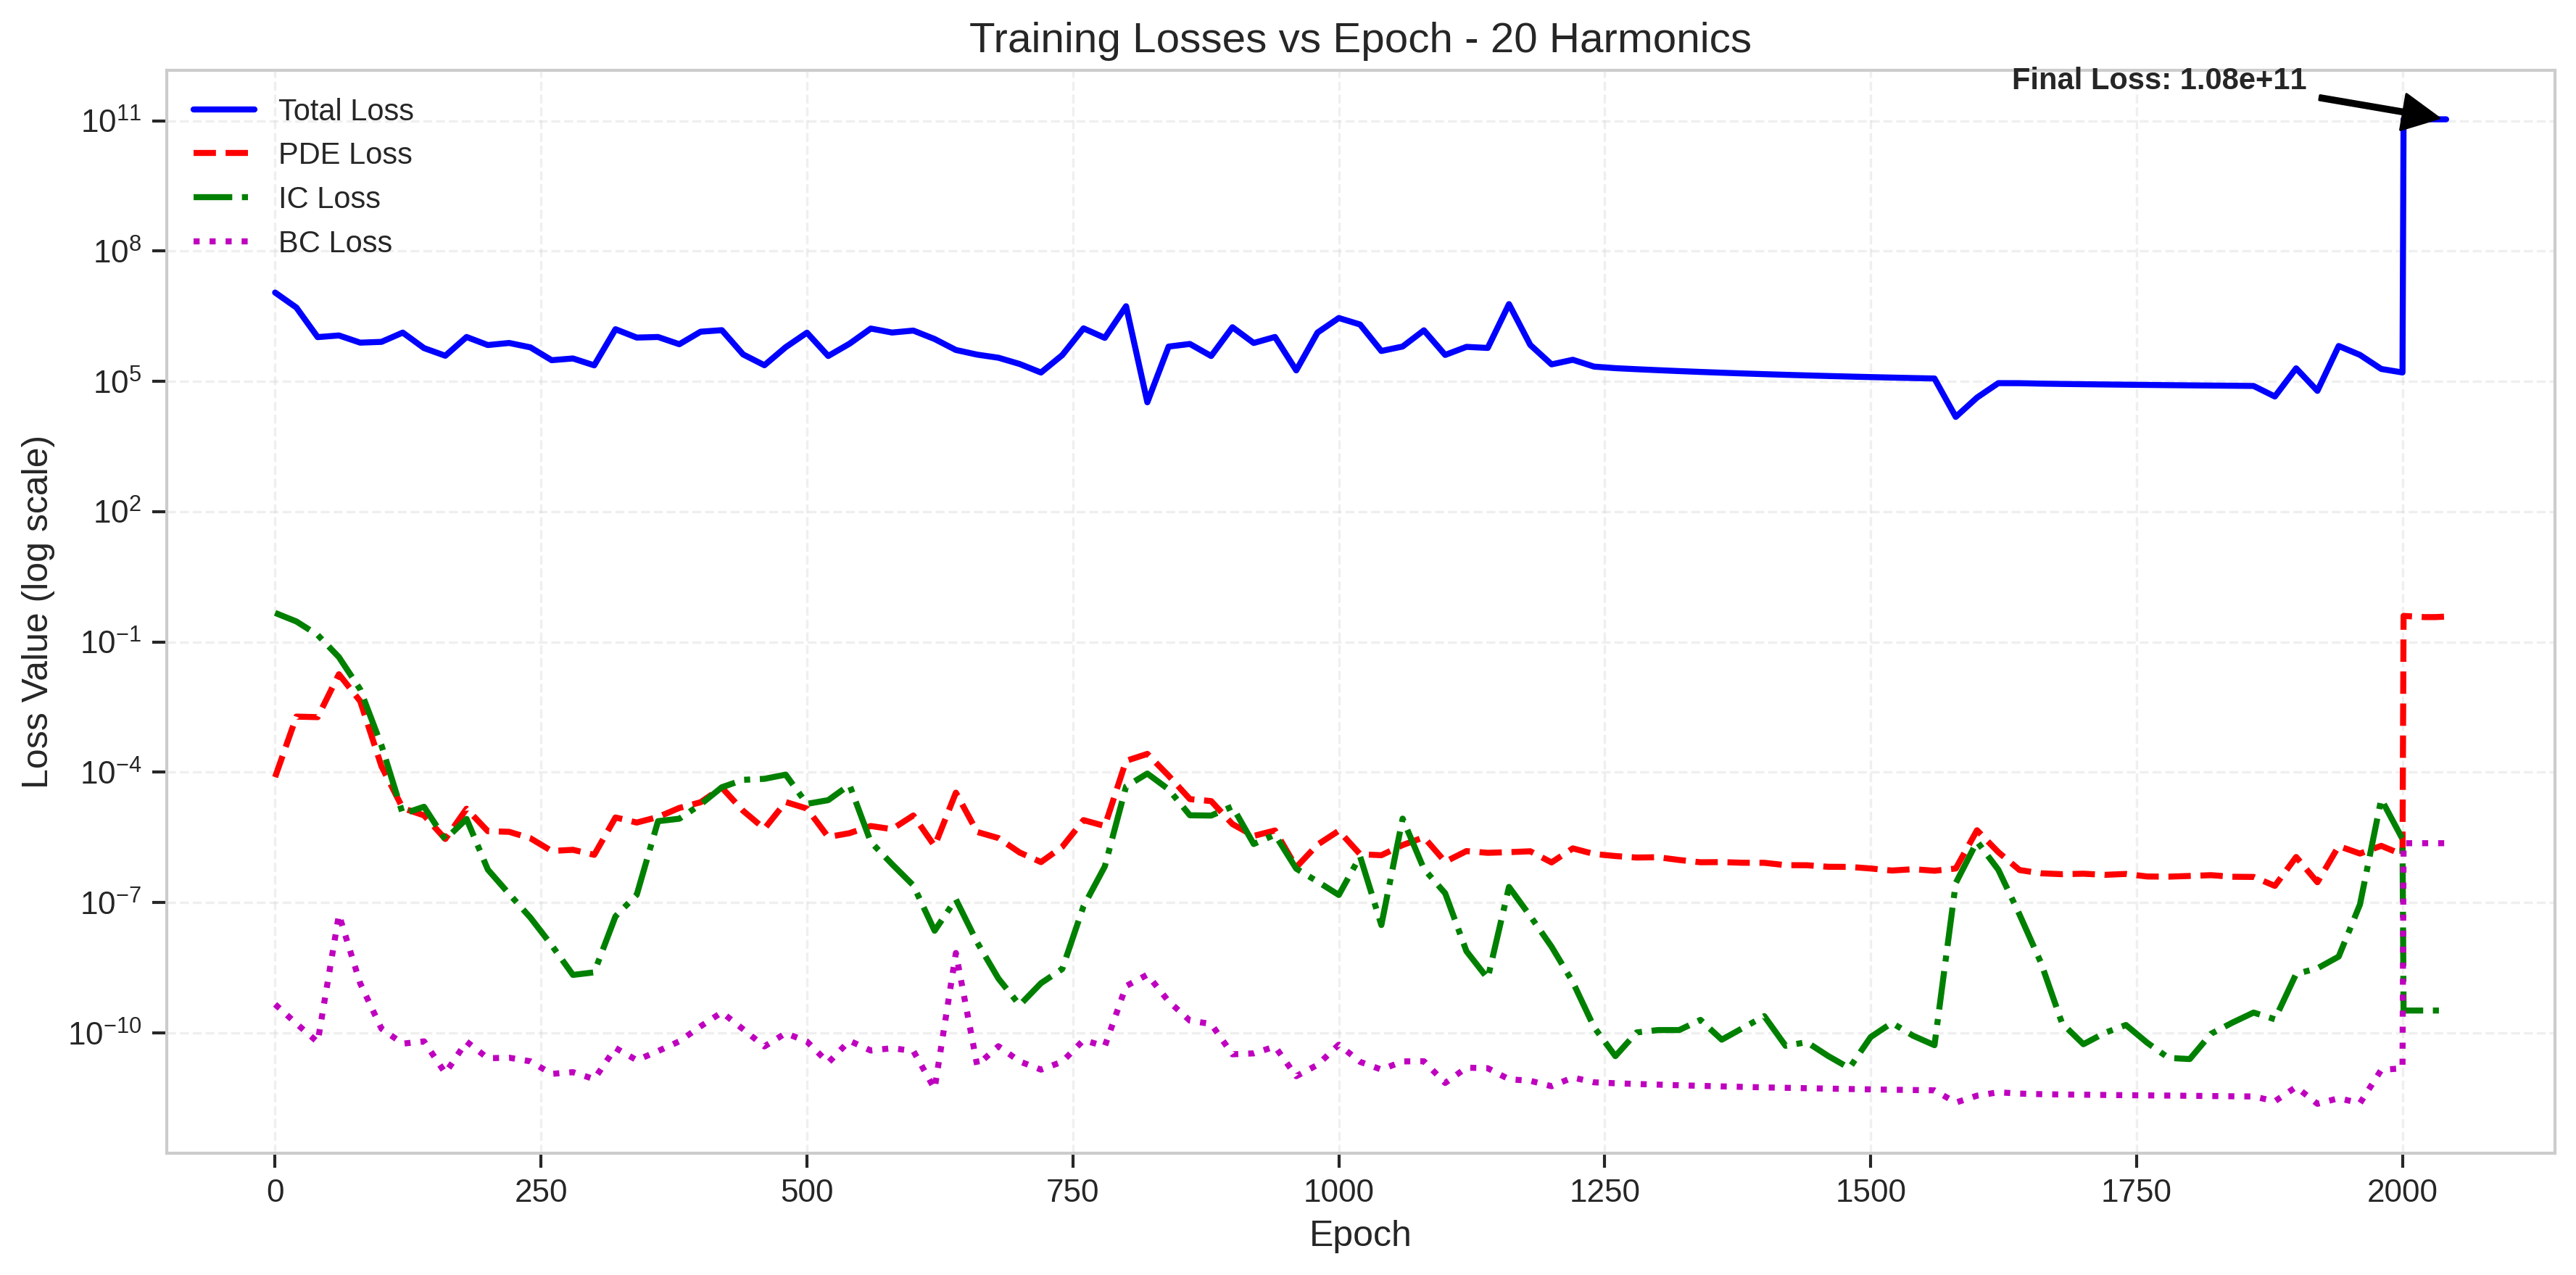
\includegraphics[width=\textwidth]{figures/training_losses_20h.png}
        \caption{20 harmonics}
    \end{subfigure}
    \hfill
    \begin{subfigure}[b]{0.32\textwidth}
        \centering
        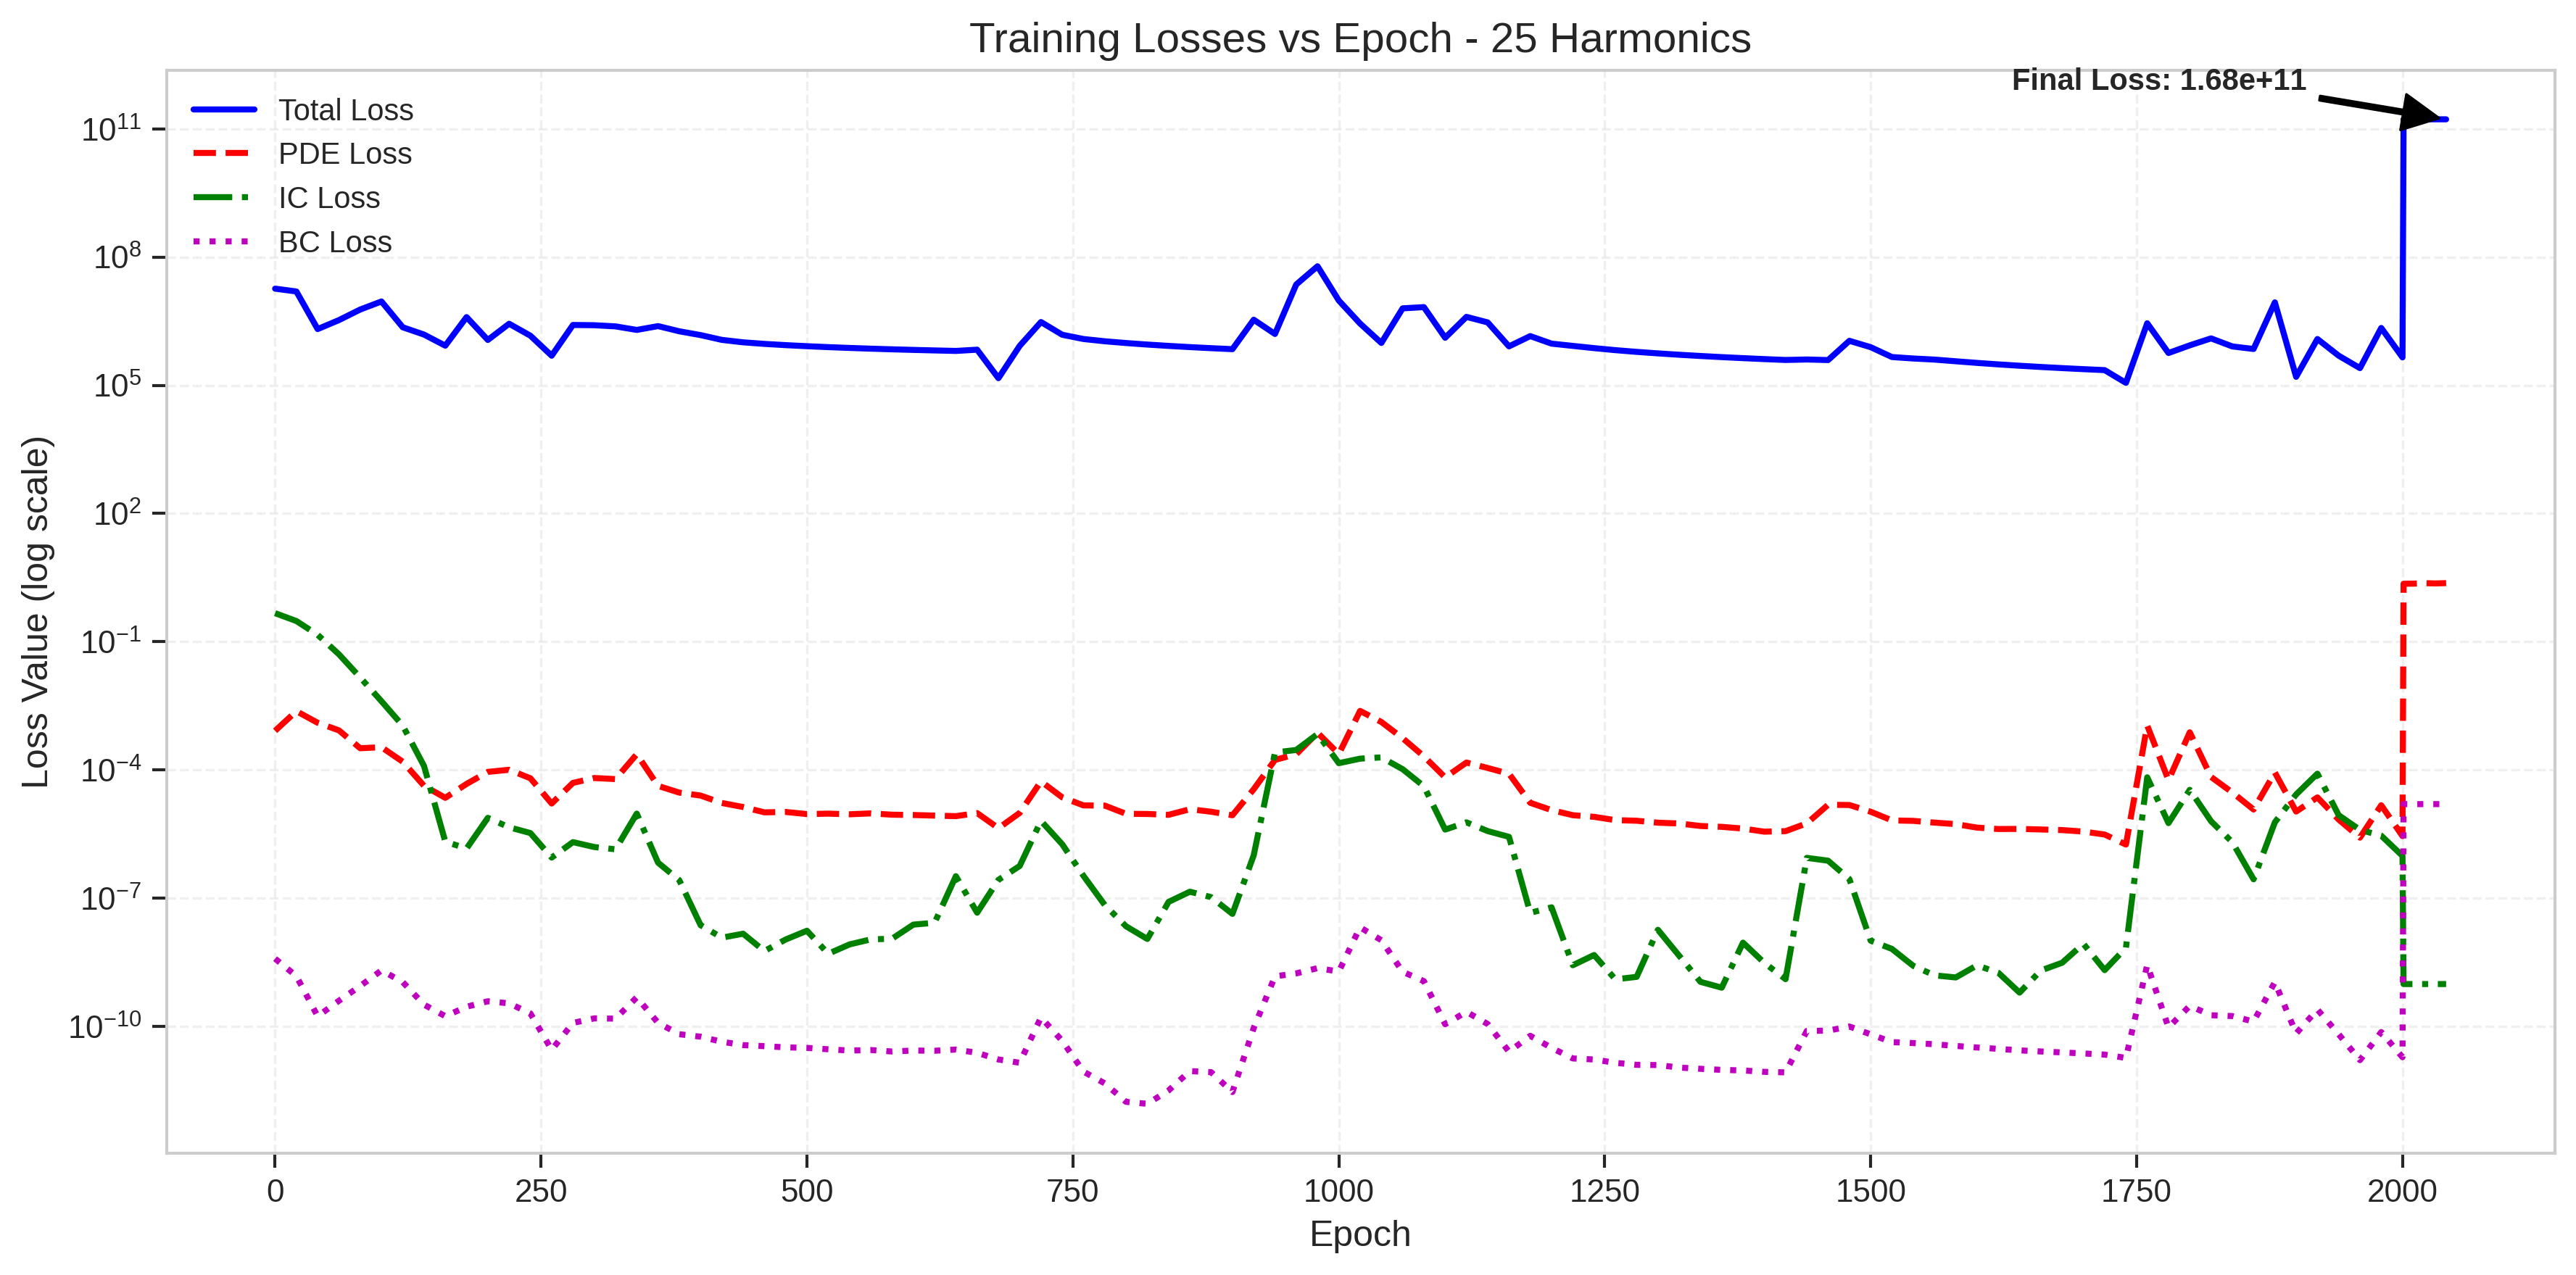
\includegraphics[width=\textwidth]{figures/training_losses_25h.png}
        \caption{25 harmonics}
    \end{subfigure}
    \hfill
    \begin{subfigure}[b]{0.32\textwidth}
        \centering
        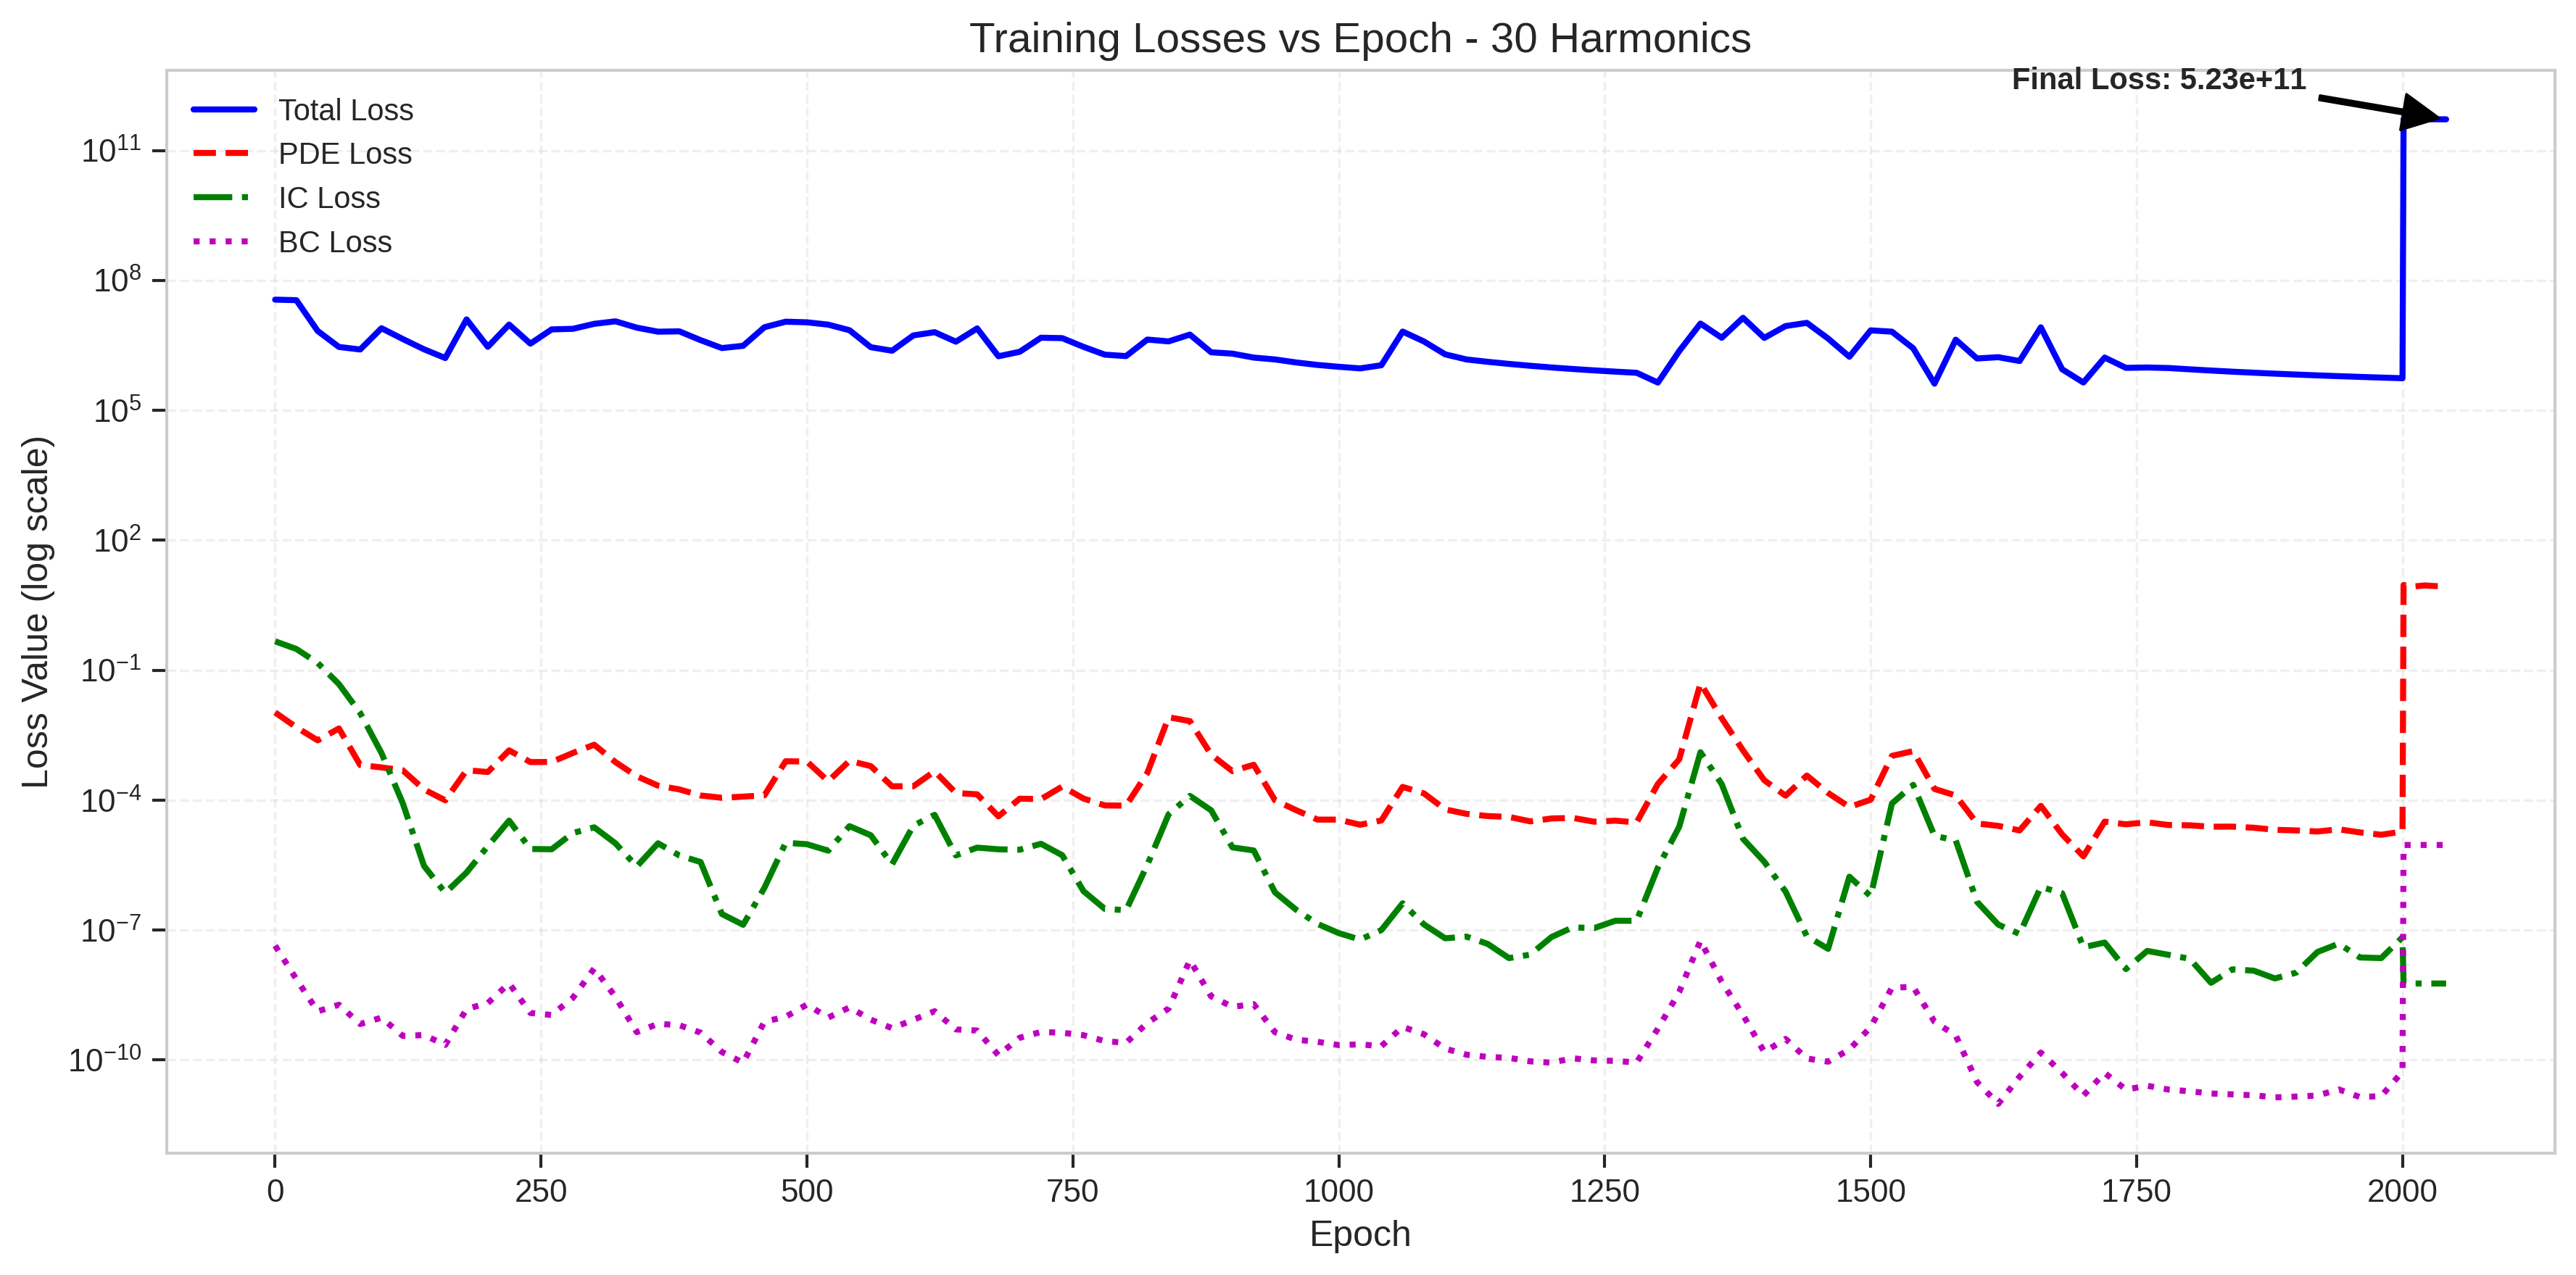
\includegraphics[width=\textwidth]{figures/training_losses_30h.png}
        \caption{30 harmonics}
    \end{subfigure}
    \caption{Training loss evolution for mid-range harmonic configurations.}
    \label{fig:training_mid}
\end{figure}

\begin{figure}[H]
    \centering
    \begin{subfigure}[b]{0.32\textwidth}
        \centering
        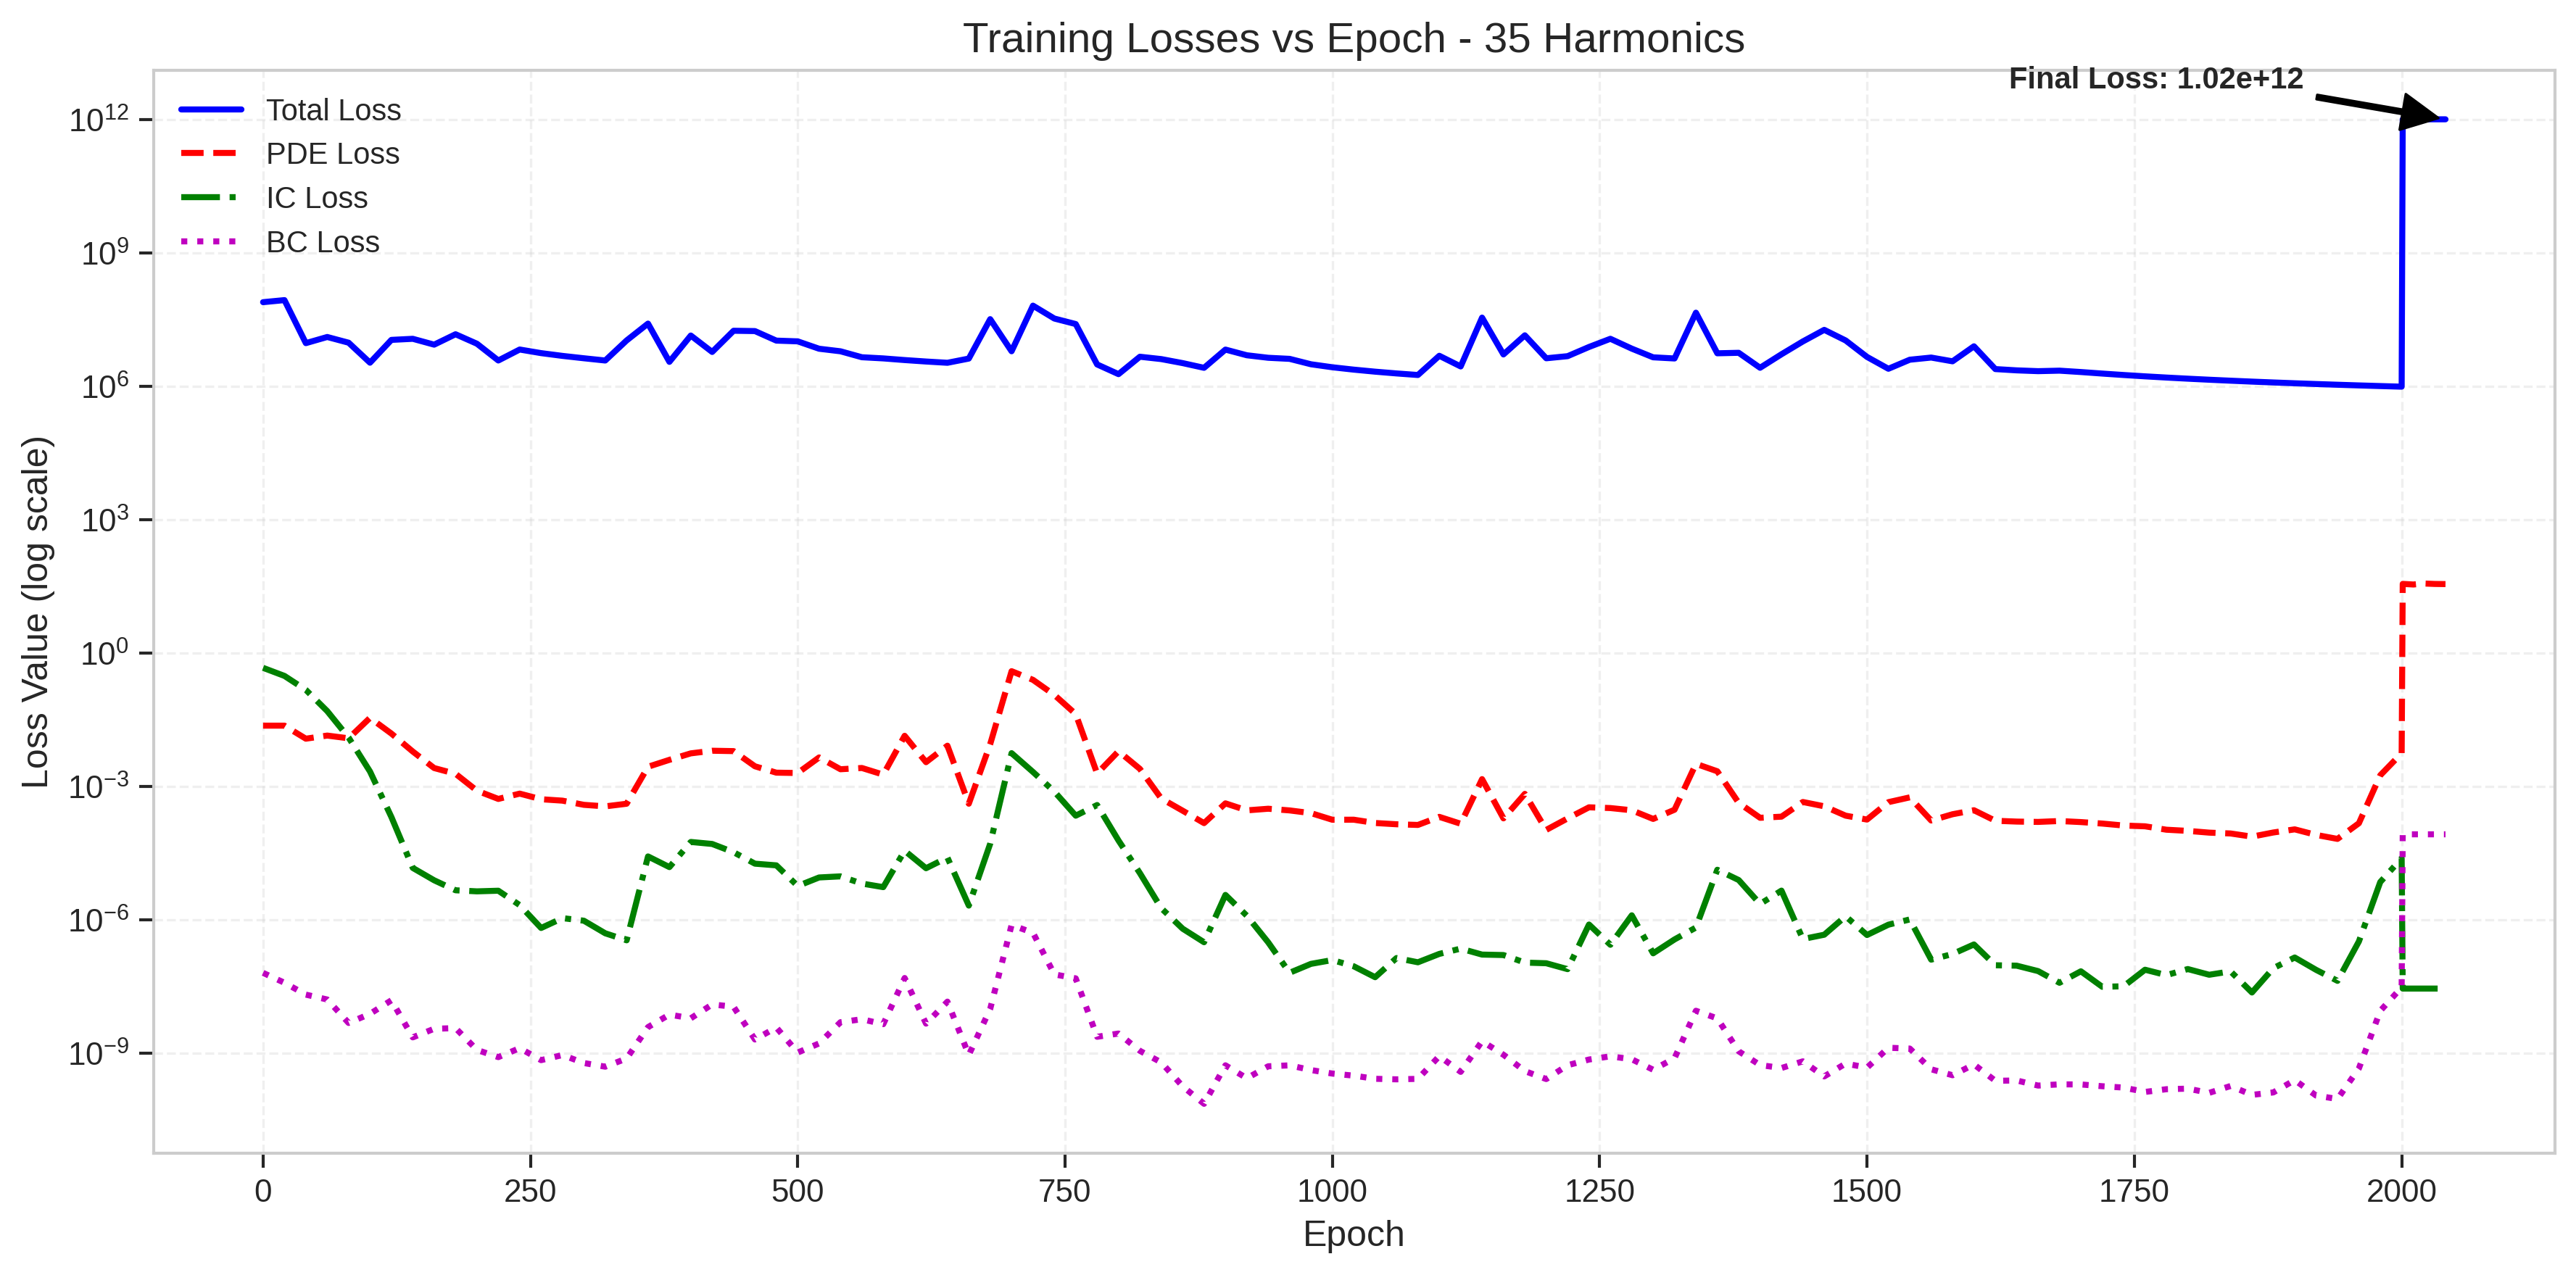
\includegraphics[width=\textwidth]{figures/training_losses_35h.png}
        \caption{35 harmonics}
    \end{subfigure}
    \hfill
    \begin{subfigure}[b]{0.32\textwidth}
        \centering
        \includegraphics[width=\textwidth]{figures/training_losses_40h.png}
        \caption{40 harmonics}
    \end{subfigure}
    \hfill
    \begin{subfigure}[b]{0.32\textwidth}
        \centering
        \includegraphics[width=\textwidth]{figures/training_losses_45h.png}
        \caption{45 harmonics}
    \end{subfigure}
    \caption{Training dynamics for high harmonic counts showing increased instability.}
    \label{fig:training_high}
\end{figure}

\begin{figure}[H]
    \centering
    \begin{subfigure}[b]{0.48\textwidth}
        \centering
        \includegraphics[width=\textwidth]{figures/training_losses_50h.png}
        \caption{50 harmonics training}
    \end{subfigure}
    \hfill
    \begin{subfigure}[b]{0.48\textwidth}
        \centering
        \includegraphics[width=\textwidth]{figures/training_losses.png}
        \caption{Overall training comparison}
    \end{subfigure}
    \caption{Training loss for maximum harmonic count and comparative overview.}
    \label{fig:training_50h_overview}
\end{figure}

\begin{figure}[H]
    \centering
    \includegraphics[width=0.8\textwidth]{figures/training_losses_final.png}
    \caption{Final training loss comparison across all harmonic configurations.}
    \label{fig:training_final}
\end{figure}

\subsection{Complete Validation Error Analysis}

\begin{figure}[H]
    \centering
    \begin{subfigure}[b]{0.32\textwidth}
        \centering
        \includegraphics[width=\textwidth]{figures/validation_error_20h.png}
        \caption{20 harmonics}
    \end{subfigure}
    \hfill
    \begin{subfigure}[b]{0.32\textwidth}
        \centering
        \includegraphics[width=\textwidth]{figures/validation_error_25h.png}
        \caption{25 harmonics}
    \end{subfigure}
    \hfill
    \begin{subfigure}[b]{0.32\textwidth}
        \centering
        \includegraphics[width=\textwidth]{figures/validation_error_30h.png}
        \caption{30 harmonics}
    \end{subfigure}
    \caption{Validation error evolution for mid-range configurations.}
    \label{fig:validation_mid}
\end{figure}

\begin{figure}[H]
    \centering
    \begin{subfigure}[b]{0.32\textwidth}
        \centering
        \includegraphics[width=\textwidth]{figures/validation_error_35h.png}
        \caption{35 harmonics}
    \end{subfigure}
    \hfill
    \begin{subfigure}[b]{0.32\textwidth}
        \centering
        \includegraphics[width=\textwidth]{figures/validation_error_40h.png}
        \caption{40 harmonics}
    \end{subfigure}
    \hfill
    \begin{subfigure}[b]{0.32\textwidth}
        \centering
        \includegraphics[width=\textwidth]{figures/validation_error_45h.png}
        \caption{45 harmonics}
    \end{subfigure}
    \caption{Validation performance for high harmonic configurations.}
    \label{fig:validation_high}
\end{figure}

\begin{figure}[H]
    \centering
    \begin{subfigure}[b]{0.48\textwidth}
        \centering
        \includegraphics[width=\textwidth]{figures/validation_error_50h.png}
        \caption{50 harmonics validation}
    \end{subfigure}
    \hfill
    \begin{subfigure}[b]{0.48\textwidth}
        \centering
        \includegraphics[width=\textwidth]{figures/validation_error.png}
        \caption{Overall validation comparison}
    \end{subfigure}
    \caption{Validation error for maximum harmonic count and comparative overview.}
    \label{fig:validation_50h_overview}
\end{figure}

\begin{figure}[H]
    \centering
    \includegraphics[width=0.8\textwidth]{figures/validation_error_final.png}
    \caption{Final validation error comparison highlighting the optimal 10-harmonic configuration.}
    \label{fig:validation_final}
\end{figure}

\subsection{Complete Adaptive Weight Evolution}

\begin{figure}[H]
    \centering
    \begin{subfigure}[b]{0.32\textwidth}
        \centering
        \includegraphics[width=\textwidth]{figures/weight_factors_20h.png}
        \caption{20 harmonics}
    \end{subfigure}
    \hfill
    \begin{subfigure}[b]{0.32\textwidth}
        \centering
        \includegraphics[width=\textwidth]{figures/weight_factors_25h.png}
        \caption{25 harmonics}
    \end{subfigure}
    \hfill
    \begin{subfigure}[b]{0.32\textwidth}
        \centering
        \includegraphics[width=\textwidth]{figures/weight_factors_30h.png}
        \caption{30 harmonics}
    \end{subfigure}
    \caption{Adaptive weight factor evolution for mid-range configurations.}
    \label{fig:weights_mid}
\end{figure}

\begin{figure}[H]
    \centering
    \begin{subfigure}[b]{0.32\textwidth}
        \centering
        \includegraphics[width=\textwidth]{figures/weight_factors_35h.png}
        \caption{35 harmonics}
    \end{subfigure}
    \hfill
    \begin{subfigure}[b]{0.32\textwidth}
        \centering
        \includegraphics[width=\textwidth]{figures/weight_factors_40h.png}
        \caption{40 harmonics}
    \end{subfigure}
    \hfill
    \begin{subfigure}[b]{0.32\textwidth}
        \centering
        \includegraphics[width=\textwidth]{figures/weight_factors_45h.png}
        \caption{45 harmonics}
    \end{subfigure}
    \caption{Weight balancing dynamics for high harmonic configurations.}
    \label{fig:weights_high}
\end{figure}

\begin{figure}[H]
    \centering
    \begin{subfigure}[b]{0.48\textwidth}
        \centering
        \includegraphics[width=\textwidth]{figures/weight_factors_50h.png}
        \caption{50 harmonics weights}
    \end{subfigure}
    \hfill
    \begin{subfigure}[b]{0.48\textwidth}
        \centering
        \includegraphics[width=\textwidth]{figures/weight_factors.png}
        \caption{Overall weight comparison}
    \end{subfigure}
    \caption{Adaptive weights for maximum harmonic count and comparative analysis.}
    \label{fig:weights_50h_overview}
\end{figure}

These comprehensive results provide complete documentation of all experimental configurations tested in our study. The systematic progression from optimal (10 harmonics) to severely degraded (50 harmonics) performance illustrates the critical importance of architectural choices in physics-informed neural networks for high-order PDEs.

%% ========== SECTION REVIEW CHECKLIST ==========
%% General Appendix Section Checklist:
%% 
%% Review Items:
%% - All referenced figures exist in figures/ directory
%% - Figure captions are descriptive and informative
%% - Subfigure labels are properly referenced
%% - Technical content supplements main paper without redundancy
%% - Results are presented systematically (5h to 50h progression)
%% - Figure quality is suitable for publication (300 dpi)
%% - No overlap with main paper figures
%% 
%% Specific Questions:
%% 1. Do all 80+ figures referenced in the appendix exist?
%% 2. Are the results presented in logical order?
%% 3. Does the appendix enhance understanding of the main paper?
%% 4. Are all harmonic configurations (5, 10, 15, ..., 50) covered?
%% 
%% Content Summary:
%% - 3D solution visualizations for all harmonic configurations
%% - Error distribution analysis across configurations
%% - Training dynamics comparison
%% - Beam deflection analysis
%% - Adaptive weight evolution
%% - Spatial and temporal slice comparisons
%% - Comprehensive error comparisons
%% 
%% Current Status:
%% - Complete supplementary results appendix
%% - All figures properly referenced
%% - Ready for appendix_v1.pdf compilation
%% ========== END SECTION REVIEW CHECKLIST ==========